\documentclass[twoside]{article}

% Packages required by doxygen
\usepackage{fixltx2e}
\usepackage{calc}
\usepackage{doxygen}
\usepackage[export]{adjustbox} % also loads graphicx
\usepackage{graphicx}
\usepackage[utf8]{inputenc}
\usepackage{makeidx}
\usepackage{multicol}
\usepackage{multirow}
\PassOptionsToPackage{warn}{textcomp}
\usepackage{textcomp}
\usepackage[nointegrals]{wasysym}
\usepackage[table]{xcolor}

% NLS support packages
\usepackage[french]{babel}

% Font selection
\usepackage[T1]{fontenc}
\usepackage[scaled=.90]{helvet}
\usepackage{courier}
\usepackage{amssymb}
\usepackage{sectsty}
\renewcommand{\familydefault}{\sfdefault}
\allsectionsfont{%
  \fontseries{bc}\selectfont%
  \color{darkgray}%
}
\renewcommand{\DoxyLabelFont}{%
  \fontseries{bc}\selectfont%
  \color{darkgray}%
}
\newcommand{\+}{\discretionary{\mbox{\scriptsize$\hookleftarrow$}}{}{}}

% Page & text layout
\usepackage[a4paper]{geometry}
\geometry{vmargin=2cm,hmargin=2cm,lmargin=1.2cm,rmargin=1.2cm}
% \usepackage{geometry}
% \geometry{%
%   a4paper,%
%   top=2.5cm,%
%   bottom=2.5cm,%
%   left=2.5cm,%
%   right=2.5cm%
% }
\tolerance=750
\hfuzz=15pt
\hbadness=750
\setlength{\emergencystretch}{15pt}
\setlength{\parindent}{0cm}
\setlength{\parskip}{3ex plus 2ex minus 2ex}
\makeatletter
\renewcommand{\paragraph}{%
  \@startsection{paragraph}{4}{0ex}{-1.0ex}{1.0ex}{%
    \normalfont\normalsize\bfseries\SS@parafont%
  }%
}
\renewcommand{\subparagraph}{%
  \@startsection{subparagraph}{5}{0ex}{-1.0ex}{1.0ex}{%
    \normalfont\normalsize\bfseries\SS@subparafont%
  }%
}
\makeatother

% Headers & footers
\usepackage{fancyhdr}
\pagestyle{fancyplain}
\fancyhead[LE]{\fancyplain{}{\bfseries\thepage}}
\fancyhead[CE]{\fancyplain{}{}}
\fancyhead[RE]{\fancyplain{}{\bfseries\leftmark}}
\fancyhead[LO]{\fancyplain{}{\bfseries\rightmark}}
\fancyhead[CO]{\fancyplain{}{}}
\fancyhead[RO]{\fancyplain{}{\bfseries\thepage}}
\fancyfoot[LE]{\fancyplain{}{\bfseries\scriptsize Rov'Net}}
\fancyfoot[CE]{\fancyplain{}{}}
\fancyfoot[RE]{\fancyplain{}{\bfseries\scriptsize BTS SN-IR LaSalle Avigon 2019 }}
\fancyfoot[LO]{\fancyplain{}{\bfseries\scriptsize BTS SN-IR LaSalle Avigon 2019 }}
\fancyfoot[CO]{\fancyplain{}{}}
\fancyfoot[RO]{\fancyplain{}{\bfseries\scriptsize Rov'Net}}
\renewcommand{\footrulewidth}{0.4pt}
\renewcommand{\sectionmark}[1]{%
  \markright{\thesection\ #1}%
}

% Indices & bibliography
\usepackage{natbib}
\usepackage[titles]{tocloft}
\setcounter{tocdepth}{3}
\setcounter{secnumdepth}{5}
\makeindex

% Hyperlinks (required, but should be loaded last)
\usepackage{ifpdf}
\ifpdf
  \usepackage[pdftex,pagebackref=true]{hyperref}
\else
  \usepackage[ps2pdf,pagebackref=true]{hyperref}
\fi
\hypersetup{%
  colorlinks=true,%
  linkcolor=blue,%
  citecolor=blue,%
  unicode%
}

% Custom commands
\newcommand{\clearemptydoublepage}{%
  \newpage{\pagestyle{empty}\cleardoublepage}%
}

\usepackage{caption}
\captionsetup{labelsep=space,justification=centering,font={bf},singlelinecheck=off,skip=4pt,position=top}

%===== C O N T E N T S =====

\begin{document}

% Titlepage & ToC
\hypersetup{pageanchor=false,
             bookmarksnumbered=true,
             pdfencoding=unicode
            }
\pagenumbering{alph}
\begin{titlepage}
\vspace*{7cm}
\begin{center}%
{\LARGE Projet R\+OV\textquotesingle{}N\+ET \\[1ex]\large 1.\+1 }\\
\vspace*{1cm}
{\large BTS SN-IR LaSalle Avignon 2019}\\
\vspace*{1cm}
{\large REYNIER Jacques}\\
{\large BOFFREDO Nicolas}\\
\end{center}
\end{titlepage}
\pagenumbering{roman}
\tableofcontents
\pagenumbering{arabic}
\hypersetup{pageanchor=true}

%--- Begin generated contents ---
\section{Le projet R\+OV\textquotesingle{}N\+ET}
\label{index}\hypertarget{index}{}Le système R\+OV\textquotesingle{}N\+ET est capable d\textquotesingle{}obtenir et gérer des données d\textquotesingle{}entrée afin de définir un environnement T\+QC (Tel Que Construit) en se déplaçant dans un milieu contaminé.

\begin{DoxyAuthor}{Auteur}
{\itshape B\+O\+F\+F\+R\+E\+DO} Nicolas \href{mailto:nboffredo@gmail.com}{\tt nboffredo@gmail.\+com}

{\itshape R\+E\+Y\+N\+I\+ER} Jacques \href{mailto:reynier.jacques@gmail.com}{\tt reynier.\+jacques@gmail.\+com}
\end{DoxyAuthor}
\hypertarget{index_section_tdm}{}\subsection{Table des matières}\label{index_section_tdm}

\begin{DoxyItemize}
\item \hyperlink{page__r_e_a_d_m_e}{R\+E\+A\+D\+ME}
\item \hyperlink{page_changelog}{Changelog}
\item \hyperlink{page_install}{Installation}
\item \hyperlink{page_about}{A propos}
\item \hyperlink{page_licence}{Licence G\+PL} 
\end{DoxyItemize}
\section{Changelog}
\label{page_changelog}
\Hypertarget{page_changelog}
r137 $\vert$ jreynier $\vert$ 2019-\/06-\/05 16\+:16\+:38 +0200 (mer. 05 juin 2019) $\vert$ 1 ligne

Modification des déplacements (provisoire).

r136 $\vert$ nboffredo $\vert$ 2019-\/06-\/04 17\+:17\+:17 +0200 (mar. 04 juin 2019) $\vert$ 1 ligne

Correction trame déplacement caméra

r135 $\vert$ nboffredo $\vert$ 2019-\/06-\/04 17\+:06\+:42 +0200 (mar. 04 juin 2019) $\vert$ 1 ligne

Modificatoin trame déplacement caméra

r134 $\vert$ nboffredo $\vert$ 2019-\/06-\/04 16\+:56\+:03 +0200 (mar. 04 juin 2019) $\vert$ 1 ligne

Correction liste des caméras

r133 $\vert$ jreynier $\vert$ 2019-\/06-\/04 16\+:26\+:53 +0200 (mar. 04 juin 2019) $\vert$ 1 ligne

Ajout de la fenêtre de Paramètres à la création d\textquotesingle{}une nouvelle campagne.

r132 $\vert$ nboffredo $\vert$ 2019-\/06-\/04 15\+:07\+:56 +0200 (mar. 04 juin 2019) $\vert$ 1 ligne

Correction d\textquotesingle{}un crash + départ du chronomètre mis au départ d\textquotesingle{}une nouvelle campagne

r131 $\vert$ nboffredo $\vert$ 2019-\/06-\/04 13\+:57\+:00 +0200 (mar. 04 juin 2019) $\vert$ 1 ligne

Correction crash au démarrage d\textquotesingle{}une nouvelle campagne

r130 $\vert$ nboffredo $\vert$ 2019-\/06-\/04 12\+:14\+:42 +0200 (mar. 04 juin 2019) $\vert$ 1 ligne

Correction bug remplissage liste caméra I\+HM

r129 $\vert$ jreynier $\vert$ 2019-\/06-\/04 12\+:03\+:19 +0200 (mar. 04 juin 2019) $\vert$ 1 ligne

Modification de la fenêtre Paramètres.

r128 $\vert$ jreynier $\vert$ 2019-\/06-\/04 09\+:09\+:33 +0200 (mar. 04 juin 2019) $\vert$ 1 ligne

Ajout d\textquotesingle{}une fenetre d\textquotesingle{}erreur lorsque l\textquotesingle{}on choisi un port indisponible dans la fenetre de parametres + affichage du parametrage dés la création de la campagne.

r127 $\vert$ nboffredo $\vert$ 2019-\/06-\/04 08\+:22\+:59 +0200 (mar. 04 juin 2019) $\vert$ 1 ligne

Correction bug démarrage caméra

r126 $\vert$ nboffredo $\vert$ 2019-\/06-\/04 08\+:18\+:16 +0200 (mar. 04 juin 2019) $\vert$ 1 ligne

mise à jour de la base de donnée (correction des id)

r125 $\vert$ nboffredo $\vert$ 2019-\/06-\/04 08\+:12\+:06 +0200 (mar. 04 juin 2019) $\vert$ 1 ligne

suppression d\textquotesingle{}un operateur

r124 $\vert$ jreynier $\vert$ 2019-\/05-\/29 17\+:41\+:42 +0200 (mer. 29 mai 2019) $\vert$ 1 ligne

Modification envoi de trames

r123 $\vert$ nboffredo $\vert$ 2019-\/05-\/29 11\+:52\+:08 +0200 (mer. 29 mai 2019) $\vert$ 1 ligne

Suppression d\textquotesingle{}un operteur dans la table operateur de la B\+DD

r122 $\vert$ jreynier $\vert$ 2019-\/05-\/29 11\+:46\+:17 +0200 (mer. 29 mai 2019) $\vert$ 1 ligne

Modification de noms de signaux.

r121 $\vert$ jreynier $\vert$ 2019-\/05-\/28 17\+:20\+:20 +0200 (mar. 28 mai 2019) $\vert$ 1 ligne

Ajout de l\textquotesingle{}actualisation des icones d\textquotesingle{}état dans l\textquotesingle{}I\+HM.

r120 $\vert$ jreynier $\vert$ 2019-\/05-\/28 13\+:54\+:21 +0200 (mar. 28 mai 2019) $\vert$ 1 ligne

Mise en fonction de la modification de l\textquotesingle{}intervalle d\textquotesingle{}archivage dans la fenetre de parametres.

r119 $\vert$ jreynier $\vert$ 2019-\/05-\/28 12\+:25\+:35 +0200 (mar. 28 mai 2019) $\vert$ 1 ligne

Mise en fonction du bouton Archiver mesures dans la fenetre de parametres.

r118 $\vert$ tvaira $\vert$ 2019-\/05-\/27 18\+:30\+:13 +0200 (lun. 27 mai 2019) $\vert$ 2 lignes

Vérification Création nouvelle campagne

r117 $\vert$ nboffredo $\vert$ 2019-\/05-\/27 12\+:37\+:21 +0200 (lun. 27 mai 2019) $\vert$ 1 ligne

Ajout de la récupération de l\textquotesingle{}id\+Operateur correspondant à l\textquotesingle{}opérateur sélèctionné dans la fenetre de création d\textquotesingle{}une nouvelle campagne

r116 $\vert$ nboffredo $\vert$ 2019-\/05-\/24 12\+:29\+:43 +0200 (ven. 24 mai 2019) $\vert$ 1 ligne

Mise à jour de la création d\textquotesingle{}une nouvelle campagne

r115 $\vert$ jreynier $\vert$ 2019-\/05-\/24 08\+:09\+:50 +0200 (ven. 24 mai 2019) $\vert$ 1 ligne

Ajout d\textquotesingle{}un accesseur pour id\+Campagne de la classe \hyperlink{class_base_de_donnees}{Base\+De\+Donnees}

r114 $\vert$ jreynier $\vert$ 2019-\/05-\/23 16\+:43\+:34 +0200 (jeu. 23 mai 2019) $\vert$ 1 ligne

Mise à jour de l\textquotesingle{}archivage des mesures

r113 $\vert$ nboffredo $\vert$ 2019-\/05-\/23 15\+:54\+:07 +0200 (jeu. 23 mai 2019) $\vert$ 1 ligne

Ajout de la possibilité de démarrer une nouvelle campagne et mise à jour de la doc doxygen

r112 $\vert$ nboffredo $\vert$ 2019-\/05-\/23 10\+:53\+:43 +0200 (jeu. 23 mai 2019) $\vert$ 1 ligne

Mise à jour de la B\+DD

r111 $\vert$ jreynier $\vert$ 2019-\/05-\/23 10\+:07\+:17 +0200 (jeu. 23 mai 2019) $\vert$ 1 ligne

Ajout de l\textquotesingle{}archivage des mesures toutes les secondes (provisoire).

r110 $\vert$ nboffredo $\vert$ 2019-\/05-\/23 09\+:57\+:37 +0200 (jeu. 23 mai 2019) $\vert$ 1 ligne

Mise à jour de la fenetre pour demarrer une nouvelle campagne

r109 $\vert$ jreynier $\vert$ 2019-\/05-\/23 08\+:30\+:03 +0200 (jeu. 23 mai 2019) $\vert$ 1 ligne

Modification de noms de signaux de la classe \hyperlink{class_mesures}{Mesures}

r108 $\vert$ jreynier $\vert$ 2019-\/05-\/21 10\+:16\+:27 +0200 (mar. 21 mai 2019) $\vert$ 1 ligne

Modification de la méthode traite\+Trame de la classe \hyperlink{class_mesures}{Mesures}

r107 $\vert$ nboffredo $\vert$ 2019-\/05-\/21 08\+:52\+:16 +0200 (mar. 21 mai 2019) $\vert$ 1 ligne

Mise à jour de la fenetre des archives \+: taille fixée

r106 $\vert$ nboffredo $\vert$ 2019-\/05-\/21 08\+:45\+:16 +0200 (mar. 21 mai 2019) $\vert$ 1 ligne

Modification de l\textquotesingle{}accesseur get\+Date\+Image(const Q\+Model\+Index) de la classe Archive (changement d\textquotesingle{}un switch à un Q\+String\+List)

r105 $\vert$ tvaira $\vert$ 2019-\/05-\/20 11\+:24\+:11 +0200 (lun. 20 mai 2019) $\vert$ 1 ligne

Ajout documentation Doxygen pour tag 0.\+2

r104 $\vert$ tvaira $\vert$ 2019-\/05-\/20 11\+:21\+:16 +0200 (lun. 20 mai 2019) $\vert$ 1 ligne

Passage des fichiers Doxygen au format Markdown

r103 $\vert$ tvaira $\vert$ 2019-\/05-\/10 17\+:28\+:58 +0200 (ven. 10 mai 2019) $\vert$ 1 ligne

création du tag 0.\+3

r102 $\vert$ nboffredo $\vert$ 2019-\/05-\/03 12\+:46\+:12 +0200 (ven. 03 mai 2019) $\vert$ 1 ligne

Mise à jour de l\textquotesingle{}affichage des mesures en temps réel sur l\textquotesingle{}ihm

r101 $\vert$ jreynier $\vert$ 2019-\/05-\/03 11\+:58\+:05 +0200 (ven. 03 mai 2019) $\vert$ 1 ligne

Modification classe \hyperlink{class_bras}{Bras} \+: modification de l\textquotesingle{}envoi des trames.

r100 $\vert$ nboffredo $\vert$ 2019-\/05-\/03 10\+:40\+:27 +0200 (ven. 03 mai 2019) $\vert$ 1 ligne

Ajout de l\textquotesingle{}affichage des mesures des capteurs sur l\textquotesingle{}ihm

r99 $\vert$ nboffredo $\vert$ 2019-\/05-\/03 10\+:32\+:16 +0200 (ven. 03 mai 2019) $\vert$ 1 ligne

Ajout de la partie distance dans l\textquotesingle{}affichage des mesures sur l\textquotesingle{}ihm

r98 $\vert$ nboffredo $\vert$ 2019-\/05-\/03 10\+:14\+:23 +0200 (ven. 03 mai 2019) $\vert$ 1 ligne

Ajout de la barre de menu et d\textquotesingle{}une fentre d\textquotesingle{}aide

r97 $\vert$ jreynier $\vert$ 2019-\/05-\/03 09\+:23\+:12 +0200 (ven. 03 mai 2019) $\vert$ 1 ligne

Réparation de la classe \hyperlink{class_mesures}{Mesures} (suite au conflit).

r96 $\vert$ nboffredo $\vert$ 2019-\/05-\/02 17\+:42\+:27 +0200 (jeu. 02 mai 2019) $\vert$ 1 ligne

Ajout d\textquotesingle{}une barre de menu à l\textquotesingle{}I\+HM pour démarrer une nouvelle campagne

r95 $\vert$ jreynier $\vert$ 2019-\/05-\/02 17\+:07\+:33 +0200 (jeu. 02 mai 2019) $\vert$ 1 ligne

Modification des trames émises par la classe \hyperlink{class_bras}{Bras} pour tests avec le bras articulé

r94 $\vert$ jreynier $\vert$ 2019-\/05-\/02 12\+:32\+:12 +0200 (jeu. 02 mai 2019) $\vert$ 1 ligne

Modification de la classe \hyperlink{class_communication_rov}{Communication\+Rov} et \hyperlink{class_rov}{Rov}, la liaisonserie entre le pc et le rov est fonctionnelle.

r93 $\vert$ jreynier $\vert$ 2019-\/04-\/15 11\+:24\+:27 +0200 (lun. 15 avril 2019) $\vert$ 1 ligne

Modification des trames émises par la classe \hyperlink{class_controle_camera}{Controle\+Camera}.

r92 $\vert$ jreynier $\vert$ 2019-\/04-\/15 11\+:01\+:30 +0200 (lun. 15 avril 2019) $\vert$ 1 ligne

Modification des noms de méthodes de la classe \hyperlink{class_controle_camera}{Controle\+Camera} + conversion des arguments temperature et distance de la classe \hyperlink{class_mesures}{Mesures} en double (précédemment float).

r91 $\vert$ jreynier $\vert$ 2019-\/04-\/13 12\+:14\+:49 +0200 (sam. 13 avril 2019) $\vert$ 1 ligne

Modification des noms des méthodes de la classe \hyperlink{class_bras}{Bras}.

r90 $\vert$ jreynier $\vert$ 2019-\/04-\/13 11\+:43\+:56 +0200 (sam. 13 avril 2019) $\vert$ 1 ligne

Optimisation de la méthode traite\+Trame de la classe \hyperlink{class_mesures}{Mesures}.

r89 $\vert$ jreynier $\vert$ 2019-\/04-\/13 11\+:29\+:45 +0200 (sam. 13 avril 2019) $\vert$ 1 ligne

Modification de la méthode traite\+Trame de la classe \hyperlink{class_mesures}{Mesures} pour prendre en compte la nouvelle nomenclature de trames + ajout d\textquotesingle{}un attribut distance, relevé du capteur de proximité.

r88 $\vert$ jreynier $\vert$ 2019-\/04-\/13 11\+:04\+:08 +0200 (sam. 13 avril 2019) $\vert$ 1 ligne

Modification de la méthode envoie\+Trame de la classe \hyperlink{class_communication_rov}{Communication\+Rov} \+: résolution de l\textquotesingle{}avertissement, et suppression d\textquotesingle{}un debug incohérent.

r87 $\vert$ jreynier $\vert$ 2019-\/04-\/13 10\+:50\+:01 +0200 (sam. 13 avril 2019) $\vert$ 1 ligne

Suppression des ID pour les trames à émettre (suite à la revue n°2).

r86 $\vert$ tvaira $\vert$ 2019-\/04-\/06 10\+:20\+:56 +0200 (sam. 06 avril 2019) $\vert$ 1 ligne

Ajout de la documentation pour le tag 0.\+2

r85 $\vert$ nboffredo $\vert$ 2019-\/04-\/05 11\+:37\+:12 +0200 (ven. 05 avril 2019) $\vert$ 1 ligne

Mise à jour du Changelog et du R\+E\+A\+D\+ME

r84 $\vert$ nboffredo $\vert$ 2019-\/04-\/05 11\+:36\+:55 +0200 (ven. 05 avril 2019) $\vert$ 1 ligne

Mise à jour du R\+E\+A\+D\+ME

r83 $\vert$ nboffredo $\vert$ 2019-\/04-\/05 11\+:07\+:22 +0200 (ven. 05 avril 2019) $\vert$ 1 ligne

Mise à jour des Changelog

r82 $\vert$ jreynier $\vert$ 2019-\/04-\/03 23\+:25\+:20 +0200 (mer. 03 avril 2019) $\vert$ 1 ligne

Ajout de messages Debug en prévision des tests de la revue 2

r81 $\vert$ nboffredo $\vert$ 2019-\/04-\/03 08\+:55\+:30 +0200 (mer. 03 avril 2019) $\vert$ 1 ligne

création du tag 0.\+2

r80 $\vert$ nboffredo $\vert$ 2019-\/04-\/03 08\+:47\+:35 +0200 (mer. 03 avril 2019) $\vert$ 1 ligne

Mise à jour information doxygen

r79 $\vert$ jreynier $\vert$ 2019-\/04-\/02 20\+:39\+:59 +0200 (mar. 02 avril 2019) $\vert$ 1 ligne

Mise à jour Doxygen

r78 $\vert$ tvaira $\vert$ 2019-\/04-\/01 18\+:34\+:48 +0200 (lun. 01 avril 2019) $\vert$ 1 ligne

Controle Qualité Revue 2

r77 $\vert$ jreynier $\vert$ 2019-\/03-\/29 11\+:52\+:20 +0100 (ven. 29 mars 2019) $\vert$ 1 ligne

Ajout de la connexion au fichier rovnet.\+sqlite par la classe \hyperlink{class_base_de_donnees}{Base\+De\+Donnees}.

r76 $\vert$ jreynier $\vert$ 2019-\/03-\/29 11\+:40\+:21 +0100 (ven. 29 mars 2019) $\vert$ 1 ligne

Correction des avertissements dans la classe \hyperlink{class_base_de_donnees}{Base\+De\+Donnees}.

r75 $\vert$ nboffredo $\vert$ 2019-\/03-\/29 10\+:43\+:37 +0100 (ven. 29 mars 2019) $\vert$ 1 ligne

Ajout du controle de la caméra

r74 $\vert$ nboffredo $\vert$ 2019-\/03-\/28 22\+:10\+:32 +0100 (jeu. 28 mars 2019) $\vert$ 1 ligne

Miseà jour des commentaires doxygen

r73 $\vert$ jreynier $\vert$ 2019-\/03-\/28 22\+:00\+:11 +0100 (jeu. 28 mars 2019) $\vert$ 1 ligne

Modification de la structure de la B\+DD.

r72 $\vert$ nboffredo $\vert$ 2019-\/03-\/28 21\+:49\+:55 +0100 (jeu. 28 mars 2019) $\vert$ 1 ligne

Ajout d\textquotesingle{}un bouton pour fermer la fenetre des archives

r71 $\vert$ nboffredo $\vert$ 2019-\/03-\/28 20\+:29\+:15 +0100 (jeu. 28 mars 2019) $\vert$ 1 ligne

Ajout de la possibilité de changer de caméra à travers une liste sur l\textquotesingle{}I\+HM

r70 $\vert$ jreynier $\vert$ 2019-\/03-\/28 18\+:17\+:02 +0100 (jeu. 28 mars 2019) $\vert$ 1 ligne

Modification de la bdd rovnet.\+sqlite (création d\textquotesingle{}une table mesures comportant un attribut date, temperature, et irradiation).

r69 $\vert$ jreynier $\vert$ 2019-\/03-\/28 16\+:33\+:41 +0100 (jeu. 28 mars 2019) $\vert$ 1 ligne

Changement du lieu de l\textquotesingle{}instanciation de la bdd (de \hyperlink{class_i_h_m_rov}{I\+H\+M\+Rov} à \hyperlink{class_rov}{Rov}).

r68 $\vert$ nboffredo $\vert$ 2019-\/03-\/28 15\+:19\+:47 +0100 (jeu. 28 mars 2019) $\vert$ 1 ligne

Ajout d\textquotesingle{}une liste de toute les caméra disponibles

r67 $\vert$ jreynier $\vert$ 2019-\/03-\/28 14\+:34\+:07 +0100 (jeu. 28 mars 2019) $\vert$ 1 ligne

Modification de la méthode traite\+Trame afin de prendre en compte la nouvelle nomenclature de trame.

r66 $\vert$ jreynier $\vert$ 2019-\/03-\/28 12\+:05\+:35 +0100 (jeu. 28 mars 2019) $\vert$ 1 ligne

Modification de la classe \hyperlink{class_deplacement}{Deplacement} \+: 4 types de trames sont maintenant envoyées (A\+VN, R\+EC, T\+DR, T\+GA) afin de respecter la nomenclature des trames mise en place.

r65 $\vert$ jreynier $\vert$ 2019-\/03-\/28 11\+:35\+:58 +0100 (jeu. 28 mars 2019) $\vert$ 1 ligne

Mise en place d\textquotesingle{}une id\+Trame commune aux classes \hyperlink{class_deplacement}{Deplacement} et \hyperlink{class_bras}{Bras} (et dans le futur, de la classe \hyperlink{class_camera}{Camera}).

r64 $\vert$ nboffredo $\vert$ 2019-\/03-\/27 12\+:28\+:49 +0100 (mer. 27 mars 2019) $\vert$ 1 ligne

Ajout d\textquotesingle{}un début de méthode pour l\textquotesingle{}affichage de la liste des caméra disponibles

r63 $\vert$ jreynier $\vert$ 2019-\/03-\/27 09\+:04\+:29 +0100 (mer. 27 mars 2019) $\vert$ 1 ligne

Déplacement des méthodes traite\+Trame et stocke\+Donnees de la classe \hyperlink{class_rov}{Rov} vers la classe \hyperlink{class_mesures}{Mesures} (plus adapté).

r62 $\vert$ jreynier $\vert$ 2019-\/03-\/23 17\+:20\+:20 +0100 (sam. 23 mars 2019) $\vert$ 1 ligne

Suppression de Rov\+Net.\+pro.\+user (encore).

r61 $\vert$ jreynier $\vert$ 2019-\/03-\/23 17\+:19\+:29 +0100 (sam. 23 mars 2019) $\vert$ 1 ligne

Création des méthodes traite\+Trame et stocke\+Donnees de la classe \hyperlink{class_rov}{Rov}.

r60 $\vert$ jreynier $\vert$ 2019-\/03-\/23 15\+:36\+:39 +0100 (sam. 23 mars 2019) $\vert$ 1 ligne

Ajout d\textquotesingle{}une méthode deposer, liée au bouton start de la manette. Permet de déposer dans le bac le contenu de la pince.

r59 $\vert$ nboffredo $\vert$ 2019-\/03-\/22 16\+:46\+:24 +0100 (ven. 22 mars 2019) $\vert$ 1 ligne

Mise à jour de l\textquotesingle{}affichage des archives

r58 $\vert$ nboffredo $\vert$ 2019-\/03-\/22 15\+:45\+:41 +0100 (ven. 22 mars 2019) $\vert$ 1 ligne

Mise à jour de l\textquotesingle{}affichage si aucune caméra n\textquotesingle{}est connecté + Mise à jour des dimensions des widgets dans l\textquotesingle{}interface

r57 $\vert$ nboffredo $\vert$ 2019-\/03-\/22 14\+:55\+:10 +0100 (ven. 22 mars 2019) $\vert$ 1 ligne

Ajout d\textquotesingle{}un écran noir si aucune caméra n\textquotesingle{}est detecté

r56 $\vert$ jreynier $\vert$ 2019-\/03-\/22 14\+:36\+:14 +0100 (ven. 22 mars 2019) $\vert$ 1 ligne

Modification des touches pour prendre en compte les modes de la manette.

r55 $\vert$ jreynier $\vert$ 2019-\/03-\/22 14\+:07\+:06 +0100 (ven. 22 mars 2019) $\vert$ 1 ligne

Ajout d\textquotesingle{}un mode de manette (\hyperlink{class_bras}{Bras} ou \hyperlink{class_deplacement}{Deplacement}), fonctionnel.

r54 $\vert$ nboffredo $\vert$ 2019-\/03-\/22 13\+:04\+:26 +0100 (ven. 22 mars 2019) $\vert$ 1 ligne

Déplacement de méthodes d\textquotesingle{}archivages dans la classe \hyperlink{class_archives}{Archives}

r53 $\vert$ tvaira $\vert$ 2019-\/03-\/22 06\+:30\+:31 +0100 (ven. 22 mars 2019) $\vert$ 2 lignes

Ajout de la classe \hyperlink{class_base_de_donnees}{Base\+De\+Donnees}

r52 $\vert$ jreynier $\vert$ 2019-\/03-\/21 16\+:51\+:36 +0100 (jeu. 21 mars 2019) $\vert$ 1 ligne

Mise à jour Doxygene classes \hyperlink{class_bras}{Bras} et \hyperlink{class_deplacement}{Deplacement}

r51 $\vert$ nboffredo $\vert$ 2019-\/03-\/21 16\+:36\+:56 +0100 (jeu. 21 mars 2019) $\vert$ 1 ligne

MaJ des commentaires doxygen

r50 $\vert$ jreynier $\vert$ 2019-\/03-\/21 16\+:14\+:57 +0100 (jeu. 21 mars 2019) $\vert$ 1 ligne

Modification de noms de méthodes tourner\+Epaule et tourner\+Poignet dans la classe \hyperlink{class_bras}{Bras}.

r49 $\vert$ jreynier $\vert$ 2019-\/03-\/21 15\+:59\+:11 +0100 (jeu. 21 mars 2019) $\vert$ 1 ligne

Modification méthodes de classe \hyperlink{class_bras}{Bras}

r48 $\vert$ jreynier $\vert$ 2019-\/03-\/21 14\+:31\+:27 +0100 (jeu. 21 mars 2019) $\vert$ 1 ligne

Mise à jour des trames envoyées par la manette (classes \hyperlink{class_bras}{Bras} et \hyperlink{class_deplacement}{Deplacement}).

r47 $\vert$ nboffredo $\vert$ 2019-\/03-\/21 13\+:55\+:49 +0100 (jeu. 21 mars 2019) $\vert$ 1 ligne

Correction du bug faisant crash l\textquotesingle{}I\+HM lors d\textquotesingle{}un prise de photo sans caméra detectée

r46 $\vert$ nboffredo $\vert$ 2019-\/03-\/21 12\+:26\+:01 +0100 (jeu. 21 mars 2019) $\vert$ 1 ligne

Mise à jour de l\textquotesingle{}interface de visualisation des photos archivés, ajout des informations propres aux photo (date, heure, rad, temp)

r45 $\vert$ nboffredo $\vert$ 2019-\/03-\/21 10\+:47\+:32 +0100 (jeu. 21 mars 2019) $\vert$ 1 ligne

Ajout de la visualisation des photos

r44 $\vert$ tvaira $\vert$ 2019-\/03-\/20 21\+:14\+:42 +0100 (mer. 20 mars 2019) $\vert$ 2 lignes

Suppresion fichier inutile .pro.\+user !!!!!!!!!!!!!

r43 $\vert$ jreynier $\vert$ 2019-\/03-\/20 12\+:34\+:04 +0100 (mer. 20 mars 2019) $\vert$ 1 ligne

Mise à jour du constructeur \hyperlink{class_controle_rov}{Controle\+Rov}, pour prendre en argument l\textquotesingle{}objet rov connu par l\textquotesingle{}I\+HM

r42 $\vert$ nboffredo $\vert$ 2019-\/03-\/20 12\+:19\+:50 +0100 (mer. 20 mars 2019) $\vert$ 1 ligne

Déplacement de la gestion des archives dans la classe \hyperlink{class_archives}{Archives}

r41 $\vert$ jreynier $\vert$ 2019-\/03-\/20 12\+:16\+:25 +0100 (mer. 20 mars 2019) $\vert$ 1 ligne

Création des liens entre \hyperlink{class_i_h_m_rov}{I\+H\+M\+Rov}, \hyperlink{class_rov}{Rov}, et \hyperlink{class_communication_rov}{Communication\+Rov}

r40 $\vert$ jreynier $\vert$ 2019-\/03-\/20 11\+:45\+:16 +0100 (mer. 20 mars 2019) $\vert$ 1 ligne

Mise à jour des commentaires Doxygen des classes \+: manette, mesures, controlerov, bras, deplacement, communicationrov (nouvelle nomenclature)

r39 $\vert$ tvaira $\vert$ 2019-\/03-\/18 18\+:59\+:08 +0100 (lun. 18 mars 2019) $\vert$ 1 ligne

Suppression fichier inutile .pro.\+user

r38 $\vert$ tvaira $\vert$ 2019-\/03-\/18 18\+:58\+:03 +0100 (lun. 18 mars 2019) $\vert$ 2 lignes

Mise à jour de la documentation du code

r37 $\vert$ nboffredo $\vert$ 2019-\/03-\/15 18\+:23\+:33 +0100 (ven. 15 mars 2019) $\vert$ 2 lignes

Ajout d\textquotesingle{}une interface de gestion des archives.

r36 $\vert$ jreynier $\vert$ 2019-\/03-\/15 12\+:58\+:07 +0100 (ven. 15 mars 2019) $\vert$ 1 ligne

Refonte de la classe \hyperlink{class_manette}{Manette} et \hyperlink{class_controle_rov}{Controle\+Rov}

r35 $\vert$ jreynier $\vert$ 2019-\/03-\/15 10\+:54\+:37 +0100 (ven. 15 mars 2019) $\vert$ 1 ligne

Modification relations entre classes.

r34 $\vert$ nboffredo $\vert$ 2019-\/03-\/15 10\+:33\+:38 +0100 (ven. 15 mars 2019) $\vert$ 1 ligne

Ajout d\textquotesingle{}un fichier de ressources pour le stockage des logos

r33 $\vert$ tvaira $\vert$ 2019-\/03-\/15 06\+:10\+:02 +0100 (ven. 15 mars 2019) $\vert$ 1 ligne

Modificiation Doxyfile

r32 $\vert$ jreynier $\vert$ 2019-\/03-\/14 16\+:36\+:03 +0100 (jeu. 14 mars 2019) $\vert$ 1 ligne

Mise à jour \hyperlink{class_communication_rov}{Communication\+Rov}

r31 $\vert$ nboffredo $\vert$ 2019-\/03-\/14 16\+:26\+:40 +0100 (jeu. 14 mars 2019) $\vert$ 1 ligne

Ajout de l\textquotesingle{}intégralité des Widgets, de l\textquotesingle{}indicateur de disponibilité de la caméra et d\textquotesingle{}un chronomètre sur l\textquotesingle{}I\+HM

r30 $\vert$ jreynier $\vert$ 2019-\/03-\/14 15\+:34\+:01 +0100 (jeu. 14 mars 2019) $\vert$ 1 ligne

Structuration de la classe \hyperlink{class_mesures}{Mesures} + description Doxygen pour la classe \hyperlink{class_mesures}{Mesures} et \hyperlink{class_communication_rov}{Communication\+Rov}

r29 $\vert$ nboffredo $\vert$ 2019-\/03-\/14 13\+:48\+:10 +0100 (jeu. 14 mars 2019) $\vert$ 1 ligne

Mise à jour de l\textquotesingle{}I\+HM

r28 $\vert$ jreynier $\vert$ 2019-\/03-\/14 11\+:57\+:02 +0100 (jeu. 14 mars 2019) $\vert$ 1 ligne

Structuration de la classe \hyperlink{class_communication_rov}{Communication\+Rov}

r27 $\vert$ jreynier $\vert$ 2019-\/03-\/14 11\+:17\+:03 +0100 (jeu. 14 mars 2019) $\vert$ 1 ligne

Les S\+L\+O\+TS de déplacement et de mouvements du bras émettent maintenant des signaux contenant les trames correspondantes + ajout du module serialport au projer.

r26 $\vert$ tvaira $\vert$ 2019-\/03-\/14 06\+:53\+:47 +0100 (jeu. 14 mars 2019) $\vert$ 1 ligne

Ajout du fichier Doxyfile

r25 $\vert$ tvaira $\vert$ 2019-\/03-\/14 06\+:50\+:00 +0100 (jeu. 14 mars 2019) $\vert$ 1 ligne

Suppression du trunk de la documentation du code (seulement dans les version taguées)

r24 $\vert$ nboffredo $\vert$ 2019-\/03-\/13 17\+:49\+:42 +0100 (mer. 13 mars 2019) $\vert$ 1 ligne

Ajout du flux video sur l\textquotesingle{}I\+HM

r23 $\vert$ jreynier $\vert$ 2019-\/03-\/13 17\+:14\+:39 +0100 (mer. 13 mars 2019) $\vert$ 1 ligne

Création d\textquotesingle{}un prototype de trame pour les méthodes Avancer et Tourner

r22 $\vert$ jreynier $\vert$ 2019-\/03-\/13 16\+:55\+:30 +0100 (mer. 13 mars 2019) $\vert$ 1 ligne

Mise à jour des slots dans Controle\+Bras

r21 $\vert$ jreynier $\vert$ 2019-\/03-\/13 14\+:29\+:01 +0100 (mer. 13 mars 2019) $\vert$ 1 ligne

Ajout des slots de controle de bras dans Controle\+Bras

r20 $\vert$ jreynier $\vert$ 2019-\/03-\/13 13\+:53\+:46 +0100 (mer. 13 mars 2019) $\vert$ 1 ligne

Modification \hyperlink{ihmrov_8cpp}{ihmrov.\+cpp} pour instancier dynamiquement une manette

r19 $\vert$ jreynier $\vert$ 2019-\/03-\/13 13\+:44\+:39 +0100 (mer. 13 mars 2019) $\vert$ 1 ligne

Modification nom de classes \+: Gestionnaire\+Mesures devient \hyperlink{class_mesures}{Mesures} et Gestionnaire\+Manette devient \hyperlink{class_manette}{Manette}.

r18 $\vert$ nboffredo $\vert$ 2019-\/03-\/13 13\+:40\+:16 +0100 (mer. 13 mars 2019) $\vert$ 1 ligne

Modification nom des classes

r17 $\vert$ nboffredo $\vert$ 2019-\/03-\/13 12\+:28\+:42 +0100 (mer. 13 mars 2019) $\vert$ 1 ligne

Mise à jour fichiers camera

r16 $\vert$ nboffredo $\vert$ 2019-\/03-\/13 12\+:22\+:02 +0100 (mer. 13 mars 2019) $\vert$ 1 ligne

Mise à jour du gestionnaire de la caméra

r15 $\vert$ jreynier $\vert$ 2019-\/03-\/13 12\+:19\+:53 +0100 (mer. 13 mars 2019) $\vert$ 1 ligne

Mise à jour des classes Gestionnaire\+Manette et Controle\+Deplacement. Nous pouvons maintenant récupérer des signaux de la manette et les traiter dans les classes correspondantes.

r14 $\vert$ jreynier $\vert$ 2019-\/03-\/13 11\+:56\+:02 +0100 (mer. 13 mars 2019) $\vert$ 1 ligne

Ajout des squelettes des classes du projet Rov\+Net

r13 $\vert$ jreynier $\vert$ 2019-\/03-\/13 11\+:49\+:59 +0100 (mer. 13 mars 2019) $\vert$ 1 ligne

Création du projet Qt Rov\+Net

r12 $\vert$ nboffredo $\vert$ 2019-\/03-\/13 11\+:44\+:23 +0100 (mer. 13 mars 2019) $\vert$ 1 ligne

Mise à jour de l\textquotesingle{}organisation des fichiers

r11 $\vert$ nboffredo $\vert$ 2019-\/03-\/13 11\+:34\+:05 +0100 (mer. 13 mars 2019) $\vert$ 1 ligne

Déplacement fichiers Doxygenes

r10 $\vert$ nboffredo $\vert$ 2019-\/03-\/13 10\+:48\+:50 +0100 (mer. 13 mars 2019) $\vert$ 1 ligne

Mise à jour du Doxygène

r9 $\vert$ nboffredo $\vert$ 2019-\/03-\/13 10\+:44\+:34 +0100 (mer. 13 mars 2019) $\vert$ 1 ligne

Ajout d\textquotesingle{}une méthode pour le retour vidéo

r8 $\vert$ nboffredo $\vert$ 2019-\/03-\/13 09\+:42\+:42 +0100 (mer. 13 mars 2019) $\vert$ 1 ligne

Ajout des fichiers Doxygene

r7 $\vert$ nboffredo $\vert$ 2019-\/03-\/13 09\+:39\+:01 +0100 (mer. 13 mars 2019) $\vert$ 1 ligne

Ajout du répertoire \hyperlink{class_camera}{Camera}

r6 $\vert$ tvaira $\vert$ 2019-\/03-\/09 07\+:57\+:28 +0100 (sam. 09 mars 2019) $\vert$ 1 ligne

Initialisation Doxygen

r5 $\vert$ nboffredo $\vert$ 2019-\/03-\/07 15\+:58\+:55 +0100 (jeu. 07 mars 2019) $\vert$ 1 ligne

Ajout de l\textquotesingle{}exemple d\textquotesingle{}une interface Qt fonctionnel pour la caméra

r4 $\vert$ jreynier $\vert$ 2019-\/03-\/07 10\+:54\+:07 +0100 (jeu. 07 mars 2019) $\vert$ 1 ligne

Test\+Manette \+: suppression des fichiers qml

r3 $\vert$ jreynier $\vert$ 2019-\/03-\/07 10\+:44\+:46 +0100 (jeu. 07 mars 2019) $\vert$ 1 ligne

Création d\textquotesingle{}un dossier Tests dans le trunk

r2 $\vert$ jreynier $\vert$ 2019-\/02-\/07 13\+:36\+:51 +0100 (jeu. 07 févr. 2019) $\vert$ 1 ligne

Création du R\+E\+A\+D\+ME et du Changelog.

r1 $\vert$ www-\/data $\vert$ 2019-\/02-\/06 20\+:08\+:54 +0100 (mer. 06 févr. 2019) $\vert$ 1 ligne

Creating initial repository structure 
\section{Installation}
\label{page_install}
\Hypertarget{page_install}
\subsection*{Fabrication}


\begin{DoxyCode}
$ qmake
$ make
$ sudo make install
\end{DoxyCode}


\subsubsection*{Paquets nécessaires}


\begin{DoxyCode}
$ sudo apt-get install xboxdrv
$ sudo apt-get install xboxdrv-daemon
$ sudo apt-get install v4l-utils
$ sudo apt-get install libpulse-dev
\end{DoxyCode}
 
\section{R\+E\+A\+D\+ME}
\label{page__r_e_a_d_m_e}
\Hypertarget{page__r_e_a_d_m_e}
\subsubsection*{Nom \+: R\+OV\textquotesingle{}N\+ET}

Le système R\+OV\textquotesingle{}N\+ET est capable d\textquotesingle{}obtenir et gérer des données d\textquotesingle{}entrée afin de définir un environnement T\+QC (Tel Que Construit) en se déplaçant dans un milieu contaminé.

\subsubsection*{Numéro de version \+: 1.\+0}

\subsubsection*{Auteurs}

\begin{DoxyAuthor}{Auteur}
{\itshape B\+O\+F\+F\+R\+E\+DO} Nicolas \href{mailto:nboffredo@gmail.com}{\tt nboffredo@gmail.\+com}

{\itshape R\+E\+Y\+N\+I\+ER} Jacques \href{mailto:reynier.jacques@gmail.com}{\tt reynier.\+jacques@gmail.\+com}
\end{DoxyAuthor}
\subsubsection*{Dépôt S\+VN}

\href{https://svn.riouxsvn.com/rov-net}{\tt https\+://svn.\+riouxsvn.\+com/rov-\/net}

\subsubsection*{Recette IR}


\begin{DoxyItemize}
\item Étudiant \+: B\+O\+F\+F\+R\+E\+DO Nicolas
\item Étudiant \+: R\+E\+Y\+N\+I\+ER Jacques
\end{DoxyItemize}

\subsubsection*{Base de données S\+Q\+Lite}


\begin{DoxyCode}
CREATE TABLE 'campagnes' ( 'nom' VARCHAR, 'description' VARCHAR, 'date' DATETIME, 'cheminArchives' VARCHAR,
       'idOperateur' INTEGER, 'idCampagne' INTEGER PRIMARY KEY AUTOINCREMENT, FOREIGN KEY(idOperateur) REFERENCES
       operateurs(idOperateur) )

CREATE TABLE 'mesures' ( 'date' DATETIME, 'temperature' DOUBLE, 'irradiation' DOUBLE, 'idCampagne' INTEGER,
       FOREIGN KEY(idCampagne) REFERENCES campagnes(idCampagne) )

CREATE TABLE 'operateurs' ( 'nom' VARCHAR, 'prenom' VARCHAR, 'idOperateur' INTEGER PRIMARY KEY
       AUTOINCREMENT )
\end{DoxyCode}
 
\section{A propos}
\label{page_about}
\Hypertarget{page_about}
\begin{DoxyAuthor}{Auteur}
{\itshape B\+O\+F\+F\+R\+E\+DO} Nicolas \href{mailto:nboffredo@gmail.com}{\tt nboffredo@gmail.\+com} 

{\itshape R\+E\+Y\+N\+I\+ER} Jacques \href{mailto:reynier.jacques@gmail.com}{\tt reynier.\+jacques@gmail.\+com} 
\end{DoxyAuthor}
\begin{DoxyVersion}{Version}
1.\+0 
\end{DoxyVersion}
\begin{DoxyDate}{Date}
{\bfseries 2019} 
\end{DoxyDate}

\section{Licence G\+PL}
\label{page_licence}
\Hypertarget{page_licence}
This program is free software; you can redistribute it and/or modify it under the terms of the G\+NU General Public License as published by the Free Software Foundation; either version 2 of the License, or (at your option) any later version.

This program is distributed in the hope that it will be useful, but W\+I\+T\+H\+O\+UT A\+NY W\+A\+R\+R\+A\+N\+TY; without even the implied warranty of M\+E\+R\+C\+H\+A\+N\+T\+A\+B\+I\+L\+I\+TY or F\+I\+T\+N\+E\+SS F\+OR A P\+A\+R\+T\+I\+C\+U\+L\+AR P\+U\+R\+P\+O\+SE. See the G\+NU General Public License for more details.

You should have received a copy of the G\+NU General Public License along with this program; if not, write to the Free Software Foundation, Inc., 59 Temple Place, Suite 330, Boston, MA 02111-\/1307 U\+SA 
\section{Liste des choses à faire}
\label{todo}
\Hypertarget{todo}

\begin{DoxyRefList}
\item[\label{todo__todo000001}%
\Hypertarget{todo__todo000001}%
Membre \hyperlink{class_bras_a197686a4ff55b4fe2384b2af44b8228b}{Bras\+:\+:leve\+Coude} (bool appuye)]Changer l\textquotesingle{}envoie de trame. Envoyer 1 quand Triangle, -\/1 quand Croix. -\/$>$ Diminution nombre code différents dans la trame, simplification du décodage des trames. 
\end{DoxyRefList}
\section{Documentation des classes}
\hypertarget{class_archives}{}\subsection{Référence de la classe Archives}
\label{class_archives}\index{Archives@{Archives}}


Déclaration de la classe \hyperlink{class_archives}{Archives}.  




{\ttfamily \#include $<$archives.\+h$>$}



Graphe de collaboration de Archives\+:
\nopagebreak
\begin{figure}[H]
\begin{center}
\leavevmode
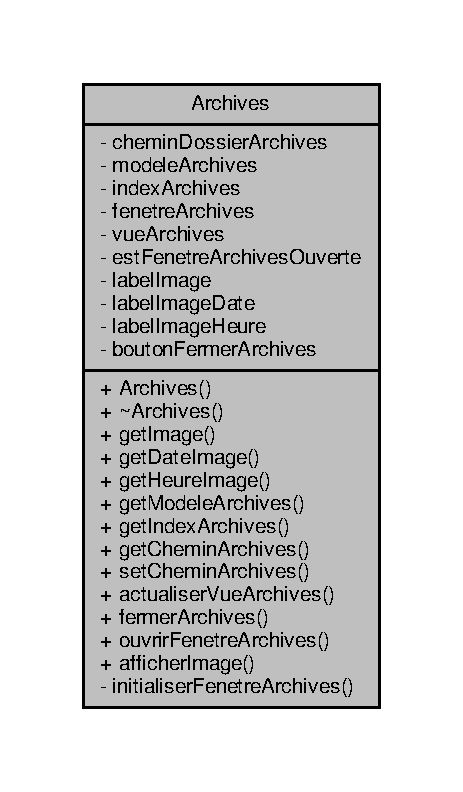
\includegraphics[width=222pt]{class_archives__coll__graph}
\end{center}
\end{figure}
\subsubsection*{Connecteurs publics}
\begin{DoxyCompactItemize}
\item 
void \hyperlink{class_archives_a0001d8b6a783f1f424965832e89a1f6f}{fermer\+Archives} ()
\begin{DoxyCompactList}\small\item\em Ferme la fenetre des archives. \end{DoxyCompactList}\item 
void \hyperlink{class_archives_a14d4f834ea05cf421161336607b4bb31}{ouvrir\+Fenetre\+Archives} ()
\begin{DoxyCompactList}\small\item\em Ouvre une fenetre menant aux archives des captures d\textquotesingle{}écrans. \end{DoxyCompactList}\item 
void \hyperlink{class_archives_a0e12a12774643d96831be4daba73976e}{afficher\+Image} (const Q\+Model\+Index \&\hyperlink{class_archives_a31cba52f3979585ee5e2b9390d21322b}{index\+Archives})
\begin{DoxyCompactList}\small\item\em Affiche l\textquotesingle{}image séléctionnée et les informations correspondantes. \end{DoxyCompactList}\end{DoxyCompactItemize}
\subsubsection*{Fonctions membres publiques}
\begin{DoxyCompactItemize}
\item 
\hyperlink{class_archives_ac30edd63c3f6c0df583bab7b9b9b4c76}{Archives} (Q\+Object $\ast$parent=nullptr)
\item 
\hyperlink{class_archives_a08c9ded9bb3da731991c5526dcdb2548}{$\sim$\+Archives} ()
\item 
Q\+String \hyperlink{class_archives_a9e35a0ff2d5823819cd2a9f8019c7b33}{get\+Image} (const Q\+Model\+Index \&\hyperlink{class_archives_a31cba52f3979585ee5e2b9390d21322b}{index\+Archives})
\begin{DoxyCompactList}\small\item\em Renvoie l\textquotesingle{}image des archives. \end{DoxyCompactList}\item 
Q\+String \hyperlink{class_archives_a5c1d731519acde8b59bc79973c4c1287}{get\+Date\+Image} (const Q\+Model\+Index \&\hyperlink{class_archives_a31cba52f3979585ee5e2b9390d21322b}{index\+Archives})
\begin{DoxyCompactList}\small\item\em Retourne la date de prise de l\textquotesingle{}image sélectionnée. \end{DoxyCompactList}\item 
Q\+String \hyperlink{class_archives_a91604a37aa9d4024ed79a71b12438003}{get\+Heure\+Image} (const Q\+Model\+Index \&\hyperlink{class_archives_a31cba52f3979585ee5e2b9390d21322b}{index\+Archives})
\begin{DoxyCompactList}\small\item\em Retourne l\textquotesingle{}heure de prise de l\textquotesingle{}image sélectionnée. \end{DoxyCompactList}\item 
Q\+File\+System\+Model $\ast$ \hyperlink{class_archives_ab5a55ac2e810cfdec3ce19af14087ceb}{get\+Modele\+Archives} ()
\begin{DoxyCompactList}\small\item\em Accesseur renvoyant le modèle de données. \end{DoxyCompactList}\item 
Q\+Model\+Index \hyperlink{class_archives_a3df83e6dd301afe331d7e75bd1b84a57}{get\+Index\+Archives} ()
\begin{DoxyCompactList}\small\item\em Accesseur renvoyant l\textquotesingle{}index du modèle de données. \end{DoxyCompactList}\item 
Q\+String \hyperlink{class_archives_a65dfbaba0123e6530b03bfb70e614c90}{get\+Chemin\+Archives} ()
\begin{DoxyCompactList}\small\item\em Accesseur renvoyant le chemin du dossier de stockage des photos. \end{DoxyCompactList}\item 
void \hyperlink{class_archives_a899e95a34c2a6f79b9a25355b5bf9cb6}{set\+Chemin\+Archives} (Q\+String nouveau\+Chemin\+Archives)
\begin{DoxyCompactList}\small\item\em Accesseur permettant de modifier le chemin vers les \hyperlink{class_archives}{Archives}. \end{DoxyCompactList}\item 
void \hyperlink{class_archives_a380ac387d773b07ea5138347dbaca65a}{actualiser\+Vue\+Archives} ()
\begin{DoxyCompactList}\small\item\em Actualise la vue des archives. \end{DoxyCompactList}\end{DoxyCompactItemize}
\subsubsection*{Fonctions membres privées}
\begin{DoxyCompactItemize}
\item 
void \hyperlink{class_archives_a1842ebad3721929949bc07be5144b79c}{initialiser\+Fenetre\+Archives} ()
\begin{DoxyCompactList}\small\item\em Initialise la fenetre pour naviguer dans les archives. \end{DoxyCompactList}\end{DoxyCompactItemize}
\subsubsection*{Attributs privés}
\begin{DoxyCompactItemize}
\item 
Q\+String \hyperlink{class_archives_af155e5062883030cddaa05623a34854b}{chemin\+Dossier\+Archives}
\begin{DoxyCompactList}\small\item\em le chemin du dossier de stockage des photos \end{DoxyCompactList}\item 
Q\+File\+System\+Model $\ast$ \hyperlink{class_archives_a61376e4ec330aea053fede230a1bc786}{modele\+Archives}
\begin{DoxyCompactList}\small\item\em le modèle de données \end{DoxyCompactList}\item 
Q\+Model\+Index \hyperlink{class_archives_a31cba52f3979585ee5e2b9390d21322b}{index\+Archives}
\begin{DoxyCompactList}\small\item\em l\textquotesingle{}index du modèle de données \end{DoxyCompactList}\item 
Q\+Dialog $\ast$ \hyperlink{class_archives_ad7c8209637b01f638b64530020d18b8e}{fenetre\+Archives}
\begin{DoxyCompactList}\small\item\em fenetre pour naviguer dans les archives \end{DoxyCompactList}\item 
Q\+List\+View $\ast$ \hyperlink{class_archives_a28fe566dcac396079d064460b17293b9}{vue\+Archives}
\begin{DoxyCompactList}\small\item\em la vue de la liste des archives \end{DoxyCompactList}\item 
bool \hyperlink{class_archives_a2b268dd292da50166988ad698af2b0fd}{est\+Fenetre\+Archives\+Ouverte}
\begin{DoxyCompactList}\small\item\em booléen indiquant si la fenêtre est ouverte \end{DoxyCompactList}\item 
Q\+Label $\ast$ \hyperlink{class_archives_af311679d957985d956a4ee5ad28a5988}{label\+Image}
\begin{DoxyCompactList}\small\item\em label pour l\textquotesingle{}affichage de la photo sélectionnée \end{DoxyCompactList}\item 
Q\+Label $\ast$ \hyperlink{class_archives_accb81477f1edca94691ae630ddc1f3f9}{label\+Image\+Date}
\begin{DoxyCompactList}\small\item\em label pour l\textquotesingle{}affichage de la date de la photo sélectionnée \end{DoxyCompactList}\item 
Q\+Label $\ast$ \hyperlink{class_archives_ab678af24ff4c67b8791ab52e998c79cb}{label\+Image\+Heure}
\begin{DoxyCompactList}\small\item\em label pour l\textquotesingle{}affichage de l\textquotesingle{}heure de la photo sélectionnée \end{DoxyCompactList}\item 
Q\+Push\+Button $\ast$ \hyperlink{class_archives_a598e607e203aee9386f85d55f20d8fda}{bouton\+Fermer\+Archives}
\begin{DoxyCompactList}\small\item\em bouton de fermeture de la fenêtre \end{DoxyCompactList}\end{DoxyCompactItemize}


\subsubsection{Description détaillée}
\begin{DoxyAuthor}{Auteur}
Nicolas B\+O\+F\+F\+R\+E\+DO
\end{DoxyAuthor}
\begin{DoxyVersion}{Version}
1.\+1
\end{DoxyVersion}
\begin{DoxyDate}{Date}
Mercredi 12 Juin 2019 
\end{DoxyDate}


\subsubsection{Documentation des constructeurs et destructeur}
\mbox{\Hypertarget{class_archives_ac30edd63c3f6c0df583bab7b9b9b4c76}\label{class_archives_ac30edd63c3f6c0df583bab7b9b9b4c76}} 
\index{Archives@{Archives}!Archives@{Archives}}
\index{Archives@{Archives}!Archives@{Archives}}
\paragraph{\texorpdfstring{Archives()}{Archives()}}
{\footnotesize\ttfamily Archives\+::\+Archives (\begin{DoxyParamCaption}\item[{Q\+Object $\ast$}]{parent = {\ttfamily nullptr} }\end{DoxyParamCaption})\hspace{0.3cm}{\ttfamily [explicit]}}

Constructeur de la classe \hyperlink{class_archives}{Archives} 
\begin{DoxyParams}{Paramètres}
{\em parent} & Q\+Object$\ast$ \\
\hline
\end{DoxyParams}


Références \hyperlink{class_archives_a1842ebad3721929949bc07be5144b79c}{initialiser\+Fenetre\+Archives()}.


\begin{DoxyCode}
00021                                   : QObject(parent), \hyperlink{class_archives_af155e5062883030cddaa05623a34854b}{cheminDossierArchives}(\textcolor{stringliteral}{" "}), 
      \hyperlink{class_archives_a61376e4ec330aea053fede230a1bc786}{modeleArchives}(\textcolor{keyword}{nullptr})
00022 \{
00023     \hyperlink{class_archives_a1842ebad3721929949bc07be5144b79c}{initialiserFenetreArchives}();
00024 \}
\end{DoxyCode}
\mbox{\Hypertarget{class_archives_a08c9ded9bb3da731991c5526dcdb2548}\label{class_archives_a08c9ded9bb3da731991c5526dcdb2548}} 
\index{Archives@{Archives}!````~Archives@{$\sim$\+Archives}}
\index{````~Archives@{$\sim$\+Archives}!Archives@{Archives}}
\paragraph{\texorpdfstring{$\sim$\+Archives()}{~Archives()}}
{\footnotesize\ttfamily Archives\+::$\sim$\+Archives (\begin{DoxyParamCaption}{ }\end{DoxyParamCaption})}

Destructeur de la classe \hyperlink{class_archives}{Archives} 
\begin{DoxyCode}
00031 \{
00032 \}
\end{DoxyCode}


\subsubsection{Documentation des fonctions membres}
\mbox{\Hypertarget{class_archives_a380ac387d773b07ea5138347dbaca65a}\label{class_archives_a380ac387d773b07ea5138347dbaca65a}} 
\index{Archives@{Archives}!actualiser\+Vue\+Archives@{actualiser\+Vue\+Archives}}
\index{actualiser\+Vue\+Archives@{actualiser\+Vue\+Archives}!Archives@{Archives}}
\paragraph{\texorpdfstring{actualiser\+Vue\+Archives()}{actualiserVueArchives()}}
{\footnotesize\ttfamily void Archives\+::actualiser\+Vue\+Archives (\begin{DoxyParamCaption}{ }\end{DoxyParamCaption})}

Est appellée à chaque fois que la fenêtre de navigation dans les archives est ouverte. 

Références \hyperlink{class_archives_a65dfbaba0123e6530b03bfb70e614c90}{get\+Chemin\+Archives()}, \hyperlink{class_archives_a3df83e6dd301afe331d7e75bd1b84a57}{get\+Index\+Archives()}, \hyperlink{class_archives_ab5a55ac2e810cfdec3ce19af14087ceb}{get\+Modele\+Archives()}, \hyperlink{class_archives_a31cba52f3979585ee5e2b9390d21322b}{index\+Archives}, \hyperlink{class_archives_a61376e4ec330aea053fede230a1bc786}{modele\+Archives}, et \hyperlink{class_archives_a28fe566dcac396079d064460b17293b9}{vue\+Archives}.



Référencé par \hyperlink{class_archives_a14d4f834ea05cf421161336607b4bb31}{ouvrir\+Fenetre\+Archives()}.


\begin{DoxyCode}
00186 \{
00187     \hyperlink{class_archives_a61376e4ec330aea053fede230a1bc786}{modeleArchives}->setRootPath(\hyperlink{class_archives_a65dfbaba0123e6530b03bfb70e614c90}{getCheminArchives}());
00188     \hyperlink{class_archives_a31cba52f3979585ee5e2b9390d21322b}{indexArchives} = \hyperlink{class_archives_a61376e4ec330aea053fede230a1bc786}{modeleArchives}->index(
      \hyperlink{class_archives_a65dfbaba0123e6530b03bfb70e614c90}{getCheminArchives}());
00189 
00190     \hyperlink{class_archives_a28fe566dcac396079d064460b17293b9}{vueArchives}->setModel(this->\hyperlink{class_archives_ab5a55ac2e810cfdec3ce19af14087ceb}{getModeleArchives}());
00191     \hyperlink{class_archives_a28fe566dcac396079d064460b17293b9}{vueArchives}->setRootIndex(this->\hyperlink{class_archives_a3df83e6dd301afe331d7e75bd1b84a57}{getIndexArchives}());
00192 \}
\end{DoxyCode}
\mbox{\Hypertarget{class_archives_a0e12a12774643d96831be4daba73976e}\label{class_archives_a0e12a12774643d96831be4daba73976e}} 
\index{Archives@{Archives}!afficher\+Image@{afficher\+Image}}
\index{afficher\+Image@{afficher\+Image}!Archives@{Archives}}
\paragraph{\texorpdfstring{afficher\+Image}{afficherImage}}
{\footnotesize\ttfamily void Archives\+::afficher\+Image (\begin{DoxyParamCaption}\item[{const Q\+Model\+Index \&}]{index\+Archives }\end{DoxyParamCaption})\hspace{0.3cm}{\ttfamily [slot]}}


\begin{DoxyParams}{Paramètres}
{\em index\+Archives} & Q\+Model\+Index \\
\hline
\end{DoxyParams}


Références \hyperlink{class_archives_a5c1d731519acde8b59bc79973c4c1287}{get\+Date\+Image()}, \hyperlink{class_archives_a91604a37aa9d4024ed79a71b12438003}{get\+Heure\+Image()}, \hyperlink{class_archives_a9e35a0ff2d5823819cd2a9f8019c7b33}{get\+Image()}, \hyperlink{class_archives_af311679d957985d956a4ee5ad28a5988}{label\+Image}, \hyperlink{class_archives_accb81477f1edca94691ae630ddc1f3f9}{label\+Image\+Date}, et \hyperlink{class_archives_ab678af24ff4c67b8791ab52e998c79cb}{label\+Image\+Heure}.



Référencé par \hyperlink{class_archives_a1842ebad3721929949bc07be5144b79c}{initialiser\+Fenetre\+Archives()}.


\begin{DoxyCode}
00210 \{
00211     \hyperlink{class_archives_af311679d957985d956a4ee5ad28a5988}{labelImage}->setPixmap(QPixmap(this->\hyperlink{class_archives_a9e35a0ff2d5823819cd2a9f8019c7b33}{getImage}(\hyperlink{class_archives_a31cba52f3979585ee5e2b9390d21322b}{indexArchives})));
00212     \hyperlink{class_archives_af311679d957985d956a4ee5ad28a5988}{labelImage}->setScaledContents(\textcolor{keyword}{true});
00213     \hyperlink{class_archives_accb81477f1edca94691ae630ddc1f3f9}{labelImageDate}->setText(\textcolor{stringliteral}{"Date : "} + this->\hyperlink{class_archives_a5c1d731519acde8b59bc79973c4c1287}{getDateImage}(
      \hyperlink{class_archives_a31cba52f3979585ee5e2b9390d21322b}{indexArchives}));
00214     \hyperlink{class_archives_ab678af24ff4c67b8791ab52e998c79cb}{labelImageHeure}->setText(\textcolor{stringliteral}{"Heure : "} + this->\hyperlink{class_archives_a91604a37aa9d4024ed79a71b12438003}{getHeureImage}(
      \hyperlink{class_archives_a31cba52f3979585ee5e2b9390d21322b}{indexArchives}));
00215 \}
\end{DoxyCode}
\mbox{\Hypertarget{class_archives_a0001d8b6a783f1f424965832e89a1f6f}\label{class_archives_a0001d8b6a783f1f424965832e89a1f6f}} 
\index{Archives@{Archives}!fermer\+Archives@{fermer\+Archives}}
\index{fermer\+Archives@{fermer\+Archives}!Archives@{Archives}}
\paragraph{\texorpdfstring{fermer\+Archives}{fermerArchives}}
{\footnotesize\ttfamily void Archives\+::fermer\+Archives (\begin{DoxyParamCaption}{ }\end{DoxyParamCaption})\hspace{0.3cm}{\ttfamily [slot]}}



Références \hyperlink{class_archives_ad7c8209637b01f638b64530020d18b8e}{fenetre\+Archives}.



Référencé par \hyperlink{class_archives_a1842ebad3721929949bc07be5144b79c}{initialiser\+Fenetre\+Archives()}.


\begin{DoxyCode}
00222 \{
00223     \hyperlink{class_archives_ad7c8209637b01f638b64530020d18b8e}{fenetreArchives}->close();
00224 \}
\end{DoxyCode}
\mbox{\Hypertarget{class_archives_a65dfbaba0123e6530b03bfb70e614c90}\label{class_archives_a65dfbaba0123e6530b03bfb70e614c90}} 
\index{Archives@{Archives}!get\+Chemin\+Archives@{get\+Chemin\+Archives}}
\index{get\+Chemin\+Archives@{get\+Chemin\+Archives}!Archives@{Archives}}
\paragraph{\texorpdfstring{get\+Chemin\+Archives()}{getCheminArchives()}}
{\footnotesize\ttfamily Q\+String Archives\+::get\+Chemin\+Archives (\begin{DoxyParamCaption}{ }\end{DoxyParamCaption})}

\begin{DoxyReturn}{Renvoie}
Un {\itshape Q\+String} indiquant le chemin du dossier de stockage des photos. 
\end{DoxyReturn}


Références \hyperlink{class_archives_af155e5062883030cddaa05623a34854b}{chemin\+Dossier\+Archives}.



Référencé par \hyperlink{class_archives_a380ac387d773b07ea5138347dbaca65a}{actualiser\+Vue\+Archives()}, \hyperlink{class_rov_ae1306036b067e9ad50a09f9dd607a092}{Rov\+::creer\+Nouvelle\+Campagne()}, \hyperlink{class_archives_a9e35a0ff2d5823819cd2a9f8019c7b33}{get\+Image()}, \hyperlink{class_archives_a1842ebad3721929949bc07be5144b79c}{initialiser\+Fenetre\+Archives()}, et \hyperlink{class_camera_a60d2c9f16b6f235ab6dd0360c883e0d0}{Camera\+::nommer\+Capture()}.


\begin{DoxyCode}
00040 \{
00041     qDebug() << Q\_FUNC\_INFO;
00042     \textcolor{keywordflow}{return} \hyperlink{class_archives_af155e5062883030cddaa05623a34854b}{cheminDossierArchives};
00043 \}
\end{DoxyCode}
\mbox{\Hypertarget{class_archives_a5c1d731519acde8b59bc79973c4c1287}\label{class_archives_a5c1d731519acde8b59bc79973c4c1287}} 
\index{Archives@{Archives}!get\+Date\+Image@{get\+Date\+Image}}
\index{get\+Date\+Image@{get\+Date\+Image}!Archives@{Archives}}
\paragraph{\texorpdfstring{get\+Date\+Image()}{getDateImage()}}
{\footnotesize\ttfamily Q\+String Archives\+::get\+Date\+Image (\begin{DoxyParamCaption}\item[{const Q\+Model\+Index \&}]{index\+Archives }\end{DoxyParamCaption})}


\begin{DoxyParams}{Paramètres}
{\em index\+Archives} & const Q\+Model\+Index \&, L\textquotesingle{}index de l\textquotesingle{}image des archives \\
\hline
\end{DoxyParams}
\begin{DoxyReturn}{Renvoie}
Un {\itshape Q\+String} indiquant la date de prise de l\textquotesingle{}image sélectionnée 
\end{DoxyReturn}


Référencé par \hyperlink{class_archives_a0e12a12774643d96831be4daba73976e}{afficher\+Image()}.


\begin{DoxyCode}
00096 \{
00097     QString dateImage = \hyperlink{class_archives_a31cba52f3979585ee5e2b9390d21322b}{indexArchives}.data().toString().left(10);
00098     QStringList mois;
00099 
00100     dateImage.replace(2, 1, \textcolor{stringliteral}{" "});
00101     dateImage.replace(5, 1, \textcolor{stringliteral}{" "});
00102 
00103     mois << QString::fromUtf8(\textcolor{stringliteral}{"Janvier"}) << QString::fromUtf8(\textcolor{stringliteral}{"Février"}) << QString::fromUtf8(\textcolor{stringliteral}{"Mars"}) << 
      QString::fromUtf8(\textcolor{stringliteral}{"Avril"}) << QString::fromUtf8(\textcolor{stringliteral}{"Mai"}) << QString::fromUtf8(\textcolor{stringliteral}{"Juin"}) << QString::fromUtf8(\textcolor{stringliteral}{"
      Juillet"}) << QString::fromUtf8(\textcolor{stringliteral}{"Août"}) << QString::fromUtf8(\textcolor{stringliteral}{"Septembre"}) << QString::fromUtf8(\textcolor{stringliteral}{"Octobre"}) << 
      QString::fromUtf8(\textcolor{stringliteral}{"Novembre"}) << QString::fromUtf8(\textcolor{stringliteral}{"Décembre"});
00104     dateImage.replace(3, 2, mois.at(dateImage.left(5).right(3).toInt() - 1));
00105 
00106     \textcolor{keywordflow}{return} dateImage;
00107 \}
\end{DoxyCode}
\mbox{\Hypertarget{class_archives_a91604a37aa9d4024ed79a71b12438003}\label{class_archives_a91604a37aa9d4024ed79a71b12438003}} 
\index{Archives@{Archives}!get\+Heure\+Image@{get\+Heure\+Image}}
\index{get\+Heure\+Image@{get\+Heure\+Image}!Archives@{Archives}}
\paragraph{\texorpdfstring{get\+Heure\+Image()}{getHeureImage()}}
{\footnotesize\ttfamily Q\+String Archives\+::get\+Heure\+Image (\begin{DoxyParamCaption}\item[{const Q\+Model\+Index \&}]{index\+Archives }\end{DoxyParamCaption})}


\begin{DoxyParams}{Paramètres}
{\em index\+Archives} & const Q\+Model\+Index \&, L\textquotesingle{}index de l\textquotesingle{}images des archives \\
\hline
\end{DoxyParams}
\begin{DoxyReturn}{Renvoie}
Un {\itshape Q\+String} indiquant l\textquotesingle{}heure de prise de l\textquotesingle{}image sélectionnée 
\end{DoxyReturn}


Référencé par \hyperlink{class_archives_a0e12a12774643d96831be4daba73976e}{afficher\+Image()}.


\begin{DoxyCode}
00116 \{
00117     QString heureImage = \hyperlink{class_archives_a31cba52f3979585ee5e2b9390d21322b}{indexArchives}.data().toString().remove(19, 4).right(8);
00118     heureImage.replace(2, 1, \textcolor{stringliteral}{"h "});
00119     heureImage.replace(6, 1, \textcolor{stringliteral}{"m "});
00120     heureImage.append(\textcolor{charliteral}{'s'});
00121 
00122     \textcolor{keywordflow}{return} heureImage;
00123 \}
\end{DoxyCode}
\mbox{\Hypertarget{class_archives_a9e35a0ff2d5823819cd2a9f8019c7b33}\label{class_archives_a9e35a0ff2d5823819cd2a9f8019c7b33}} 
\index{Archives@{Archives}!get\+Image@{get\+Image}}
\index{get\+Image@{get\+Image}!Archives@{Archives}}
\paragraph{\texorpdfstring{get\+Image()}{getImage()}}
{\footnotesize\ttfamily Q\+String Archives\+::get\+Image (\begin{DoxyParamCaption}\item[{const Q\+Model\+Index \&}]{index\+Archives }\end{DoxyParamCaption})}


\begin{DoxyParams}{Paramètres}
{\em index\+Archives} & Q\+Model\+Index \& index sur le modèle des fichiers contenus dans le Q\+List\+View \\
\hline
\end{DoxyParams}
\begin{DoxyReturn}{Renvoie}
un {\itshape Q\+String} indiquant le nom de l\textquotesingle{}image 
\end{DoxyReturn}


Références \hyperlink{class_archives_a65dfbaba0123e6530b03bfb70e614c90}{get\+Chemin\+Archives()}.



Référencé par \hyperlink{class_archives_a0e12a12774643d96831be4daba73976e}{afficher\+Image()}.


\begin{DoxyCode}
00063 \{
00064     QString cheminImage = \hyperlink{class_archives_a65dfbaba0123e6530b03bfb70e614c90}{getCheminArchives}() + \hyperlink{class_archives_a31cba52f3979585ee5e2b9390d21322b}{indexArchives}.data().toString
      ();
00065     qDebug() << Q\_FUNC\_INFO << \textcolor{stringliteral}{"cheminImage"} << cheminImage;
00066     \textcolor{keywordflow}{return} cheminImage;
00067 \}
\end{DoxyCode}
\mbox{\Hypertarget{class_archives_a3df83e6dd301afe331d7e75bd1b84a57}\label{class_archives_a3df83e6dd301afe331d7e75bd1b84a57}} 
\index{Archives@{Archives}!get\+Index\+Archives@{get\+Index\+Archives}}
\index{get\+Index\+Archives@{get\+Index\+Archives}!Archives@{Archives}}
\paragraph{\texorpdfstring{get\+Index\+Archives()}{getIndexArchives()}}
{\footnotesize\ttfamily Q\+Model\+Index Archives\+::get\+Index\+Archives (\begin{DoxyParamCaption}{ }\end{DoxyParamCaption})}

\begin{DoxyReturn}{Renvoie}
Un {\itshape Q\+Model\+Index} indiquant l\textquotesingle{}index du modèle de données. 
\end{DoxyReturn}


Références \hyperlink{class_archives_a31cba52f3979585ee5e2b9390d21322b}{index\+Archives}.



Référencé par \hyperlink{class_archives_a380ac387d773b07ea5138347dbaca65a}{actualiser\+Vue\+Archives()}, et \hyperlink{class_archives_a1842ebad3721929949bc07be5144b79c}{initialiser\+Fenetre\+Archives()}.


\begin{DoxyCode}
00085 \{
00086     \textcolor{keywordflow}{return} \hyperlink{class_archives_a31cba52f3979585ee5e2b9390d21322b}{indexArchives};
00087 \}
\end{DoxyCode}
\mbox{\Hypertarget{class_archives_ab5a55ac2e810cfdec3ce19af14087ceb}\label{class_archives_ab5a55ac2e810cfdec3ce19af14087ceb}} 
\index{Archives@{Archives}!get\+Modele\+Archives@{get\+Modele\+Archives}}
\index{get\+Modele\+Archives@{get\+Modele\+Archives}!Archives@{Archives}}
\paragraph{\texorpdfstring{get\+Modele\+Archives()}{getModeleArchives()}}
{\footnotesize\ttfamily Q\+File\+System\+Model $\ast$ Archives\+::get\+Modele\+Archives (\begin{DoxyParamCaption}{ }\end{DoxyParamCaption})}

\begin{DoxyReturn}{Renvoie}
Un {\itshape Q\+File\+System\+Model$\ast$} indiquant le modèle de données. 
\end{DoxyReturn}


Références \hyperlink{class_archives_a61376e4ec330aea053fede230a1bc786}{modele\+Archives}.



Référencé par \hyperlink{class_archives_a380ac387d773b07ea5138347dbaca65a}{actualiser\+Vue\+Archives()}, et \hyperlink{class_archives_a1842ebad3721929949bc07be5144b79c}{initialiser\+Fenetre\+Archives()}.


\begin{DoxyCode}
00075 \{
00076     \textcolor{keywordflow}{return} \hyperlink{class_archives_a61376e4ec330aea053fede230a1bc786}{modeleArchives};
00077 \}
\end{DoxyCode}
\mbox{\Hypertarget{class_archives_a1842ebad3721929949bc07be5144b79c}\label{class_archives_a1842ebad3721929949bc07be5144b79c}} 
\index{Archives@{Archives}!initialiser\+Fenetre\+Archives@{initialiser\+Fenetre\+Archives}}
\index{initialiser\+Fenetre\+Archives@{initialiser\+Fenetre\+Archives}!Archives@{Archives}}
\paragraph{\texorpdfstring{initialiser\+Fenetre\+Archives()}{initialiserFenetreArchives()}}
{\footnotesize\ttfamily void Archives\+::initialiser\+Fenetre\+Archives (\begin{DoxyParamCaption}{ }\end{DoxyParamCaption})\hspace{0.3cm}{\ttfamily [private]}}

La taille de la fenetre est fixer en fonction de la resolution des photos prises. 

Références \hyperlink{class_archives_a0e12a12774643d96831be4daba73976e}{afficher\+Image()}, \hyperlink{class_archives_a598e607e203aee9386f85d55f20d8fda}{bouton\+Fermer\+Archives}, \hyperlink{class_archives_ad7c8209637b01f638b64530020d18b8e}{fenetre\+Archives}, \hyperlink{class_archives_a0001d8b6a783f1f424965832e89a1f6f}{fermer\+Archives()}, \hyperlink{class_archives_a65dfbaba0123e6530b03bfb70e614c90}{get\+Chemin\+Archives()}, \hyperlink{class_archives_a3df83e6dd301afe331d7e75bd1b84a57}{get\+Index\+Archives()}, \hyperlink{class_archives_ab5a55ac2e810cfdec3ce19af14087ceb}{get\+Modele\+Archives()}, \hyperlink{class_archives_a31cba52f3979585ee5e2b9390d21322b}{index\+Archives}, \hyperlink{class_archives_af311679d957985d956a4ee5ad28a5988}{label\+Image}, \hyperlink{class_archives_accb81477f1edca94691ae630ddc1f3f9}{label\+Image\+Date}, \hyperlink{class_archives_ab678af24ff4c67b8791ab52e998c79cb}{label\+Image\+Heure}, \hyperlink{class_archives_a61376e4ec330aea053fede230a1bc786}{modele\+Archives}, et \hyperlink{class_archives_a28fe566dcac396079d064460b17293b9}{vue\+Archives}.



Référencé par \hyperlink{class_archives_ac30edd63c3f6c0df583bab7b9b9b4c76}{Archives()}.


\begin{DoxyCode}
00131 \{
00132     \hyperlink{class_archives_a61376e4ec330aea053fede230a1bc786}{modeleArchives} = \textcolor{keyword}{new} QFileSystemModel;
00133     \hyperlink{class_archives_a61376e4ec330aea053fede230a1bc786}{modeleArchives}->setRootPath(\hyperlink{class_archives_a65dfbaba0123e6530b03bfb70e614c90}{getCheminArchives}());
00134     \hyperlink{class_archives_a31cba52f3979585ee5e2b9390d21322b}{indexArchives} = \hyperlink{class_archives_a61376e4ec330aea053fede230a1bc786}{modeleArchives}->index(
      \hyperlink{class_archives_a65dfbaba0123e6530b03bfb70e614c90}{getCheminArchives}());
00135 
00136     \hyperlink{class_archives_ad7c8209637b01f638b64530020d18b8e}{fenetreArchives} = \textcolor{keyword}{new} QDialog();
00137     \hyperlink{class_archives_a28fe566dcac396079d064460b17293b9}{vueArchives} = \textcolor{keyword}{new} QListView;
00138     \hyperlink{class_archives_af311679d957985d956a4ee5ad28a5988}{labelImage} = \textcolor{keyword}{new} QLabel;
00139     \hyperlink{class_archives_accb81477f1edca94691ae630ddc1f3f9}{labelImageDate} = \textcolor{keyword}{new} QLabel;
00140     \hyperlink{class_archives_ab678af24ff4c67b8791ab52e998c79cb}{labelImageHeure} = \textcolor{keyword}{new} QLabel;
00141     \hyperlink{class_archives_a598e607e203aee9386f85d55f20d8fda}{boutonFermerArchives} = \textcolor{keyword}{new} QPushButton(\textcolor{stringliteral}{"&Fermer"});
00142 
00143     \textcolor{keyword}{const} \textcolor{keywordtype}{int} hauteurImage = 480;
00144     \textcolor{keyword}{const} \textcolor{keywordtype}{int} largeurImage = 640;
00145     \textcolor{keyword}{const} \textcolor{keywordtype}{int} hauteurInformations = (hauteurImage/10);
00146     \textcolor{keyword}{const} \textcolor{keywordtype}{int} largeurMAX = largeurImage + largeurImage/2;
00147     \textcolor{keyword}{const} \textcolor{keywordtype}{int} hauteurMAX = hauteurImage + hauteurInformations;
00148 
00149     \hyperlink{class_archives_a28fe566dcac396079d064460b17293b9}{vueArchives}->setModel(this->\hyperlink{class_archives_ab5a55ac2e810cfdec3ce19af14087ceb}{getModeleArchives}());
00150     \hyperlink{class_archives_a28fe566dcac396079d064460b17293b9}{vueArchives}->setRootIndex(this->\hyperlink{class_archives_a3df83e6dd301afe331d7e75bd1b84a57}{getIndexArchives}());
00151 
00152     QHBoxLayout *hLayoutPrincipalArchives = \textcolor{keyword}{new} QHBoxLayout;
00153     QVBoxLayout *vLayoutSelections = \textcolor{keyword}{new} QVBoxLayout;
00154     QVBoxLayout *vLayoutImage = \textcolor{keyword}{new} QVBoxLayout;
00155     QHBoxLayout *hLayoutInformationsImage = \textcolor{keyword}{new} QHBoxLayout;
00156 
00157     hLayoutPrincipalArchives->addLayout(vLayoutImage);
00158     hLayoutPrincipalArchives->addLayout(vLayoutSelections);
00159     vLayoutSelections->addWidget(\hyperlink{class_archives_a28fe566dcac396079d064460b17293b9}{vueArchives});
00160     vLayoutSelections->addWidget(\hyperlink{class_archives_a598e607e203aee9386f85d55f20d8fda}{boutonFermerArchives});
00161     vLayoutImage->addLayout(hLayoutInformationsImage);
00162     vLayoutImage->addWidget(\hyperlink{class_archives_af311679d957985d956a4ee5ad28a5988}{labelImage});
00163     hLayoutInformationsImage->addWidget(\hyperlink{class_archives_accb81477f1edca94691ae630ddc1f3f9}{labelImageDate});
00164     hLayoutInformationsImage->addWidget(\hyperlink{class_archives_ab678af24ff4c67b8791ab52e998c79cb}{labelImageHeure});
00165 
00166     \hyperlink{class_archives_ad7c8209637b01f638b64530020d18b8e}{fenetreArchives}->setWindowTitle(\textcolor{stringliteral}{"Archives Photo"});
00167     \hyperlink{class_archives_ad7c8209637b01f638b64530020d18b8e}{fenetreArchives}->setFixedSize(largeurMAX, hauteurMAX);
00168     \hyperlink{class_archives_ad7c8209637b01f638b64530020d18b8e}{fenetreArchives}->setLayout(hLayoutPrincipalArchives);
00169     \hyperlink{class_archives_af311679d957985d956a4ee5ad28a5988}{labelImage}->setFixedHeight(hauteurImage);
00170     \hyperlink{class_archives_af311679d957985d956a4ee5ad28a5988}{labelImage}->setFixedWidth(largeurImage);
00171     \hyperlink{class_archives_accb81477f1edca94691ae630ddc1f3f9}{labelImageDate}->setFixedHeight(hauteurInformations);
00172     \hyperlink{class_archives_ab678af24ff4c67b8791ab52e998c79cb}{labelImageHeure}->setFixedHeight(hauteurInformations);
00173 
00174     connect(\hyperlink{class_archives_a28fe566dcac396079d064460b17293b9}{vueArchives}, SIGNAL(doubleClicked(\textcolor{keyword}{const} QModelIndex)), \textcolor{keyword}{this}, SLOT(
      \hyperlink{class_archives_a0e12a12774643d96831be4daba73976e}{afficherImage}(\textcolor{keyword}{const} QModelIndex)));
00175     connect(\hyperlink{class_archives_a598e607e203aee9386f85d55f20d8fda}{boutonFermerArchives}, SIGNAL(clicked()), \textcolor{keyword}{this}, SLOT(
      \hyperlink{class_archives_a0001d8b6a783f1f424965832e89a1f6f}{fermerArchives}()));
00176 
00177     \hyperlink{class_archives_ad7c8209637b01f638b64530020d18b8e}{fenetreArchives}->setWindowFlags(Qt::Dialog | Qt::WindowCloseButtonHint);
00178 \}
\end{DoxyCode}
\mbox{\Hypertarget{class_archives_a14d4f834ea05cf421161336607b4bb31}\label{class_archives_a14d4f834ea05cf421161336607b4bb31}} 
\index{Archives@{Archives}!ouvrir\+Fenetre\+Archives@{ouvrir\+Fenetre\+Archives}}
\index{ouvrir\+Fenetre\+Archives@{ouvrir\+Fenetre\+Archives}!Archives@{Archives}}
\paragraph{\texorpdfstring{ouvrir\+Fenetre\+Archives}{ouvrirFenetreArchives}}
{\footnotesize\ttfamily void Archives\+::ouvrir\+Fenetre\+Archives (\begin{DoxyParamCaption}{ }\end{DoxyParamCaption})\hspace{0.3cm}{\ttfamily [slot]}}



Références \hyperlink{class_archives_a380ac387d773b07ea5138347dbaca65a}{actualiser\+Vue\+Archives()}, et \hyperlink{class_archives_ad7c8209637b01f638b64530020d18b8e}{fenetre\+Archives}.


\begin{DoxyCode}
00199 \{
00200     \hyperlink{class_archives_a380ac387d773b07ea5138347dbaca65a}{actualiserVueArchives}();
00201     \hyperlink{class_archives_ad7c8209637b01f638b64530020d18b8e}{fenetreArchives}->exec();
00202 \}
\end{DoxyCode}
\mbox{\Hypertarget{class_archives_a899e95a34c2a6f79b9a25355b5bf9cb6}\label{class_archives_a899e95a34c2a6f79b9a25355b5bf9cb6}} 
\index{Archives@{Archives}!set\+Chemin\+Archives@{set\+Chemin\+Archives}}
\index{set\+Chemin\+Archives@{set\+Chemin\+Archives}!Archives@{Archives}}
\paragraph{\texorpdfstring{set\+Chemin\+Archives()}{setCheminArchives()}}
{\footnotesize\ttfamily void Archives\+::set\+Chemin\+Archives (\begin{DoxyParamCaption}\item[{Q\+String}]{nouveau\+Chemin\+Archives }\end{DoxyParamCaption})}


\begin{DoxyParams}{Paramètres}
{\em nouveau\+Chemin\+Archives} & Q\+String le nouveau chemin des \hyperlink{class_archives}{Archives}. \\
\hline
\end{DoxyParams}


Références \hyperlink{class_archives_af155e5062883030cddaa05623a34854b}{chemin\+Dossier\+Archives}.



Référencé par \hyperlink{class_rov_a53f656be57fa1eb7b93e03095a597439}{Rov\+::creer\+Dossier\+Archives()}.


\begin{DoxyCode}
00051 \{
00052     qDebug() << Q\_FUNC\_INFO << nouveauCheminArchives;
00053     \hyperlink{class_archives_af155e5062883030cddaa05623a34854b}{cheminDossierArchives} = nouveauCheminArchives;
00054 \}
\end{DoxyCode}


\subsubsection{Documentation des données membres}
\mbox{\Hypertarget{class_archives_a598e607e203aee9386f85d55f20d8fda}\label{class_archives_a598e607e203aee9386f85d55f20d8fda}} 
\index{Archives@{Archives}!bouton\+Fermer\+Archives@{bouton\+Fermer\+Archives}}
\index{bouton\+Fermer\+Archives@{bouton\+Fermer\+Archives}!Archives@{Archives}}
\paragraph{\texorpdfstring{bouton\+Fermer\+Archives}{boutonFermerArchives}}
{\footnotesize\ttfamily Q\+Push\+Button$\ast$ Archives\+::bouton\+Fermer\+Archives\hspace{0.3cm}{\ttfamily [private]}}



Référencé par \hyperlink{class_archives_a1842ebad3721929949bc07be5144b79c}{initialiser\+Fenetre\+Archives()}.

\mbox{\Hypertarget{class_archives_af155e5062883030cddaa05623a34854b}\label{class_archives_af155e5062883030cddaa05623a34854b}} 
\index{Archives@{Archives}!chemin\+Dossier\+Archives@{chemin\+Dossier\+Archives}}
\index{chemin\+Dossier\+Archives@{chemin\+Dossier\+Archives}!Archives@{Archives}}
\paragraph{\texorpdfstring{chemin\+Dossier\+Archives}{cheminDossierArchives}}
{\footnotesize\ttfamily Q\+String Archives\+::chemin\+Dossier\+Archives\hspace{0.3cm}{\ttfamily [private]}}



Référencé par \hyperlink{class_archives_a65dfbaba0123e6530b03bfb70e614c90}{get\+Chemin\+Archives()}, et \hyperlink{class_archives_a899e95a34c2a6f79b9a25355b5bf9cb6}{set\+Chemin\+Archives()}.

\mbox{\Hypertarget{class_archives_a2b268dd292da50166988ad698af2b0fd}\label{class_archives_a2b268dd292da50166988ad698af2b0fd}} 
\index{Archives@{Archives}!est\+Fenetre\+Archives\+Ouverte@{est\+Fenetre\+Archives\+Ouverte}}
\index{est\+Fenetre\+Archives\+Ouverte@{est\+Fenetre\+Archives\+Ouverte}!Archives@{Archives}}
\paragraph{\texorpdfstring{est\+Fenetre\+Archives\+Ouverte}{estFenetreArchivesOuverte}}
{\footnotesize\ttfamily bool Archives\+::est\+Fenetre\+Archives\+Ouverte\hspace{0.3cm}{\ttfamily [private]}}

\mbox{\Hypertarget{class_archives_ad7c8209637b01f638b64530020d18b8e}\label{class_archives_ad7c8209637b01f638b64530020d18b8e}} 
\index{Archives@{Archives}!fenetre\+Archives@{fenetre\+Archives}}
\index{fenetre\+Archives@{fenetre\+Archives}!Archives@{Archives}}
\paragraph{\texorpdfstring{fenetre\+Archives}{fenetreArchives}}
{\footnotesize\ttfamily Q\+Dialog$\ast$ Archives\+::fenetre\+Archives\hspace{0.3cm}{\ttfamily [private]}}



Référencé par \hyperlink{class_archives_a0001d8b6a783f1f424965832e89a1f6f}{fermer\+Archives()}, \hyperlink{class_archives_a1842ebad3721929949bc07be5144b79c}{initialiser\+Fenetre\+Archives()}, et \hyperlink{class_archives_a14d4f834ea05cf421161336607b4bb31}{ouvrir\+Fenetre\+Archives()}.

\mbox{\Hypertarget{class_archives_a31cba52f3979585ee5e2b9390d21322b}\label{class_archives_a31cba52f3979585ee5e2b9390d21322b}} 
\index{Archives@{Archives}!index\+Archives@{index\+Archives}}
\index{index\+Archives@{index\+Archives}!Archives@{Archives}}
\paragraph{\texorpdfstring{index\+Archives}{indexArchives}}
{\footnotesize\ttfamily Q\+Model\+Index Archives\+::index\+Archives\hspace{0.3cm}{\ttfamily [private]}}



Référencé par \hyperlink{class_archives_a380ac387d773b07ea5138347dbaca65a}{actualiser\+Vue\+Archives()}, \hyperlink{class_archives_a3df83e6dd301afe331d7e75bd1b84a57}{get\+Index\+Archives()}, et \hyperlink{class_archives_a1842ebad3721929949bc07be5144b79c}{initialiser\+Fenetre\+Archives()}.

\mbox{\Hypertarget{class_archives_af311679d957985d956a4ee5ad28a5988}\label{class_archives_af311679d957985d956a4ee5ad28a5988}} 
\index{Archives@{Archives}!label\+Image@{label\+Image}}
\index{label\+Image@{label\+Image}!Archives@{Archives}}
\paragraph{\texorpdfstring{label\+Image}{labelImage}}
{\footnotesize\ttfamily Q\+Label$\ast$ Archives\+::label\+Image\hspace{0.3cm}{\ttfamily [private]}}



Référencé par \hyperlink{class_archives_a0e12a12774643d96831be4daba73976e}{afficher\+Image()}, et \hyperlink{class_archives_a1842ebad3721929949bc07be5144b79c}{initialiser\+Fenetre\+Archives()}.

\mbox{\Hypertarget{class_archives_accb81477f1edca94691ae630ddc1f3f9}\label{class_archives_accb81477f1edca94691ae630ddc1f3f9}} 
\index{Archives@{Archives}!label\+Image\+Date@{label\+Image\+Date}}
\index{label\+Image\+Date@{label\+Image\+Date}!Archives@{Archives}}
\paragraph{\texorpdfstring{label\+Image\+Date}{labelImageDate}}
{\footnotesize\ttfamily Q\+Label$\ast$ Archives\+::label\+Image\+Date\hspace{0.3cm}{\ttfamily [private]}}



Référencé par \hyperlink{class_archives_a0e12a12774643d96831be4daba73976e}{afficher\+Image()}, et \hyperlink{class_archives_a1842ebad3721929949bc07be5144b79c}{initialiser\+Fenetre\+Archives()}.

\mbox{\Hypertarget{class_archives_ab678af24ff4c67b8791ab52e998c79cb}\label{class_archives_ab678af24ff4c67b8791ab52e998c79cb}} 
\index{Archives@{Archives}!label\+Image\+Heure@{label\+Image\+Heure}}
\index{label\+Image\+Heure@{label\+Image\+Heure}!Archives@{Archives}}
\paragraph{\texorpdfstring{label\+Image\+Heure}{labelImageHeure}}
{\footnotesize\ttfamily Q\+Label$\ast$ Archives\+::label\+Image\+Heure\hspace{0.3cm}{\ttfamily [private]}}



Référencé par \hyperlink{class_archives_a0e12a12774643d96831be4daba73976e}{afficher\+Image()}, et \hyperlink{class_archives_a1842ebad3721929949bc07be5144b79c}{initialiser\+Fenetre\+Archives()}.

\mbox{\Hypertarget{class_archives_a61376e4ec330aea053fede230a1bc786}\label{class_archives_a61376e4ec330aea053fede230a1bc786}} 
\index{Archives@{Archives}!modele\+Archives@{modele\+Archives}}
\index{modele\+Archives@{modele\+Archives}!Archives@{Archives}}
\paragraph{\texorpdfstring{modele\+Archives}{modeleArchives}}
{\footnotesize\ttfamily Q\+File\+System\+Model$\ast$ Archives\+::modele\+Archives\hspace{0.3cm}{\ttfamily [private]}}



Référencé par \hyperlink{class_archives_a380ac387d773b07ea5138347dbaca65a}{actualiser\+Vue\+Archives()}, \hyperlink{class_archives_ab5a55ac2e810cfdec3ce19af14087ceb}{get\+Modele\+Archives()}, et \hyperlink{class_archives_a1842ebad3721929949bc07be5144b79c}{initialiser\+Fenetre\+Archives()}.

\mbox{\Hypertarget{class_archives_a28fe566dcac396079d064460b17293b9}\label{class_archives_a28fe566dcac396079d064460b17293b9}} 
\index{Archives@{Archives}!vue\+Archives@{vue\+Archives}}
\index{vue\+Archives@{vue\+Archives}!Archives@{Archives}}
\paragraph{\texorpdfstring{vue\+Archives}{vueArchives}}
{\footnotesize\ttfamily Q\+List\+View$\ast$ Archives\+::vue\+Archives\hspace{0.3cm}{\ttfamily [private]}}



Référencé par \hyperlink{class_archives_a380ac387d773b07ea5138347dbaca65a}{actualiser\+Vue\+Archives()}, et \hyperlink{class_archives_a1842ebad3721929949bc07be5144b79c}{initialiser\+Fenetre\+Archives()}.



La documentation de cette classe a été générée à partir des fichiers suivants \+:\begin{DoxyCompactItemize}
\item 
\hyperlink{archives_8h}{archives.\+h}\item 
\hyperlink{archives_8cpp}{archives.\+cpp}\end{DoxyCompactItemize}

\hypertarget{class_base_de_donnees}{}\subsection{Référence de la classe Base\+De\+Donnees}
\label{class_base_de_donnees}\index{Base\+De\+Donnees@{Base\+De\+Donnees}}


Déclaration de la classe \hyperlink{class_base_de_donnees}{Base\+De\+Donnees}.  




{\ttfamily \#include $<$basededonnees.\+h$>$}



Graphe de collaboration de Base\+De\+Donnees\+:
\nopagebreak
\begin{figure}[H]
\begin{center}
\leavevmode
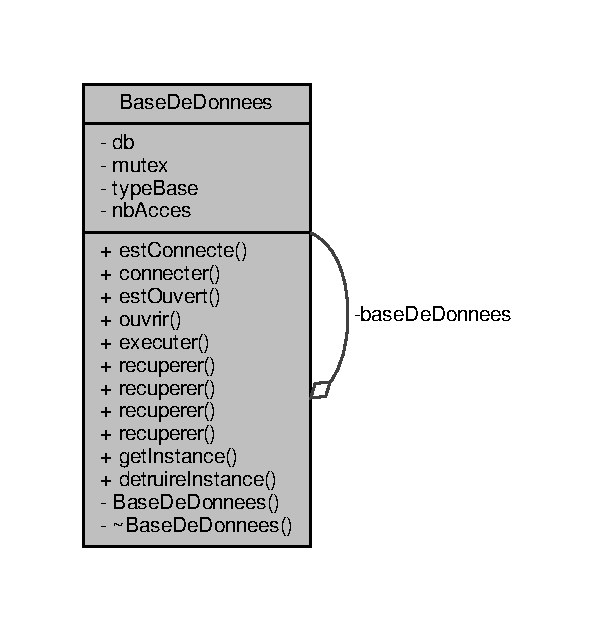
\includegraphics[width=286pt]{class_base_de_donnees__coll__graph}
\end{center}
\end{figure}
\subsubsection*{Fonctions membres publiques}
\begin{DoxyCompactItemize}
\item 
bool \hyperlink{class_base_de_donnees_a00388973f3ec42e5c8e76e7af7e124b2}{est\+Connecte} ()
\item 
bool \hyperlink{class_base_de_donnees_ab2e092285ccc0ee1cce61a1774218561}{connecter} (Q\+String nom\+Base, Q\+String username=\hyperlink{basededonnees_8h_a88b5f5b81fa534553c68802384beff2c}{B\+D\+D\+\_\+\+U\+S\+E\+R\+N\+A\+ME}, Q\+String password=\hyperlink{basededonnees_8h_ae2ded9166ed2553182545e97514c04f7}{B\+D\+D\+\_\+\+P\+A\+S\+S\+W\+O\+RD}, Q\+String serveur=\hyperlink{basededonnees_8h_af06096ec4ec654090fa78ab359d4a0dd}{B\+D\+D\+\_\+\+H\+O\+S\+T\+N\+A\+ME})
\item 
bool \hyperlink{class_base_de_donnees_af9ac332082ffd0dd35e412cefabe5e9c}{est\+Ouvert} ()
\item 
bool \hyperlink{class_base_de_donnees_a7f6a5510b08017b0d99115a84252f186}{ouvrir} (Q\+String fichier\+Base)
\item 
bool \hyperlink{class_base_de_donnees_aa8de5f8f8bb17edc43f5c0ee33712081}{executer} (Q\+String requete)
\item 
bool \hyperlink{class_base_de_donnees_a77539baad389f5acf754cd2cd452403e}{recuperer} (Q\+String requete, Q\+String \&donnees)
\item 
bool \hyperlink{class_base_de_donnees_a2a5c461fa11d404810ae3ebe035d5190}{recuperer} (Q\+String requete, Q\+String\+List \&donnees)
\item 
bool \hyperlink{class_base_de_donnees_af9a76eb2b12df784280c379a4b22af62}{recuperer} (Q\+String requete, Q\+Vector$<$ Q\+String $>$ \&donnees)
\item 
bool \hyperlink{class_base_de_donnees_a68dd0d62ba03b9e8e5aa759d0666cb59}{recuperer} (Q\+String requete, Q\+Vector$<$ Q\+String\+List $>$ \&donnees)
\end{DoxyCompactItemize}
\subsubsection*{Fonctions membres publiques statiques}
\begin{DoxyCompactItemize}
\item 
static \hyperlink{class_base_de_donnees}{Base\+De\+Donnees} $\ast$ \hyperlink{class_base_de_donnees_a80028aa2b6b4fbf30fb2e36357b7d3d3}{get\+Instance} (Q\+String type=\char`\"{}Q\+M\+Y\+S\+QL\char`\"{})
\item 
static void \hyperlink{class_base_de_donnees_a457401c0816b888c77ce915997545f4e}{detruire\+Instance} ()
\end{DoxyCompactItemize}
\subsubsection*{Fonctions membres privées}
\begin{DoxyCompactItemize}
\item 
\hyperlink{class_base_de_donnees_a10dd177f1008f675ab78c2221b2a6750}{Base\+De\+Donnees} (Q\+String type)
\item 
\hyperlink{class_base_de_donnees_a5dc474cdbe003644fb0ca7b8f2ec6b93}{$\sim$\+Base\+De\+Donnees} ()
\end{DoxyCompactItemize}
\subsubsection*{Attributs privés}
\begin{DoxyCompactItemize}
\item 
Q\+Sql\+Database \hyperlink{class_base_de_donnees_a3e738dcf443370c46a541677ab619f06}{db}
\item 
Q\+Mutex \hyperlink{class_base_de_donnees_aa1b4696fac87a740f914aa73739086f2}{mutex}
\end{DoxyCompactItemize}
\subsubsection*{Attributs privés statiques}
\begin{DoxyCompactItemize}
\item 
static \hyperlink{class_base_de_donnees}{Base\+De\+Donnees} $\ast$ \hyperlink{class_base_de_donnees_a822ba0b7cf85b1e48ced8efd3d65e266}{base\+De\+Donnees} = nullptr
\item 
static Q\+String \hyperlink{class_base_de_donnees_ab682b82167f494496a6531bfe522b42b}{type\+Base} = \char`\"{}Q\+M\+Y\+S\+QL\char`\"{}
\item 
static int \hyperlink{class_base_de_donnees_a5099ecb2922bb31d84cd5d4505298a29}{nb\+Acces} = 0
\end{DoxyCompactItemize}


\subsubsection{Description détaillée}
\begin{DoxyAuthor}{Auteur}
Thierry V\+A\+I\+RA
\end{DoxyAuthor}
\begin{DoxyVersion}{Version}
1.\+1 
\end{DoxyVersion}


\subsubsection{Documentation des constructeurs et destructeur}
\mbox{\Hypertarget{class_base_de_donnees_a10dd177f1008f675ab78c2221b2a6750}\label{class_base_de_donnees_a10dd177f1008f675ab78c2221b2a6750}} 
\index{Base\+De\+Donnees@{Base\+De\+Donnees}!Base\+De\+Donnees@{Base\+De\+Donnees}}
\index{Base\+De\+Donnees@{Base\+De\+Donnees}!Base\+De\+Donnees@{Base\+De\+Donnees}}
\paragraph{\texorpdfstring{Base\+De\+Donnees()}{BaseDeDonnees()}}
{\footnotesize\ttfamily Base\+De\+Donnees\+::\+Base\+De\+Donnees (\begin{DoxyParamCaption}\item[{Q\+String}]{type }\end{DoxyParamCaption})\hspace{0.3cm}{\ttfamily [private]}}



Références \hyperlink{class_base_de_donnees_a3e738dcf443370c46a541677ab619f06}{db}, et \hyperlink{class_base_de_donnees_ab682b82167f494496a6531bfe522b42b}{type\+Base}.



Référencé par \hyperlink{class_base_de_donnees_a80028aa2b6b4fbf30fb2e36357b7d3d3}{get\+Instance()}.


\begin{DoxyCode}
00023 \{
00024 \textcolor{preprocessor}{    #ifdef DEBUG\_BASEDEDONNEES}
00025     qDebug() << Q\_FUNC\_INFO << type;
00026 \textcolor{preprocessor}{    #endif}
00027     \hyperlink{class_base_de_donnees_a3e738dcf443370c46a541677ab619f06}{db} = QSqlDatabase::addDatabase(type);
00028     \hyperlink{class_base_de_donnees_ab682b82167f494496a6531bfe522b42b}{typeBase} = type;
00029 \}
\end{DoxyCode}
\mbox{\Hypertarget{class_base_de_donnees_a5dc474cdbe003644fb0ca7b8f2ec6b93}\label{class_base_de_donnees_a5dc474cdbe003644fb0ca7b8f2ec6b93}} 
\index{Base\+De\+Donnees@{Base\+De\+Donnees}!````~Base\+De\+Donnees@{$\sim$\+Base\+De\+Donnees}}
\index{````~Base\+De\+Donnees@{$\sim$\+Base\+De\+Donnees}!Base\+De\+Donnees@{Base\+De\+Donnees}}
\paragraph{\texorpdfstring{$\sim$\+Base\+De\+Donnees()}{~BaseDeDonnees()}}
{\footnotesize\ttfamily Base\+De\+Donnees\+::$\sim$\+Base\+De\+Donnees (\begin{DoxyParamCaption}{ }\end{DoxyParamCaption})\hspace{0.3cm}{\ttfamily [private]}}


\begin{DoxyCode}
00032 \{
00033 \textcolor{preprocessor}{    #ifdef DEBUG\_BASEDEDONNEES}
00034     qDebug() << Q\_FUNC\_INFO;
00035 \textcolor{preprocessor}{    #endif}
00036 \}
\end{DoxyCode}


\subsubsection{Documentation des fonctions membres}
\mbox{\Hypertarget{class_base_de_donnees_ab2e092285ccc0ee1cce61a1774218561}\label{class_base_de_donnees_ab2e092285ccc0ee1cce61a1774218561}} 
\index{Base\+De\+Donnees@{Base\+De\+Donnees}!connecter@{connecter}}
\index{connecter@{connecter}!Base\+De\+Donnees@{Base\+De\+Donnees}}
\paragraph{\texorpdfstring{connecter()}{connecter()}}
{\footnotesize\ttfamily bool Base\+De\+Donnees\+::connecter (\begin{DoxyParamCaption}\item[{Q\+String}]{nom\+Base,  }\item[{Q\+String}]{username = {\ttfamily \hyperlink{basededonnees_8h_a88b5f5b81fa534553c68802384beff2c}{B\+D\+D\+\_\+\+U\+S\+E\+R\+N\+A\+ME}},  }\item[{Q\+String}]{password = {\ttfamily \hyperlink{basededonnees_8h_ae2ded9166ed2553182545e97514c04f7}{B\+D\+D\+\_\+\+P\+A\+S\+S\+W\+O\+RD}},  }\item[{Q\+String}]{serveur = {\ttfamily \hyperlink{basededonnees_8h_af06096ec4ec654090fa78ab359d4a0dd}{B\+D\+D\+\_\+\+H\+O\+S\+T\+N\+A\+ME}} }\end{DoxyParamCaption})}



Références \hyperlink{class_base_de_donnees_a3e738dcf443370c46a541677ab619f06}{db}, \hyperlink{class_base_de_donnees_aa1b4696fac87a740f914aa73739086f2}{mutex}, et \hyperlink{class_base_de_donnees_ab682b82167f494496a6531bfe522b42b}{type\+Base}.


\begin{DoxyCode}
00076 \{
00077     \textcolor{keywordflow}{if}(\hyperlink{class_base_de_donnees_ab682b82167f494496a6531bfe522b42b}{typeBase} != \textcolor{stringliteral}{"QMYSQL"})
00078         \textcolor{keywordflow}{return} \textcolor{keyword}{false};
00079     QMutexLocker verrou(&\hyperlink{class_base_de_donnees_aa1b4696fac87a740f914aa73739086f2}{mutex});
00080     \textcolor{keywordflow}{if}(!\hyperlink{class_base_de_donnees_a3e738dcf443370c46a541677ab619f06}{db}.isOpen())
00081     \{
00082        \hyperlink{class_base_de_donnees_a3e738dcf443370c46a541677ab619f06}{db}.setHostName(serveur);
00083        \hyperlink{class_base_de_donnees_a3e738dcf443370c46a541677ab619f06}{db}.setUserName(username);
00084        \hyperlink{class_base_de_donnees_a3e738dcf443370c46a541677ab619f06}{db}.setPassword(password);
00085        \hyperlink{class_base_de_donnees_a3e738dcf443370c46a541677ab619f06}{db}.setDatabaseName(nomBase);
00086 
00087 \textcolor{preprocessor}{       #ifdef DEBUG\_BASEDEDONNEES}
00088        qDebug() << Q\_FUNC\_INFO;
00089        qDebug() << \textcolor{stringliteral}{"HostName : "} << \hyperlink{class_base_de_donnees_a3e738dcf443370c46a541677ab619f06}{db}.hostName();
00090        qDebug() << \textcolor{stringliteral}{"UserName : "} << \hyperlink{class_base_de_donnees_a3e738dcf443370c46a541677ab619f06}{db}.userName();
00091        qDebug() << \textcolor{stringliteral}{"DatabaseName : "} << \hyperlink{class_base_de_donnees_a3e738dcf443370c46a541677ab619f06}{db}.databaseName();
00092 \textcolor{preprocessor}{       #endif}
00093        \textcolor{keywordflow}{if}(\hyperlink{class_base_de_donnees_a3e738dcf443370c46a541677ab619f06}{db}.open())
00094        \{
00095 \textcolor{preprocessor}{           #ifdef DEBUG\_BASEDEDONNEES}
00096            qDebug() << Q\_FUNC\_INFO << QString::fromUtf8(\textcolor{stringliteral}{"Connexion réussie à %1"}).arg(
      \hyperlink{class_base_de_donnees_a3e738dcf443370c46a541677ab619f06}{db}.hostName());
00097 \textcolor{preprocessor}{           #endif}
00098            \textcolor{keywordflow}{return} \textcolor{keyword}{true};
00099        \}
00100        \textcolor{keywordflow}{else}
00101        \{
00102            qDebug() << Q\_FUNC\_INFO << QString::fromUtf8(\textcolor{stringliteral}{"Erreur : impossible de se connecter à la base de
       données !"});
00103            QMessageBox::critical(\textcolor{keyword}{nullptr}, QString::fromUtf8(\textcolor{stringliteral}{"BaseDeDonnees"}), QString::fromUtf8(\textcolor{stringliteral}{"Impossible
       de se connecter à la base de données !"}));
00104            \textcolor{keywordflow}{return} \textcolor{keyword}{false};
00105        \}
00106     \}
00107     \textcolor{keywordflow}{else}
00108         \textcolor{keywordflow}{return} \textcolor{keyword}{true};
00109 \}
\end{DoxyCode}
\mbox{\Hypertarget{class_base_de_donnees_a457401c0816b888c77ce915997545f4e}\label{class_base_de_donnees_a457401c0816b888c77ce915997545f4e}} 
\index{Base\+De\+Donnees@{Base\+De\+Donnees}!detruire\+Instance@{detruire\+Instance}}
\index{detruire\+Instance@{detruire\+Instance}!Base\+De\+Donnees@{Base\+De\+Donnees}}
\paragraph{\texorpdfstring{detruire\+Instance()}{detruireInstance()}}
{\footnotesize\ttfamily void Base\+De\+Donnees\+::detruire\+Instance (\begin{DoxyParamCaption}{ }\end{DoxyParamCaption})\hspace{0.3cm}{\ttfamily [static]}}



Références \hyperlink{class_base_de_donnees_a822ba0b7cf85b1e48ced8efd3d65e266}{base\+De\+Donnees}, et \hyperlink{class_base_de_donnees_a5099ecb2922bb31d84cd5d4505298a29}{nb\+Acces}.



Référencé par \hyperlink{class_i_h_m_rov_ab861463889934a3b6083b7a29c6adf45}{I\+H\+M\+Rov\+::$\sim$\+I\+H\+M\+Rov()}, et \hyperlink{class_rov_a6e41f712195b9af74fd75b781745d1b5}{Rov\+::$\sim$\+Rov()}.


\begin{DoxyCode}
00051 \{
00052     \textcolor{comment}{// instance ?}
00053     \textcolor{keywordflow}{if}(\hyperlink{class_base_de_donnees_a822ba0b7cf85b1e48ced8efd3d65e266}{baseDeDonnees} != \textcolor{keyword}{nullptr})
00054     \{
00055         \textcolor{keywordflow}{if}(\hyperlink{class_base_de_donnees_a5099ecb2922bb31d84cd5d4505298a29}{nbAcces} > 0)
00056             \hyperlink{class_base_de_donnees_a5099ecb2922bb31d84cd5d4505298a29}{nbAcces}--;
00057 \textcolor{preprocessor}{        #ifdef DEBUG\_BASEDEDONNEES}
00058         qDebug() << Q\_FUNC\_INFO << \textcolor{stringliteral}{"nbAcces restants"} << \hyperlink{class_base_de_donnees_a5099ecb2922bb31d84cd5d4505298a29}{nbAcces};
00059 \textcolor{preprocessor}{        #endif}
00060         \textcolor{comment}{// dernier ?}
00061         \textcolor{keywordflow}{if}(nbAcces == 0)
00062         \{
00063             \textcolor{keyword}{delete} \hyperlink{class_base_de_donnees_a822ba0b7cf85b1e48ced8efd3d65e266}{baseDeDonnees};
00064             \hyperlink{class_base_de_donnees_a822ba0b7cf85b1e48ced8efd3d65e266}{baseDeDonnees} = \textcolor{keyword}{nullptr};
00065         \}
00066     \}
00067 \}
\end{DoxyCode}
\mbox{\Hypertarget{class_base_de_donnees_a00388973f3ec42e5c8e76e7af7e124b2}\label{class_base_de_donnees_a00388973f3ec42e5c8e76e7af7e124b2}} 
\index{Base\+De\+Donnees@{Base\+De\+Donnees}!est\+Connecte@{est\+Connecte}}
\index{est\+Connecte@{est\+Connecte}!Base\+De\+Donnees@{Base\+De\+Donnees}}
\paragraph{\texorpdfstring{est\+Connecte()}{estConnecte()}}
{\footnotesize\ttfamily bool Base\+De\+Donnees\+::est\+Connecte (\begin{DoxyParamCaption}{ }\end{DoxyParamCaption})}



Références \hyperlink{class_base_de_donnees_a3e738dcf443370c46a541677ab619f06}{db}, et \hyperlink{class_base_de_donnees_aa1b4696fac87a740f914aa73739086f2}{mutex}.


\begin{DoxyCode}
00070 \{
00071     QMutexLocker verrou(&\hyperlink{class_base_de_donnees_aa1b4696fac87a740f914aa73739086f2}{mutex});
00072     \textcolor{keywordflow}{return} \hyperlink{class_base_de_donnees_a3e738dcf443370c46a541677ab619f06}{db}.isOpen();
00073 \}
\end{DoxyCode}
\mbox{\Hypertarget{class_base_de_donnees_af9ac332082ffd0dd35e412cefabe5e9c}\label{class_base_de_donnees_af9ac332082ffd0dd35e412cefabe5e9c}} 
\index{Base\+De\+Donnees@{Base\+De\+Donnees}!est\+Ouvert@{est\+Ouvert}}
\index{est\+Ouvert@{est\+Ouvert}!Base\+De\+Donnees@{Base\+De\+Donnees}}
\paragraph{\texorpdfstring{est\+Ouvert()}{estOuvert()}}
{\footnotesize\ttfamily bool Base\+De\+Donnees\+::est\+Ouvert (\begin{DoxyParamCaption}{ }\end{DoxyParamCaption})}



Références \hyperlink{class_base_de_donnees_a3e738dcf443370c46a541677ab619f06}{db}, et \hyperlink{class_base_de_donnees_aa1b4696fac87a740f914aa73739086f2}{mutex}.



Référencé par \hyperlink{class_rov_a5dddd3bd156c134848078296087d090c}{Rov\+::\+Rov()}.


\begin{DoxyCode}
00112 \{
00113     QMutexLocker verrou(&\hyperlink{class_base_de_donnees_aa1b4696fac87a740f914aa73739086f2}{mutex});
00114     \textcolor{keywordflow}{return} \hyperlink{class_base_de_donnees_a3e738dcf443370c46a541677ab619f06}{db}.isOpen();
00115 \}
\end{DoxyCode}
\mbox{\Hypertarget{class_base_de_donnees_aa8de5f8f8bb17edc43f5c0ee33712081}\label{class_base_de_donnees_aa8de5f8f8bb17edc43f5c0ee33712081}} 
\index{Base\+De\+Donnees@{Base\+De\+Donnees}!executer@{executer}}
\index{executer@{executer}!Base\+De\+Donnees@{Base\+De\+Donnees}}
\paragraph{\texorpdfstring{executer()}{executer()}}
{\footnotesize\ttfamily bool Base\+De\+Donnees\+::executer (\begin{DoxyParamCaption}\item[{Q\+String}]{requete }\end{DoxyParamCaption})}



Références \hyperlink{class_base_de_donnees_a3e738dcf443370c46a541677ab619f06}{db}, et \hyperlink{class_base_de_donnees_aa1b4696fac87a740f914aa73739086f2}{mutex}.



Référencé par \hyperlink{class_rov_ae1306036b067e9ad50a09f9dd607a092}{Rov\+::creer\+Nouvelle\+Campagne()}, et \hyperlink{class_rov_adab08abfde381c2915695489b34da6b4}{Rov\+::stocke\+Mesures\+B\+D\+D()}.


\begin{DoxyCode}
00150 \{
00151     QMutexLocker verrou(&\hyperlink{class_base_de_donnees_aa1b4696fac87a740f914aa73739086f2}{mutex});
00152     QSqlQuery r;
00153     \textcolor{keywordtype}{bool} retour;
00154 
00155     \textcolor{keywordflow}{if}(\hyperlink{class_base_de_donnees_a3e738dcf443370c46a541677ab619f06}{db}.isOpen())
00156     \{
00157         \textcolor{keywordflow}{if}(requete.contains(\textcolor{stringliteral}{"UPDATE"}) || requete.contains(\textcolor{stringliteral}{"INSERT"}) || requete.contains(\textcolor{stringliteral}{"DELETE"}))
00158         \{
00159             retour = r.exec(requete);
00160 \textcolor{preprocessor}{            #ifdef DEBUG\_BASEDEDONNEES}
00161             qDebug() << Q\_FUNC\_INFO << QString::fromUtf8(\textcolor{stringliteral}{"Retour %1 pour la requete : %2"}).arg(
      QString::number(retour)).arg(requete);
00162 \textcolor{preprocessor}{            #endif}
00163             \textcolor{keywordflow}{if}(retour)
00164             \{
00165                 \textcolor{keywordflow}{return} \textcolor{keyword}{true};
00166             \}
00167             \textcolor{keywordflow}{else}
00168             \{
00169                 qDebug() << Q\_FUNC\_INFO << QString::fromUtf8(\textcolor{stringliteral}{"Erreur : %1 pour la requête %2"}).arg(r.
      lastError().text()).arg(requete);
00170                 \textcolor{keywordflow}{return} \textcolor{keyword}{false};
00171             \}
00172         \}
00173         \textcolor{keywordflow}{else}
00174         \{
00175             qDebug() << Q\_FUNC\_INFO << QString::fromUtf8(\textcolor{stringliteral}{"Erreur : requête %1 non autorisée !"}).arg(requete
      );
00176             \textcolor{keywordflow}{return} \textcolor{keyword}{false};
00177         \}
00178     \}
00179     \textcolor{keywordflow}{else}
00180         \textcolor{keywordflow}{return} \textcolor{keyword}{false};
00181 
00182 \}
\end{DoxyCode}
\mbox{\Hypertarget{class_base_de_donnees_a80028aa2b6b4fbf30fb2e36357b7d3d3}\label{class_base_de_donnees_a80028aa2b6b4fbf30fb2e36357b7d3d3}} 
\index{Base\+De\+Donnees@{Base\+De\+Donnees}!get\+Instance@{get\+Instance}}
\index{get\+Instance@{get\+Instance}!Base\+De\+Donnees@{Base\+De\+Donnees}}
\paragraph{\texorpdfstring{get\+Instance()}{getInstance()}}
{\footnotesize\ttfamily \hyperlink{class_base_de_donnees}{Base\+De\+Donnees} $\ast$ Base\+De\+Donnees\+::get\+Instance (\begin{DoxyParamCaption}\item[{Q\+String}]{type = {\ttfamily \char`\"{}QMYSQL\char`\"{}} }\end{DoxyParamCaption})\hspace{0.3cm}{\ttfamily [static]}}



Références \hyperlink{class_base_de_donnees_a10dd177f1008f675ab78c2221b2a6750}{Base\+De\+Donnees()}, \hyperlink{class_base_de_donnees_a822ba0b7cf85b1e48ced8efd3d65e266}{base\+De\+Donnees}, et \hyperlink{class_base_de_donnees_a5099ecb2922bb31d84cd5d4505298a29}{nb\+Acces}.



Référencé par \hyperlink{class_rov_a5dddd3bd156c134848078296087d090c}{Rov\+::\+Rov()}.


\begin{DoxyCode}
00039 \{
00040     \textcolor{keywordflow}{if}(\hyperlink{class_base_de_donnees_a822ba0b7cf85b1e48ced8efd3d65e266}{baseDeDonnees} == \textcolor{keyword}{nullptr})
00041         \hyperlink{class_base_de_donnees_a822ba0b7cf85b1e48ced8efd3d65e266}{baseDeDonnees} = \textcolor{keyword}{new} \hyperlink{class_base_de_donnees_a10dd177f1008f675ab78c2221b2a6750}{BaseDeDonnees}(type);
00042     \hyperlink{class_base_de_donnees_a5099ecb2922bb31d84cd5d4505298a29}{nbAcces}++;
00043 \textcolor{preprocessor}{    #ifdef DEBUG\_BASEDEDONNEES}
00044     qDebug() << Q\_FUNC\_INFO << \textcolor{stringliteral}{"nbAcces"} << \hyperlink{class_base_de_donnees_a5099ecb2922bb31d84cd5d4505298a29}{nbAcces};
00045 \textcolor{preprocessor}{    #endif}
00046 
00047     \textcolor{keywordflow}{return} \hyperlink{class_base_de_donnees_a822ba0b7cf85b1e48ced8efd3d65e266}{baseDeDonnees};
00048 \}
\end{DoxyCode}
\mbox{\Hypertarget{class_base_de_donnees_a7f6a5510b08017b0d99115a84252f186}\label{class_base_de_donnees_a7f6a5510b08017b0d99115a84252f186}} 
\index{Base\+De\+Donnees@{Base\+De\+Donnees}!ouvrir@{ouvrir}}
\index{ouvrir@{ouvrir}!Base\+De\+Donnees@{Base\+De\+Donnees}}
\paragraph{\texorpdfstring{ouvrir()}{ouvrir()}}
{\footnotesize\ttfamily bool Base\+De\+Donnees\+::ouvrir (\begin{DoxyParamCaption}\item[{Q\+String}]{fichier\+Base }\end{DoxyParamCaption})}



Références \hyperlink{class_base_de_donnees_a3e738dcf443370c46a541677ab619f06}{db}, \hyperlink{class_base_de_donnees_aa1b4696fac87a740f914aa73739086f2}{mutex}, et \hyperlink{class_base_de_donnees_ab682b82167f494496a6531bfe522b42b}{type\+Base}.



Référencé par \hyperlink{class_rov_a5dddd3bd156c134848078296087d090c}{Rov\+::\+Rov()}.


\begin{DoxyCode}
00118 \{
00119     \textcolor{keywordflow}{if}(\hyperlink{class_base_de_donnees_ab682b82167f494496a6531bfe522b42b}{typeBase} != \textcolor{stringliteral}{"QSQLITE"})
00120         \textcolor{keywordflow}{return} \textcolor{keyword}{false};
00121     QMutexLocker verrou(&\hyperlink{class_base_de_donnees_aa1b4696fac87a740f914aa73739086f2}{mutex});
00122     \textcolor{keywordflow}{if}(!\hyperlink{class_base_de_donnees_a3e738dcf443370c46a541677ab619f06}{db}.isOpen())
00123     \{
00124        \hyperlink{class_base_de_donnees_a3e738dcf443370c46a541677ab619f06}{db}.setDatabaseName(fichierBase);
00125 
00126 \textcolor{preprocessor}{       #ifdef DEBUG\_BASEDEDONNEES}
00127        qDebug() << Q\_FUNC\_INFO << \hyperlink{class_base_de_donnees_a3e738dcf443370c46a541677ab619f06}{db}.databaseName();       
00128 \textcolor{preprocessor}{       #endif}
00129        \textcolor{keywordflow}{if}(\hyperlink{class_base_de_donnees_a3e738dcf443370c46a541677ab619f06}{db}.open())
00130        \{
00131 \textcolor{preprocessor}{           #ifdef DEBUG\_BASEDEDONNEES}
00132            qDebug() << Q\_FUNC\_INFO << QString::fromUtf8(\textcolor{stringliteral}{"Ouvertir réussie à %1"}).arg(
      \hyperlink{class_base_de_donnees_a3e738dcf443370c46a541677ab619f06}{db}.databaseName());
00133 \textcolor{preprocessor}{           #endif}
00134 
00135            \textcolor{keywordflow}{return} \textcolor{keyword}{true};
00136        \}
00137        \textcolor{keywordflow}{else}
00138        \{
00139            qDebug() << Q\_FUNC\_INFO << QString::fromUtf8(\textcolor{stringliteral}{"Erreur : impossible d'ouvrir la base de données !"}
      );
00140            QMessageBox::critical(\textcolor{keyword}{nullptr}, QString::fromUtf8(\textcolor{stringliteral}{"BaseDeDonnees"}), QString::fromUtf8(\textcolor{stringliteral}{"Impossible
       d'ouvrir la base de données !"}));
00141            \textcolor{keywordflow}{return} \textcolor{keyword}{false};
00142        \}
00143     \}
00144     \textcolor{keywordflow}{else}
00145         \textcolor{keywordflow}{return} \textcolor{keyword}{true};
00146 \}
\end{DoxyCode}
\mbox{\Hypertarget{class_base_de_donnees_a77539baad389f5acf754cd2cd452403e}\label{class_base_de_donnees_a77539baad389f5acf754cd2cd452403e}} 
\index{Base\+De\+Donnees@{Base\+De\+Donnees}!recuperer@{recuperer}}
\index{recuperer@{recuperer}!Base\+De\+Donnees@{Base\+De\+Donnees}}
\paragraph{\texorpdfstring{recuperer()}{recuperer()}\hspace{0.1cm}{\footnotesize\ttfamily [1/4]}}
{\footnotesize\ttfamily bool Base\+De\+Donnees\+::recuperer (\begin{DoxyParamCaption}\item[{Q\+String}]{requete,  }\item[{Q\+String \&}]{donnees }\end{DoxyParamCaption})}



Références \hyperlink{class_base_de_donnees_a3e738dcf443370c46a541677ab619f06}{db}, et \hyperlink{class_base_de_donnees_aa1b4696fac87a740f914aa73739086f2}{mutex}.



Référencé par \hyperlink{class_rov_ae1306036b067e9ad50a09f9dd607a092}{Rov\+::creer\+Nouvelle\+Campagne()}, \hyperlink{class_rov_a490eefb90bf28e83f181d770f0f52446}{Rov\+::recuperer\+Liste\+Noms\+Operateurs()}, et \hyperlink{class_rov_a84dece742f5c4c903ada4f25c869597f}{Rov\+::recuperer\+Liste\+Prenoms\+Operateurs()}.


\begin{DoxyCode}
00188 \{
00189     QMutexLocker verrou(&\hyperlink{class_base_de_donnees_aa1b4696fac87a740f914aa73739086f2}{mutex});
00190     QSqlQuery r;
00191     \textcolor{keywordtype}{bool} retour;
00192 
00193     \textcolor{keywordflow}{if}(\hyperlink{class_base_de_donnees_a3e738dcf443370c46a541677ab619f06}{db}.isOpen())
00194     \{
00195         \textcolor{keywordflow}{if}(requete.contains(\textcolor{stringliteral}{"SELECT"}))
00196         \{
00197             retour = r.exec(requete);
00198 \textcolor{preprocessor}{            #ifdef DEBUG\_BASEDEDONNEES}
00199             qDebug() << Q\_FUNC\_INFO << QString::fromUtf8(\textcolor{stringliteral}{"Retour %1 pour la requete : %2"}).arg(
      QString::number(retour)).arg(requete);
00200 \textcolor{preprocessor}{            #endif}
00201             \textcolor{keywordflow}{if}(retour)
00202             \{
00203                 \textcolor{comment}{// on se positionne sur l'enregistrement}
00204                 r.first();
00205 
00206                 \textcolor{comment}{// on vérifie l'état de l'enregistrement retourné}
00207                 \textcolor{keywordflow}{if}(!r.isValid())
00208                 \{
00209 \textcolor{preprocessor}{                    #ifdef DEBUG\_BASEDEDONNEES}
00210                     qDebug() << Q\_FUNC\_INFO << QString::fromUtf8(\textcolor{stringliteral}{"Résultat non valide !"});
00211 \textcolor{preprocessor}{                    #endif}
00212                     \textcolor{keywordflow}{return} \textcolor{keyword}{false};
00213                 \}
00214 
00215                 \textcolor{comment}{// on récupère sous forme de QString la valeur du champ}
00216                 \textcolor{keywordflow}{if}(r.isNull(0))
00217                 \{
00218 \textcolor{preprocessor}{                    #ifdef DEBUG\_BASEDEDONNEES}
00219                     qDebug() << Q\_FUNC\_INFO << QString::fromUtf8(\textcolor{stringliteral}{"Aucun résultat !"});
00220 \textcolor{preprocessor}{                    #endif}
00221                     \textcolor{keywordflow}{return} \textcolor{keyword}{false};
00222                 \}
00223                 donnees = r.value(0).toString();
00224 \textcolor{preprocessor}{                #ifdef DEBUG\_BASEDEDONNEES}
00225                 qDebug() << Q\_FUNC\_INFO << \textcolor{stringliteral}{"Enregistrement -> "} << donnees;
00226 \textcolor{preprocessor}{                #endif}
00227                 \textcolor{keywordflow}{return} \textcolor{keyword}{true};
00228             \}
00229             \textcolor{keywordflow}{else}
00230             \{
00231                 qDebug() << Q\_FUNC\_INFO << QString::fromUtf8(\textcolor{stringliteral}{"Erreur : %1 pour la requête %2"}).arg(r.
      lastError().text()).arg(requete);
00232                 \textcolor{keywordflow}{return} \textcolor{keyword}{false};
00233             \}
00234         \}
00235         \textcolor{keywordflow}{else}
00236         \{
00237             qDebug() << Q\_FUNC\_INFO << QString::fromUtf8(\textcolor{stringliteral}{"Erreur : requête %1 non autorisée !"}).arg(requete
      );
00238             \textcolor{keywordflow}{return} \textcolor{keyword}{false};
00239         \}
00240     \}
00241     \textcolor{keywordflow}{else}
00242         \textcolor{keywordflow}{return} \textcolor{keyword}{false};
00243 \}
\end{DoxyCode}
\mbox{\Hypertarget{class_base_de_donnees_a2a5c461fa11d404810ae3ebe035d5190}\label{class_base_de_donnees_a2a5c461fa11d404810ae3ebe035d5190}} 
\index{Base\+De\+Donnees@{Base\+De\+Donnees}!recuperer@{recuperer}}
\index{recuperer@{recuperer}!Base\+De\+Donnees@{Base\+De\+Donnees}}
\paragraph{\texorpdfstring{recuperer()}{recuperer()}\hspace{0.1cm}{\footnotesize\ttfamily [2/4]}}
{\footnotesize\ttfamily bool Base\+De\+Donnees\+::recuperer (\begin{DoxyParamCaption}\item[{Q\+String}]{requete,  }\item[{Q\+String\+List \&}]{donnees }\end{DoxyParamCaption})}



Références \hyperlink{class_base_de_donnees_a3e738dcf443370c46a541677ab619f06}{db}, et \hyperlink{class_base_de_donnees_aa1b4696fac87a740f914aa73739086f2}{mutex}.


\begin{DoxyCode}
00249 \{
00250     QMutexLocker verrou(&\hyperlink{class_base_de_donnees_aa1b4696fac87a740f914aa73739086f2}{mutex});
00251     QSqlQuery r;
00252     \textcolor{keywordtype}{bool} retour;
00253 
00254     \textcolor{keywordflow}{if}(\hyperlink{class_base_de_donnees_a3e738dcf443370c46a541677ab619f06}{db}.isOpen())
00255     \{
00256         \textcolor{keywordflow}{if}(requete.contains(\textcolor{stringliteral}{"SELECT"}))
00257         \{
00258             retour = r.exec(requete);
00259 \textcolor{preprocessor}{            #ifdef DEBUG\_BASEDEDONNEES}
00260             qDebug() << QString::fromUtf8(\textcolor{stringliteral}{"<BaseDeDonnees::recuperer(QString, QStringList)> retour %1 pour
       la requete : %2"}).arg(QString::number(retour)).arg(requete);
00261 \textcolor{preprocessor}{            #endif}
00262             \textcolor{keywordflow}{if}(retour)
00263             \{
00264                 \textcolor{comment}{// on se positionne sur l'enregistrement}
00265                 r.first();
00266 
00267                 \textcolor{comment}{// on vérifie l'état de l'enregistrement retourné}
00268                 \textcolor{keywordflow}{if}(!r.isValid())
00269                 \{
00270 \textcolor{preprocessor}{                    #ifdef DEBUG\_BASEDEDONNEES}
00271                     qDebug() << Q\_FUNC\_INFO << QString::fromUtf8(\textcolor{stringliteral}{"Résultat non valide !"});
00272 \textcolor{preprocessor}{                    #endif}
00273                     \textcolor{keywordflow}{return} \textcolor{keyword}{false};
00274                 \}
00275 
00276                 \textcolor{comment}{// on récupère sous forme de QString la valeur de tous les champs sélectionnés}
00277                 \textcolor{comment}{// et on les stocke dans une liste de QString}
00278                 \textcolor{keywordflow}{for}(\textcolor{keywordtype}{int} i=0;i<r.record().count();i++)
00279                     \textcolor{keywordflow}{if}(!r.isNull(i))
00280                         donnees << r.value(i).toString();
00281 \textcolor{preprocessor}{                #ifdef DEBUG\_BASEDEDONNEES}
00282                 qDebug() << Q\_FUNC\_INFO << \textcolor{stringliteral}{"Enregistrement -> "} << donnees;
00283 \textcolor{preprocessor}{                #endif}
00284                 \textcolor{keywordflow}{return} \textcolor{keyword}{true};
00285             \}
00286             \textcolor{keywordflow}{else}
00287             \{
00288                 qDebug() << Q\_FUNC\_INFO << QString::fromUtf8(\textcolor{stringliteral}{"Erreur : %1 pour la requête %2"}).arg(r.
      lastError().text()).arg(requete);
00289                 \textcolor{keywordflow}{return} \textcolor{keyword}{false};
00290             \}
00291         \}
00292         \textcolor{keywordflow}{else}
00293         \{
00294             qDebug() << Q\_FUNC\_INFO << QString::fromUtf8(\textcolor{stringliteral}{"Erreur : requête %1 non autorisée !"}).arg(requete
      );
00295             \textcolor{keywordflow}{return} \textcolor{keyword}{false};
00296         \}
00297     \}
00298     \textcolor{keywordflow}{else}
00299         \textcolor{keywordflow}{return} \textcolor{keyword}{false};
00300 \}
\end{DoxyCode}
\mbox{\Hypertarget{class_base_de_donnees_af9a76eb2b12df784280c379a4b22af62}\label{class_base_de_donnees_af9a76eb2b12df784280c379a4b22af62}} 
\index{Base\+De\+Donnees@{Base\+De\+Donnees}!recuperer@{recuperer}}
\index{recuperer@{recuperer}!Base\+De\+Donnees@{Base\+De\+Donnees}}
\paragraph{\texorpdfstring{recuperer()}{recuperer()}\hspace{0.1cm}{\footnotesize\ttfamily [3/4]}}
{\footnotesize\ttfamily bool Base\+De\+Donnees\+::recuperer (\begin{DoxyParamCaption}\item[{Q\+String}]{requete,  }\item[{Q\+Vector$<$ Q\+String $>$ \&}]{donnees }\end{DoxyParamCaption})}



Références \hyperlink{class_base_de_donnees_a3e738dcf443370c46a541677ab619f06}{db}, et \hyperlink{class_base_de_donnees_aa1b4696fac87a740f914aa73739086f2}{mutex}.


\begin{DoxyCode}
00306 \{
00307     QMutexLocker verrou(&\hyperlink{class_base_de_donnees_aa1b4696fac87a740f914aa73739086f2}{mutex});
00308     QSqlQuery r;
00309     \textcolor{keywordtype}{bool} retour;
00310     QString data;
00311 
00312     \textcolor{keywordflow}{if}(\hyperlink{class_base_de_donnees_a3e738dcf443370c46a541677ab619f06}{db}.isOpen())
00313     \{
00314         \textcolor{keywordflow}{if}(requete.contains(\textcolor{stringliteral}{"SELECT"}))
00315         \{
00316             retour = r.exec(requete);
00317 \textcolor{preprocessor}{            #ifdef DEBUG\_BASEDEDONNEES}
00318             qDebug() << Q\_FUNC\_INFO << QString::fromUtf8(\textcolor{stringliteral}{"Retour %1 pour la requete : %2"}).arg(
      QString::number(retour)).arg(requete);
00319 \textcolor{preprocessor}{            #endif}
00320             \textcolor{keywordflow}{if}(retour)
00321             \{
00322                 \textcolor{comment}{// pour chaque enregistrement}
00323                 \textcolor{keywordflow}{while} ( r.next() )
00324                 \{
00325                     \textcolor{comment}{// on récupère sous forme de QString la valeur du champs sélectionné}
00326                     data = r.value(0).toString();
00327 
00328 \textcolor{preprocessor}{                    #ifdef DEBUG\_BASEDEDONNEES}
00329                     \textcolor{comment}{//qDebug() << Q\_FUNC\_INFO << "Enregistrement -> " << data;}
00330 \textcolor{preprocessor}{                    #endif}
00331 
00332                     \textcolor{comment}{// on stocke l'enregistrement dans le QVector}
00333                     donnees.push\_back(data);
00334                 \}
00335 \textcolor{preprocessor}{                #ifdef DEBUG\_BASEDEDONNEES}
00336                 qDebug() << Q\_FUNC\_INFO << \textcolor{stringliteral}{"Enregistrement -> "} << donnees;
00337 \textcolor{preprocessor}{                #endif}
00338                 \textcolor{keywordflow}{return} \textcolor{keyword}{true};
00339             \}
00340             \textcolor{keywordflow}{else}
00341             \{
00342                 qDebug() << Q\_FUNC\_INFO << QString::fromUtf8(\textcolor{stringliteral}{"Erreur : %1 pour la requête %2"}).arg(r.
      lastError().text()).arg(requete);
00343                 \textcolor{keywordflow}{return} \textcolor{keyword}{false};
00344             \}
00345         \}
00346         \textcolor{keywordflow}{else}
00347         \{
00348             qDebug() << Q\_FUNC\_INFO << QString::fromUtf8(\textcolor{stringliteral}{"Erreur : requête %1 non autorisée !"}).arg(requete
      );
00349             \textcolor{keywordflow}{return} \textcolor{keyword}{false};
00350         \}
00351     \}
00352     \textcolor{keywordflow}{else}
00353         \textcolor{keywordflow}{return} \textcolor{keyword}{false};
00354 \}
\end{DoxyCode}
\mbox{\Hypertarget{class_base_de_donnees_a68dd0d62ba03b9e8e5aa759d0666cb59}\label{class_base_de_donnees_a68dd0d62ba03b9e8e5aa759d0666cb59}} 
\index{Base\+De\+Donnees@{Base\+De\+Donnees}!recuperer@{recuperer}}
\index{recuperer@{recuperer}!Base\+De\+Donnees@{Base\+De\+Donnees}}
\paragraph{\texorpdfstring{recuperer()}{recuperer()}\hspace{0.1cm}{\footnotesize\ttfamily [4/4]}}
{\footnotesize\ttfamily bool Base\+De\+Donnees\+::recuperer (\begin{DoxyParamCaption}\item[{Q\+String}]{requete,  }\item[{Q\+Vector$<$ Q\+String\+List $>$ \&}]{donnees }\end{DoxyParamCaption})}



Références \hyperlink{class_base_de_donnees_a3e738dcf443370c46a541677ab619f06}{db}, et \hyperlink{class_base_de_donnees_aa1b4696fac87a740f914aa73739086f2}{mutex}.


\begin{DoxyCode}
00360 \{
00361     QMutexLocker verrou(&\hyperlink{class_base_de_donnees_aa1b4696fac87a740f914aa73739086f2}{mutex});
00362     QSqlQuery r;
00363     \textcolor{keywordtype}{bool} retour;
00364     QStringList data;
00365 
00366     \textcolor{keywordflow}{if}(\hyperlink{class_base_de_donnees_a3e738dcf443370c46a541677ab619f06}{db}.isOpen())
00367     \{
00368         \textcolor{keywordflow}{if}(requete.contains(\textcolor{stringliteral}{"SELECT"}))
00369         \{
00370             retour = r.exec(requete);
00371 \textcolor{preprocessor}{            #ifdef DEBUG\_BASEDEDONNEES}
00372             qDebug() << Q\_FUNC\_INFO << QString::fromUtf8(\textcolor{stringliteral}{"Retour %1 pour la requete : %2"}).arg(
      QString::number(retour)).arg(requete);
00373 \textcolor{preprocessor}{            #endif}
00374             \textcolor{keywordflow}{if}(retour)
00375             \{
00376                 \textcolor{comment}{// pour chaque enregistrement}
00377                 \textcolor{keywordflow}{while} ( r.next() )
00378                 \{
00379                     \textcolor{comment}{// on récupère sous forme de QString la valeur de tous les champs sélectionnés}
00380                     \textcolor{comment}{// et on les stocke dans une liste de QString}
00381                     \textcolor{keywordflow}{for}(\textcolor{keywordtype}{int} i=0;i<r.record().count();i++)
00382                         data << r.value(i).toString();
00383 
00384 \textcolor{preprocessor}{                    #ifdef DEBUG\_BASEDEDONNEES}
00385                     \textcolor{comment}{//qDebug() << Q\_FUNC\_INFO << "Enregistrement -> " << data;}
00386                     \textcolor{comment}{/*for(int i=0;i<r.record().count();i++)}
00387 \textcolor{comment}{                        qDebug() << r.value(i).toString();*/}
00388 \textcolor{preprocessor}{                    #endif}
00389 
00390                     \textcolor{comment}{// on stocke l'enregistrement dans le QVector}
00391                     donnees.push\_back(data);
00392 
00393                     \textcolor{comment}{// on efface la liste de QString pour le prochain enregistrement}
00394                     data.clear();
00395                 \}
00396 \textcolor{preprocessor}{                #ifdef DEBUG\_BASEDEDONNEES}
00397                 qDebug() << Q\_FUNC\_INFO << \textcolor{stringliteral}{"Enregistrement -> "} << donnees;
00398 \textcolor{preprocessor}{                #endif}
00399                 \textcolor{keywordflow}{return} \textcolor{keyword}{true};
00400             \}
00401             \textcolor{keywordflow}{else}
00402             \{
00403                 qDebug() << Q\_FUNC\_INFO << QString::fromUtf8(\textcolor{stringliteral}{"Erreur : %1 pour la requête %2"}).arg(r.
      lastError().text()).arg(requete);
00404                 \textcolor{keywordflow}{return} \textcolor{keyword}{false};
00405             \}
00406         \}
00407         \textcolor{keywordflow}{else}
00408         \{
00409             qDebug() << Q\_FUNC\_INFO << QString::fromUtf8(\textcolor{stringliteral}{"Erreur : requête %1 non autorisée !"}).arg(requete
      );
00410             \textcolor{keywordflow}{return} \textcolor{keyword}{false};
00411         \}
00412     \}
00413     \textcolor{keywordflow}{else}
00414         \textcolor{keywordflow}{return} \textcolor{keyword}{false};
00415 \}
\end{DoxyCode}


\subsubsection{Documentation des données membres}
\mbox{\Hypertarget{class_base_de_donnees_a822ba0b7cf85b1e48ced8efd3d65e266}\label{class_base_de_donnees_a822ba0b7cf85b1e48ced8efd3d65e266}} 
\index{Base\+De\+Donnees@{Base\+De\+Donnees}!base\+De\+Donnees@{base\+De\+Donnees}}
\index{base\+De\+Donnees@{base\+De\+Donnees}!Base\+De\+Donnees@{Base\+De\+Donnees}}
\paragraph{\texorpdfstring{base\+De\+Donnees}{baseDeDonnees}}
{\footnotesize\ttfamily \hyperlink{class_base_de_donnees}{Base\+De\+Donnees} $\ast$ Base\+De\+Donnees\+::base\+De\+Donnees = nullptr\hspace{0.3cm}{\ttfamily [static]}, {\ttfamily [private]}}



Référencé par \hyperlink{class_base_de_donnees_a457401c0816b888c77ce915997545f4e}{detruire\+Instance()}, et \hyperlink{class_base_de_donnees_a80028aa2b6b4fbf30fb2e36357b7d3d3}{get\+Instance()}.

\mbox{\Hypertarget{class_base_de_donnees_a3e738dcf443370c46a541677ab619f06}\label{class_base_de_donnees_a3e738dcf443370c46a541677ab619f06}} 
\index{Base\+De\+Donnees@{Base\+De\+Donnees}!db@{db}}
\index{db@{db}!Base\+De\+Donnees@{Base\+De\+Donnees}}
\paragraph{\texorpdfstring{db}{db}}
{\footnotesize\ttfamily Q\+Sql\+Database Base\+De\+Donnees\+::db\hspace{0.3cm}{\ttfamily [private]}}



Référencé par \hyperlink{class_base_de_donnees_a10dd177f1008f675ab78c2221b2a6750}{Base\+De\+Donnees()}, \hyperlink{class_base_de_donnees_ab2e092285ccc0ee1cce61a1774218561}{connecter()}, \hyperlink{class_base_de_donnees_a00388973f3ec42e5c8e76e7af7e124b2}{est\+Connecte()}, \hyperlink{class_base_de_donnees_af9ac332082ffd0dd35e412cefabe5e9c}{est\+Ouvert()}, \hyperlink{class_base_de_donnees_aa8de5f8f8bb17edc43f5c0ee33712081}{executer()}, \hyperlink{class_base_de_donnees_a7f6a5510b08017b0d99115a84252f186}{ouvrir()}, et \hyperlink{class_base_de_donnees_a77539baad389f5acf754cd2cd452403e}{recuperer()}.

\mbox{\Hypertarget{class_base_de_donnees_aa1b4696fac87a740f914aa73739086f2}\label{class_base_de_donnees_aa1b4696fac87a740f914aa73739086f2}} 
\index{Base\+De\+Donnees@{Base\+De\+Donnees}!mutex@{mutex}}
\index{mutex@{mutex}!Base\+De\+Donnees@{Base\+De\+Donnees}}
\paragraph{\texorpdfstring{mutex}{mutex}}
{\footnotesize\ttfamily Q\+Mutex Base\+De\+Donnees\+::mutex\hspace{0.3cm}{\ttfamily [private]}}



Référencé par \hyperlink{class_base_de_donnees_ab2e092285ccc0ee1cce61a1774218561}{connecter()}, \hyperlink{class_base_de_donnees_a00388973f3ec42e5c8e76e7af7e124b2}{est\+Connecte()}, \hyperlink{class_base_de_donnees_af9ac332082ffd0dd35e412cefabe5e9c}{est\+Ouvert()}, \hyperlink{class_base_de_donnees_aa8de5f8f8bb17edc43f5c0ee33712081}{executer()}, \hyperlink{class_base_de_donnees_a7f6a5510b08017b0d99115a84252f186}{ouvrir()}, et \hyperlink{class_base_de_donnees_a77539baad389f5acf754cd2cd452403e}{recuperer()}.

\mbox{\Hypertarget{class_base_de_donnees_a5099ecb2922bb31d84cd5d4505298a29}\label{class_base_de_donnees_a5099ecb2922bb31d84cd5d4505298a29}} 
\index{Base\+De\+Donnees@{Base\+De\+Donnees}!nb\+Acces@{nb\+Acces}}
\index{nb\+Acces@{nb\+Acces}!Base\+De\+Donnees@{Base\+De\+Donnees}}
\paragraph{\texorpdfstring{nb\+Acces}{nbAcces}}
{\footnotesize\ttfamily int Base\+De\+Donnees\+::nb\+Acces = 0\hspace{0.3cm}{\ttfamily [static]}, {\ttfamily [private]}}



Référencé par \hyperlink{class_base_de_donnees_a457401c0816b888c77ce915997545f4e}{detruire\+Instance()}, et \hyperlink{class_base_de_donnees_a80028aa2b6b4fbf30fb2e36357b7d3d3}{get\+Instance()}.

\mbox{\Hypertarget{class_base_de_donnees_ab682b82167f494496a6531bfe522b42b}\label{class_base_de_donnees_ab682b82167f494496a6531bfe522b42b}} 
\index{Base\+De\+Donnees@{Base\+De\+Donnees}!type\+Base@{type\+Base}}
\index{type\+Base@{type\+Base}!Base\+De\+Donnees@{Base\+De\+Donnees}}
\paragraph{\texorpdfstring{type\+Base}{typeBase}}
{\footnotesize\ttfamily Q\+String Base\+De\+Donnees\+::type\+Base = \char`\"{}Q\+M\+Y\+S\+QL\char`\"{}\hspace{0.3cm}{\ttfamily [static]}, {\ttfamily [private]}}



Référencé par \hyperlink{class_base_de_donnees_a10dd177f1008f675ab78c2221b2a6750}{Base\+De\+Donnees()}, \hyperlink{class_base_de_donnees_ab2e092285ccc0ee1cce61a1774218561}{connecter()}, et \hyperlink{class_base_de_donnees_a7f6a5510b08017b0d99115a84252f186}{ouvrir()}.



La documentation de cette classe a été générée à partir des fichiers suivants \+:\begin{DoxyCompactItemize}
\item 
\hyperlink{basededonnees_8h}{basededonnees.\+h}\item 
\hyperlink{basededonnees_8cpp}{basededonnees.\+cpp}\end{DoxyCompactItemize}

\hypertarget{class_bras}{}\subsection{Référence de la classe Bras}
\label{class_bras}\index{Bras@{Bras}}


Déclaration de la classe \hyperlink{class_bras}{Bras}. Réceptionne les signaux de la manette destiné aux mouvements du bras, et émet les trames correspondantes.  




{\ttfamily \#include $<$bras.\+h$>$}



Graphe de collaboration de Bras\+:
\nopagebreak
\begin{figure}[H]
\begin{center}
\leavevmode
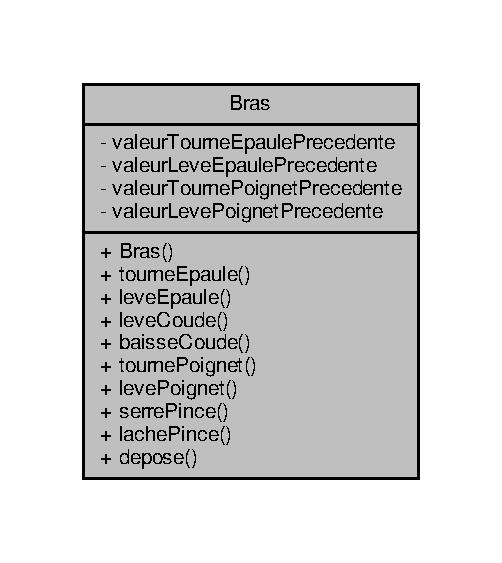
\includegraphics[width=241pt]{class_bras__coll__graph}
\end{center}
\end{figure}
\subsubsection*{Connecteurs publics}
\begin{DoxyCompactItemize}
\item 
void \hyperlink{class_bras_aaeacb18f22532a63559fc8430118169e}{tourne\+Epaule} (double valeur)
\begin{DoxyCompactList}\small\item\em Contrôle la rotation de l\textquotesingle{}épaule (entre autre, la direction du bras), en émettant la trame correspondante. Correspond au joystick droite de la manette. \end{DoxyCompactList}\item 
void \hyperlink{class_bras_ac8f658db87d03bfbba6faa535326cc3a}{leve\+Epaule} (double valeur)
\begin{DoxyCompactList}\small\item\em Contrôle l\textquotesingle{}angle de levé de l\textquotesingle{}épaule, en émettant la trame correspondante. Correspond au joystick droite de la manette. \end{DoxyCompactList}\item 
void \hyperlink{class_bras_a197686a4ff55b4fe2384b2af44b8228b}{leve\+Coude} (bool appuye)
\begin{DoxyCompactList}\small\item\em Permet de lever le coude, en émettant la trame correspondante. Correspond au bouton triangle de la manette. \end{DoxyCompactList}\item 
void \hyperlink{class_bras_a4b8e4791a454fcf884b1e7217a16a326}{baisse\+Coude} (bool appuye)
\begin{DoxyCompactList}\small\item\em Permet de plier le coude, en émettant la trame correspondante. Correspond au bouton X de la manette. \end{DoxyCompactList}\item 
void \hyperlink{class_bras_a15beae8aa104c2e689614486646ab402}{tourne\+Poignet} (double valeur)
\begin{DoxyCompactList}\small\item\em Permet de pivoter le poignet, en émettant la trame correspondante. Correspond au joystick gauche axe X de la manette. \end{DoxyCompactList}\item 
void \hyperlink{class_bras_ac95f54d8b02e7c88081f482fbbc40aef}{leve\+Poignet} (double valeur)
\begin{DoxyCompactList}\small\item\em Permet de lever ou baisser le poignet, en émettant la trame correspondante. Correspond au joystick gauche axe Y de la manette. \end{DoxyCompactList}\item 
void \hyperlink{class_bras_a55e143cf8e696ed214809ae25fb558d5}{serre\+Pince} (bool appuye)
\begin{DoxyCompactList}\small\item\em Permet de serrer la pince, en émettant la trame correspondante. Correspond au bouton R1 de la manette. \end{DoxyCompactList}\item 
void \hyperlink{class_bras_a246e835f25bd61f0618c58aafea99ea1}{lache\+Pince} (bool appuye)
\begin{DoxyCompactList}\small\item\em Permet de relâcher la pince, en émettant la trame correspondante. Correspond au bouton L1 de la manette. \end{DoxyCompactList}\item 
void \hyperlink{class_bras_a69d95616a74732e13b23bd90680d7d21}{depose} (bool appuye)
\begin{DoxyCompactList}\small\item\em Emet la trame \+: poser dans le bac le contenu de la pince. \end{DoxyCompactList}\end{DoxyCompactItemize}
\subsubsection*{Signaux}
\begin{DoxyCompactItemize}
\item 
void \hyperlink{class_bras_ab442bf8d3e389c051b26b4b0741e7924}{trame\+Cree} (Q\+String trame)
\begin{DoxyCompactList}\small\item\em Signal émis lorsqu\textquotesingle{}une trame a été créée et prête à être transmise. \end{DoxyCompactList}\end{DoxyCompactItemize}
\subsubsection*{Fonctions membres publiques}
\begin{DoxyCompactItemize}
\item 
\hyperlink{class_bras_aa194e94737e1e024e7f9a0cd6ecb6594}{Bras} (Q\+Object $\ast$parent=nullptr)
\begin{DoxyCompactList}\small\item\em Constructeur de la classe \hyperlink{class_bras}{Bras}. \end{DoxyCompactList}\end{DoxyCompactItemize}
\subsubsection*{Attributs privés}
\begin{DoxyCompactItemize}
\item 
int \hyperlink{class_bras_a7108c10b4e8f6ceb1ffb7543aeac55e1}{valeur\+Tourne\+Epaule\+Precedente}
\begin{DoxyCompactList}\small\item\em Dernière valeur de la trame Tourne\+Epaule émise. \end{DoxyCompactList}\item 
int \hyperlink{class_bras_ab9045906376dd797febdcb5956b155c1}{valeur\+Leve\+Epaule\+Precedente}
\begin{DoxyCompactList}\small\item\em Dernière valeur de la trame Leve\+Epaule émise. \end{DoxyCompactList}\item 
int \hyperlink{class_bras_aee3f364c582bb94e49be07f4f28c5ba4}{valeur\+Tourne\+Poignet\+Precedente}
\begin{DoxyCompactList}\small\item\em Dernière valeur de la trame Tourne\+Poignet émise. \end{DoxyCompactList}\item 
int \hyperlink{class_bras_a83bd1b995ba642e336c24151ba4964cf}{valeur\+Leve\+Poignet\+Precedente}
\begin{DoxyCompactList}\small\item\em Dernière valeur de la trame Leve\+Poignet émise. \end{DoxyCompactList}\end{DoxyCompactItemize}


\subsubsection{Description détaillée}
\begin{DoxyAuthor}{Auteur}
R\+E\+Y\+N\+I\+ER Jacques
\end{DoxyAuthor}
\begin{DoxyVersion}{Version}
1.\+1
\end{DoxyVersion}
\begin{DoxyDate}{Date}
Jeudi 13 Juin 2019 
\end{DoxyDate}


\subsubsection{Documentation des constructeurs et destructeur}
\mbox{\Hypertarget{class_bras_aa194e94737e1e024e7f9a0cd6ecb6594}\label{class_bras_aa194e94737e1e024e7f9a0cd6ecb6594}} 
\index{Bras@{Bras}!Bras@{Bras}}
\index{Bras@{Bras}!Bras@{Bras}}
\paragraph{\texorpdfstring{Bras()}{Bras()}}
{\footnotesize\ttfamily Bras\+::\+Bras (\begin{DoxyParamCaption}\item[{Q\+Object $\ast$}]{parent = {\ttfamily nullptr} }\end{DoxyParamCaption})}


\begin{DoxyParams}{Paramètres}
{\em parent} & Q\+Object$\ast$ objet Qt parent \\
\hline
\end{DoxyParams}

\begin{DoxyCode}
00023                           : QObject(parent), \hyperlink{class_bras_a7108c10b4e8f6ceb1ffb7543aeac55e1}{valeurTourneEpaulePrecedente}(0), 
      \hyperlink{class_bras_ab9045906376dd797febdcb5956b155c1}{valeurLeveEpaulePrecedente}(0), 
      \hyperlink{class_bras_aee3f364c582bb94e49be07f4f28c5ba4}{valeurTournePoignetPrecedente}(0), 
      \hyperlink{class_bras_a83bd1b995ba642e336c24151ba4964cf}{valeurLevePoignetPrecedente}(0)
00024 \{
00025 
00026 \}
\end{DoxyCode}


\subsubsection{Documentation des fonctions membres}
\mbox{\Hypertarget{class_bras_a4b8e4791a454fcf884b1e7217a16a326}\label{class_bras_a4b8e4791a454fcf884b1e7217a16a326}} 
\index{Bras@{Bras}!baisse\+Coude@{baisse\+Coude}}
\index{baisse\+Coude@{baisse\+Coude}!Bras@{Bras}}
\paragraph{\texorpdfstring{baisse\+Coude}{baisseCoude}}
{\footnotesize\ttfamily Bras\+::baisse\+Coude (\begin{DoxyParamCaption}\item[{bool}]{appuye }\end{DoxyParamCaption})\hspace{0.3cm}{\ttfamily [slot]}}

Emet la trame \+: plier le coude.


\begin{DoxyParams}{Paramètres}
{\em appuye} & bool Bouton appuyé, ou non.\\
\hline
{\em appuye} & bool Touche appuyée ou non. \\
\hline
\end{DoxyParams}


Références \hyperlink{class_bras_ab442bf8d3e389c051b26b4b0741e7924}{trame\+Cree()}.



Référencé par \hyperlink{class_controle_rov_a400d5766b9acabb45c1af5f8b22bbe47}{Controle\+Rov\+::change\+Connexions()}.


\begin{DoxyCode}
00098 \{
00099     QString trame = \textcolor{stringliteral}{"$LCO"} + QString::number(-appuye) + \textcolor{stringliteral}{"\(\backslash\)n"};
00100 
00101     emit \hyperlink{class_bras_ab442bf8d3e389c051b26b4b0741e7924}{trameCree}(trame);
00102 \}
\end{DoxyCode}
\mbox{\Hypertarget{class_bras_a69d95616a74732e13b23bd90680d7d21}\label{class_bras_a69d95616a74732e13b23bd90680d7d21}} 
\index{Bras@{Bras}!depose@{depose}}
\index{depose@{depose}!Bras@{Bras}}
\paragraph{\texorpdfstring{depose}{depose}}
{\footnotesize\ttfamily Bras\+::depose (\begin{DoxyParamCaption}\item[{bool}]{appuye }\end{DoxyParamCaption})\hspace{0.3cm}{\ttfamily [slot]}}


\begin{DoxyParams}{Paramètres}
{\em appuye} & bool Touche appuyée ou non. \\
\hline
\end{DoxyParams}


Références \hyperlink{class_bras_ab442bf8d3e389c051b26b4b0741e7924}{trame\+Cree()}.



Référencé par \hyperlink{class_controle_rov_a400d5766b9acabb45c1af5f8b22bbe47}{Controle\+Rov\+::change\+Connexions()}.


\begin{DoxyCode}
00182 \{
00183     QString trame = \textcolor{stringliteral}{"$DEP"} + QString::number(appuye) + \textcolor{stringliteral}{"/"};
00184 
00185     emit \hyperlink{class_bras_ab442bf8d3e389c051b26b4b0741e7924}{trameCree}(trame);
00186 \}
\end{DoxyCode}
\mbox{\Hypertarget{class_bras_a246e835f25bd61f0618c58aafea99ea1}\label{class_bras_a246e835f25bd61f0618c58aafea99ea1}} 
\index{Bras@{Bras}!lache\+Pince@{lache\+Pince}}
\index{lache\+Pince@{lache\+Pince}!Bras@{Bras}}
\paragraph{\texorpdfstring{lache\+Pince}{lachePince}}
{\footnotesize\ttfamily Bras\+::lache\+Pince (\begin{DoxyParamCaption}\item[{bool}]{appuye }\end{DoxyParamCaption})\hspace{0.3cm}{\ttfamily [slot]}}

Emet la trame \+: relâcher la pince.


\begin{DoxyParams}{Paramètres}
{\em appuye} & bool Bouton appuyé, ou non.\\
\hline
{\em appuye} & bool Touche appuyée ou non. \\
\hline
\end{DoxyParams}


Références \hyperlink{class_bras_ab442bf8d3e389c051b26b4b0741e7924}{trame\+Cree()}.



Référencé par \hyperlink{class_controle_rov_a400d5766b9acabb45c1af5f8b22bbe47}{Controle\+Rov\+::change\+Connexions()}.


\begin{DoxyCode}
00170 \{
00171     QString trame = \textcolor{stringliteral}{"$OPI"} + QString::number(-appuye) + \textcolor{stringliteral}{"\(\backslash\)n"};
00172 
00173     emit \hyperlink{class_bras_ab442bf8d3e389c051b26b4b0741e7924}{trameCree}(trame);
00174 \}
\end{DoxyCode}
\mbox{\Hypertarget{class_bras_a197686a4ff55b4fe2384b2af44b8228b}\label{class_bras_a197686a4ff55b4fe2384b2af44b8228b}} 
\index{Bras@{Bras}!leve\+Coude@{leve\+Coude}}
\index{leve\+Coude@{leve\+Coude}!Bras@{Bras}}
\paragraph{\texorpdfstring{leve\+Coude}{leveCoude}}
{\footnotesize\ttfamily Bras\+::leve\+Coude (\begin{DoxyParamCaption}\item[{bool}]{appuye }\end{DoxyParamCaption})\hspace{0.3cm}{\ttfamily [slot]}}

Emet la trame \+: lever le coude.


\begin{DoxyParams}{Paramètres}
{\em appuye} & bool Bouton appuyé, ou non.\\
\hline
\end{DoxyParams}
\begin{DoxyRefDesc}{A faire}
\item[\hyperlink{todo__todo000001}{A faire}]Changer l\textquotesingle{}envoie de trame. Envoyer 1 quand Triangle, -\/1 quand Croix. -\/$>$ Diminution nombre code différents dans la trame, simplification du décodage des trames. \end{DoxyRefDesc}



\begin{DoxyParams}{Paramètres}
{\em appuye} & bool Touche appuyée ou non. \\
\hline
\end{DoxyParams}


Références \hyperlink{class_bras_ab442bf8d3e389c051b26b4b0741e7924}{trame\+Cree()}.



Référencé par \hyperlink{class_controle_rov_a400d5766b9acabb45c1af5f8b22bbe47}{Controle\+Rov\+::change\+Connexions()}.


\begin{DoxyCode}
00086 \{
00087     QString trame = \textcolor{stringliteral}{"$LCO"} + QString::number(appuye) + \textcolor{stringliteral}{"\(\backslash\)n"};
00088 
00089     emit \hyperlink{class_bras_ab442bf8d3e389c051b26b4b0741e7924}{trameCree}(trame);
00090 \}
\end{DoxyCode}
\mbox{\Hypertarget{class_bras_ac8f658db87d03bfbba6faa535326cc3a}\label{class_bras_ac8f658db87d03bfbba6faa535326cc3a}} 
\index{Bras@{Bras}!leve\+Epaule@{leve\+Epaule}}
\index{leve\+Epaule@{leve\+Epaule}!Bras@{Bras}}
\paragraph{\texorpdfstring{leve\+Epaule}{leveEpaule}}
{\footnotesize\ttfamily Bras\+::leve\+Epaule (\begin{DoxyParamCaption}\item[{double}]{valeur }\end{DoxyParamCaption})\hspace{0.3cm}{\ttfamily [slot]}}

Emet la trame \+: lever ou baisser l\textquotesingle{}épaule du bras.


\begin{DoxyParams}{Paramètres}
{\em valeur} & double Force de l\textquotesingle{}appui sur le joystick (entre -\/1 et 1).\\
\hline
{\em valeur} & double Force d\textquotesingle{}appui sur le joystick. \\
\hline
\end{DoxyParams}


Références \hyperlink{class_bras_ab442bf8d3e389c051b26b4b0741e7924}{trame\+Cree()}, et \hyperlink{class_bras_ab9045906376dd797febdcb5956b155c1}{valeur\+Leve\+Epaule\+Precedente}.



Référencé par \hyperlink{class_controle_rov_a400d5766b9acabb45c1af5f8b22bbe47}{Controle\+Rov\+::change\+Connexions()}.


\begin{DoxyCode}
00060 \{
00061     QString trame = \textcolor{stringliteral}{"$LEP"};
00062     \textcolor{keywordtype}{int} direction = 0;      \textcolor{comment}{// Par défaut, la direction est indiquée à 0}
00063 
00064     \textcolor{keywordflow}{if} (valeur <= -0.5)
00065         direction = 1;
00066 
00067     \textcolor{keywordflow}{else} \textcolor{keywordflow}{if} (valeur >= 0.5)
00068         direction = -1;
00069 
00070     \textcolor{keywordflow}{if} (\hyperlink{class_bras_ab9045906376dd797febdcb5956b155c1}{valeurLeveEpaulePrecedente} != direction)
00071     \{
00072         \hyperlink{class_bras_ab9045906376dd797febdcb5956b155c1}{valeurLeveEpaulePrecedente} = direction;
00073         trame += QString::number(direction) + \textcolor{stringliteral}{"\(\backslash\)n"};
00074        emit \hyperlink{class_bras_ab442bf8d3e389c051b26b4b0741e7924}{trameCree}(trame);
00075     \}
00076 \}
\end{DoxyCode}
\mbox{\Hypertarget{class_bras_ac95f54d8b02e7c88081f482fbbc40aef}\label{class_bras_ac95f54d8b02e7c88081f482fbbc40aef}} 
\index{Bras@{Bras}!leve\+Poignet@{leve\+Poignet}}
\index{leve\+Poignet@{leve\+Poignet}!Bras@{Bras}}
\paragraph{\texorpdfstring{leve\+Poignet}{levePoignet}}
{\footnotesize\ttfamily Bras\+::leve\+Poignet (\begin{DoxyParamCaption}\item[{double}]{valeur }\end{DoxyParamCaption})\hspace{0.3cm}{\ttfamily [slot]}}


\begin{DoxyParams}{Paramètres}
{\em valeur} & double Force d\textquotesingle{}appui sur le joystick. \\
\hline
\end{DoxyParams}


Références \hyperlink{class_bras_ab442bf8d3e389c051b26b4b0741e7924}{trame\+Cree()}, et \hyperlink{class_bras_a83bd1b995ba642e336c24151ba4964cf}{valeur\+Leve\+Poignet\+Precedente}.



Référencé par \hyperlink{class_controle_rov_a400d5766b9acabb45c1af5f8b22bbe47}{Controle\+Rov\+::change\+Connexions()}.


\begin{DoxyCode}
00134 \{
00135     QString trame = \textcolor{stringliteral}{"$LPO"};
00136     \textcolor{keywordtype}{int} direction = 0;      \textcolor{comment}{// Par défaut, la direction est indiquée à 0}
00137 
00138     \textcolor{keywordflow}{if} (valeur <= -0.5)
00139         direction = 1;
00140 
00141     \textcolor{keywordflow}{else} \textcolor{keywordflow}{if} (valeur >= 0.5)
00142         direction = -1;
00143 
00144     \textcolor{keywordflow}{if} (\hyperlink{class_bras_a83bd1b995ba642e336c24151ba4964cf}{valeurLevePoignetPrecedente} != direction)
00145     \{
00146         \hyperlink{class_bras_a83bd1b995ba642e336c24151ba4964cf}{valeurLevePoignetPrecedente} = direction;
00147         trame += QString::number(direction) + \textcolor{stringliteral}{"\(\backslash\)n"};
00148         emit \hyperlink{class_bras_ab442bf8d3e389c051b26b4b0741e7924}{trameCree}(trame);
00149     \}
00150 \}
\end{DoxyCode}
\mbox{\Hypertarget{class_bras_a55e143cf8e696ed214809ae25fb558d5}\label{class_bras_a55e143cf8e696ed214809ae25fb558d5}} 
\index{Bras@{Bras}!serre\+Pince@{serre\+Pince}}
\index{serre\+Pince@{serre\+Pince}!Bras@{Bras}}
\paragraph{\texorpdfstring{serre\+Pince}{serrePince}}
{\footnotesize\ttfamily Bras\+::serre\+Pince (\begin{DoxyParamCaption}\item[{bool}]{appuye }\end{DoxyParamCaption})\hspace{0.3cm}{\ttfamily [slot]}}

Emet la trame \+: serrer la pince.


\begin{DoxyParams}{Paramètres}
{\em appuye} & bool Bouton appuyé, ou non.\\
\hline
{\em appuye} & bool Touche appuyée ou non. \\
\hline
\end{DoxyParams}


Références \hyperlink{class_bras_ab442bf8d3e389c051b26b4b0741e7924}{trame\+Cree()}.



Référencé par \hyperlink{class_controle_rov_a400d5766b9acabb45c1af5f8b22bbe47}{Controle\+Rov\+::change\+Connexions()}.


\begin{DoxyCode}
00158 \{
00159     QString trame = \textcolor{stringliteral}{"$FPI"} + QString::number(appuye) + \textcolor{stringliteral}{"\(\backslash\)n"};
00160 
00161     emit \hyperlink{class_bras_ab442bf8d3e389c051b26b4b0741e7924}{trameCree}(trame);
00162 \}
\end{DoxyCode}
\mbox{\Hypertarget{class_bras_aaeacb18f22532a63559fc8430118169e}\label{class_bras_aaeacb18f22532a63559fc8430118169e}} 
\index{Bras@{Bras}!tourne\+Epaule@{tourne\+Epaule}}
\index{tourne\+Epaule@{tourne\+Epaule}!Bras@{Bras}}
\paragraph{\texorpdfstring{tourne\+Epaule}{tourneEpaule}}
{\footnotesize\ttfamily Bras\+::tourne\+Epaule (\begin{DoxyParamCaption}\item[{double}]{valeur }\end{DoxyParamCaption})\hspace{0.3cm}{\ttfamily [slot]}}

Emet la trame \+: tourner l\textquotesingle{}épaule du bras à droite/gauche.


\begin{DoxyParams}{Paramètres}
{\em valeur} & double Force de l\textquotesingle{}appui sur le joystick (entre -\/1 et 1).\\
\hline
{\em valeur} & double Force d\textquotesingle{}appui sur le joystick. \\
\hline
\end{DoxyParams}


Références \hyperlink{class_bras_ab442bf8d3e389c051b26b4b0741e7924}{trame\+Cree()}, et \hyperlink{class_bras_a7108c10b4e8f6ceb1ffb7543aeac55e1}{valeur\+Tourne\+Epaule\+Precedente}.



Référencé par \hyperlink{class_controle_rov_a400d5766b9acabb45c1af5f8b22bbe47}{Controle\+Rov\+::change\+Connexions()}.


\begin{DoxyCode}
00035 \{
00036     QString trame = \textcolor{stringliteral}{"$TEP"};
00037     \textcolor{keywordtype}{int} direction = 0;      \textcolor{comment}{// Par défaut, la direction est indiquée à 0}
00038 
00039     \textcolor{keywordflow}{if} (valeur <= -0.5)
00040         direction = 1;
00041 
00042     \textcolor{keywordflow}{else} \textcolor{keywordflow}{if} (valeur >= 0.5)
00043         direction = -1;
00044 
00045     \textcolor{keywordflow}{if} (\hyperlink{class_bras_a7108c10b4e8f6ceb1ffb7543aeac55e1}{valeurTourneEpaulePrecedente} != direction)
00046     \{
00047         \hyperlink{class_bras_a7108c10b4e8f6ceb1ffb7543aeac55e1}{valeurTourneEpaulePrecedente} = direction;
00048         trame += QString::number(direction) + \textcolor{stringliteral}{"\(\backslash\)n"};
00049         \textcolor{keywordflow}{if} (direction != 0)
00050             emit \hyperlink{class_bras_ab442bf8d3e389c051b26b4b0741e7924}{trameCree}(trame);
00051     \}
00052 \}
\end{DoxyCode}
\mbox{\Hypertarget{class_bras_a15beae8aa104c2e689614486646ab402}\label{class_bras_a15beae8aa104c2e689614486646ab402}} 
\index{Bras@{Bras}!tourne\+Poignet@{tourne\+Poignet}}
\index{tourne\+Poignet@{tourne\+Poignet}!Bras@{Bras}}
\paragraph{\texorpdfstring{tourne\+Poignet}{tournePoignet}}
{\footnotesize\ttfamily Bras\+::tourne\+Poignet (\begin{DoxyParamCaption}\item[{double}]{valeur }\end{DoxyParamCaption})\hspace{0.3cm}{\ttfamily [slot]}}


\begin{DoxyParams}{Paramètres}
{\em valeur} & double Force d\textquotesingle{}appui sur le joystick. \\
\hline
\end{DoxyParams}


Références \hyperlink{class_bras_ab442bf8d3e389c051b26b4b0741e7924}{trame\+Cree()}, et \hyperlink{class_bras_aee3f364c582bb94e49be07f4f28c5ba4}{valeur\+Tourne\+Poignet\+Precedente}.



Référencé par \hyperlink{class_controle_rov_a400d5766b9acabb45c1af5f8b22bbe47}{Controle\+Rov\+::change\+Connexions()}.


\begin{DoxyCode}
00110 \{
00111     QString trame = \textcolor{stringliteral}{"$TPO"};
00112     \textcolor{keywordtype}{int} direction = 0;      \textcolor{comment}{// Par défaut, la direction est indiquée à 0}
00113 
00114     \textcolor{keywordflow}{if} (valeur <= -0.5)
00115         direction = -1;
00116 
00117     \textcolor{keywordflow}{else} \textcolor{keywordflow}{if} (valeur >= 0.5)
00118         direction = 1;
00119 
00120     \textcolor{keywordflow}{if} (\hyperlink{class_bras_aee3f364c582bb94e49be07f4f28c5ba4}{valeurTournePoignetPrecedente} != direction)
00121     \{
00122         \hyperlink{class_bras_aee3f364c582bb94e49be07f4f28c5ba4}{valeurTournePoignetPrecedente} = direction;
00123         trame += QString::number(direction) + \textcolor{stringliteral}{"\(\backslash\)n"};
00124         emit \hyperlink{class_bras_ab442bf8d3e389c051b26b4b0741e7924}{trameCree}(trame);
00125     \}
00126 \}
\end{DoxyCode}
\mbox{\Hypertarget{class_bras_ab442bf8d3e389c051b26b4b0741e7924}\label{class_bras_ab442bf8d3e389c051b26b4b0741e7924}} 
\index{Bras@{Bras}!trame\+Cree@{trame\+Cree}}
\index{trame\+Cree@{trame\+Cree}!Bras@{Bras}}
\paragraph{\texorpdfstring{trame\+Cree}{trameCree}}
{\footnotesize\ttfamily void Bras\+::trame\+Cree (\begin{DoxyParamCaption}\item[{Q\+String}]{trame }\end{DoxyParamCaption})\hspace{0.3cm}{\ttfamily [signal]}}



Référencé par \hyperlink{class_bras_a4b8e4791a454fcf884b1e7217a16a326}{baisse\+Coude()}, \hyperlink{class_controle_rov_acc4d5fea26770217df978d43df2ad51e}{Controle\+Rov\+::\+Controle\+Rov()}, \hyperlink{class_bras_a69d95616a74732e13b23bd90680d7d21}{depose()}, \hyperlink{class_bras_a246e835f25bd61f0618c58aafea99ea1}{lache\+Pince()}, \hyperlink{class_bras_a197686a4ff55b4fe2384b2af44b8228b}{leve\+Coude()}, \hyperlink{class_bras_ac8f658db87d03bfbba6faa535326cc3a}{leve\+Epaule()}, \hyperlink{class_bras_ac95f54d8b02e7c88081f482fbbc40aef}{leve\+Poignet()}, \hyperlink{class_bras_a55e143cf8e696ed214809ae25fb558d5}{serre\+Pince()}, \hyperlink{class_bras_aaeacb18f22532a63559fc8430118169e}{tourne\+Epaule()}, et \hyperlink{class_bras_a15beae8aa104c2e689614486646ab402}{tourne\+Poignet()}.



\subsubsection{Documentation des données membres}
\mbox{\Hypertarget{class_bras_ab9045906376dd797febdcb5956b155c1}\label{class_bras_ab9045906376dd797febdcb5956b155c1}} 
\index{Bras@{Bras}!valeur\+Leve\+Epaule\+Precedente@{valeur\+Leve\+Epaule\+Precedente}}
\index{valeur\+Leve\+Epaule\+Precedente@{valeur\+Leve\+Epaule\+Precedente}!Bras@{Bras}}
\paragraph{\texorpdfstring{valeur\+Leve\+Epaule\+Precedente}{valeurLeveEpaulePrecedente}}
{\footnotesize\ttfamily int Bras\+::valeur\+Leve\+Epaule\+Precedente\hspace{0.3cm}{\ttfamily [private]}}



Référencé par \hyperlink{class_bras_ac8f658db87d03bfbba6faa535326cc3a}{leve\+Epaule()}.

\mbox{\Hypertarget{class_bras_a83bd1b995ba642e336c24151ba4964cf}\label{class_bras_a83bd1b995ba642e336c24151ba4964cf}} 
\index{Bras@{Bras}!valeur\+Leve\+Poignet\+Precedente@{valeur\+Leve\+Poignet\+Precedente}}
\index{valeur\+Leve\+Poignet\+Precedente@{valeur\+Leve\+Poignet\+Precedente}!Bras@{Bras}}
\paragraph{\texorpdfstring{valeur\+Leve\+Poignet\+Precedente}{valeurLevePoignetPrecedente}}
{\footnotesize\ttfamily int Bras\+::valeur\+Leve\+Poignet\+Precedente\hspace{0.3cm}{\ttfamily [private]}}



Référencé par \hyperlink{class_bras_ac95f54d8b02e7c88081f482fbbc40aef}{leve\+Poignet()}.

\mbox{\Hypertarget{class_bras_a7108c10b4e8f6ceb1ffb7543aeac55e1}\label{class_bras_a7108c10b4e8f6ceb1ffb7543aeac55e1}} 
\index{Bras@{Bras}!valeur\+Tourne\+Epaule\+Precedente@{valeur\+Tourne\+Epaule\+Precedente}}
\index{valeur\+Tourne\+Epaule\+Precedente@{valeur\+Tourne\+Epaule\+Precedente}!Bras@{Bras}}
\paragraph{\texorpdfstring{valeur\+Tourne\+Epaule\+Precedente}{valeurTourneEpaulePrecedente}}
{\footnotesize\ttfamily int Bras\+::valeur\+Tourne\+Epaule\+Precedente\hspace{0.3cm}{\ttfamily [private]}}



Référencé par \hyperlink{class_bras_aaeacb18f22532a63559fc8430118169e}{tourne\+Epaule()}.

\mbox{\Hypertarget{class_bras_aee3f364c582bb94e49be07f4f28c5ba4}\label{class_bras_aee3f364c582bb94e49be07f4f28c5ba4}} 
\index{Bras@{Bras}!valeur\+Tourne\+Poignet\+Precedente@{valeur\+Tourne\+Poignet\+Precedente}}
\index{valeur\+Tourne\+Poignet\+Precedente@{valeur\+Tourne\+Poignet\+Precedente}!Bras@{Bras}}
\paragraph{\texorpdfstring{valeur\+Tourne\+Poignet\+Precedente}{valeurTournePoignetPrecedente}}
{\footnotesize\ttfamily int Bras\+::valeur\+Tourne\+Poignet\+Precedente\hspace{0.3cm}{\ttfamily [private]}}



Référencé par \hyperlink{class_bras_a15beae8aa104c2e689614486646ab402}{tourne\+Poignet()}.



La documentation de cette classe a été générée à partir des fichiers suivants \+:\begin{DoxyCompactItemize}
\item 
\hyperlink{bras_8h}{bras.\+h}\item 
\hyperlink{bras_8cpp}{bras.\+cpp}\end{DoxyCompactItemize}

\hypertarget{class_camera}{}\subsection{Référence de la classe Camera}
\label{class_camera}\index{Camera@{Camera}}


Déclaration de la classe \hyperlink{class_camera}{Camera}.  




{\ttfamily \#include $<$camera.\+h$>$}



Graphe de collaboration de Camera\+:
\nopagebreak
\begin{figure}[H]
\begin{center}
\leavevmode
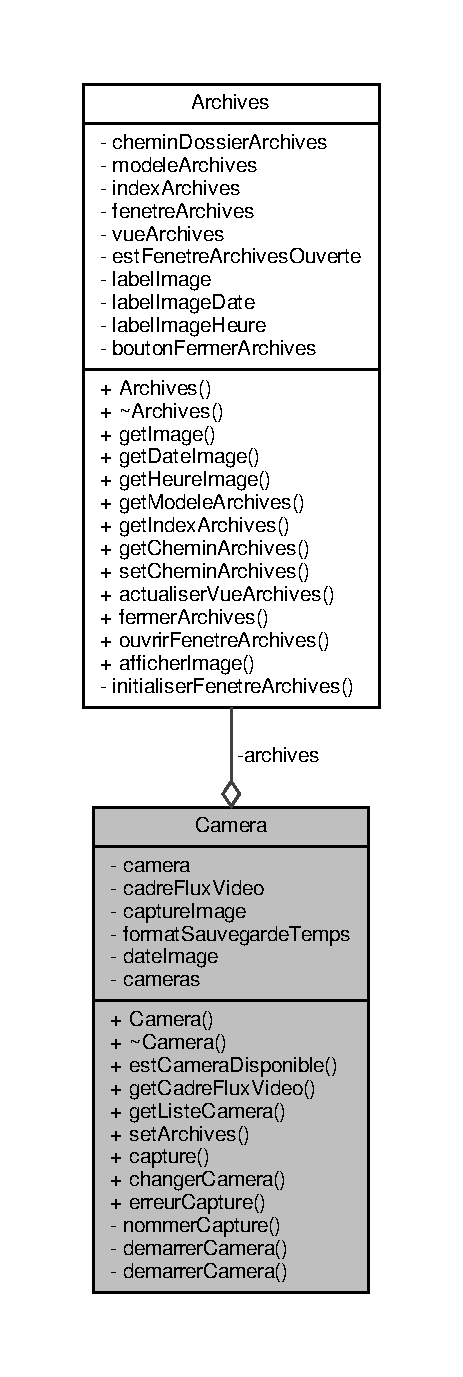
\includegraphics[height=550pt]{class_camera__coll__graph}
\end{center}
\end{figure}
\subsubsection*{Connecteurs publics}
\begin{DoxyCompactItemize}
\item 
void \hyperlink{class_camera_a3ca730dcbd7ea6bfba12931a15066f6c}{capture} ()
\begin{DoxyCompactList}\small\item\em Capture l\textquotesingle{}image du flux video. \end{DoxyCompactList}\item 
void \hyperlink{class_camera_a82a0dd06f1802dc0ec0ea8ff6fcbd231}{changer\+Camera} (Q\+String)
\begin{DoxyCompactList}\small\item\em Permet de démarrer le flux vidéo de la caméra choisir dans le Q\+Combo\+Box sur l\textquotesingle{}I\+HM. \end{DoxyCompactList}\item 
void \hyperlink{class_camera_ac5b8c16f8edcb92569fab87185fc0500}{erreur\+Capture} (int id, Q\+Camera\+Image\+Capture\+::\+Error error, const Q\+String \&error\+String)
\end{DoxyCompactItemize}
\subsubsection*{Fonctions membres publiques}
\begin{DoxyCompactItemize}
\item 
\hyperlink{class_camera_ae3aa4afd7a3d9ddc2bf710bc74dc293e}{Camera} (Q\+Object $\ast$parent=nullptr)
\item 
\hyperlink{class_camera_ad1897942d0ccf91052386388a497349f}{$\sim$\+Camera} ()
\item 
bool \hyperlink{class_camera_afb73ab859802a143a1a00443e396143e}{est\+Camera\+Disponible} ()
\begin{DoxyCompactList}\small\item\em Retourne un booléen sur l\textquotesingle{}état de disponibilité de la caméra. \end{DoxyCompactList}\item 
Q\+Camera\+Viewfinder $\ast$ \hyperlink{class_camera_a67420d3ef14065a412327ada6193a2e0}{get\+Cadre\+Flux\+Video} ()
\begin{DoxyCompactList}\small\item\em retourne le flux video \end{DoxyCompactList}\item 
Q\+List$<$ Q\+Camera\+Info $>$ \hyperlink{class_camera_ad8a2a21d3701375a553c7c90646c694f}{get\+Liste\+Camera} ()
\begin{DoxyCompactList}\small\item\em retourne toute les caméras disponible \end{DoxyCompactList}\item 
void \hyperlink{class_camera_a66b844eec2b721a6ac23b80cb3fe2426}{set\+Archives} (\hyperlink{class_archives}{Archives} $\ast$\hyperlink{class_camera_a5eb3a29aeeab2f2755d0b69ac7cf550a}{archives})
\end{DoxyCompactItemize}
\subsubsection*{Fonctions membres privées}
\begin{DoxyCompactItemize}
\item 
Q\+String \hyperlink{class_camera_a60d2c9f16b6f235ab6dd0360c883e0d0}{nommer\+Capture} ()
\begin{DoxyCompactList}\small\item\em Renomme la photo capturée au format \+: \char`\"{}yyyy-\/\+M\+M-\/dd\+\_\+\+H\+H\+:mm\+:ss\char`\"{}. \end{DoxyCompactList}\item 
void \hyperlink{class_camera_a181773c87c3deaea9fa9844f8ac294e3}{demarrer\+Camera} ()
\item 
void \hyperlink{class_camera_a7eb23e1a5fe67c61f36b8a97ff1f882c}{demarrer\+Camera} (Q\+Camera\+Info)
\begin{DoxyCompactList}\small\item\em Demarre le retour vidéo sur l\textquotesingle{}I\+HM. \end{DoxyCompactList}\end{DoxyCompactItemize}
\subsubsection*{Attributs privés}
\begin{DoxyCompactItemize}
\item 
Q\+Camera $\ast$ \hyperlink{class_camera_a282a199ddd33fe64bc27b32a55719054}{camera}
\begin{DoxyCompactList}\small\item\em Permet la connexion avec la caméra. \end{DoxyCompactList}\item 
\hyperlink{class_archives}{Archives} $\ast$ \hyperlink{class_camera_a5eb3a29aeeab2f2755d0b69ac7cf550a}{archives}
\begin{DoxyCompactList}\small\item\em Permet la connexion avec les archives. \end{DoxyCompactList}\item 
Q\+Camera\+Viewfinder $\ast$ \hyperlink{class_camera_abf5fd38d19f0f06dfd7ec9e37f73adb8}{cadre\+Flux\+Video}
\begin{DoxyCompactList}\small\item\em Permet l\textquotesingle{}affichage du flux vidéo. \end{DoxyCompactList}\item 
Q\+Camera\+Image\+Capture $\ast$ \hyperlink{class_camera_a482276c4fd0ba7172670006556322b62}{capture\+Image}
\begin{DoxyCompactList}\small\item\em Permet la capture d\textquotesingle{}image. \end{DoxyCompactList}\item 
Q\+String \hyperlink{class_camera_a1056fa6cffd2914d9e5a171bebf5ba7e}{format\+Sauvegarde\+Temps}
\begin{DoxyCompactList}\small\item\em Le format de sauvegarde du temps pour l\textquotesingle{}archivages. \end{DoxyCompactList}\item 
Q\+String \hyperlink{class_camera_a4433c250847de630592927b6c034f3c8}{date\+Image}
\begin{DoxyCompactList}\small\item\em Stock la date de la prise de photo pour l\textquotesingle{}archivage. \end{DoxyCompactList}\item 
Q\+List$<$ Q\+Camera\+Info $>$ \hyperlink{class_camera_a3bea5177e857533a53cb94135bee8c6b}{cameras}
\begin{DoxyCompactList}\small\item\em Stock la liste des caméras disponibles. \end{DoxyCompactList}\end{DoxyCompactItemize}


\subsubsection{Description détaillée}
\begin{DoxyAuthor}{Auteur}
Nicolas B\+O\+F\+F\+R\+E\+DO
\end{DoxyAuthor}
\begin{DoxyVersion}{Version}
1.\+1
\end{DoxyVersion}
\begin{DoxyDate}{Date}
Jeudi 13 Juin 2019 
\end{DoxyDate}


\subsubsection{Documentation des constructeurs et destructeur}
\mbox{\Hypertarget{class_camera_ae3aa4afd7a3d9ddc2bf710bc74dc293e}\label{class_camera_ae3aa4afd7a3d9ddc2bf710bc74dc293e}} 
\index{Camera@{Camera}!Camera@{Camera}}
\index{Camera@{Camera}!Camera@{Camera}}
\paragraph{\texorpdfstring{Camera()}{Camera()}}
{\footnotesize\ttfamily Camera\+::\+Camera (\begin{DoxyParamCaption}\item[{Q\+Object $\ast$}]{parent = {\ttfamily nullptr} }\end{DoxyParamCaption})}



Références \hyperlink{class_camera_abf5fd38d19f0f06dfd7ec9e37f73adb8}{cadre\+Flux\+Video}, \hyperlink{class_camera_a282a199ddd33fe64bc27b32a55719054}{camera}, \hyperlink{class_camera_a3bea5177e857533a53cb94135bee8c6b}{cameras}, \hyperlink{class_camera_a482276c4fd0ba7172670006556322b62}{capture\+Image}, \hyperlink{class_camera_a181773c87c3deaea9fa9844f8ac294e3}{demarrer\+Camera()}, et \hyperlink{class_camera_afb73ab859802a143a1a00443e396143e}{est\+Camera\+Disponible()}.


\begin{DoxyCode}
00022                               : QObject(parent),
00023   \hyperlink{class_camera_a282a199ddd33fe64bc27b32a55719054}{camera}(\textcolor{keyword}{nullptr}),
00024   \hyperlink{class_camera_a5eb3a29aeeab2f2755d0b69ac7cf550a}{archives}(\textcolor{keyword}{nullptr}),
00025   \hyperlink{class_camera_abf5fd38d19f0f06dfd7ec9e37f73adb8}{cadreFluxVideo}(\textcolor{keyword}{nullptr}),
00026   \hyperlink{class_camera_a482276c4fd0ba7172670006556322b62}{captureImage}(\textcolor{keyword}{nullptr}),
00027   \hyperlink{class_camera_a1056fa6cffd2914d9e5a171bebf5ba7e}{formatSauvegardeTemps}(\textcolor{stringliteral}{"dd-MM-yyyy\_HH:mm:ss"})
00028 \{
00029     \hyperlink{class_camera_abf5fd38d19f0f06dfd7ec9e37f73adb8}{cadreFluxVideo} = \textcolor{keyword}{new} QCameraViewfinder;
00030     \hyperlink{class_camera_a282a199ddd33fe64bc27b32a55719054}{camera} = \textcolor{keyword}{new} QCamera;
00031     \hyperlink{class_camera_a482276c4fd0ba7172670006556322b62}{captureImage} = \textcolor{keyword}{new} QCameraImageCapture(\hyperlink{class_camera_a282a199ddd33fe64bc27b32a55719054}{camera});
00032     \hyperlink{class_camera_a3bea5177e857533a53cb94135bee8c6b}{cameras} = QCameraInfo::availableCameras();
00033 
00034     \textcolor{keywordflow}{if}(\hyperlink{class_camera_afb73ab859802a143a1a00443e396143e}{estCameraDisponible}())
00035         \hyperlink{class_camera_a181773c87c3deaea9fa9844f8ac294e3}{demarrerCamera}(\hyperlink{class_camera_a3bea5177e857533a53cb94135bee8c6b}{cameras}[0]);
00036 
00037     qDebug() << Q\_FUNC\_INFO << \hyperlink{class_camera_a3bea5177e857533a53cb94135bee8c6b}{cameras};
00038 \}
\end{DoxyCode}
\mbox{\Hypertarget{class_camera_ad1897942d0ccf91052386388a497349f}\label{class_camera_ad1897942d0ccf91052386388a497349f}} 
\index{Camera@{Camera}!````~Camera@{$\sim$\+Camera}}
\index{````~Camera@{$\sim$\+Camera}!Camera@{Camera}}
\paragraph{\texorpdfstring{$\sim$\+Camera()}{~Camera()}}
{\footnotesize\ttfamily Camera\+::$\sim$\+Camera (\begin{DoxyParamCaption}{ }\end{DoxyParamCaption})}



Références \hyperlink{class_camera_abf5fd38d19f0f06dfd7ec9e37f73adb8}{cadre\+Flux\+Video}, et \hyperlink{class_camera_a282a199ddd33fe64bc27b32a55719054}{camera}.


\begin{DoxyCode}
00041 \{
00042     \textcolor{keyword}{delete} \hyperlink{class_camera_abf5fd38d19f0f06dfd7ec9e37f73adb8}{cadreFluxVideo};
00043     \textcolor{keyword}{delete} \hyperlink{class_camera_a282a199ddd33fe64bc27b32a55719054}{camera};
00044     qDebug() << Q\_FUNC\_INFO;
00045 \}
\end{DoxyCode}


\subsubsection{Documentation des fonctions membres}
\mbox{\Hypertarget{class_camera_a3ca730dcbd7ea6bfba12931a15066f6c}\label{class_camera_a3ca730dcbd7ea6bfba12931a15066f6c}} 
\index{Camera@{Camera}!capture@{capture}}
\index{capture@{capture}!Camera@{Camera}}
\paragraph{\texorpdfstring{capture}{capture}}
{\footnotesize\ttfamily void Camera\+::capture (\begin{DoxyParamCaption}{ }\end{DoxyParamCaption})\hspace{0.3cm}{\ttfamily [slot]}}



Références \hyperlink{class_camera_a482276c4fd0ba7172670006556322b62}{capture\+Image}, et \hyperlink{class_camera_a60d2c9f16b6f235ab6dd0360c883e0d0}{nommer\+Capture()}.


\begin{DoxyCode}
00116 \{
00117     qDebug() << Q\_FUNC\_INFO;
00118     QString nomCapture = this->\hyperlink{class_camera_a60d2c9f16b6f235ab6dd0360c883e0d0}{nommerCapture}();
00119     qDebug() << Q\_FUNC\_INFO << \textcolor{stringliteral}{"nomCapture"} << nomCapture;
00120     \hyperlink{class_camera_a482276c4fd0ba7172670006556322b62}{captureImage}->capture(nomCapture);
00121 \}
\end{DoxyCode}
\mbox{\Hypertarget{class_camera_a82a0dd06f1802dc0ec0ea8ff6fcbd231}\label{class_camera_a82a0dd06f1802dc0ec0ea8ff6fcbd231}} 
\index{Camera@{Camera}!changer\+Camera@{changer\+Camera}}
\index{changer\+Camera@{changer\+Camera}!Camera@{Camera}}
\paragraph{\texorpdfstring{changer\+Camera}{changerCamera}}
{\footnotesize\ttfamily void Camera\+::changer\+Camera (\begin{DoxyParamCaption}\item[{Q\+String}]{nom\+Camera }\end{DoxyParamCaption})\hspace{0.3cm}{\ttfamily [slot]}}


\begin{DoxyParams}{Paramètres}
{\em nom\+Camera} & Un {\itshape Q\+String}, le nom de la caméra \\
\hline
\end{DoxyParams}


Références \hyperlink{class_camera_a3bea5177e857533a53cb94135bee8c6b}{cameras}, et \hyperlink{class_camera_a181773c87c3deaea9fa9844f8ac294e3}{demarrer\+Camera()}.


\begin{DoxyCode}
00142 \{
00143     QString cameraTrouvee;
00144     QList<QCameraInfo> \hyperlink{class_camera_a3bea5177e857533a53cb94135bee8c6b}{cameras} = QCameraInfo::availableCameras();
00145     \textcolor{keywordflow}{foreach} (\textcolor{keyword}{const} QCameraInfo &cameraInfo, cameras)
00146     \{
00147         cameraTrouvee = cameraInfo.description() + \textcolor{stringliteral}{" ("} + cameraInfo.deviceName()+ \textcolor{stringliteral}{")"};
00148         \textcolor{keywordflow}{if} (cameraTrouvee == nomCamera)
00149         \{
00150             this->\hyperlink{class_camera_a181773c87c3deaea9fa9844f8ac294e3}{demarrerCamera}(cameraInfo);
00151         \}
00152     \}
00153 \}
\end{DoxyCode}
\mbox{\Hypertarget{class_camera_a181773c87c3deaea9fa9844f8ac294e3}\label{class_camera_a181773c87c3deaea9fa9844f8ac294e3}} 
\index{Camera@{Camera}!demarrer\+Camera@{demarrer\+Camera}}
\index{demarrer\+Camera@{demarrer\+Camera}!Camera@{Camera}}
\paragraph{\texorpdfstring{demarrer\+Camera()}{demarrerCamera()}\hspace{0.1cm}{\footnotesize\ttfamily [1/2]}}
{\footnotesize\ttfamily void Camera\+::demarrer\+Camera (\begin{DoxyParamCaption}{ }\end{DoxyParamCaption})\hspace{0.3cm}{\ttfamily [private]}}



Référencé par \hyperlink{class_camera_ae3aa4afd7a3d9ddc2bf710bc74dc293e}{Camera()}, et \hyperlink{class_camera_a82a0dd06f1802dc0ec0ea8ff6fcbd231}{changer\+Camera()}.

\mbox{\Hypertarget{class_camera_a7eb23e1a5fe67c61f36b8a97ff1f882c}\label{class_camera_a7eb23e1a5fe67c61f36b8a97ff1f882c}} 
\index{Camera@{Camera}!demarrer\+Camera@{demarrer\+Camera}}
\index{demarrer\+Camera@{demarrer\+Camera}!Camera@{Camera}}
\paragraph{\texorpdfstring{demarrer\+Camera()}{demarrerCamera()}\hspace{0.1cm}{\footnotesize\ttfamily [2/2]}}
{\footnotesize\ttfamily void Camera\+::demarrer\+Camera (\begin{DoxyParamCaption}\item[{Q\+Camera\+Info}]{camera\+Selectionnee }\end{DoxyParamCaption})\hspace{0.3cm}{\ttfamily [private]}}

Par défaut la méthode reçoit la première caméra trouvée 
\begin{DoxyParams}{Paramètres}
{\em camera\+Selectionnee} & \\
\hline
\end{DoxyParams}


Références \hyperlink{class_camera_abf5fd38d19f0f06dfd7ec9e37f73adb8}{cadre\+Flux\+Video}, \hyperlink{class_camera_a282a199ddd33fe64bc27b32a55719054}{camera}, \hyperlink{class_camera_a482276c4fd0ba7172670006556322b62}{capture\+Image}, \hyperlink{class_camera_ac5b8c16f8edcb92569fab87185fc0500}{erreur\+Capture()}, et \hyperlink{class_camera_afb73ab859802a143a1a00443e396143e}{est\+Camera\+Disponible()}.


\begin{DoxyCode}
00092 \{
00093     \textcolor{keywordflow}{if}(\hyperlink{class_camera_a282a199ddd33fe64bc27b32a55719054}{camera} != \textcolor{keyword}{nullptr})
00094         \textcolor{keyword}{delete} \hyperlink{class_camera_a282a199ddd33fe64bc27b32a55719054}{camera};
00095     \textcolor{keywordflow}{if}(\hyperlink{class_camera_a482276c4fd0ba7172670006556322b62}{captureImage} != \textcolor{keyword}{nullptr})
00096         \textcolor{keyword}{delete} \hyperlink{class_camera_a482276c4fd0ba7172670006556322b62}{captureImage};
00097 
00098     \textcolor{keywordflow}{if}(\hyperlink{class_camera_afb73ab859802a143a1a00443e396143e}{estCameraDisponible}())
00099     \{
00100         qDebug() << Q\_FUNC\_INFO << \textcolor{stringliteral}{"cameraSelectionnee"} << cameraSelectionnee.deviceName();
00101         \hyperlink{class_camera_a282a199ddd33fe64bc27b32a55719054}{camera} = \textcolor{keyword}{new} QCamera(cameraSelectionnee);
00102         \hyperlink{class_camera_a282a199ddd33fe64bc27b32a55719054}{camera}->setViewfinder(\hyperlink{class_camera_abf5fd38d19f0f06dfd7ec9e37f73adb8}{cadreFluxVideo});
00103         \hyperlink{class_camera_a282a199ddd33fe64bc27b32a55719054}{camera}->setCaptureMode(QCamera::CaptureStillImage);
00104         \hyperlink{class_camera_a482276c4fd0ba7172670006556322b62}{captureImage} = \textcolor{keyword}{new} QCameraImageCapture(\hyperlink{class_camera_a282a199ddd33fe64bc27b32a55719054}{camera});
00105         \hyperlink{class_camera_a482276c4fd0ba7172670006556322b62}{captureImage}->setCaptureDestination(QCameraImageCapture::CaptureToBuffer);
00106         connect(\hyperlink{class_camera_a482276c4fd0ba7172670006556322b62}{captureImage}, SIGNAL(error(\textcolor{keywordtype}{int},QCameraImageCapture::Error,QString)), \textcolor{keyword}{this}, SLOT
      (\hyperlink{class_camera_ac5b8c16f8edcb92569fab87185fc0500}{erreurCapture}(\textcolor{keywordtype}{int},QCameraImageCapture::Error,QString)));
00107 
00108         \hyperlink{class_camera_a282a199ddd33fe64bc27b32a55719054}{camera}->start();
00109     \}
00110 \}
\end{DoxyCode}
\mbox{\Hypertarget{class_camera_ac5b8c16f8edcb92569fab87185fc0500}\label{class_camera_ac5b8c16f8edcb92569fab87185fc0500}} 
\index{Camera@{Camera}!erreur\+Capture@{erreur\+Capture}}
\index{erreur\+Capture@{erreur\+Capture}!Camera@{Camera}}
\paragraph{\texorpdfstring{erreur\+Capture}{erreurCapture}}
{\footnotesize\ttfamily void Camera\+::erreur\+Capture (\begin{DoxyParamCaption}\item[{int}]{id,  }\item[{Q\+Camera\+Image\+Capture\+::\+Error}]{error,  }\item[{const Q\+String \&}]{error\+String }\end{DoxyParamCaption})\hspace{0.3cm}{\ttfamily [slot]}}



Référencé par \hyperlink{class_camera_a7eb23e1a5fe67c61f36b8a97ff1f882c}{demarrer\+Camera()}.


\begin{DoxyCode}
00156 \{
00157     Q\_UNUSED(\textcolor{keywordtype}{id})
00158     Q\_UNUSED(error)
00159     qDebug() << Q\_FUNC\_INFO << errorString;
00160 \}
\end{DoxyCode}
\mbox{\Hypertarget{class_camera_afb73ab859802a143a1a00443e396143e}\label{class_camera_afb73ab859802a143a1a00443e396143e}} 
\index{Camera@{Camera}!est\+Camera\+Disponible@{est\+Camera\+Disponible}}
\index{est\+Camera\+Disponible@{est\+Camera\+Disponible}!Camera@{Camera}}
\paragraph{\texorpdfstring{est\+Camera\+Disponible()}{estCameraDisponible()}}
{\footnotesize\ttfamily bool Camera\+::est\+Camera\+Disponible (\begin{DoxyParamCaption}{ }\end{DoxyParamCaption})}

\begin{DoxyReturn}{Renvoie}
Un {\itshape booléen}, vrai si la caméra est disponible, faux sinon. 
\end{DoxyReturn}


Références \hyperlink{class_camera_a3bea5177e857533a53cb94135bee8c6b}{cameras}.



Référencé par \hyperlink{class_i_h_m_rov_abbfcdc154a6ae7f941d186f6c90a5a2b}{I\+H\+M\+Rov\+::actualise\+Icones\+Etat()}, \hyperlink{class_camera_ae3aa4afd7a3d9ddc2bf710bc74dc293e}{Camera()}, et \hyperlink{class_camera_a7eb23e1a5fe67c61f36b8a97ff1f882c}{demarrer\+Camera()}.


\begin{DoxyCode}
00052 \{
00053     \textcolor{keywordflow}{if} (\hyperlink{class_camera_a3bea5177e857533a53cb94135bee8c6b}{cameras}.count() > 0)
00054         \textcolor{keywordflow}{return} \textcolor{keyword}{true};
00055 
00056     \textcolor{keywordflow}{else}
00057         \textcolor{keywordflow}{return} \textcolor{keyword}{false};
00058 \}
\end{DoxyCode}
\mbox{\Hypertarget{class_camera_a67420d3ef14065a412327ada6193a2e0}\label{class_camera_a67420d3ef14065a412327ada6193a2e0}} 
\index{Camera@{Camera}!get\+Cadre\+Flux\+Video@{get\+Cadre\+Flux\+Video}}
\index{get\+Cadre\+Flux\+Video@{get\+Cadre\+Flux\+Video}!Camera@{Camera}}
\paragraph{\texorpdfstring{get\+Cadre\+Flux\+Video()}{getCadreFluxVideo()}}
{\footnotesize\ttfamily Q\+Camera\+Viewfinder $\ast$ Camera\+::get\+Cadre\+Flux\+Video (\begin{DoxyParamCaption}{ }\end{DoxyParamCaption})}

Un assesseur permettant d\textquotesingle{}avoir le retour vidéo 

Références \hyperlink{class_camera_abf5fd38d19f0f06dfd7ec9e37f73adb8}{cadre\+Flux\+Video}.



Référencé par \hyperlink{class_i_h_m_rov_a5dac1fb4612866cc61f699a415e0ef6b}{I\+H\+M\+Rov\+::\+I\+H\+M\+Rov()}.


\begin{DoxyCode}
00082 \{
00083     \textcolor{keywordflow}{return} \hyperlink{class_camera_abf5fd38d19f0f06dfd7ec9e37f73adb8}{cadreFluxVideo};
00084 \}
\end{DoxyCode}
\mbox{\Hypertarget{class_camera_ad8a2a21d3701375a553c7c90646c694f}\label{class_camera_ad8a2a21d3701375a553c7c90646c694f}} 
\index{Camera@{Camera}!get\+Liste\+Camera@{get\+Liste\+Camera}}
\index{get\+Liste\+Camera@{get\+Liste\+Camera}!Camera@{Camera}}
\paragraph{\texorpdfstring{get\+Liste\+Camera()}{getListeCamera()}}
{\footnotesize\ttfamily Q\+List$<$ Q\+Camera\+Info $>$ Camera\+::get\+Liste\+Camera (\begin{DoxyParamCaption}{ }\end{DoxyParamCaption})}



Références \hyperlink{class_camera_a3bea5177e857533a53cb94135bee8c6b}{cameras}.



Référencé par \hyperlink{class_i_h_m_rov_af3e46f174ab2fdeaebb2d00e6b8bcb33}{I\+H\+M\+Rov\+::initialiser\+Liste\+Camera()}.


\begin{DoxyCode}
00063 \{
00064     QList<QCameraInfo> listeCamera;
00065     \textcolor{keywordflow}{foreach} (\textcolor{keyword}{const} QCameraInfo &cameraInfo, \hyperlink{class_camera_a3bea5177e857533a53cb94135bee8c6b}{cameras})
00066     \{
00067         listeCamera.append(cameraInfo);
00068     \}
00069     \textcolor{keywordflow}{return} listeCamera;
00070 \}
\end{DoxyCode}
\mbox{\Hypertarget{class_camera_a60d2c9f16b6f235ab6dd0360c883e0d0}\label{class_camera_a60d2c9f16b6f235ab6dd0360c883e0d0}} 
\index{Camera@{Camera}!nommer\+Capture@{nommer\+Capture}}
\index{nommer\+Capture@{nommer\+Capture}!Camera@{Camera}}
\paragraph{\texorpdfstring{nommer\+Capture()}{nommerCapture()}}
{\footnotesize\ttfamily Q\+String Camera\+::nommer\+Capture (\begin{DoxyParamCaption}{ }\end{DoxyParamCaption})\hspace{0.3cm}{\ttfamily [private]}}

Indique le chemin vers un dossier de stockage des photos, à l\textquotesingle{}emplacement de l\textquotesingle{}éxécutable. 

Références \hyperlink{class_camera_a5eb3a29aeeab2f2755d0b69ac7cf550a}{archives}, \hyperlink{class_camera_a4433c250847de630592927b6c034f3c8}{date\+Image}, \hyperlink{class_camera_a1056fa6cffd2914d9e5a171bebf5ba7e}{format\+Sauvegarde\+Temps}, et \hyperlink{class_archives_a65dfbaba0123e6530b03bfb70e614c90}{Archives\+::get\+Chemin\+Archives()}.



Référencé par \hyperlink{class_camera_a3ca730dcbd7ea6bfba12931a15066f6c}{capture()}.


\begin{DoxyCode}
00128 \{
00129     QString nom = QApplication::applicationDirPath() + \textcolor{stringliteral}{"/defaut"};
00130     QDateTime dateCapture = QDateTime::currentDateTime();
00131     \hyperlink{class_camera_a4433c250847de630592927b6c034f3c8}{dateImage} = dateCapture.toString(\hyperlink{class_camera_a1056fa6cffd2914d9e5a171bebf5ba7e}{formatSauvegardeTemps});
00132     nom = \hyperlink{class_camera_a5eb3a29aeeab2f2755d0b69ac7cf550a}{archives}->\hyperlink{class_archives_a65dfbaba0123e6530b03bfb70e614c90}{getCheminArchives}() + \textcolor{stringliteral}{"/"} + 
      \hyperlink{class_camera_a4433c250847de630592927b6c034f3c8}{dateImage};
00133     qDebug() << Q\_FUNC\_INFO << nom;
00134     \textcolor{keywordflow}{return} nom;
00135 \}
\end{DoxyCode}
\mbox{\Hypertarget{class_camera_a66b844eec2b721a6ac23b80cb3fe2426}\label{class_camera_a66b844eec2b721a6ac23b80cb3fe2426}} 
\index{Camera@{Camera}!set\+Archives@{set\+Archives}}
\index{set\+Archives@{set\+Archives}!Camera@{Camera}}
\paragraph{\texorpdfstring{set\+Archives()}{setArchives()}}
{\footnotesize\ttfamily void Camera\+::set\+Archives (\begin{DoxyParamCaption}\item[{\hyperlink{class_archives}{Archives} $\ast$}]{archives }\end{DoxyParamCaption})}



Références \hyperlink{class_camera_a5eb3a29aeeab2f2755d0b69ac7cf550a}{archives}.



Référencé par \hyperlink{class_i_h_m_rov_a5dac1fb4612866cc61f699a415e0ef6b}{I\+H\+M\+Rov\+::\+I\+H\+M\+Rov()}.


\begin{DoxyCode}
00073 \{
00074     this->archives = \hyperlink{class_camera_a5eb3a29aeeab2f2755d0b69ac7cf550a}{archives};
00075 \}
\end{DoxyCode}


\subsubsection{Documentation des données membres}
\mbox{\Hypertarget{class_camera_a5eb3a29aeeab2f2755d0b69ac7cf550a}\label{class_camera_a5eb3a29aeeab2f2755d0b69ac7cf550a}} 
\index{Camera@{Camera}!archives@{archives}}
\index{archives@{archives}!Camera@{Camera}}
\paragraph{\texorpdfstring{archives}{archives}}
{\footnotesize\ttfamily \hyperlink{class_archives}{Archives}$\ast$ Camera\+::archives\hspace{0.3cm}{\ttfamily [private]}}



Référencé par \hyperlink{class_camera_a60d2c9f16b6f235ab6dd0360c883e0d0}{nommer\+Capture()}, et \hyperlink{class_camera_a66b844eec2b721a6ac23b80cb3fe2426}{set\+Archives()}.

\mbox{\Hypertarget{class_camera_abf5fd38d19f0f06dfd7ec9e37f73adb8}\label{class_camera_abf5fd38d19f0f06dfd7ec9e37f73adb8}} 
\index{Camera@{Camera}!cadre\+Flux\+Video@{cadre\+Flux\+Video}}
\index{cadre\+Flux\+Video@{cadre\+Flux\+Video}!Camera@{Camera}}
\paragraph{\texorpdfstring{cadre\+Flux\+Video}{cadreFluxVideo}}
{\footnotesize\ttfamily Q\+Camera\+Viewfinder$\ast$ Camera\+::cadre\+Flux\+Video\hspace{0.3cm}{\ttfamily [private]}}



Référencé par \hyperlink{class_camera_ae3aa4afd7a3d9ddc2bf710bc74dc293e}{Camera()}, \hyperlink{class_camera_a7eb23e1a5fe67c61f36b8a97ff1f882c}{demarrer\+Camera()}, \hyperlink{class_camera_a67420d3ef14065a412327ada6193a2e0}{get\+Cadre\+Flux\+Video()}, et \hyperlink{class_camera_ad1897942d0ccf91052386388a497349f}{$\sim$\+Camera()}.

\mbox{\Hypertarget{class_camera_a282a199ddd33fe64bc27b32a55719054}\label{class_camera_a282a199ddd33fe64bc27b32a55719054}} 
\index{Camera@{Camera}!camera@{camera}}
\index{camera@{camera}!Camera@{Camera}}
\paragraph{\texorpdfstring{camera}{camera}}
{\footnotesize\ttfamily Q\+Camera$\ast$ Camera\+::camera\hspace{0.3cm}{\ttfamily [private]}}



Référencé par \hyperlink{class_camera_ae3aa4afd7a3d9ddc2bf710bc74dc293e}{Camera()}, \hyperlink{class_camera_a7eb23e1a5fe67c61f36b8a97ff1f882c}{demarrer\+Camera()}, et \hyperlink{class_camera_ad1897942d0ccf91052386388a497349f}{$\sim$\+Camera()}.

\mbox{\Hypertarget{class_camera_a3bea5177e857533a53cb94135bee8c6b}\label{class_camera_a3bea5177e857533a53cb94135bee8c6b}} 
\index{Camera@{Camera}!cameras@{cameras}}
\index{cameras@{cameras}!Camera@{Camera}}
\paragraph{\texorpdfstring{cameras}{cameras}}
{\footnotesize\ttfamily Q\+List$<$Q\+Camera\+Info$>$ Camera\+::cameras\hspace{0.3cm}{\ttfamily [private]}}



Référencé par \hyperlink{class_camera_ae3aa4afd7a3d9ddc2bf710bc74dc293e}{Camera()}, \hyperlink{class_camera_a82a0dd06f1802dc0ec0ea8ff6fcbd231}{changer\+Camera()}, \hyperlink{class_camera_afb73ab859802a143a1a00443e396143e}{est\+Camera\+Disponible()}, et \hyperlink{class_camera_ad8a2a21d3701375a553c7c90646c694f}{get\+Liste\+Camera()}.

\mbox{\Hypertarget{class_camera_a482276c4fd0ba7172670006556322b62}\label{class_camera_a482276c4fd0ba7172670006556322b62}} 
\index{Camera@{Camera}!capture\+Image@{capture\+Image}}
\index{capture\+Image@{capture\+Image}!Camera@{Camera}}
\paragraph{\texorpdfstring{capture\+Image}{captureImage}}
{\footnotesize\ttfamily Q\+Camera\+Image\+Capture$\ast$ Camera\+::capture\+Image\hspace{0.3cm}{\ttfamily [private]}}



Référencé par \hyperlink{class_camera_ae3aa4afd7a3d9ddc2bf710bc74dc293e}{Camera()}, \hyperlink{class_camera_a3ca730dcbd7ea6bfba12931a15066f6c}{capture()}, et \hyperlink{class_camera_a7eb23e1a5fe67c61f36b8a97ff1f882c}{demarrer\+Camera()}.

\mbox{\Hypertarget{class_camera_a4433c250847de630592927b6c034f3c8}\label{class_camera_a4433c250847de630592927b6c034f3c8}} 
\index{Camera@{Camera}!date\+Image@{date\+Image}}
\index{date\+Image@{date\+Image}!Camera@{Camera}}
\paragraph{\texorpdfstring{date\+Image}{dateImage}}
{\footnotesize\ttfamily Q\+String Camera\+::date\+Image\hspace{0.3cm}{\ttfamily [private]}}



Référencé par \hyperlink{class_camera_a60d2c9f16b6f235ab6dd0360c883e0d0}{nommer\+Capture()}.

\mbox{\Hypertarget{class_camera_a1056fa6cffd2914d9e5a171bebf5ba7e}\label{class_camera_a1056fa6cffd2914d9e5a171bebf5ba7e}} 
\index{Camera@{Camera}!format\+Sauvegarde\+Temps@{format\+Sauvegarde\+Temps}}
\index{format\+Sauvegarde\+Temps@{format\+Sauvegarde\+Temps}!Camera@{Camera}}
\paragraph{\texorpdfstring{format\+Sauvegarde\+Temps}{formatSauvegardeTemps}}
{\footnotesize\ttfamily Q\+String Camera\+::format\+Sauvegarde\+Temps\hspace{0.3cm}{\ttfamily [private]}}



Référencé par \hyperlink{class_camera_a60d2c9f16b6f235ab6dd0360c883e0d0}{nommer\+Capture()}.



La documentation de cette classe a été générée à partir des fichiers suivants \+:\begin{DoxyCompactItemize}
\item 
\hyperlink{camera_8h}{camera.\+h}\item 
\hyperlink{camera_8cpp}{camera.\+cpp}\end{DoxyCompactItemize}

\hypertarget{class_communication_rov}{}\subsection{Référence de la classe Communication\+Rov}
\label{class_communication_rov}\index{Communication\+Rov@{Communication\+Rov}}


Déclaration de la classe \hyperlink{class_communication_rov}{Communication\+Rov}. Gère la communication entre le \hyperlink{class_rov}{Rov} et le \hyperlink{class_rov}{Rov}.  




{\ttfamily \#include $<$communicationrov.\+h$>$}



Graphe de collaboration de Communication\+Rov\+:
\nopagebreak
\begin{figure}[H]
\begin{center}
\leavevmode
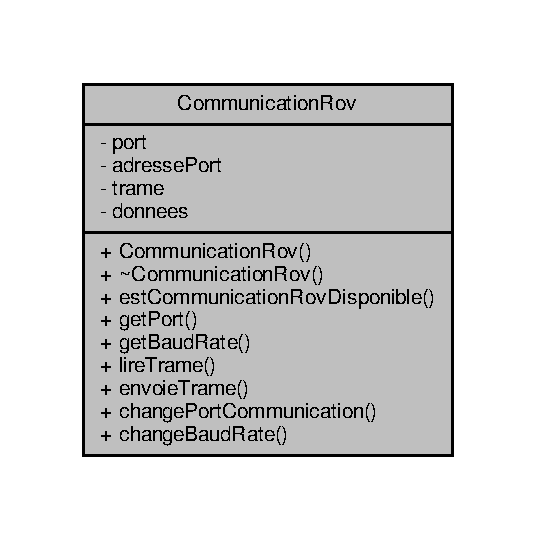
\includegraphics[width=257pt]{class_communication_rov__coll__graph}
\end{center}
\end{figure}
\subsubsection*{Connecteurs publics}
\begin{DoxyCompactItemize}
\item 
void \hyperlink{class_communication_rov_a5822d2f41553221ea876ea09e148f859}{lire\+Trame} ()
\begin{DoxyCompactList}\small\item\em Récupère la trame envoyée par le \hyperlink{class_rov}{Rov}, et la renvoie sous un signal si cette dernière est complète. \end{DoxyCompactList}\item 
bool \hyperlink{class_communication_rov_ac243fcfb073f4ceaf58fab1d41207801}{envoie\+Trame} (Q\+String \hyperlink{class_communication_rov_a7100b1be33860d235b45efd9010ac218}{trame})
\begin{DoxyCompactList}\small\item\em Envoie une trame au \hyperlink{class_rov}{Rov}. \end{DoxyCompactList}\item 
void \hyperlink{class_communication_rov_ad46397a58ba7704fbd5ac5748e083004}{change\+Port\+Communication} (Q\+String nouveau\+Port)
\begin{DoxyCompactList}\small\item\em Modifie le port de communication du rov. \end{DoxyCompactList}\item 
void \hyperlink{class_communication_rov_ac49ffc6f2e6ae22ea9f99e10ca0a4163}{change\+Baud\+Rate} (Q\+String nouveau\+Baud\+Rate)
\begin{DoxyCompactList}\small\item\em Modifie le baudrate utilisé. \end{DoxyCompactList}\end{DoxyCompactItemize}
\subsubsection*{Signaux}
\begin{DoxyCompactItemize}
\item 
void \hyperlink{class_communication_rov_add205822378629204a4ee49ca74c6d56}{trame\+Recue} (Q\+String \hyperlink{class_communication_rov_a7100b1be33860d235b45efd9010ac218}{trame})
\begin{DoxyCompactList}\small\item\em Signal émis lorsque des nouvelles données ont été reçues. \end{DoxyCompactList}\end{DoxyCompactItemize}
\subsubsection*{Fonctions membres publiques}
\begin{DoxyCompactItemize}
\item 
\hyperlink{class_communication_rov_a22b64c69228d392a212f543e071adc02}{Communication\+Rov} (Q\+Object $\ast$parent=nullptr)
\item 
\hyperlink{class_communication_rov_a97e96f47dad6d47cbec4adc82756b49e}{$\sim$\+Communication\+Rov} ()
\item 
bool \hyperlink{class_communication_rov_a513c26b04745fa2ae31b4533d656dfd4}{est\+Communication\+Rov\+Disponible} ()
\begin{DoxyCompactList}\small\item\em Retourne l\textquotesingle{}é\&tat d\textquotesingle{}ouverture du port de communication vers le \hyperlink{class_rov}{Rov}. \end{DoxyCompactList}\item 
const Q\+String \hyperlink{class_communication_rov_a6226f9338fffc648cfca91c8e585a26b}{get\+Port} ()
\begin{DoxyCompactList}\small\item\em Retourne le port de communication utilisé. \end{DoxyCompactList}\item 
const Q\+String \hyperlink{class_communication_rov_a810de691dfc6d305f77c92ccd90bb6db}{get\+Baud\+Rate} ()
\begin{DoxyCompactList}\small\item\em Retourne le baudrate utilisé. \end{DoxyCompactList}\end{DoxyCompactItemize}
\subsubsection*{Attributs privés}
\begin{DoxyCompactItemize}
\item 
Q\+Serial\+Port $\ast$ \hyperlink{class_communication_rov_a21b62067ef0b2a6aec339df60b4abd72}{port}
\begin{DoxyCompactList}\small\item\em Port série pour la communication le programme et le \hyperlink{class_rov}{Rov}. \end{DoxyCompactList}\item 
Q\+String \hyperlink{class_communication_rov_a7bd5d36d065005b27ed6cb421c7ffe42}{adresse\+Port}
\begin{DoxyCompactList}\small\item\em Adresse du port de communication. \end{DoxyCompactList}\item 
Q\+String \hyperlink{class_communication_rov_a7100b1be33860d235b45efd9010ac218}{trame}
\begin{DoxyCompactList}\small\item\em Trame reçue par le port. \end{DoxyCompactList}\item 
Q\+Byte\+Array \hyperlink{class_communication_rov_acbb6939bb597179956c6f4bc5ca39f3f}{donnees}
\begin{DoxyCompactList}\small\item\em Dernière donnée reçue (ou en cours de réception) \end{DoxyCompactList}\end{DoxyCompactItemize}


\subsubsection{Description détaillée}
\begin{DoxyAuthor}{Auteur}
R\+E\+Y\+N\+I\+ER Jacques
\end{DoxyAuthor}
\begin{DoxyVersion}{Version}
1.\+1
\end{DoxyVersion}
\begin{DoxyDate}{Date}
Jeudi 13 Juin 2019 
\end{DoxyDate}


\subsubsection{Documentation des constructeurs et destructeur}
\mbox{\Hypertarget{class_communication_rov_a22b64c69228d392a212f543e071adc02}\label{class_communication_rov_a22b64c69228d392a212f543e071adc02}} 
\index{Communication\+Rov@{Communication\+Rov}!Communication\+Rov@{Communication\+Rov}}
\index{Communication\+Rov@{Communication\+Rov}!Communication\+Rov@{Communication\+Rov}}
\paragraph{\texorpdfstring{Communication\+Rov()}{CommunicationRov()}}
{\footnotesize\ttfamily Communication\+Rov\+::\+Communication\+Rov (\begin{DoxyParamCaption}\item[{Q\+Object $\ast$}]{parent = {\ttfamily nullptr} }\end{DoxyParamCaption})\hspace{0.3cm}{\ttfamily [explicit]}}



Références \hyperlink{class_communication_rov_a7bd5d36d065005b27ed6cb421c7ffe42}{adresse\+Port}, \hyperlink{class_communication_rov_a5822d2f41553221ea876ea09e148f859}{lire\+Trame()}, et \hyperlink{class_communication_rov_a21b62067ef0b2a6aec339df60b4abd72}{port}.


\begin{DoxyCode}
00017                                                   : QObject(parent), \hyperlink{class_communication_rov_a7bd5d36d065005b27ed6cb421c7ffe42}{adressePort}(\textcolor{stringliteral}{"/dev/ttyUSB0"})
00018 \{
00019     \hyperlink{class_communication_rov_a21b62067ef0b2a6aec339df60b4abd72}{port} = \textcolor{keyword}{new} QSerialPort(\hyperlink{class_communication_rov_a7bd5d36d065005b27ed6cb421c7ffe42}{adressePort});
00020 
00021     \hyperlink{class_communication_rov_a21b62067ef0b2a6aec339df60b4abd72}{port}->setBaudRate(QSerialPort::Baud38400);
00022 
00023     \hyperlink{class_communication_rov_a21b62067ef0b2a6aec339df60b4abd72}{port}->open(QIODevice::ReadWrite);
00024     qDebug() << Q\_FUNC\_INFO << \textcolor{stringliteral}{"Port ouvert :"} << \hyperlink{class_communication_rov_a21b62067ef0b2a6aec339df60b4abd72}{port}->isOpen();
00025 
00026     \textcolor{keywordflow}{if}(\hyperlink{class_communication_rov_a21b62067ef0b2a6aec339df60b4abd72}{port}->isOpen())
00027         connect(\hyperlink{class_communication_rov_a21b62067ef0b2a6aec339df60b4abd72}{port}, SIGNAL(readyRead()), \textcolor{keyword}{this}, SLOT(\hyperlink{class_communication_rov_a5822d2f41553221ea876ea09e148f859}{lireTrame}()));
00028 \}
\end{DoxyCode}
\mbox{\Hypertarget{class_communication_rov_a97e96f47dad6d47cbec4adc82756b49e}\label{class_communication_rov_a97e96f47dad6d47cbec4adc82756b49e}} 
\index{Communication\+Rov@{Communication\+Rov}!````~Communication\+Rov@{$\sim$\+Communication\+Rov}}
\index{````~Communication\+Rov@{$\sim$\+Communication\+Rov}!Communication\+Rov@{Communication\+Rov}}
\paragraph{\texorpdfstring{$\sim$\+Communication\+Rov()}{~CommunicationRov()}}
{\footnotesize\ttfamily Communication\+Rov\+::$\sim$\+Communication\+Rov (\begin{DoxyParamCaption}{ }\end{DoxyParamCaption})}



Références \hyperlink{class_communication_rov_a21b62067ef0b2a6aec339df60b4abd72}{port}.


\begin{DoxyCode}
00031 \{
00032     \hyperlink{class_communication_rov_a21b62067ef0b2a6aec339df60b4abd72}{port}->close();
00033     \textcolor{keyword}{delete} \hyperlink{class_communication_rov_a21b62067ef0b2a6aec339df60b4abd72}{port};
00034 \}
\end{DoxyCode}


\subsubsection{Documentation des fonctions membres}
\mbox{\Hypertarget{class_communication_rov_ac49ffc6f2e6ae22ea9f99e10ca0a4163}\label{class_communication_rov_ac49ffc6f2e6ae22ea9f99e10ca0a4163}} 
\index{Communication\+Rov@{Communication\+Rov}!change\+Baud\+Rate@{change\+Baud\+Rate}}
\index{change\+Baud\+Rate@{change\+Baud\+Rate}!Communication\+Rov@{Communication\+Rov}}
\paragraph{\texorpdfstring{change\+Baud\+Rate}{changeBaudRate}}
{\footnotesize\ttfamily void Communication\+Rov\+::change\+Baud\+Rate (\begin{DoxyParamCaption}\item[{Q\+String}]{nouveau\+Baud\+Rate }\end{DoxyParamCaption})\hspace{0.3cm}{\ttfamily [slot]}}

Change le débit (baudrate) utilisé pour la communication avec le rov.


\begin{DoxyParams}{Paramètres}
{\em nouveau\+Baud\+Rate} & Q\+String le nouveau baudrate à utiliser. \\
\hline
\end{DoxyParams}


Références \hyperlink{class_communication_rov_a21b62067ef0b2a6aec339df60b4abd72}{port}.



Référencé par \hyperlink{class_i_h_m_rov_aed451139ac09ef18b7c92637761d80ce}{I\+H\+M\+Rov\+::creer\+Fenetre\+Parametres()}.


\begin{DoxyCode}
00076 \{
00077     \hyperlink{class_communication_rov_a21b62067ef0b2a6aec339df60b4abd72}{port}->setBaudRate(nouveauBaudRate.toInt());
00078     qDebug() << Q\_FUNC\_INFO << nouveauBaudRate.toInt();
00079 \}
\end{DoxyCode}
\mbox{\Hypertarget{class_communication_rov_ad46397a58ba7704fbd5ac5748e083004}\label{class_communication_rov_ad46397a58ba7704fbd5ac5748e083004}} 
\index{Communication\+Rov@{Communication\+Rov}!change\+Port\+Communication@{change\+Port\+Communication}}
\index{change\+Port\+Communication@{change\+Port\+Communication}!Communication\+Rov@{Communication\+Rov}}
\paragraph{\texorpdfstring{change\+Port\+Communication}{changePortCommunication}}
{\footnotesize\ttfamily void Communication\+Rov\+::change\+Port\+Communication (\begin{DoxyParamCaption}\item[{Q\+String}]{nouveau\+Port }\end{DoxyParamCaption})\hspace{0.3cm}{\ttfamily [slot]}}

Change le port de communication utilisé pour la liaison avec le rov.


\begin{DoxyParams}{Paramètres}
{\em nouveau\+Port} & Q\+String le nouveau port auquel se connecter. \\
\hline
\end{DoxyParams}


Références \hyperlink{class_communication_rov_a7bd5d36d065005b27ed6cb421c7ffe42}{adresse\+Port}, et \hyperlink{class_communication_rov_a21b62067ef0b2a6aec339df60b4abd72}{port}.



Référencé par \hyperlink{class_i_h_m_rov_aed451139ac09ef18b7c92637761d80ce}{I\+H\+M\+Rov\+::creer\+Fenetre\+Parametres()}.


\begin{DoxyCode}
00062 \{
00063     \hyperlink{class_communication_rov_a21b62067ef0b2a6aec339df60b4abd72}{port}->close();
00064     \hyperlink{class_communication_rov_a21b62067ef0b2a6aec339df60b4abd72}{port}->setPortName(nouveauPort);
00065     \hyperlink{class_communication_rov_a21b62067ef0b2a6aec339df60b4abd72}{port}->open(QIODevice::ReadWrite);
00066     \hyperlink{class_communication_rov_a7bd5d36d065005b27ed6cb421c7ffe42}{adressePort} = nouveauPort;
00067     qDebug() << \textcolor{stringliteral}{"Port : "} << \hyperlink{class_communication_rov_a21b62067ef0b2a6aec339df60b4abd72}{port}->portName() << \textcolor{stringliteral}{"Ouvert : "} << \hyperlink{class_communication_rov_a21b62067ef0b2a6aec339df60b4abd72}{port}->isOpen();
00068 \}
\end{DoxyCode}
\mbox{\Hypertarget{class_communication_rov_ac243fcfb073f4ceaf58fab1d41207801}\label{class_communication_rov_ac243fcfb073f4ceaf58fab1d41207801}} 
\index{Communication\+Rov@{Communication\+Rov}!envoie\+Trame@{envoie\+Trame}}
\index{envoie\+Trame@{envoie\+Trame}!Communication\+Rov@{Communication\+Rov}}
\paragraph{\texorpdfstring{envoie\+Trame}{envoieTrame}}
{\footnotesize\ttfamily Communication\+Rov\+::envoie\+Trame (\begin{DoxyParamCaption}\item[{Q\+String}]{trame }\end{DoxyParamCaption})\hspace{0.3cm}{\ttfamily [slot]}}

Envoie la trame passée en argument au \hyperlink{class_rov}{Rov} par liaison série.


\begin{DoxyParams}{Paramètres}
{\em trame} & Q\+String Trame à envoyer. \\
\hline
\end{DoxyParams}
\begin{DoxyReturn}{Renvoie}
bool envoye, vrai si la trame a été envoyée, sinon faux
\end{DoxyReturn}

\begin{DoxyParams}{Paramètres}
{\em trame} & Q\+String le contenu de la trame envoyée au \hyperlink{class_rov}{Rov} \\
\hline
\end{DoxyParams}


Références \hyperlink{class_communication_rov_a513c26b04745fa2ae31b4533d656dfd4}{est\+Communication\+Rov\+Disponible()}, \hyperlink{class_communication_rov_a21b62067ef0b2a6aec339df60b4abd72}{port}, et \hyperlink{class_communication_rov_a7100b1be33860d235b45efd9010ac218}{trame}.



Référencé par \hyperlink{class_controle_rov_acc4d5fea26770217df978d43df2ad51e}{Controle\+Rov\+::\+Controle\+Rov()}.


\begin{DoxyCode}
00118 \{
00119     \textcolor{keywordflow}{if}(!\hyperlink{class_communication_rov_a513c26b04745fa2ae31b4533d656dfd4}{estCommunicationRovDisponible}())
00120         \textcolor{keywordflow}{return} \textcolor{keyword}{false};
00121 
00122     qDebug() << Q\_FUNC\_INFO << \textcolor{stringliteral}{"trame"} << \hyperlink{class_communication_rov_a7100b1be33860d235b45efd9010ac218}{trame};
00123     qint64 nbEnvoyes = \hyperlink{class_communication_rov_a21b62067ef0b2a6aec339df60b4abd72}{port}->write(trame.toLocal8Bit());
00124     \textcolor{comment}{//port->waitForReadyRead(1100);}
00125 
00126     \textcolor{keywordflow}{if}(nbEnvoyes > 0)
00127         \textcolor{keywordflow}{return} \textcolor{keyword}{true};
00128     \textcolor{keywordflow}{return} \textcolor{keyword}{false};
00129 \}
\end{DoxyCode}
\mbox{\Hypertarget{class_communication_rov_a513c26b04745fa2ae31b4533d656dfd4}\label{class_communication_rov_a513c26b04745fa2ae31b4533d656dfd4}} 
\index{Communication\+Rov@{Communication\+Rov}!est\+Communication\+Rov\+Disponible@{est\+Communication\+Rov\+Disponible}}
\index{est\+Communication\+Rov\+Disponible@{est\+Communication\+Rov\+Disponible}!Communication\+Rov@{Communication\+Rov}}
\paragraph{\texorpdfstring{est\+Communication\+Rov\+Disponible()}{estCommunicationRovDisponible()}}
{\footnotesize\ttfamily Communication\+Rov\+::est\+Communication\+Rov\+Disponible (\begin{DoxyParamCaption}{ }\end{DoxyParamCaption})}

\begin{DoxyReturn}{Renvoie}
bool disponible, vrai si le port vers le \hyperlink{class_rov}{Rov} est ouvert sinon faux

bool vrai si le port vers le \hyperlink{class_rov}{Rov} est ouvert sinon faux 
\end{DoxyReturn}


Références \hyperlink{class_communication_rov_a21b62067ef0b2a6aec339df60b4abd72}{port}.



Référencé par \hyperlink{class_i_h_m_rov_abbfcdc154a6ae7f941d186f6c90a5a2b}{I\+H\+M\+Rov\+::actualise\+Icones\+Etat()}, \hyperlink{class_rov_ae1306036b067e9ad50a09f9dd607a092}{Rov\+::creer\+Nouvelle\+Campagne()}, \hyperlink{class_i_h_m_rov_a94d31f4e748f3e4549eab42c8bc7e367}{I\+H\+M\+Rov\+::enregistrer\+Parametres()}, et \hyperlink{class_communication_rov_ac243fcfb073f4ceaf58fab1d41207801}{envoie\+Trame()}.


\begin{DoxyCode}
00087 \{
00088     \textcolor{keywordflow}{return} \hyperlink{class_communication_rov_a21b62067ef0b2a6aec339df60b4abd72}{port}->isOpen();
00089 \}
\end{DoxyCode}
\mbox{\Hypertarget{class_communication_rov_a810de691dfc6d305f77c92ccd90bb6db}\label{class_communication_rov_a810de691dfc6d305f77c92ccd90bb6db}} 
\index{Communication\+Rov@{Communication\+Rov}!get\+Baud\+Rate@{get\+Baud\+Rate}}
\index{get\+Baud\+Rate@{get\+Baud\+Rate}!Communication\+Rov@{Communication\+Rov}}
\paragraph{\texorpdfstring{get\+Baud\+Rate()}{getBaudRate()}}
{\footnotesize\ttfamily const Q\+String Communication\+Rov\+::get\+Baud\+Rate (\begin{DoxyParamCaption}{ }\end{DoxyParamCaption})}

Indique le Baudrate utilisé pour la communication avec le rov.

\begin{DoxyReturn}{Renvoie}
baudrate Q\+String le baudrate utilisé actuellement pour la communication. 
\end{DoxyReturn}


Références \hyperlink{class_communication_rov_a21b62067ef0b2a6aec339df60b4abd72}{port}.



Référencé par \hyperlink{class_i_h_m_rov_aed451139ac09ef18b7c92637761d80ce}{I\+H\+M\+Rov\+::creer\+Fenetre\+Parametres()}.


\begin{DoxyCode}
00052 \{
00053     \textcolor{keywordflow}{return} QString::number(\hyperlink{class_communication_rov_a21b62067ef0b2a6aec339df60b4abd72}{port}->baudRate());
00054 \}
\end{DoxyCode}
\mbox{\Hypertarget{class_communication_rov_a6226f9338fffc648cfca91c8e585a26b}\label{class_communication_rov_a6226f9338fffc648cfca91c8e585a26b}} 
\index{Communication\+Rov@{Communication\+Rov}!get\+Port@{get\+Port}}
\index{get\+Port@{get\+Port}!Communication\+Rov@{Communication\+Rov}}
\paragraph{\texorpdfstring{get\+Port()}{getPort()}}
{\footnotesize\ttfamily const Q\+String Communication\+Rov\+::get\+Port (\begin{DoxyParamCaption}{ }\end{DoxyParamCaption})}

Indique le port utilisé pour la communication avec le rov.

\begin{DoxyReturn}{Renvoie}
adresse\+Port Q\+String le port de communication utilisé actuellement. 
\end{DoxyReturn}


Références \hyperlink{class_communication_rov_a7bd5d36d065005b27ed6cb421c7ffe42}{adresse\+Port}.



Référencé par \hyperlink{class_i_h_m_rov_aed451139ac09ef18b7c92637761d80ce}{I\+H\+M\+Rov\+::creer\+Fenetre\+Parametres()}.


\begin{DoxyCode}
00042 \{
00043     \textcolor{keywordflow}{return} \hyperlink{class_communication_rov_a7bd5d36d065005b27ed6cb421c7ffe42}{adressePort};
00044 \}
\end{DoxyCode}
\mbox{\Hypertarget{class_communication_rov_a5822d2f41553221ea876ea09e148f859}\label{class_communication_rov_a5822d2f41553221ea876ea09e148f859}} 
\index{Communication\+Rov@{Communication\+Rov}!lire\+Trame@{lire\+Trame}}
\index{lire\+Trame@{lire\+Trame}!Communication\+Rov@{Communication\+Rov}}
\paragraph{\texorpdfstring{lire\+Trame}{lireTrame}}
{\footnotesize\ttfamily Communication\+Rov\+::lire\+Trame (\begin{DoxyParamCaption}{ }\end{DoxyParamCaption})\hspace{0.3cm}{\ttfamily [slot]}}

Récupère la trame envoyée par le rov, et émet un signal. 

Références \hyperlink{class_communication_rov_acbb6939bb597179956c6f4bc5ca39f3f}{donnees}, \hyperlink{class_communication_rov_a21b62067ef0b2a6aec339df60b4abd72}{port}, et \hyperlink{class_communication_rov_add205822378629204a4ee49ca74c6d56}{trame\+Recue()}.



Référencé par \hyperlink{class_communication_rov_a22b64c69228d392a212f543e071adc02}{Communication\+Rov()}.


\begin{DoxyCode}
00096 \{
00097     \hyperlink{class_communication_rov_acbb6939bb597179956c6f4bc5ca39f3f}{donnees} += \hyperlink{class_communication_rov_a21b62067ef0b2a6aec339df60b4abd72}{port}->readAll();
00098     qDebug() << \hyperlink{class_communication_rov_acbb6939bb597179956c6f4bc5ca39f3f}{donnees};
00099 
00100     \textcolor{keywordflow}{if}(\hyperlink{class_communication_rov_acbb6939bb597179956c6f4bc5ca39f3f}{donnees}.endsWith(\textcolor{stringliteral}{"\(\backslash\)n"}))
00101     \{
00102         \textcolor{keywordflow}{if}(\hyperlink{class_communication_rov_acbb6939bb597179956c6f4bc5ca39f3f}{donnees}.startsWith(\textcolor{stringliteral}{"$"}))
00103         \{
00104             qDebug() << Q\_FUNC\_INFO << \hyperlink{class_communication_rov_acbb6939bb597179956c6f4bc5ca39f3f}{donnees};
00105             emit \hyperlink{class_communication_rov_add205822378629204a4ee49ca74c6d56}{trameRecue}(donnees);
00106         \}
00107 
00108         \hyperlink{class_communication_rov_acbb6939bb597179956c6f4bc5ca39f3f}{donnees}.clear();
00109     \}
00110 \}
\end{DoxyCode}
\mbox{\Hypertarget{class_communication_rov_add205822378629204a4ee49ca74c6d56}\label{class_communication_rov_add205822378629204a4ee49ca74c6d56}} 
\index{Communication\+Rov@{Communication\+Rov}!trame\+Recue@{trame\+Recue}}
\index{trame\+Recue@{trame\+Recue}!Communication\+Rov@{Communication\+Rov}}
\paragraph{\texorpdfstring{trame\+Recue}{trameRecue}}
{\footnotesize\ttfamily Communication\+Rov\+::trame\+Recue (\begin{DoxyParamCaption}\item[{Q\+String}]{trame }\end{DoxyParamCaption})\hspace{0.3cm}{\ttfamily [signal]}}


\begin{DoxyParams}{Paramètres}
{\em trame} & Q\+String le contenu de la trame reçue du \hyperlink{class_rov}{Rov} \\
\hline
\end{DoxyParams}


Référencé par \hyperlink{class_communication_rov_a5822d2f41553221ea876ea09e148f859}{lire\+Trame()}.



\subsubsection{Documentation des données membres}
\mbox{\Hypertarget{class_communication_rov_a7bd5d36d065005b27ed6cb421c7ffe42}\label{class_communication_rov_a7bd5d36d065005b27ed6cb421c7ffe42}} 
\index{Communication\+Rov@{Communication\+Rov}!adresse\+Port@{adresse\+Port}}
\index{adresse\+Port@{adresse\+Port}!Communication\+Rov@{Communication\+Rov}}
\paragraph{\texorpdfstring{adresse\+Port}{adressePort}}
{\footnotesize\ttfamily Q\+String Communication\+Rov\+::adresse\+Port\hspace{0.3cm}{\ttfamily [private]}}



Référencé par \hyperlink{class_communication_rov_ad46397a58ba7704fbd5ac5748e083004}{change\+Port\+Communication()}, \hyperlink{class_communication_rov_a22b64c69228d392a212f543e071adc02}{Communication\+Rov()}, et \hyperlink{class_communication_rov_a6226f9338fffc648cfca91c8e585a26b}{get\+Port()}.

\mbox{\Hypertarget{class_communication_rov_acbb6939bb597179956c6f4bc5ca39f3f}\label{class_communication_rov_acbb6939bb597179956c6f4bc5ca39f3f}} 
\index{Communication\+Rov@{Communication\+Rov}!donnees@{donnees}}
\index{donnees@{donnees}!Communication\+Rov@{Communication\+Rov}}
\paragraph{\texorpdfstring{donnees}{donnees}}
{\footnotesize\ttfamily Q\+Byte\+Array Communication\+Rov\+::donnees\hspace{0.3cm}{\ttfamily [private]}}



Référencé par \hyperlink{class_communication_rov_a5822d2f41553221ea876ea09e148f859}{lire\+Trame()}.

\mbox{\Hypertarget{class_communication_rov_a21b62067ef0b2a6aec339df60b4abd72}\label{class_communication_rov_a21b62067ef0b2a6aec339df60b4abd72}} 
\index{Communication\+Rov@{Communication\+Rov}!port@{port}}
\index{port@{port}!Communication\+Rov@{Communication\+Rov}}
\paragraph{\texorpdfstring{port}{port}}
{\footnotesize\ttfamily Q\+Serial\+Port$\ast$ Communication\+Rov\+::port\hspace{0.3cm}{\ttfamily [private]}}



Référencé par \hyperlink{class_communication_rov_ac49ffc6f2e6ae22ea9f99e10ca0a4163}{change\+Baud\+Rate()}, \hyperlink{class_communication_rov_ad46397a58ba7704fbd5ac5748e083004}{change\+Port\+Communication()}, \hyperlink{class_communication_rov_a22b64c69228d392a212f543e071adc02}{Communication\+Rov()}, \hyperlink{class_communication_rov_ac243fcfb073f4ceaf58fab1d41207801}{envoie\+Trame()}, \hyperlink{class_communication_rov_a513c26b04745fa2ae31b4533d656dfd4}{est\+Communication\+Rov\+Disponible()}, \hyperlink{class_communication_rov_a810de691dfc6d305f77c92ccd90bb6db}{get\+Baud\+Rate()}, \hyperlink{class_communication_rov_a5822d2f41553221ea876ea09e148f859}{lire\+Trame()}, et \hyperlink{class_communication_rov_a97e96f47dad6d47cbec4adc82756b49e}{$\sim$\+Communication\+Rov()}.

\mbox{\Hypertarget{class_communication_rov_a7100b1be33860d235b45efd9010ac218}\label{class_communication_rov_a7100b1be33860d235b45efd9010ac218}} 
\index{Communication\+Rov@{Communication\+Rov}!trame@{trame}}
\index{trame@{trame}!Communication\+Rov@{Communication\+Rov}}
\paragraph{\texorpdfstring{trame}{trame}}
{\footnotesize\ttfamily Q\+String Communication\+Rov\+::trame\hspace{0.3cm}{\ttfamily [private]}}



Référencé par \hyperlink{class_communication_rov_ac243fcfb073f4ceaf58fab1d41207801}{envoie\+Trame()}.



La documentation de cette classe a été générée à partir des fichiers suivants \+:\begin{DoxyCompactItemize}
\item 
\hyperlink{communicationrov_8h}{communicationrov.\+h}\item 
\hyperlink{communicationrov_8cpp}{communicationrov.\+cpp}\end{DoxyCompactItemize}

\hypertarget{class_controle_camera}{}\subsection{Référence de la classe Controle\+Camera}
\label{class_controle_camera}\index{Controle\+Camera@{Controle\+Camera}}


Déclaration de la classe \hyperlink{class_controle_camera}{Controle\+Camera}.  




{\ttfamily \#include $<$controlecamera.\+h$>$}



Graphe de collaboration de Controle\+Camera\+:
\nopagebreak
\begin{figure}[H]
\begin{center}
\leavevmode
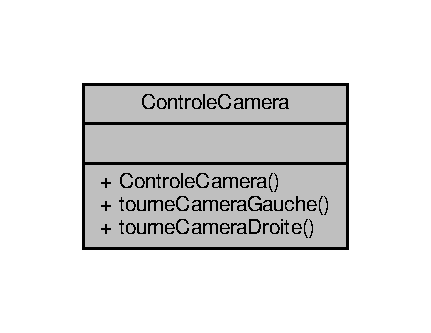
\includegraphics[width=207pt]{class_controle_camera__coll__graph}
\end{center}
\end{figure}
\subsubsection*{Connecteurs publics}
\begin{DoxyCompactItemize}
\item 
void \hyperlink{class_controle_camera_a119562aacbb4c0fbd4e5aa27a05ce7cc}{tourne\+Camera\+Gauche} (bool bouton\+Appuye)
\begin{DoxyCompactList}\small\item\em Permet de pivoter la caméra vers la gauche, en émettant la trame correspondante. Correspond à la croix directionnelle gauche de la manette. \end{DoxyCompactList}\item 
void \hyperlink{class_controle_camera_aac294c4e98a912199ba32d686e52f7ef}{tourne\+Camera\+Droite} (bool bouton\+Appuye)
\begin{DoxyCompactList}\small\item\em Permet de pivoter la caméra vers la droite, en émettant la trame correspondante. Correspond à la croix directionnelle droite de la manette. \end{DoxyCompactList}\end{DoxyCompactItemize}
\subsubsection*{Signaux}
\begin{DoxyCompactItemize}
\item 
void \hyperlink{class_controle_camera_ae6fda972cd90c8a14bc1c0171e1600e5}{trame\+Cree} (Q\+String trame)
\begin{DoxyCompactList}\small\item\em Signal émis lorsqu\textquotesingle{}une trame a été crée et prête à être transmise. \end{DoxyCompactList}\end{DoxyCompactItemize}
\subsubsection*{Fonctions membres publiques}
\begin{DoxyCompactItemize}
\item 
\hyperlink{class_controle_camera_afe5dd4f7158c6c18c78b52253fe78327}{Controle\+Camera} (Q\+Object $\ast$parent=nullptr)
\end{DoxyCompactItemize}


\subsubsection{Description détaillée}
\begin{DoxyAuthor}{Auteur}
Nicolas B\+O\+F\+F\+R\+E\+DO
\end{DoxyAuthor}
\begin{DoxyVersion}{Version}
1.\+1
\end{DoxyVersion}
\begin{DoxyDate}{Date}
Jeudi 13 Juin 2019 
\end{DoxyDate}


\subsubsection{Documentation des constructeurs et destructeur}
\mbox{\Hypertarget{class_controle_camera_afe5dd4f7158c6c18c78b52253fe78327}\label{class_controle_camera_afe5dd4f7158c6c18c78b52253fe78327}} 
\index{Controle\+Camera@{Controle\+Camera}!Controle\+Camera@{Controle\+Camera}}
\index{Controle\+Camera@{Controle\+Camera}!Controle\+Camera@{Controle\+Camera}}
\paragraph{\texorpdfstring{Controle\+Camera()}{ControleCamera()}}
{\footnotesize\ttfamily Controle\+Camera\+::\+Controle\+Camera (\begin{DoxyParamCaption}\item[{Q\+Object $\ast$}]{parent = {\ttfamily nullptr} }\end{DoxyParamCaption})\hspace{0.3cm}{\ttfamily [explicit]}}


\begin{DoxyCode}
00017                                               : QObject(parent)
00018 \{
00019 
00020 \}
\end{DoxyCode}


\subsubsection{Documentation des fonctions membres}
\mbox{\Hypertarget{class_controle_camera_aac294c4e98a912199ba32d686e52f7ef}\label{class_controle_camera_aac294c4e98a912199ba32d686e52f7ef}} 
\index{Controle\+Camera@{Controle\+Camera}!tourne\+Camera\+Droite@{tourne\+Camera\+Droite}}
\index{tourne\+Camera\+Droite@{tourne\+Camera\+Droite}!Controle\+Camera@{Controle\+Camera}}
\paragraph{\texorpdfstring{tourne\+Camera\+Droite}{tourneCameraDroite}}
{\footnotesize\ttfamily Controle\+Camera\+::tourne\+Camera\+Droite (\begin{DoxyParamCaption}\item[{bool}]{bouton\+Appuye }\end{DoxyParamCaption})\hspace{0.3cm}{\ttfamily [slot]}}


\begin{DoxyParams}{Paramètres}
{\em bouton\+Appuye} & bool vrai si le bouton est appuyé, faux sinon. \\
\hline
\end{DoxyParams}


Références \hyperlink{class_controle_camera_ae6fda972cd90c8a14bc1c0171e1600e5}{trame\+Cree()}.



Référencé par \hyperlink{class_controle_rov_acc4d5fea26770217df978d43df2ad51e}{Controle\+Rov\+::\+Controle\+Rov()}.


\begin{DoxyCode}
00039 \{
00040     QString trame = \textcolor{stringliteral}{"$TCA"} + QString::number(boutonAppuye) + \textcolor{stringliteral}{"\(\backslash\)n"};
00041     emit \hyperlink{class_controle_camera_ae6fda972cd90c8a14bc1c0171e1600e5}{trameCree}(trame);
00042 \}
\end{DoxyCode}
\mbox{\Hypertarget{class_controle_camera_a119562aacbb4c0fbd4e5aa27a05ce7cc}\label{class_controle_camera_a119562aacbb4c0fbd4e5aa27a05ce7cc}} 
\index{Controle\+Camera@{Controle\+Camera}!tourne\+Camera\+Gauche@{tourne\+Camera\+Gauche}}
\index{tourne\+Camera\+Gauche@{tourne\+Camera\+Gauche}!Controle\+Camera@{Controle\+Camera}}
\paragraph{\texorpdfstring{tourne\+Camera\+Gauche}{tourneCameraGauche}}
{\footnotesize\ttfamily Controle\+Camera\+::tourne\+Camera\+Gauche (\begin{DoxyParamCaption}\item[{bool}]{bouton\+Appuye }\end{DoxyParamCaption})\hspace{0.3cm}{\ttfamily [slot]}}


\begin{DoxyParams}{Paramètres}
{\em bouton\+Appuye} & bool vrai si le bouton est appuyé, faux sinon. \\
\hline
\end{DoxyParams}


Références \hyperlink{class_controle_camera_ae6fda972cd90c8a14bc1c0171e1600e5}{trame\+Cree()}.



Référencé par \hyperlink{class_controle_rov_acc4d5fea26770217df978d43df2ad51e}{Controle\+Rov\+::\+Controle\+Rov()}.


\begin{DoxyCode}
00028 \{
00029     QString trame = \textcolor{stringliteral}{"$TCA"} + QString::number(-boutonAppuye) + \textcolor{stringliteral}{"\(\backslash\)n"};
00030     emit \hyperlink{class_controle_camera_ae6fda972cd90c8a14bc1c0171e1600e5}{trameCree}(trame);
00031 \}
\end{DoxyCode}
\mbox{\Hypertarget{class_controle_camera_ae6fda972cd90c8a14bc1c0171e1600e5}\label{class_controle_camera_ae6fda972cd90c8a14bc1c0171e1600e5}} 
\index{Controle\+Camera@{Controle\+Camera}!trame\+Cree@{trame\+Cree}}
\index{trame\+Cree@{trame\+Cree}!Controle\+Camera@{Controle\+Camera}}
\paragraph{\texorpdfstring{trame\+Cree}{trameCree}}
{\footnotesize\ttfamily void Controle\+Camera\+::trame\+Cree (\begin{DoxyParamCaption}\item[{Q\+String}]{trame }\end{DoxyParamCaption})\hspace{0.3cm}{\ttfamily [signal]}}



Référencé par \hyperlink{class_controle_camera_aac294c4e98a912199ba32d686e52f7ef}{tourne\+Camera\+Droite()}, et \hyperlink{class_controle_camera_a119562aacbb4c0fbd4e5aa27a05ce7cc}{tourne\+Camera\+Gauche()}.



La documentation de cette classe a été générée à partir des fichiers suivants \+:\begin{DoxyCompactItemize}
\item 
\hyperlink{controlecamera_8h}{controlecamera.\+h}\item 
\hyperlink{controlecamera_8cpp}{controlecamera.\+cpp}\end{DoxyCompactItemize}

\hypertarget{class_controle_rov}{}\subsection{Référence de la classe Controle\+Rov}
\label{class_controle_rov}\index{Controle\+Rov@{Controle\+Rov}}


Déclaration de la classe \hyperlink{class_controle_rov}{Controle\+Rov}. Permet le contrôle des éléments du rov, en reliant la manette aux méthodes de déplacement.  




{\ttfamily \#include $<$controlerov.\+h$>$}



Graphe de collaboration de Controle\+Rov\+:
\nopagebreak
\begin{figure}[H]
\begin{center}
\leavevmode
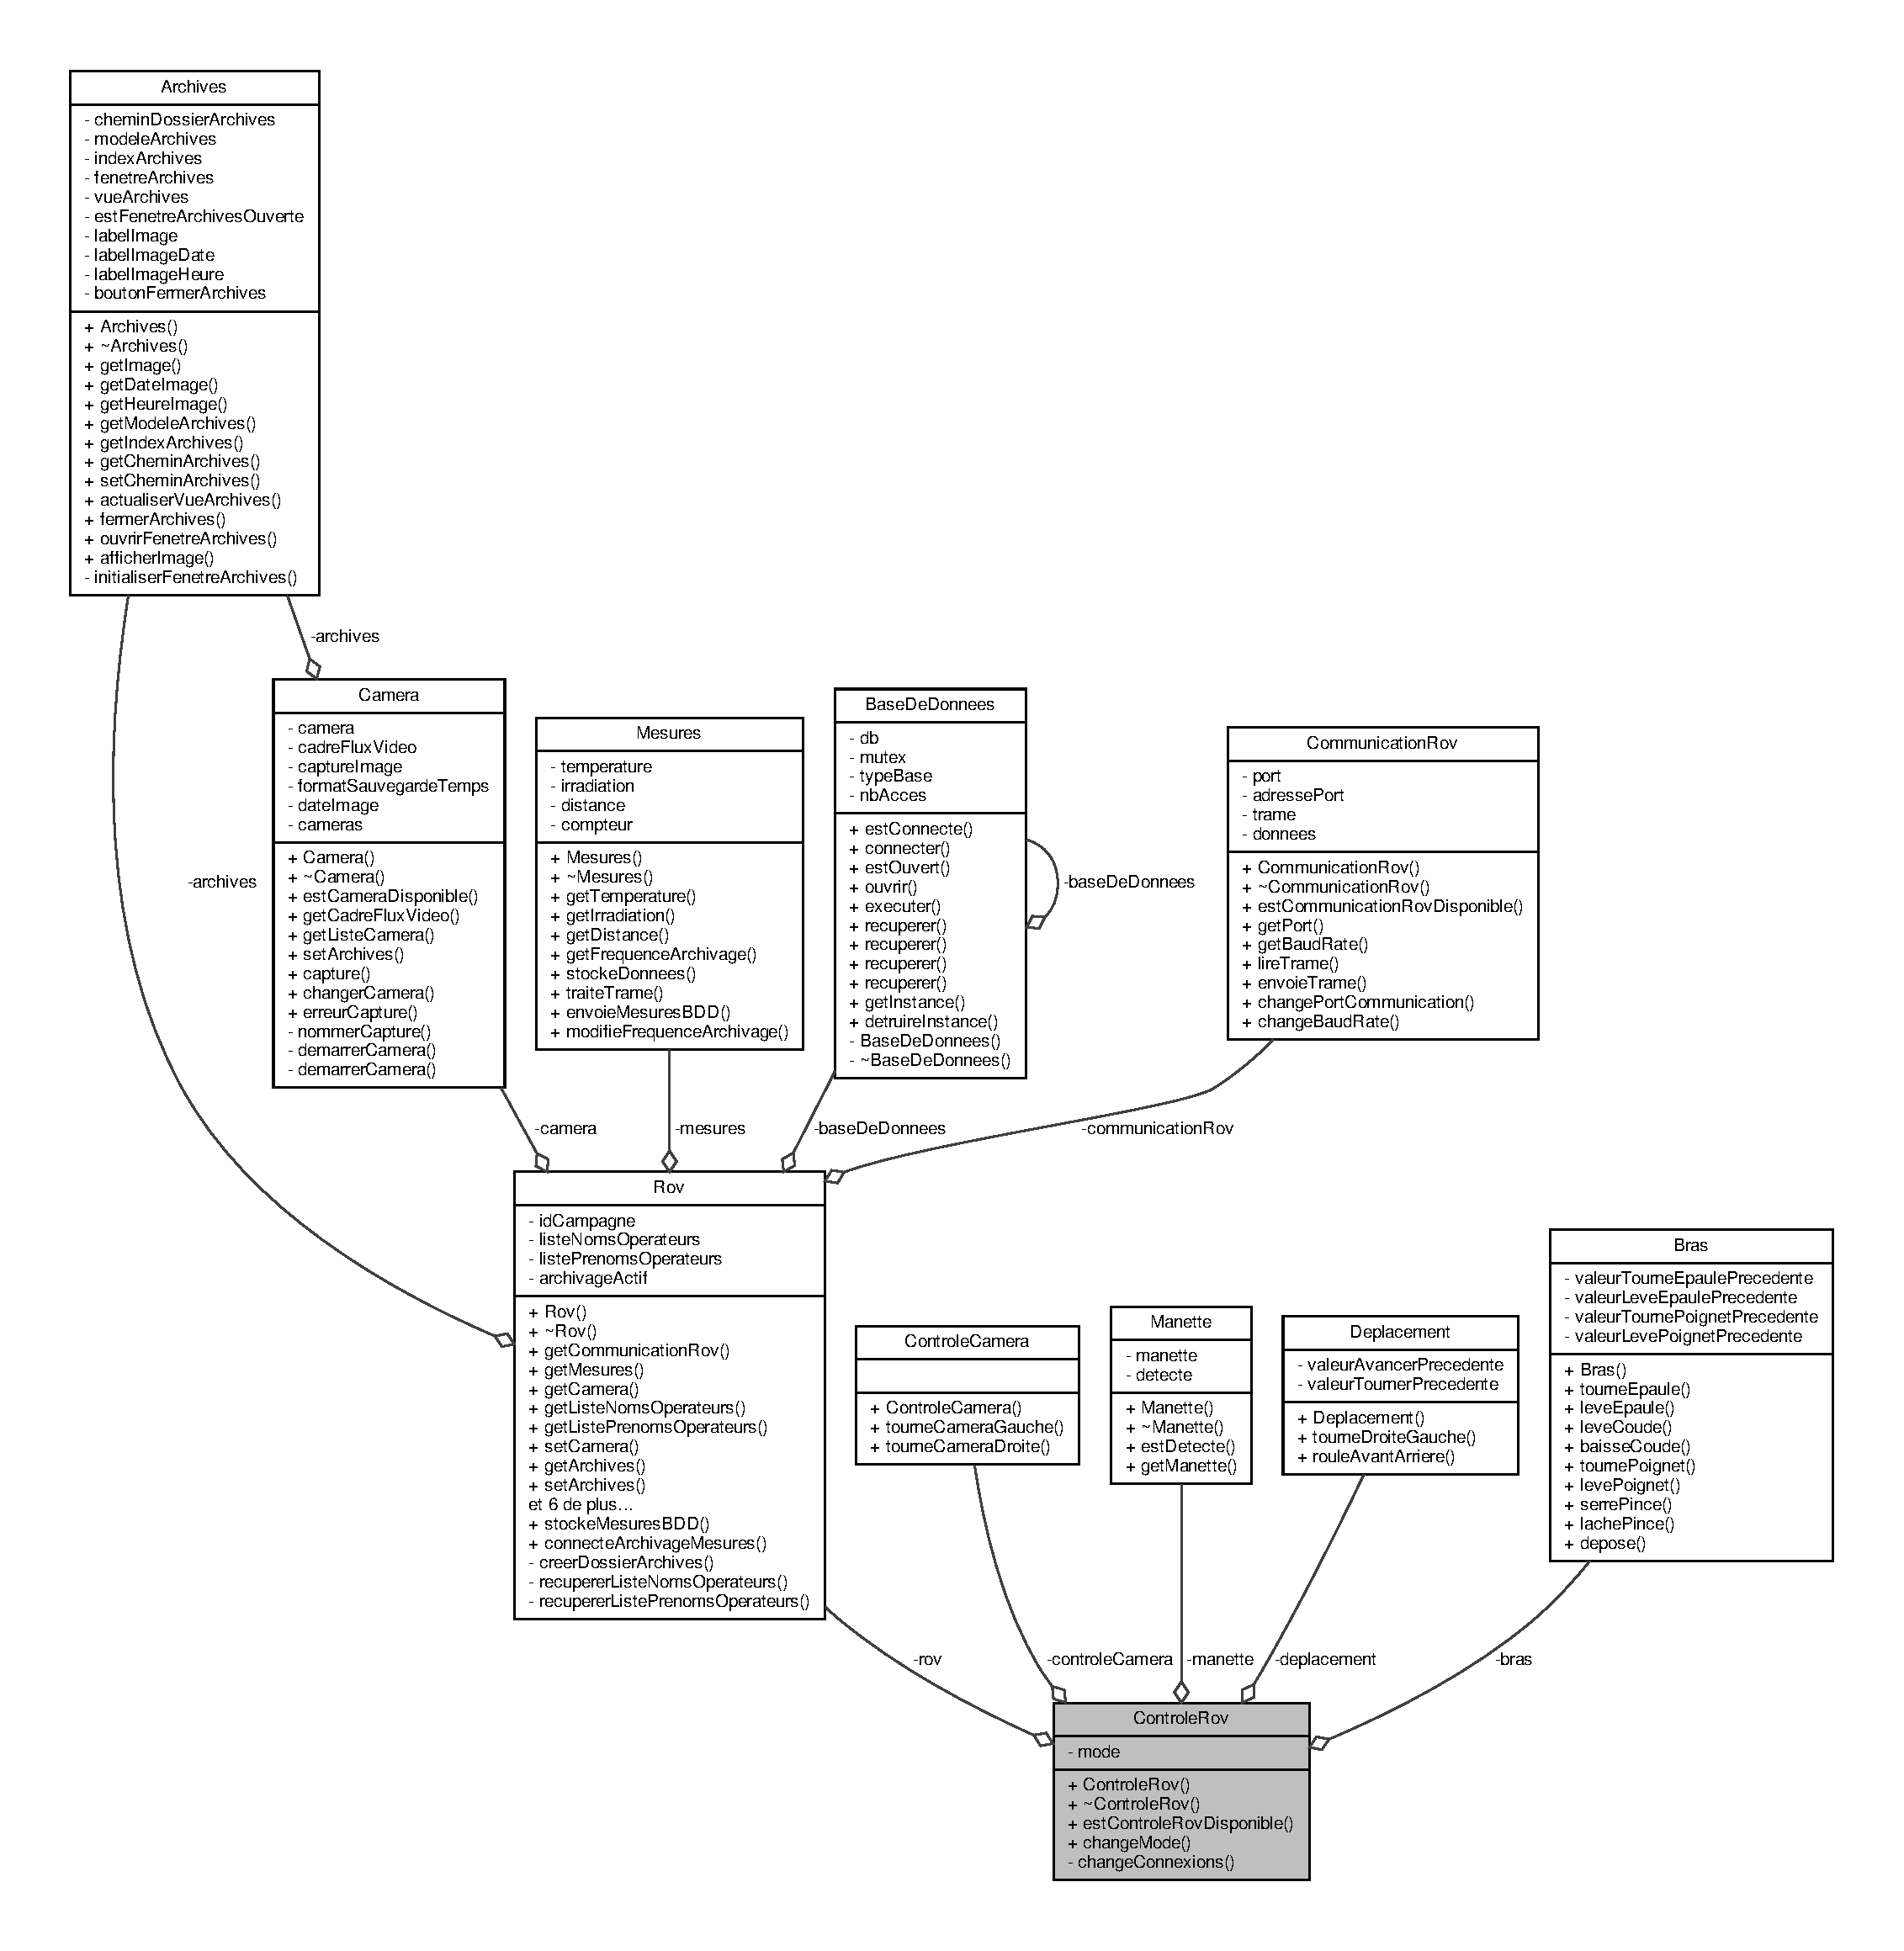
\includegraphics[width=350pt]{class_controle_rov__coll__graph}
\end{center}
\end{figure}
\subsubsection*{Connecteurs publics}
\begin{DoxyCompactItemize}
\item 
void \hyperlink{class_controle_rov_a206d52adf49b8510316b2885ea6b98b0}{change\+Mode} (bool appuye)
\begin{DoxyCompactList}\small\item\em change le mode de la manette (\hyperlink{class_deplacement}{Deplacement} / \hyperlink{class_bras}{Bras}). \end{DoxyCompactList}\end{DoxyCompactItemize}
\subsubsection*{Signaux}
\begin{DoxyCompactItemize}
\item 
void \hyperlink{class_controle_rov_a05506e1d8caf632b0394dcffd365c06f}{trame\+Cree} (Q\+String trame)
\begin{DoxyCompactList}\small\item\em Signal émis lorsqu\textquotesingle{}une trame a été crée et est destinée à l\textquotesingle{}envoi. \end{DoxyCompactList}\end{DoxyCompactItemize}
\subsubsection*{Fonctions membres publiques}
\begin{DoxyCompactItemize}
\item 
\hyperlink{class_controle_rov_acc4d5fea26770217df978d43df2ad51e}{Controle\+Rov} (Q\+Object $\ast$parent=nullptr, \hyperlink{class_rov}{Rov} $\ast$\hyperlink{class_controle_rov_a3620b701fbb3aebe6a57ca3f3f04c6ca}{rov}=nullptr)
\item 
\hyperlink{class_controle_rov_ab216ab83b9dfb738aa240c3846e65d39}{$\sim$\+Controle\+Rov} ()
\item 
bool \hyperlink{class_controle_rov_a9531520e50479fc2e339cd43f4c87066}{est\+Controle\+Rov\+Disponible} () const
\begin{DoxyCompactList}\small\item\em Renvoi l\textquotesingle{}état de connexion de la manette. \end{DoxyCompactList}\end{DoxyCompactItemize}
\subsubsection*{Fonctions membres privées}
\begin{DoxyCompactItemize}
\item 
void \hyperlink{class_controle_rov_a400d5766b9acabb45c1af5f8b22bbe47}{change\+Connexions} (int \hyperlink{class_controle_rov_a5d1fb6ad14da49e3c587199ae86dc28d}{mode})
\begin{DoxyCompactList}\small\item\em Permet de modifier les connexions entre la manette et les actions selon le mode de la manette. \end{DoxyCompactList}\end{DoxyCompactItemize}
\subsubsection*{Attributs privés}
\begin{DoxyCompactItemize}
\item 
\hyperlink{class_manette}{Manette} $\ast$ \hyperlink{class_controle_rov_af5caffd78d06f90d045b53ee87ad76df}{manette}
\begin{DoxyCompactList}\small\item\em manette utilisée \end{DoxyCompactList}\item 
\hyperlink{class_deplacement}{Deplacement} $\ast$ \hyperlink{class_controle_rov_ae96443be0a82814b27958e6ceb0a0acf}{deplacement}
\begin{DoxyCompactList}\small\item\em objet contenant les méthodes utilisées pour le déplacement du rov \end{DoxyCompactList}\item 
\hyperlink{class_bras}{Bras} $\ast$ \hyperlink{class_controle_rov_a1b2e394dd6332b2acd1be0770451e140}{bras}
\begin{DoxyCompactList}\small\item\em objet contenant les méthodes utilisées pour les mouvements du bras articulé \end{DoxyCompactList}\item 
\hyperlink{class_controle_camera}{Controle\+Camera} $\ast$ \hyperlink{class_controle_rov_ac88fe7f2367cca5a24aeda187ee0bac2}{controle\+Camera}
\begin{DoxyCompactList}\small\item\em objet contenant les méthodes utilisées pour les mouvements de la caméra \end{DoxyCompactList}\item 
\hyperlink{class_rov}{Rov} $\ast$ \hyperlink{class_controle_rov_a3620b701fbb3aebe6a57ca3f3f04c6ca}{rov}
\begin{DoxyCompactList}\small\item\em objet \hyperlink{class_rov}{Rov} contenant l\textquotesingle{}accès à la communication \end{DoxyCompactList}\item 
unsigned int \hyperlink{class_controle_rov_a5d1fb6ad14da49e3c587199ae86dc28d}{mode}
\begin{DoxyCompactList}\small\item\em Mode de la manette (0 pour déplacement, 1 pour bras) \end{DoxyCompactList}\end{DoxyCompactItemize}


\subsubsection{Description détaillée}
\begin{DoxyAuthor}{Auteur}
R\+E\+Y\+N\+I\+ER Jacques
\end{DoxyAuthor}
\begin{DoxyVersion}{Version}
1.\+1
\end{DoxyVersion}
\begin{DoxyDate}{Date}
Jeudi 13 Juin 2019 
\end{DoxyDate}


\subsubsection{Documentation des constructeurs et destructeur}
\mbox{\Hypertarget{class_controle_rov_acc4d5fea26770217df978d43df2ad51e}\label{class_controle_rov_acc4d5fea26770217df978d43df2ad51e}} 
\index{Controle\+Rov@{Controle\+Rov}!Controle\+Rov@{Controle\+Rov}}
\index{Controle\+Rov@{Controle\+Rov}!Controle\+Rov@{Controle\+Rov}}
\paragraph{\texorpdfstring{Controle\+Rov()}{ControleRov()}}
{\footnotesize\ttfamily Controle\+Rov\+::\+Controle\+Rov (\begin{DoxyParamCaption}\item[{Q\+Object $\ast$}]{parent = {\ttfamily nullptr},  }\item[{\hyperlink{class_rov}{Rov} $\ast$}]{rov = {\ttfamily nullptr} }\end{DoxyParamCaption})\hspace{0.3cm}{\ttfamily [explicit]}}



Références \hyperlink{class_controle_rov_a1b2e394dd6332b2acd1be0770451e140}{bras}, \hyperlink{class_controle_rov_a206d52adf49b8510316b2885ea6b98b0}{change\+Mode()}, \hyperlink{class_controle_rov_ac88fe7f2367cca5a24aeda187ee0bac2}{controle\+Camera}, \hyperlink{class_controle_rov_ae96443be0a82814b27958e6ceb0a0acf}{deplacement}, \hyperlink{class_communication_rov_ac243fcfb073f4ceaf58fab1d41207801}{Communication\+Rov\+::envoie\+Trame()}, \hyperlink{class_manette_a035c0a43a11e91889891b3c874f0a58d}{Manette\+::est\+Detecte()}, \hyperlink{class_rov_ad30543625f584e28bf785a80c59506dc}{Rov\+::get\+Communication\+Rov()}, \hyperlink{class_manette_a708eccb66e967e0fe575b19e9899ff5a}{Manette\+::get\+Manette()}, \hyperlink{class_controle_rov_af5caffd78d06f90d045b53ee87ad76df}{manette}, \hyperlink{class_deplacement_a65a1c6adfe5114d3cfefa631e0c91618}{Deplacement\+::roule\+Avant\+Arriere()}, \hyperlink{class_controle_camera_aac294c4e98a912199ba32d686e52f7ef}{Controle\+Camera\+::tourne\+Camera\+Droite()}, \hyperlink{class_controle_camera_a119562aacbb4c0fbd4e5aa27a05ce7cc}{Controle\+Camera\+::tourne\+Camera\+Gauche()}, \hyperlink{class_deplacement_a164cc606a6c5b8d55c1e5475d4d112e0}{Deplacement\+::tourne\+Droite\+Gauche()}, \hyperlink{class_deplacement_ae1a6d4a98304dee19d426ceeb6b7d5bb}{Deplacement\+::trame\+Cree()}, \hyperlink{class_controle_rov_a05506e1d8caf632b0394dcffd365c06f}{trame\+Cree()}, et \hyperlink{class_bras_ab442bf8d3e389c051b26b4b0741e7924}{Bras\+::trame\+Cree()}.


\begin{DoxyCode}
00021                                                   : QObject(parent), \hyperlink{class_controle_rov_a3620b701fbb3aebe6a57ca3f3f04c6ca}{rov}(rov), 
      \hyperlink{class_controle_rov_a5d1fb6ad14da49e3c587199ae86dc28d}{mode}(\hyperlink{controlerov_8h_a427f99e4fe2f812b0f49a09025623653}{MODE\_DEPLACEMENT})
00022 \{
00023     this->\hyperlink{class_controle_rov_a1b2e394dd6332b2acd1be0770451e140}{bras} = \textcolor{keyword}{new} \hyperlink{class_bras}{Bras}(\textcolor{keyword}{this});
00024     this->\hyperlink{class_controle_rov_ae96443be0a82814b27958e6ceb0a0acf}{deplacement} = \textcolor{keyword}{new} \hyperlink{class_deplacement}{Deplacement}(\textcolor{keyword}{this});
00025     this->\hyperlink{class_controle_rov_ac88fe7f2367cca5a24aeda187ee0bac2}{controleCamera} = \textcolor{keyword}{new} \hyperlink{class_controle_camera}{ControleCamera}(\textcolor{keyword}{this});
00026     this->\hyperlink{class_controle_rov_af5caffd78d06f90d045b53ee87ad76df}{manette} = \textcolor{keyword}{new} \hyperlink{class_manette}{Manette}(\textcolor{keyword}{this});
00027 
00028     \textcolor{keywordflow}{if}(\hyperlink{class_controle_rov_af5caffd78d06f90d045b53ee87ad76df}{manette}->\hyperlink{class_manette_a035c0a43a11e91889891b3c874f0a58d}{estDetecte}())
00029     \{
00030         connect(\hyperlink{class_controle_rov_af5caffd78d06f90d045b53ee87ad76df}{manette}->\hyperlink{class_manette_a708eccb66e967e0fe575b19e9899ff5a}{getManette}(), &QGamepad::axisLeftXChanged, 
      \hyperlink{class_controle_rov_ae96443be0a82814b27958e6ceb0a0acf}{deplacement}, &\hyperlink{class_deplacement_a164cc606a6c5b8d55c1e5475d4d112e0}{Deplacement::tourneDroiteGauche});
00031         connect(\hyperlink{class_controle_rov_af5caffd78d06f90d045b53ee87ad76df}{manette}->\hyperlink{class_manette_a708eccb66e967e0fe575b19e9899ff5a}{getManette}(), &QGamepad::axisLeftYChanged, 
      \hyperlink{class_controle_rov_ae96443be0a82814b27958e6ceb0a0acf}{deplacement}, &\hyperlink{class_deplacement_a65a1c6adfe5114d3cfefa631e0c91618}{Deplacement::rouleAvantArriere});
00032         connect(\hyperlink{class_controle_rov_af5caffd78d06f90d045b53ee87ad76df}{manette}->\hyperlink{class_manette_a708eccb66e967e0fe575b19e9899ff5a}{getManette}(), &QGamepad::buttonLeftChanged, 
      \hyperlink{class_controle_rov_ac88fe7f2367cca5a24aeda187ee0bac2}{controleCamera}, &\hyperlink{class_controle_camera_a119562aacbb4c0fbd4e5aa27a05ce7cc}{ControleCamera::tourneCameraGauche});
00033         connect(\hyperlink{class_controle_rov_af5caffd78d06f90d045b53ee87ad76df}{manette}->\hyperlink{class_manette_a708eccb66e967e0fe575b19e9899ff5a}{getManette}(), &QGamepad::buttonRightChanged, 
      \hyperlink{class_controle_rov_ac88fe7f2367cca5a24aeda187ee0bac2}{controleCamera}, &\hyperlink{class_controle_camera_aac294c4e98a912199ba32d686e52f7ef}{ControleCamera::tourneCameraDroite});
00034         connect(\hyperlink{class_controle_rov_af5caffd78d06f90d045b53ee87ad76df}{manette}->\hyperlink{class_manette_a708eccb66e967e0fe575b19e9899ff5a}{getManette}(), &QGamepad::buttonSelectChanged, \textcolor{keyword}{this}, &
      \hyperlink{class_controle_rov_a206d52adf49b8510316b2885ea6b98b0}{ControleRov::changeMode});
00035     \}
00036 
00037     \textcolor{comment}{// Connexion entre le signal émis d'une trame à envoyer au slot d'envoi de trame de la classe
       CommunicationRov.}
00038     connect(\hyperlink{class_controle_rov_a1b2e394dd6332b2acd1be0770451e140}{bras}, &\hyperlink{class_bras_ab442bf8d3e389c051b26b4b0741e7924}{Bras::trameCree}, this->rov->
      \hyperlink{class_rov_ad30543625f584e28bf785a80c59506dc}{getCommunicationRov}(), &\hyperlink{class_communication_rov_ac243fcfb073f4ceaf58fab1d41207801}{CommunicationRov::envoieTrame});
00039     \textcolor{comment}{// Connexion entre le signal émis d'une trame à envoyer au slot d'envoi de trame de la classe
       CommunicationRov.}
00040     connect(deplacement, &\hyperlink{class_deplacement_ae1a6d4a98304dee19d426ceeb6b7d5bb}{Deplacement::trameCree}, this->rov->
      \hyperlink{class_rov_ad30543625f584e28bf785a80c59506dc}{getCommunicationRov}(), &\hyperlink{class_communication_rov_ac243fcfb073f4ceaf58fab1d41207801}{CommunicationRov::envoieTrame});
00041 
00042     connect(\textcolor{keyword}{this}, &\hyperlink{class_controle_rov_a05506e1d8caf632b0394dcffd365c06f}{ControleRov::trameCree}, this->rov->
      \hyperlink{class_rov_ad30543625f584e28bf785a80c59506dc}{getCommunicationRov}(), &\hyperlink{class_communication_rov_ac243fcfb073f4ceaf58fab1d41207801}{CommunicationRov::envoieTrame});
00043 \}
\end{DoxyCode}
\mbox{\Hypertarget{class_controle_rov_ab216ab83b9dfb738aa240c3846e65d39}\label{class_controle_rov_ab216ab83b9dfb738aa240c3846e65d39}} 
\index{Controle\+Rov@{Controle\+Rov}!````~Controle\+Rov@{$\sim$\+Controle\+Rov}}
\index{````~Controle\+Rov@{$\sim$\+Controle\+Rov}!Controle\+Rov@{Controle\+Rov}}
\paragraph{\texorpdfstring{$\sim$\+Controle\+Rov()}{~ControleRov()}}
{\footnotesize\ttfamily Controle\+Rov\+::$\sim$\+Controle\+Rov (\begin{DoxyParamCaption}{ }\end{DoxyParamCaption})}


\begin{DoxyCode}
00046 \{
00047 \}
\end{DoxyCode}


\subsubsection{Documentation des fonctions membres}
\mbox{\Hypertarget{class_controle_rov_a400d5766b9acabb45c1af5f8b22bbe47}\label{class_controle_rov_a400d5766b9acabb45c1af5f8b22bbe47}} 
\index{Controle\+Rov@{Controle\+Rov}!change\+Connexions@{change\+Connexions}}
\index{change\+Connexions@{change\+Connexions}!Controle\+Rov@{Controle\+Rov}}
\paragraph{\texorpdfstring{change\+Connexions()}{changeConnexions()}}
{\footnotesize\ttfamily Controle\+Rov\+::change\+Connexions (\begin{DoxyParamCaption}\item[{int}]{mode }\end{DoxyParamCaption})\hspace{0.3cm}{\ttfamily [private]}}


\begin{DoxyParams}{Paramètres}
{\em mode} & int\\
\hline
{\em mode} & int Nouveau mode. \\
\hline
\end{DoxyParams}


Références \hyperlink{class_bras_a4b8e4791a454fcf884b1e7217a16a326}{Bras\+::baisse\+Coude()}, \hyperlink{class_controle_rov_a1b2e394dd6332b2acd1be0770451e140}{bras}, \hyperlink{class_controle_rov_ae96443be0a82814b27958e6ceb0a0acf}{deplacement}, \hyperlink{class_bras_a69d95616a74732e13b23bd90680d7d21}{Bras\+::depose()}, \hyperlink{class_manette_a708eccb66e967e0fe575b19e9899ff5a}{Manette\+::get\+Manette()}, \hyperlink{class_bras_a246e835f25bd61f0618c58aafea99ea1}{Bras\+::lache\+Pince()}, \hyperlink{class_bras_a197686a4ff55b4fe2384b2af44b8228b}{Bras\+::leve\+Coude()}, \hyperlink{class_bras_ac8f658db87d03bfbba6faa535326cc3a}{Bras\+::leve\+Epaule()}, \hyperlink{class_bras_ac95f54d8b02e7c88081f482fbbc40aef}{Bras\+::leve\+Poignet()}, \hyperlink{class_controle_rov_af5caffd78d06f90d045b53ee87ad76df}{manette}, \hyperlink{controlerov_8h_aa7e25e50c4dd52bfc6abcb3e450686d4}{M\+O\+D\+E\+\_\+\+B\+R\+AS}, \hyperlink{controlerov_8h_a427f99e4fe2f812b0f49a09025623653}{M\+O\+D\+E\+\_\+\+D\+E\+P\+L\+A\+C\+E\+M\+E\+NT}, \hyperlink{class_deplacement_a65a1c6adfe5114d3cfefa631e0c91618}{Deplacement\+::roule\+Avant\+Arriere()}, \hyperlink{class_bras_a55e143cf8e696ed214809ae25fb558d5}{Bras\+::serre\+Pince()}, \hyperlink{class_deplacement_a164cc606a6c5b8d55c1e5475d4d112e0}{Deplacement\+::tourne\+Droite\+Gauche()}, \hyperlink{class_bras_aaeacb18f22532a63559fc8430118169e}{Bras\+::tourne\+Epaule()}, et \hyperlink{class_bras_a15beae8aa104c2e689614486646ab402}{Bras\+::tourne\+Poignet()}.



Référencé par \hyperlink{class_controle_rov_a206d52adf49b8510316b2885ea6b98b0}{change\+Mode()}.


\begin{DoxyCode}
00093 \{
00094     \textcolor{keywordflow}{if} (\hyperlink{class_controle_rov_a5d1fb6ad14da49e3c587199ae86dc28d}{mode} == \hyperlink{controlerov_8h_aa7e25e50c4dd52bfc6abcb3e450686d4}{MODE\_BRAS})
00095     \{
00096         disconnect(\hyperlink{class_controle_rov_af5caffd78d06f90d045b53ee87ad76df}{manette}->\hyperlink{class_manette_a708eccb66e967e0fe575b19e9899ff5a}{getManette}(), &QGamepad::axisLeftXChanged, 
      \hyperlink{class_controle_rov_ae96443be0a82814b27958e6ceb0a0acf}{deplacement}, &\hyperlink{class_deplacement_a164cc606a6c5b8d55c1e5475d4d112e0}{Deplacement::tourneDroiteGauche});
00097         disconnect(\hyperlink{class_controle_rov_af5caffd78d06f90d045b53ee87ad76df}{manette}->\hyperlink{class_manette_a708eccb66e967e0fe575b19e9899ff5a}{getManette}(), &QGamepad::axisLeftYChanged, 
      \hyperlink{class_controle_rov_ae96443be0a82814b27958e6ceb0a0acf}{deplacement}, &\hyperlink{class_deplacement_a65a1c6adfe5114d3cfefa631e0c91618}{Deplacement::rouleAvantArriere});
00098 
00099         connect(\hyperlink{class_controle_rov_af5caffd78d06f90d045b53ee87ad76df}{manette}->\hyperlink{class_manette_a708eccb66e967e0fe575b19e9899ff5a}{getManette}(), &QGamepad::axisLeftXChanged, 
      \hyperlink{class_controle_rov_a1b2e394dd6332b2acd1be0770451e140}{bras}, &\hyperlink{class_bras_a15beae8aa104c2e689614486646ab402}{Bras::tournePoignet});
00100         connect(\hyperlink{class_controle_rov_af5caffd78d06f90d045b53ee87ad76df}{manette}->\hyperlink{class_manette_a708eccb66e967e0fe575b19e9899ff5a}{getManette}(), &QGamepad::axisLeftYChanged, 
      \hyperlink{class_controle_rov_a1b2e394dd6332b2acd1be0770451e140}{bras}, &\hyperlink{class_bras_ac95f54d8b02e7c88081f482fbbc40aef}{Bras::levePoignet});
00101 
00102         connect(\hyperlink{class_controle_rov_af5caffd78d06f90d045b53ee87ad76df}{manette}->\hyperlink{class_manette_a708eccb66e967e0fe575b19e9899ff5a}{getManette}(), &QGamepad::axisRightXChanged, 
      \hyperlink{class_controle_rov_a1b2e394dd6332b2acd1be0770451e140}{bras}, &\hyperlink{class_bras_aaeacb18f22532a63559fc8430118169e}{Bras::tourneEpaule});
00103         connect(\hyperlink{class_controle_rov_af5caffd78d06f90d045b53ee87ad76df}{manette}->\hyperlink{class_manette_a708eccb66e967e0fe575b19e9899ff5a}{getManette}(), &QGamepad::axisRightYChanged, 
      \hyperlink{class_controle_rov_a1b2e394dd6332b2acd1be0770451e140}{bras}, &\hyperlink{class_bras_ac8f658db87d03bfbba6faa535326cc3a}{Bras::leveEpaule});
00104 
00105         connect(\hyperlink{class_controle_rov_af5caffd78d06f90d045b53ee87ad76df}{manette}->\hyperlink{class_manette_a708eccb66e967e0fe575b19e9899ff5a}{getManette}(), &QGamepad::buttonUpChanged, 
      \hyperlink{class_controle_rov_a1b2e394dd6332b2acd1be0770451e140}{bras}, &\hyperlink{class_bras_a197686a4ff55b4fe2384b2af44b8228b}{Bras::leveCoude});
00106         connect(\hyperlink{class_controle_rov_af5caffd78d06f90d045b53ee87ad76df}{manette}->\hyperlink{class_manette_a708eccb66e967e0fe575b19e9899ff5a}{getManette}(), &QGamepad::buttonDownChanged, 
      \hyperlink{class_controle_rov_a1b2e394dd6332b2acd1be0770451e140}{bras}, &\hyperlink{class_bras_a4b8e4791a454fcf884b1e7217a16a326}{Bras::baisseCoude});
00107 
00108         connect(\hyperlink{class_controle_rov_af5caffd78d06f90d045b53ee87ad76df}{manette}->\hyperlink{class_manette_a708eccb66e967e0fe575b19e9899ff5a}{getManette}(), &QGamepad::buttonR1Changed, 
      \hyperlink{class_controle_rov_a1b2e394dd6332b2acd1be0770451e140}{bras}, &\hyperlink{class_bras_a55e143cf8e696ed214809ae25fb558d5}{Bras::serrePince});
00109         connect(\hyperlink{class_controle_rov_af5caffd78d06f90d045b53ee87ad76df}{manette}->\hyperlink{class_manette_a708eccb66e967e0fe575b19e9899ff5a}{getManette}(), &QGamepad::buttonL1Changed, 
      \hyperlink{class_controle_rov_a1b2e394dd6332b2acd1be0770451e140}{bras}, &\hyperlink{class_bras_a246e835f25bd61f0618c58aafea99ea1}{Bras::lachePince});
00110 
00111         connect(\hyperlink{class_controle_rov_af5caffd78d06f90d045b53ee87ad76df}{manette}->\hyperlink{class_manette_a708eccb66e967e0fe575b19e9899ff5a}{getManette}(), &QGamepad::buttonStartChanged, 
      \hyperlink{class_controle_rov_a1b2e394dd6332b2acd1be0770451e140}{bras}, &\hyperlink{class_bras_a69d95616a74732e13b23bd90680d7d21}{Bras::depose});
00112     \}
00113     \textcolor{keywordflow}{else} \textcolor{keywordflow}{if} (\hyperlink{class_controle_rov_a5d1fb6ad14da49e3c587199ae86dc28d}{mode} == \hyperlink{controlerov_8h_a427f99e4fe2f812b0f49a09025623653}{MODE\_DEPLACEMENT})
00114     \{
00115         disconnect(\hyperlink{class_controle_rov_af5caffd78d06f90d045b53ee87ad76df}{manette}->\hyperlink{class_manette_a708eccb66e967e0fe575b19e9899ff5a}{getManette}(), &QGamepad::axisLeftXChanged, 
      \hyperlink{class_controle_rov_a1b2e394dd6332b2acd1be0770451e140}{bras}, &\hyperlink{class_bras_a15beae8aa104c2e689614486646ab402}{Bras::tournePoignet});
00116         disconnect(\hyperlink{class_controle_rov_af5caffd78d06f90d045b53ee87ad76df}{manette}->\hyperlink{class_manette_a708eccb66e967e0fe575b19e9899ff5a}{getManette}(), &QGamepad::axisLeftYChanged, 
      \hyperlink{class_controle_rov_a1b2e394dd6332b2acd1be0770451e140}{bras}, &\hyperlink{class_bras_ac95f54d8b02e7c88081f482fbbc40aef}{Bras::levePoignet});
00117 
00118         disconnect(\hyperlink{class_controle_rov_af5caffd78d06f90d045b53ee87ad76df}{manette}->\hyperlink{class_manette_a708eccb66e967e0fe575b19e9899ff5a}{getManette}(), &QGamepad::axisRightXChanged, 
      \hyperlink{class_controle_rov_a1b2e394dd6332b2acd1be0770451e140}{bras}, &\hyperlink{class_bras_aaeacb18f22532a63559fc8430118169e}{Bras::tourneEpaule});
00119         disconnect(\hyperlink{class_controle_rov_af5caffd78d06f90d045b53ee87ad76df}{manette}->\hyperlink{class_manette_a708eccb66e967e0fe575b19e9899ff5a}{getManette}(), &QGamepad::axisRightYChanged, 
      \hyperlink{class_controle_rov_a1b2e394dd6332b2acd1be0770451e140}{bras}, &\hyperlink{class_bras_ac8f658db87d03bfbba6faa535326cc3a}{Bras::leveEpaule});
00120 
00121         disconnect(\hyperlink{class_controle_rov_af5caffd78d06f90d045b53ee87ad76df}{manette}->\hyperlink{class_manette_a708eccb66e967e0fe575b19e9899ff5a}{getManette}(), &QGamepad::buttonUpChanged, 
      \hyperlink{class_controle_rov_a1b2e394dd6332b2acd1be0770451e140}{bras}, &\hyperlink{class_bras_a197686a4ff55b4fe2384b2af44b8228b}{Bras::leveCoude});
00122         disconnect(\hyperlink{class_controle_rov_af5caffd78d06f90d045b53ee87ad76df}{manette}->\hyperlink{class_manette_a708eccb66e967e0fe575b19e9899ff5a}{getManette}(), &QGamepad::buttonDownChanged, 
      \hyperlink{class_controle_rov_a1b2e394dd6332b2acd1be0770451e140}{bras}, &\hyperlink{class_bras_a4b8e4791a454fcf884b1e7217a16a326}{Bras::baisseCoude});
00123 
00124         disconnect(\hyperlink{class_controle_rov_af5caffd78d06f90d045b53ee87ad76df}{manette}->\hyperlink{class_manette_a708eccb66e967e0fe575b19e9899ff5a}{getManette}(), &QGamepad::buttonR1Changed, 
      \hyperlink{class_controle_rov_a1b2e394dd6332b2acd1be0770451e140}{bras}, &\hyperlink{class_bras_a55e143cf8e696ed214809ae25fb558d5}{Bras::serrePince});
00125         disconnect(\hyperlink{class_controle_rov_af5caffd78d06f90d045b53ee87ad76df}{manette}->\hyperlink{class_manette_a708eccb66e967e0fe575b19e9899ff5a}{getManette}(), &QGamepad::buttonL1Changed, 
      \hyperlink{class_controle_rov_a1b2e394dd6332b2acd1be0770451e140}{bras}, &\hyperlink{class_bras_a246e835f25bd61f0618c58aafea99ea1}{Bras::lachePince});
00126 
00127         disconnect(\hyperlink{class_controle_rov_af5caffd78d06f90d045b53ee87ad76df}{manette}->\hyperlink{class_manette_a708eccb66e967e0fe575b19e9899ff5a}{getManette}(), &QGamepad::buttonStartChanged, 
      \hyperlink{class_controle_rov_a1b2e394dd6332b2acd1be0770451e140}{bras}, &\hyperlink{class_bras_a69d95616a74732e13b23bd90680d7d21}{Bras::depose});
00128 
00129         connect(\hyperlink{class_controle_rov_af5caffd78d06f90d045b53ee87ad76df}{manette}->\hyperlink{class_manette_a708eccb66e967e0fe575b19e9899ff5a}{getManette}(), &QGamepad::axisLeftXChanged, 
      \hyperlink{class_controle_rov_ae96443be0a82814b27958e6ceb0a0acf}{deplacement}, &\hyperlink{class_deplacement_a164cc606a6c5b8d55c1e5475d4d112e0}{Deplacement::tourneDroiteGauche});
00130         connect(\hyperlink{class_controle_rov_af5caffd78d06f90d045b53ee87ad76df}{manette}->\hyperlink{class_manette_a708eccb66e967e0fe575b19e9899ff5a}{getManette}(), &QGamepad::axisLeftYChanged, 
      \hyperlink{class_controle_rov_ae96443be0a82814b27958e6ceb0a0acf}{deplacement}, &\hyperlink{class_deplacement_a65a1c6adfe5114d3cfefa631e0c91618}{Deplacement::rouleAvantArriere});
00131     \}
00132     \textcolor{keywordflow}{else}
00133     \{
00134         qDebug() << Q\_FUNC\_INFO << \textcolor{stringliteral}{"ERREUR ! mode inconnu"};
00135     \}
00136 \}
\end{DoxyCode}
\mbox{\Hypertarget{class_controle_rov_a206d52adf49b8510316b2885ea6b98b0}\label{class_controle_rov_a206d52adf49b8510316b2885ea6b98b0}} 
\index{Controle\+Rov@{Controle\+Rov}!change\+Mode@{change\+Mode}}
\index{change\+Mode@{change\+Mode}!Controle\+Rov@{Controle\+Rov}}
\paragraph{\texorpdfstring{change\+Mode}{changeMode}}
{\footnotesize\ttfamily void Controle\+Rov\+::change\+Mode (\begin{DoxyParamCaption}\item[{bool}]{appuye }\end{DoxyParamCaption})\hspace{0.3cm}{\ttfamily [slot]}}

Permet de changer le mode de la manette, à la réception du signal d\textquotesingle{}appui de la touche Select. 

Références \hyperlink{class_controle_rov_a400d5766b9acabb45c1af5f8b22bbe47}{change\+Connexions()}, \hyperlink{class_controle_rov_a5d1fb6ad14da49e3c587199ae86dc28d}{mode}, \hyperlink{controlerov_8h_aa7e25e50c4dd52bfc6abcb3e450686d4}{M\+O\+D\+E\+\_\+\+B\+R\+AS}, \hyperlink{controlerov_8h_a427f99e4fe2f812b0f49a09025623653}{M\+O\+D\+E\+\_\+\+D\+E\+P\+L\+A\+C\+E\+M\+E\+NT}, et \hyperlink{class_controle_rov_a05506e1d8caf632b0394dcffd365c06f}{trame\+Cree()}.



Référencé par \hyperlink{class_controle_rov_acc4d5fea26770217df978d43df2ad51e}{Controle\+Rov()}.


\begin{DoxyCode}
00064 \{
00065     \textcolor{keywordflow}{if} (appuye == 1 && \hyperlink{class_controle_rov_a5d1fb6ad14da49e3c587199ae86dc28d}{mode} == \hyperlink{controlerov_8h_a427f99e4fe2f812b0f49a09025623653}{MODE\_DEPLACEMENT})
00066     \{
00067         qDebug() << Q\_FUNC\_INFO << \textcolor{stringliteral}{"Passage en mode Bras"};
00068         \hyperlink{class_controle_rov_a5d1fb6ad14da49e3c587199ae86dc28d}{mode} = \hyperlink{controlerov_8h_aa7e25e50c4dd52bfc6abcb3e450686d4}{MODE\_BRAS};
00069         emit \hyperlink{class_controle_rov_a05506e1d8caf632b0394dcffd365c06f}{trameCree}(\textcolor{stringliteral}{"$CBR1\(\backslash\)n"});
00070         \hyperlink{class_controle_rov_a400d5766b9acabb45c1af5f8b22bbe47}{changeConnexions}(\hyperlink{controlerov_8h_aa7e25e50c4dd52bfc6abcb3e450686d4}{MODE\_BRAS});
00071     \}
00072     \textcolor{keywordflow}{else} \textcolor{keywordflow}{if} (appuye == 1 && \hyperlink{class_controle_rov_a5d1fb6ad14da49e3c587199ae86dc28d}{mode} == \hyperlink{controlerov_8h_aa7e25e50c4dd52bfc6abcb3e450686d4}{MODE\_BRAS})
00073     \{
00074         qDebug() << Q\_FUNC\_INFO << \textcolor{stringliteral}{"Passage en mode Deplacement"};
00075         \hyperlink{class_controle_rov_a5d1fb6ad14da49e3c587199ae86dc28d}{mode} = \hyperlink{controlerov_8h_a427f99e4fe2f812b0f49a09025623653}{MODE\_DEPLACEMENT};
00076         emit \hyperlink{class_controle_rov_a05506e1d8caf632b0394dcffd365c06f}{trameCree}(\textcolor{stringliteral}{"$CRO1\(\backslash\)n"});
00077         \hyperlink{class_controle_rov_a400d5766b9acabb45c1af5f8b22bbe47}{changeConnexions}(\hyperlink{controlerov_8h_a427f99e4fe2f812b0f49a09025623653}{MODE\_DEPLACEMENT});
00078     \}
00079     \textcolor{keywordflow}{else} \textcolor{keywordflow}{if} (\hyperlink{class_controle_rov_a5d1fb6ad14da49e3c587199ae86dc28d}{mode} != \hyperlink{controlerov_8h_a427f99e4fe2f812b0f49a09025623653}{MODE\_DEPLACEMENT} && \hyperlink{class_controle_rov_a5d1fb6ad14da49e3c587199ae86dc28d}{mode} != 
      \hyperlink{controlerov_8h_aa7e25e50c4dd52bfc6abcb3e450686d4}{MODE\_BRAS})
00080     \{
00081         qDebug() << Q\_FUNC\_INFO << \textcolor{stringliteral}{"Erreur de mode ! Retour au mode de déplacement"};
00082         \hyperlink{class_controle_rov_a5d1fb6ad14da49e3c587199ae86dc28d}{mode} = \hyperlink{controlerov_8h_a427f99e4fe2f812b0f49a09025623653}{MODE\_DEPLACEMENT};
00083         \hyperlink{class_controle_rov_a400d5766b9acabb45c1af5f8b22bbe47}{changeConnexions}(\hyperlink{controlerov_8h_a427f99e4fe2f812b0f49a09025623653}{MODE\_DEPLACEMENT});
00084     \}
00085 \}
\end{DoxyCode}
\mbox{\Hypertarget{class_controle_rov_a9531520e50479fc2e339cd43f4c87066}\label{class_controle_rov_a9531520e50479fc2e339cd43f4c87066}} 
\index{Controle\+Rov@{Controle\+Rov}!est\+Controle\+Rov\+Disponible@{est\+Controle\+Rov\+Disponible}}
\index{est\+Controle\+Rov\+Disponible@{est\+Controle\+Rov\+Disponible}!Controle\+Rov@{Controle\+Rov}}
\paragraph{\texorpdfstring{est\+Controle\+Rov\+Disponible()}{estControleRovDisponible()}}
{\footnotesize\ttfamily Controle\+Rov\+::est\+Controle\+Rov\+Disponible (\begin{DoxyParamCaption}{ }\end{DoxyParamCaption}) const}

Indique si le \hyperlink{class_rov}{Rov} est contrôlable, ou non.

\begin{DoxyReturn}{Renvoie}
bool Etat de la manette (connectée, ou non). 
\end{DoxyReturn}


Références \hyperlink{class_manette_a035c0a43a11e91889891b3c874f0a58d}{Manette\+::est\+Detecte()}, et \hyperlink{class_controle_rov_af5caffd78d06f90d045b53ee87ad76df}{manette}.



Référencé par \hyperlink{class_i_h_m_rov_abbfcdc154a6ae7f941d186f6c90a5a2b}{I\+H\+M\+Rov\+::actualise\+Icones\+Etat()}.


\begin{DoxyCode}
00055 \{
00056     \textcolor{keywordflow}{return} \hyperlink{class_controle_rov_af5caffd78d06f90d045b53ee87ad76df}{manette}->\hyperlink{class_manette_a035c0a43a11e91889891b3c874f0a58d}{estDetecte}();
00057 \}
\end{DoxyCode}
\mbox{\Hypertarget{class_controle_rov_a05506e1d8caf632b0394dcffd365c06f}\label{class_controle_rov_a05506e1d8caf632b0394dcffd365c06f}} 
\index{Controle\+Rov@{Controle\+Rov}!trame\+Cree@{trame\+Cree}}
\index{trame\+Cree@{trame\+Cree}!Controle\+Rov@{Controle\+Rov}}
\paragraph{\texorpdfstring{trame\+Cree}{trameCree}}
{\footnotesize\ttfamily void Controle\+Rov\+::trame\+Cree (\begin{DoxyParamCaption}\item[{Q\+String}]{trame }\end{DoxyParamCaption})\hspace{0.3cm}{\ttfamily [signal]}}



Référencé par \hyperlink{class_controle_rov_a206d52adf49b8510316b2885ea6b98b0}{change\+Mode()}, et \hyperlink{class_controle_rov_acc4d5fea26770217df978d43df2ad51e}{Controle\+Rov()}.



\subsubsection{Documentation des données membres}
\mbox{\Hypertarget{class_controle_rov_a1b2e394dd6332b2acd1be0770451e140}\label{class_controle_rov_a1b2e394dd6332b2acd1be0770451e140}} 
\index{Controle\+Rov@{Controle\+Rov}!bras@{bras}}
\index{bras@{bras}!Controle\+Rov@{Controle\+Rov}}
\paragraph{\texorpdfstring{bras}{bras}}
{\footnotesize\ttfamily \hyperlink{class_bras}{Bras}$\ast$ Controle\+Rov\+::bras\hspace{0.3cm}{\ttfamily [private]}}



Référencé par \hyperlink{class_controle_rov_a400d5766b9acabb45c1af5f8b22bbe47}{change\+Connexions()}, et \hyperlink{class_controle_rov_acc4d5fea26770217df978d43df2ad51e}{Controle\+Rov()}.

\mbox{\Hypertarget{class_controle_rov_ac88fe7f2367cca5a24aeda187ee0bac2}\label{class_controle_rov_ac88fe7f2367cca5a24aeda187ee0bac2}} 
\index{Controle\+Rov@{Controle\+Rov}!controle\+Camera@{controle\+Camera}}
\index{controle\+Camera@{controle\+Camera}!Controle\+Rov@{Controle\+Rov}}
\paragraph{\texorpdfstring{controle\+Camera}{controleCamera}}
{\footnotesize\ttfamily \hyperlink{class_controle_camera}{Controle\+Camera}$\ast$ Controle\+Rov\+::controle\+Camera\hspace{0.3cm}{\ttfamily [private]}}



Référencé par \hyperlink{class_controle_rov_acc4d5fea26770217df978d43df2ad51e}{Controle\+Rov()}.

\mbox{\Hypertarget{class_controle_rov_ae96443be0a82814b27958e6ceb0a0acf}\label{class_controle_rov_ae96443be0a82814b27958e6ceb0a0acf}} 
\index{Controle\+Rov@{Controle\+Rov}!deplacement@{deplacement}}
\index{deplacement@{deplacement}!Controle\+Rov@{Controle\+Rov}}
\paragraph{\texorpdfstring{deplacement}{deplacement}}
{\footnotesize\ttfamily \hyperlink{class_deplacement}{Deplacement}$\ast$ Controle\+Rov\+::deplacement\hspace{0.3cm}{\ttfamily [private]}}



Référencé par \hyperlink{class_controle_rov_a400d5766b9acabb45c1af5f8b22bbe47}{change\+Connexions()}, et \hyperlink{class_controle_rov_acc4d5fea26770217df978d43df2ad51e}{Controle\+Rov()}.

\mbox{\Hypertarget{class_controle_rov_af5caffd78d06f90d045b53ee87ad76df}\label{class_controle_rov_af5caffd78d06f90d045b53ee87ad76df}} 
\index{Controle\+Rov@{Controle\+Rov}!manette@{manette}}
\index{manette@{manette}!Controle\+Rov@{Controle\+Rov}}
\paragraph{\texorpdfstring{manette}{manette}}
{\footnotesize\ttfamily \hyperlink{class_manette}{Manette}$\ast$ Controle\+Rov\+::manette\hspace{0.3cm}{\ttfamily [private]}}



Référencé par \hyperlink{class_controle_rov_a400d5766b9acabb45c1af5f8b22bbe47}{change\+Connexions()}, \hyperlink{class_controle_rov_acc4d5fea26770217df978d43df2ad51e}{Controle\+Rov()}, et \hyperlink{class_controle_rov_a9531520e50479fc2e339cd43f4c87066}{est\+Controle\+Rov\+Disponible()}.

\mbox{\Hypertarget{class_controle_rov_a5d1fb6ad14da49e3c587199ae86dc28d}\label{class_controle_rov_a5d1fb6ad14da49e3c587199ae86dc28d}} 
\index{Controle\+Rov@{Controle\+Rov}!mode@{mode}}
\index{mode@{mode}!Controle\+Rov@{Controle\+Rov}}
\paragraph{\texorpdfstring{mode}{mode}}
{\footnotesize\ttfamily unsigned int Controle\+Rov\+::mode\hspace{0.3cm}{\ttfamily [private]}}



Référencé par \hyperlink{class_controle_rov_a206d52adf49b8510316b2885ea6b98b0}{change\+Mode()}.

\mbox{\Hypertarget{class_controle_rov_a3620b701fbb3aebe6a57ca3f3f04c6ca}\label{class_controle_rov_a3620b701fbb3aebe6a57ca3f3f04c6ca}} 
\index{Controle\+Rov@{Controle\+Rov}!rov@{rov}}
\index{rov@{rov}!Controle\+Rov@{Controle\+Rov}}
\paragraph{\texorpdfstring{rov}{rov}}
{\footnotesize\ttfamily \hyperlink{class_rov}{Rov}$\ast$ Controle\+Rov\+::rov\hspace{0.3cm}{\ttfamily [private]}}



La documentation de cette classe a été générée à partir des fichiers suivants \+:\begin{DoxyCompactItemize}
\item 
\hyperlink{controlerov_8h}{controlerov.\+h}\item 
\hyperlink{controlerov_8cpp}{controlerov.\+cpp}\end{DoxyCompactItemize}

\hypertarget{class_deplacement}{}\subsection{Référence de la classe Deplacement}
\label{class_deplacement}\index{Deplacement@{Deplacement}}


Déclaration de la classe \hyperlink{class_deplacement}{Deplacement}. Réceptionne les signaux de la manette destiné aux déplacements du \hyperlink{class_rov}{Rov}, et émet les trames correspondantes.  




{\ttfamily \#include $<$deplacement.\+h$>$}



Graphe de collaboration de Deplacement\+:
\nopagebreak
\begin{figure}[H]
\begin{center}
\leavevmode
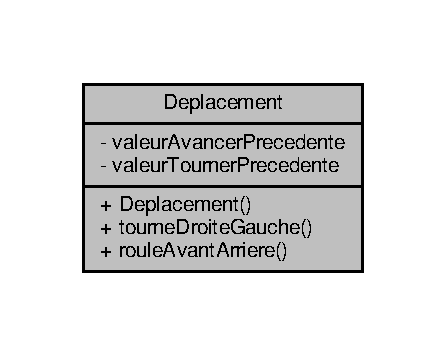
\includegraphics[width=214pt]{class_deplacement__coll__graph}
\end{center}
\end{figure}
\subsubsection*{Connecteurs publics}
\begin{DoxyCompactItemize}
\item 
void \hyperlink{class_deplacement_a164cc606a6c5b8d55c1e5475d4d112e0}{tourne\+Droite\+Gauche} (double valeur)
\begin{DoxyCompactList}\small\item\em Slot activé lorsque le joystick gauche est poussé à droite ou gauche. Emet un signal contenant la trame correspondante (déplacement \+: tourner à droite/gauche). \end{DoxyCompactList}\item 
void \hyperlink{class_deplacement_a65a1c6adfe5114d3cfefa631e0c91618}{roule\+Avant\+Arriere} (double valeur)
\begin{DoxyCompactList}\small\item\em Slot activé lorsque le joystick gauche est poussé en avant ou arrière. Emet un signal contenant la trame correspondante (déplacement \+: avancer/reculer). \end{DoxyCompactList}\end{DoxyCompactItemize}
\subsubsection*{Signaux}
\begin{DoxyCompactItemize}
\item 
void \hyperlink{class_deplacement_ae1a6d4a98304dee19d426ceeb6b7d5bb}{trame\+Cree} (Q\+String trame)
\begin{DoxyCompactList}\small\item\em Signal émis lorsqu\textquotesingle{}une trame est prête à être transmise. \end{DoxyCompactList}\end{DoxyCompactItemize}
\subsubsection*{Fonctions membres publiques}
\begin{DoxyCompactItemize}
\item 
\hyperlink{class_deplacement_a473f623358ffa95ac7385b49f128d23c}{Deplacement} (Q\+Object $\ast$parent=nullptr)
\end{DoxyCompactItemize}
\subsubsection*{Attributs privés}
\begin{DoxyCompactItemize}
\item 
Q\+String \hyperlink{class_deplacement_a419b8bb201dc4a4e927beed68923f8eb}{valeur\+Avancer\+Precedente}
\begin{DoxyCompactList}\small\item\em Dernière valeur de la trame Avancer émise. \end{DoxyCompactList}\item 
Q\+String \hyperlink{class_deplacement_a9d9b191747038f0f410626f38c4e75be}{valeur\+Tourner\+Precedente}
\begin{DoxyCompactList}\small\item\em Dernière valeur de la trame Tourner émise. \end{DoxyCompactList}\end{DoxyCompactItemize}


\subsubsection{Description détaillée}
\begin{DoxyAuthor}{Auteur}
R\+E\+Y\+N\+I\+ER Jacques
\end{DoxyAuthor}
\begin{DoxyVersion}{Version}
1.\+1
\end{DoxyVersion}
\begin{DoxyDate}{Date}
Jeudi 13 Juin 2019 
\end{DoxyDate}


\subsubsection{Documentation des constructeurs et destructeur}
\mbox{\Hypertarget{class_deplacement_a473f623358ffa95ac7385b49f128d23c}\label{class_deplacement_a473f623358ffa95ac7385b49f128d23c}} 
\index{Deplacement@{Deplacement}!Deplacement@{Deplacement}}
\index{Deplacement@{Deplacement}!Deplacement@{Deplacement}}
\paragraph{\texorpdfstring{Deplacement()}{Deplacement()}}
{\footnotesize\ttfamily Deplacement\+::\+Deplacement (\begin{DoxyParamCaption}\item[{Q\+Object $\ast$}]{parent = {\ttfamily nullptr} }\end{DoxyParamCaption})}


\begin{DoxyCode}
00018                                         : QObject(parent), 
      \hyperlink{class_deplacement_a419b8bb201dc4a4e927beed68923f8eb}{valeurAvancerPrecedente}(\textcolor{stringliteral}{"0"}), \hyperlink{class_deplacement_a9d9b191747038f0f410626f38c4e75be}{valeurTournerPrecedente}(\textcolor{stringliteral}{"0"})
00019 \{
00020 
00021 \}
\end{DoxyCode}


\subsubsection{Documentation des fonctions membres}
\mbox{\Hypertarget{class_deplacement_a65a1c6adfe5114d3cfefa631e0c91618}\label{class_deplacement_a65a1c6adfe5114d3cfefa631e0c91618}} 
\index{Deplacement@{Deplacement}!roule\+Avant\+Arriere@{roule\+Avant\+Arriere}}
\index{roule\+Avant\+Arriere@{roule\+Avant\+Arriere}!Deplacement@{Deplacement}}
\paragraph{\texorpdfstring{roule\+Avant\+Arriere}{rouleAvantArriere}}
{\footnotesize\ttfamily Deplacement\+::roule\+Avant\+Arriere (\begin{DoxyParamCaption}\item[{double}]{valeur }\end{DoxyParamCaption})\hspace{0.3cm}{\ttfamily [slot]}}

Emet la trame \+: avancer/reculer.


\begin{DoxyParams}{Paramètres}
{\em valeur} & double Force de l\textquotesingle{}appui sur le joystick (compris entre -\/1 et 1). \\
\hline
\end{DoxyParams}


Références \hyperlink{class_deplacement_ae1a6d4a98304dee19d426ceeb6b7d5bb}{trame\+Cree()}, et \hyperlink{class_deplacement_a419b8bb201dc4a4e927beed68923f8eb}{valeur\+Avancer\+Precedente}.



Référencé par \hyperlink{class_controle_rov_a400d5766b9acabb45c1af5f8b22bbe47}{Controle\+Rov\+::change\+Connexions()}, et \hyperlink{class_controle_rov_acc4d5fea26770217df978d43df2ad51e}{Controle\+Rov\+::\+Controle\+Rov()}.


\begin{DoxyCode}
00055 \{
00056     QString trame = \textcolor{stringliteral}{""};
00057     valeur = round(valeur * 3);
00058 
00059     \textcolor{keywordflow}{if}(valeur > 0)
00060         trame = \textcolor{stringliteral}{"$RRO"} + QString::number(-valeur) + \textcolor{stringliteral}{"\(\backslash\)n"};
00061     \textcolor{keywordflow}{else} \textcolor{keywordflow}{if}(valeur < 0)
00062         trame = \textcolor{stringliteral}{"$ARO"} + QString::number(-valeur) + \textcolor{stringliteral}{"\(\backslash\)n"};
00063     \textcolor{keywordflow}{else}
00064         trame = \textcolor{stringliteral}{"$ARO0\(\backslash\)n"};
00065 
00066     \textcolor{keywordflow}{if} (QString::number(valeur) != \hyperlink{class_deplacement_a419b8bb201dc4a4e927beed68923f8eb}{valeurAvancerPrecedente})
00067     \{
00068         emit \hyperlink{class_deplacement_ae1a6d4a98304dee19d426ceeb6b7d5bb}{trameCree}(trame);
00069         \hyperlink{class_deplacement_a419b8bb201dc4a4e927beed68923f8eb}{valeurAvancerPrecedente} = QString::number(valeur);
00070     \}
00071 \}
\end{DoxyCode}
\mbox{\Hypertarget{class_deplacement_a164cc606a6c5b8d55c1e5475d4d112e0}\label{class_deplacement_a164cc606a6c5b8d55c1e5475d4d112e0}} 
\index{Deplacement@{Deplacement}!tourne\+Droite\+Gauche@{tourne\+Droite\+Gauche}}
\index{tourne\+Droite\+Gauche@{tourne\+Droite\+Gauche}!Deplacement@{Deplacement}}
\paragraph{\texorpdfstring{tourne\+Droite\+Gauche}{tourneDroiteGauche}}
{\footnotesize\ttfamily Deplacement\+::tourne\+Droite\+Gauche (\begin{DoxyParamCaption}\item[{double}]{valeur }\end{DoxyParamCaption})\hspace{0.3cm}{\ttfamily [slot]}}

Emet la trame \+: tourner à droite/gauche.


\begin{DoxyParams}{Paramètres}
{\em valeur} & double Force de l\textquotesingle{}appui sur le joystick (compris entre -\/1 et 1). \\
\hline
\end{DoxyParams}


Références \hyperlink{class_deplacement_ae1a6d4a98304dee19d426ceeb6b7d5bb}{trame\+Cree()}, et \hyperlink{class_deplacement_a9d9b191747038f0f410626f38c4e75be}{valeur\+Tourner\+Precedente}.



Référencé par \hyperlink{class_controle_rov_a400d5766b9acabb45c1af5f8b22bbe47}{Controle\+Rov\+::change\+Connexions()}, et \hyperlink{class_controle_rov_acc4d5fea26770217df978d43df2ad51e}{Controle\+Rov\+::\+Controle\+Rov()}.


\begin{DoxyCode}
00030 \{
00031     QString trame = \textcolor{stringliteral}{""};
00032 
00033     valeur = round(valeur);
00034 
00035     \textcolor{keywordflow}{if}(valeur > 0)
00036         trame = \textcolor{stringliteral}{"$DRO"} + QString::number(valeur) + \textcolor{stringliteral}{"\(\backslash\)n"};
00037     \textcolor{keywordflow}{else} \textcolor{keywordflow}{if}(valeur < 0)
00038         trame = \textcolor{stringliteral}{"$GRO"} + QString::number(-valeur) + \textcolor{stringliteral}{"\(\backslash\)n"};
00039     \textcolor{keywordflow}{else}
00040         trame = \textcolor{stringliteral}{"$DRO0\(\backslash\)n"};
00041 
00042     \textcolor{keywordflow}{if} (QString::number(valeur) != \hyperlink{class_deplacement_a9d9b191747038f0f410626f38c4e75be}{valeurTournerPrecedente})
00043     \{
00044         emit \hyperlink{class_deplacement_ae1a6d4a98304dee19d426ceeb6b7d5bb}{trameCree}(trame);
00045         \hyperlink{class_deplacement_a9d9b191747038f0f410626f38c4e75be}{valeurTournerPrecedente} = QString::number(valeur);
00046     \}
00047 \}
\end{DoxyCode}
\mbox{\Hypertarget{class_deplacement_ae1a6d4a98304dee19d426ceeb6b7d5bb}\label{class_deplacement_ae1a6d4a98304dee19d426ceeb6b7d5bb}} 
\index{Deplacement@{Deplacement}!trame\+Cree@{trame\+Cree}}
\index{trame\+Cree@{trame\+Cree}!Deplacement@{Deplacement}}
\paragraph{\texorpdfstring{trame\+Cree}{trameCree}}
{\footnotesize\ttfamily void Deplacement\+::trame\+Cree (\begin{DoxyParamCaption}\item[{Q\+String}]{trame }\end{DoxyParamCaption})\hspace{0.3cm}{\ttfamily [signal]}}


\begin{DoxyParams}{Paramètres}
{\em trame} & Q\+String Trame à transmettre. \\
\hline
\end{DoxyParams}


Référencé par \hyperlink{class_controle_rov_acc4d5fea26770217df978d43df2ad51e}{Controle\+Rov\+::\+Controle\+Rov()}, \hyperlink{class_deplacement_a65a1c6adfe5114d3cfefa631e0c91618}{roule\+Avant\+Arriere()}, et \hyperlink{class_deplacement_a164cc606a6c5b8d55c1e5475d4d112e0}{tourne\+Droite\+Gauche()}.



\subsubsection{Documentation des données membres}
\mbox{\Hypertarget{class_deplacement_a419b8bb201dc4a4e927beed68923f8eb}\label{class_deplacement_a419b8bb201dc4a4e927beed68923f8eb}} 
\index{Deplacement@{Deplacement}!valeur\+Avancer\+Precedente@{valeur\+Avancer\+Precedente}}
\index{valeur\+Avancer\+Precedente@{valeur\+Avancer\+Precedente}!Deplacement@{Deplacement}}
\paragraph{\texorpdfstring{valeur\+Avancer\+Precedente}{valeurAvancerPrecedente}}
{\footnotesize\ttfamily Q\+String Deplacement\+::valeur\+Avancer\+Precedente\hspace{0.3cm}{\ttfamily [private]}}



Référencé par \hyperlink{class_deplacement_a65a1c6adfe5114d3cfefa631e0c91618}{roule\+Avant\+Arriere()}.

\mbox{\Hypertarget{class_deplacement_a9d9b191747038f0f410626f38c4e75be}\label{class_deplacement_a9d9b191747038f0f410626f38c4e75be}} 
\index{Deplacement@{Deplacement}!valeur\+Tourner\+Precedente@{valeur\+Tourner\+Precedente}}
\index{valeur\+Tourner\+Precedente@{valeur\+Tourner\+Precedente}!Deplacement@{Deplacement}}
\paragraph{\texorpdfstring{valeur\+Tourner\+Precedente}{valeurTournerPrecedente}}
{\footnotesize\ttfamily Q\+String Deplacement\+::valeur\+Tourner\+Precedente\hspace{0.3cm}{\ttfamily [private]}}



Référencé par \hyperlink{class_deplacement_a164cc606a6c5b8d55c1e5475d4d112e0}{tourne\+Droite\+Gauche()}.



La documentation de cette classe a été générée à partir des fichiers suivants \+:\begin{DoxyCompactItemize}
\item 
\hyperlink{deplacement_8h}{deplacement.\+h}\item 
\hyperlink{deplacement_8cpp}{deplacement.\+cpp}\end{DoxyCompactItemize}

\hypertarget{class_i_h_m_rov}{}\subsection{Référence de la classe I\+H\+M\+Rov}
\label{class_i_h_m_rov}\index{I\+H\+M\+Rov@{I\+H\+M\+Rov}}


Déclaration de la classe \hyperlink{class_rov}{Rov}.  




{\ttfamily \#include $<$ihmrov.\+h$>$}



Graphe de collaboration de I\+H\+M\+Rov\+:
\nopagebreak
\begin{figure}[H]
\begin{center}
\leavevmode
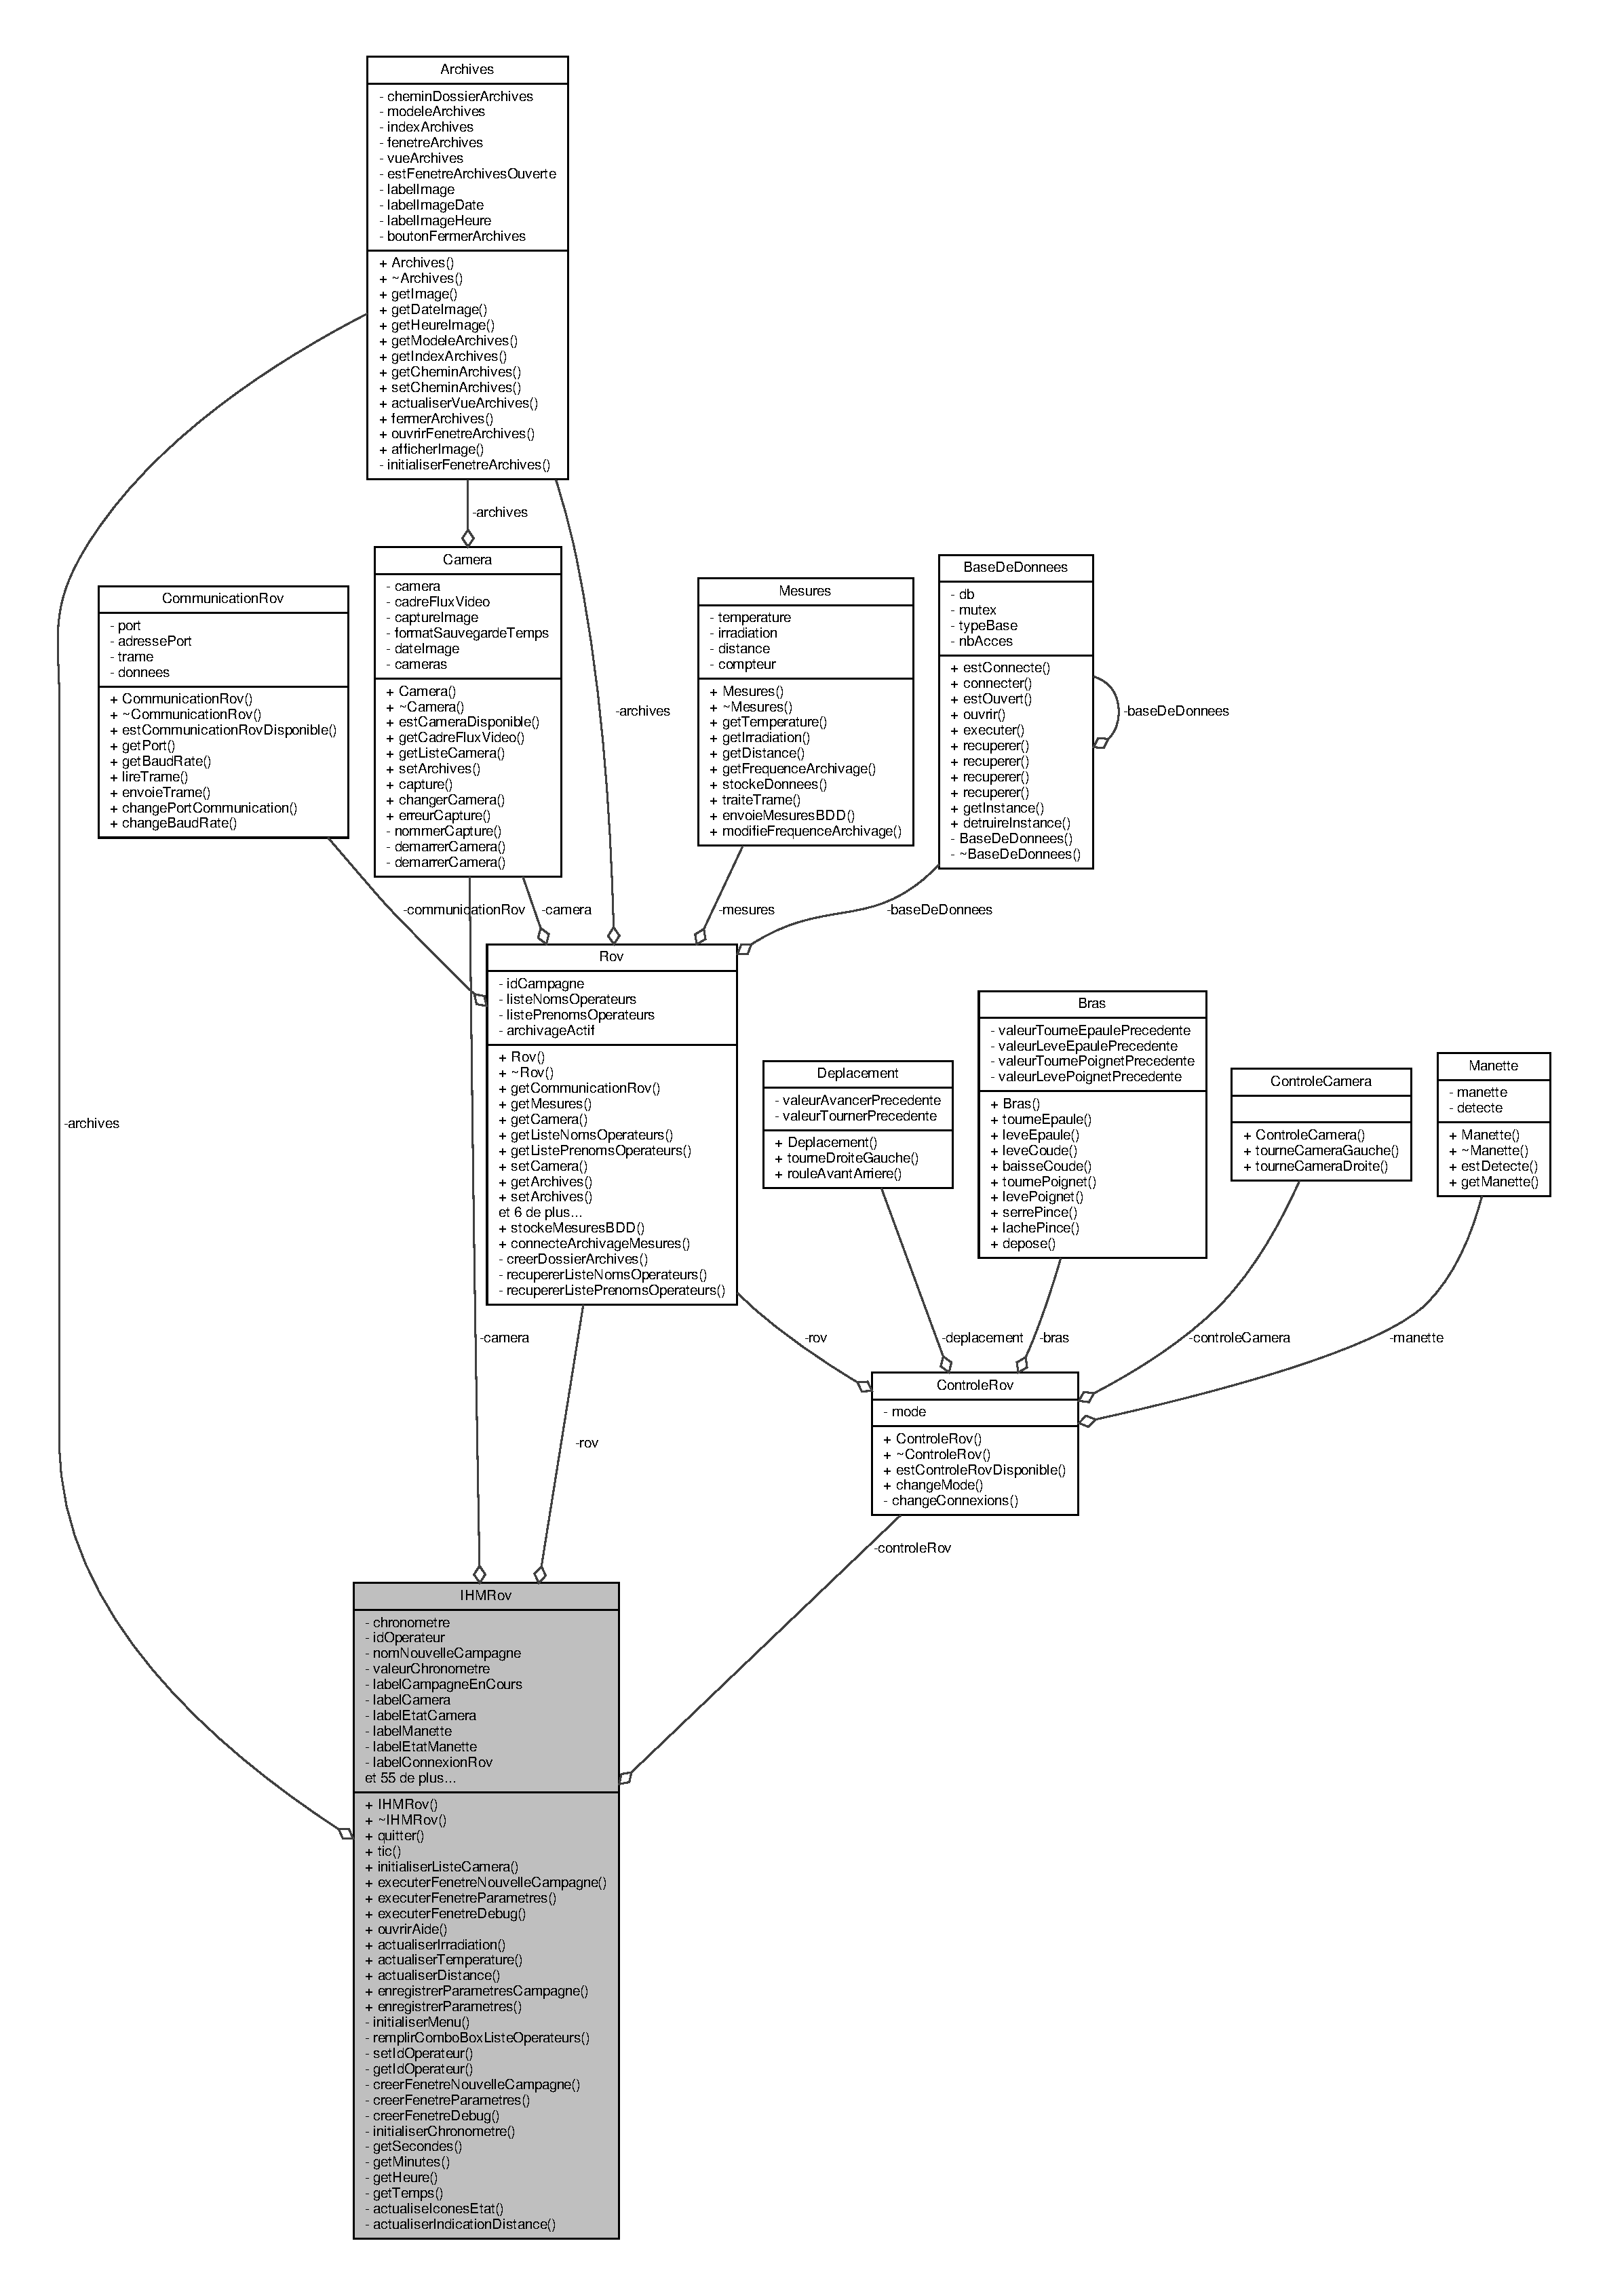
\includegraphics[width=350pt]{class_i_h_m_rov__coll__graph}
\end{center}
\end{figure}
\subsubsection*{Connecteurs publics}
\begin{DoxyCompactItemize}
\item 
void \hyperlink{class_i_h_m_rov_a6446087033d8ead72d16451b4a29c44e}{quitter} ()
\begin{DoxyCompactList}\small\item\em Permet de fermer l\textquotesingle{}application. \end{DoxyCompactList}\item 
void \hyperlink{class_i_h_m_rov_a4a0d3a0741d0669ede732b630eae54c6}{tic} ()
\begin{DoxyCompactList}\small\item\em Actualise l\textquotesingle{}affichage du temps chaque seconde et actualise l\textquotesingle{}état des icones de rov, manette, et camera. \end{DoxyCompactList}\item 
void \hyperlink{class_i_h_m_rov_af3e46f174ab2fdeaebb2d00e6b8bcb33}{initialiser\+Liste\+Camera} ()
\begin{DoxyCompactList}\small\item\em Ajoute les caméras détectées dans une liste déroulante. \end{DoxyCompactList}\item 
void \hyperlink{class_i_h_m_rov_a3169e8cd9132ece69af974648066c6c1}{executer\+Fenetre\+Nouvelle\+Campagne} ()
\begin{DoxyCompactList}\small\item\em Slot permettant de creer une nouvelle campagne. \end{DoxyCompactList}\item 
void \hyperlink{class_i_h_m_rov_a2ec97de9b75c073c6a4dd0792a284002}{executer\+Fenetre\+Parametres} ()
\begin{DoxyCompactList}\small\item\em Affiche la fenêtre Paramètres. \end{DoxyCompactList}\item 
void \hyperlink{class_i_h_m_rov_a8931cade7a1613975da7174b5c2e84d2}{executer\+Fenetre\+Debug} ()
\begin{DoxyCompactList}\small\item\em Affiche la fenêtre de Debug. \end{DoxyCompactList}\item 
void \hyperlink{class_i_h_m_rov_a45a10161fde8c6373918ec30f16a8b5e}{ouvrir\+Aide} ()
\begin{DoxyCompactList}\small\item\em ouvrir une fenetre informative sur l\textquotesingle{}application. \end{DoxyCompactList}\item 
void \hyperlink{class_i_h_m_rov_a9a5108ce8f73fad9a38d02881ec5ae62}{actualiser\+Irradiation} (double irradiation)
\begin{DoxyCompactList}\small\item\em Permet d\textquotesingle{}actualiser l\textquotesingle{}affichage de l\textquotesingle{}irradiation sur l\textquotesingle{}I\+HM. \end{DoxyCompactList}\item 
void \hyperlink{class_i_h_m_rov_ae5f2c89b06d7dc09e9974428b14799f1}{actualiser\+Temperature} (double temperature)
\begin{DoxyCompactList}\small\item\em Permet d\textquotesingle{}actualiser l\textquotesingle{}affichage de la temperature sur l\textquotesingle{}I\+HM. \end{DoxyCompactList}\item 
void \hyperlink{class_i_h_m_rov_a891d51cf532d9cc8fc56c63a0c61e663}{actualiser\+Distance} (double distance)
\begin{DoxyCompactList}\small\item\em Permet d\textquotesingle{}actualiser l\textquotesingle{}affichage de la distance sur l\textquotesingle{}I\+HM. \end{DoxyCompactList}\item 
void \hyperlink{class_i_h_m_rov_a229194814bfb1fc94ab3cc86d6411921}{enregistrer\+Parametres\+Campagne} ()
\begin{DoxyCompactList}\small\item\em Methode émettant l\textquotesingle{}ordre d\textquotesingle{}enregistrer les paramètres des la campagne. \end{DoxyCompactList}\item 
void \hyperlink{class_i_h_m_rov_a94d31f4e748f3e4549eab42c8bc7e367}{enregistrer\+Parametres} ()
\begin{DoxyCompactList}\small\item\em Applique les paramètres choisis par l\textquotesingle{}utilisateur suite à la fenêtre Paramètres. \end{DoxyCompactList}\end{DoxyCompactItemize}
\subsubsection*{Signaux}
\begin{DoxyCompactItemize}
\item 
void \hyperlink{class_i_h_m_rov_a4a4a90ab6d074aa54466f3f87db2f81c}{creation\+Campagne} ()
\item 
void \hyperlink{class_i_h_m_rov_afcfb7f60c126fbaa87cb3f501189cc39}{nouvelle\+Frequence\+Archivage} (int)
\item 
void \hyperlink{class_i_h_m_rov_ae64280b18ebe069c1f64bd5f19ef3a2e}{nouveau\+Port\+Com} (Q\+String)
\item 
void \hyperlink{class_i_h_m_rov_a051d1d8d545e97c6b838df9054dddc6f}{nouveau\+Baud\+Rate} (Q\+String)
\item 
void \hyperlink{class_i_h_m_rov_accf04daf204c5810c8a6099bb7e37b7e}{parametres\+Sauvegardes} ()
\end{DoxyCompactItemize}
\subsubsection*{Fonctions membres publiques}
\begin{DoxyCompactItemize}
\item 
\hyperlink{class_i_h_m_rov_a5dac1fb4612866cc61f699a415e0ef6b}{I\+H\+M\+Rov} (Q\+Widget $\ast$parent=nullptr)
\begin{DoxyCompactList}\small\item\em Constructeur de la classe \hyperlink{class_i_h_m_rov}{I\+H\+M\+Rov}. \end{DoxyCompactList}\item 
\hyperlink{class_i_h_m_rov_ab861463889934a3b6083b7a29c6adf45}{$\sim$\+I\+H\+M\+Rov} ()
\begin{DoxyCompactList}\small\item\em Destructeur de la classe \hyperlink{class_i_h_m_rov}{I\+H\+M\+Rov}. \end{DoxyCompactList}\end{DoxyCompactItemize}
\subsubsection*{Fonctions membres privées}
\begin{DoxyCompactItemize}
\item 
void \hyperlink{class_i_h_m_rov_aebbcb2325c2d1a88a012d8408e2d6223}{initialiser\+Menu} ()
\begin{DoxyCompactList}\small\item\em initialise la barre de menu \end{DoxyCompactList}\item 
void \hyperlink{class_i_h_m_rov_a752a8dc2b3b68d536e94ff8bfb62f46f}{remplir\+Combo\+Box\+Liste\+Operateurs} ()
\begin{DoxyCompactList}\small\item\em Méthode permettant de remplir le Combo\+Box de la liste des opérateurs au démarrage de l\textquotesingle{}I\+HM. \end{DoxyCompactList}\item 
void \hyperlink{class_i_h_m_rov_a021be212b27d0c4a08e14695521aacbc}{set\+Id\+Operateur} (int \hyperlink{class_i_h_m_rov_a110af5c174e9fbba12bffbe0301ed690}{id\+Operateur})
\begin{DoxyCompactList}\small\item\em Mutateur de l\textquotesingle{}attribut id\+Operateur. \end{DoxyCompactList}\item 
int \hyperlink{class_i_h_m_rov_a79cddc1e905195eb11a8960abadf7d2f}{get\+Id\+Operateur} ()
\begin{DoxyCompactList}\small\item\em Accesseur de l\textquotesingle{}attribut id\+Operateur. \end{DoxyCompactList}\item 
void \hyperlink{class_i_h_m_rov_a08bf623a890df272f738c1ff8631213f}{creer\+Fenetre\+Nouvelle\+Campagne} ()
\begin{DoxyCompactList}\small\item\em Méthode permettant d\textquotesingle{}initialiser la fenetre de création d\textquotesingle{}une nouvelle campagne. \end{DoxyCompactList}\item 
void \hyperlink{class_i_h_m_rov_aed451139ac09ef18b7c92637761d80ce}{creer\+Fenetre\+Parametres} ()
\begin{DoxyCompactList}\small\item\em Crée la fenêtre de Paramètres. \end{DoxyCompactList}\item 
void \hyperlink{class_i_h_m_rov_a30b49bada719a73e0899ad4bafb4de99}{creer\+Fenetre\+Debug} ()
\begin{DoxyCompactList}\small\item\em Crée la fenêtre de Debug. \end{DoxyCompactList}\item 
void \hyperlink{class_i_h_m_rov_a64002e867300c8aff2ebd4568acc107e}{initialiser\+Chronometre} ()
\begin{DoxyCompactList}\small\item\em Démarre le chronomètre au lancement de l\textquotesingle{}application. \end{DoxyCompactList}\item 
long \hyperlink{class_i_h_m_rov_ad28dd7ea40587335f6554de60c828524}{get\+Secondes} ()
\begin{DoxyCompactList}\small\item\em Retourne les secondes depuis le lancement de l\textquotesingle{}application. \end{DoxyCompactList}\item 
long \hyperlink{class_i_h_m_rov_ad6d275fe98c3dd1e40b2ef0defff3be9}{get\+Minutes} ()
\begin{DoxyCompactList}\small\item\em Retourne les minutes depuis le lancement de l\textquotesingle{}application. \end{DoxyCompactList}\item 
long \hyperlink{class_i_h_m_rov_a149d6d6325acf3f00bf025cb2fbac05f}{get\+Heure} ()
\begin{DoxyCompactList}\small\item\em Retourne les heures depuis le lancement de l\textquotesingle{}application. \end{DoxyCompactList}\item 
Q\+String \hyperlink{class_i_h_m_rov_aa6a269f311d527387ad3c9e22dd12d43}{get\+Temps} ()
\begin{DoxyCompactList}\small\item\em \hyperlink{class_i_h_m_rov_aa6a269f311d527387ad3c9e22dd12d43}{I\+H\+M\+Rov\+::get\+Temps}. \end{DoxyCompactList}\item 
void \hyperlink{class_i_h_m_rov_abbfcdc154a6ae7f941d186f6c90a5a2b}{actualise\+Icones\+Etat} ()
\begin{DoxyCompactList}\small\item\em Met à jour l\textquotesingle{}icone d\textquotesingle{}état de la communication dans l\textquotesingle{}I\+HM. \end{DoxyCompactList}\item 
void \hyperlink{class_i_h_m_rov_a7e55a10ef08b8a771fa692ec1d150d33}{actualiser\+Indication\+Distance} (double distance)
\begin{DoxyCompactList}\small\item\em Permet d\textquotesingle{}actualiser l\textquotesingle{}indicateur de la distance sur l\textquotesingle{}I\+HM. \end{DoxyCompactList}\end{DoxyCompactItemize}
\subsubsection*{Attributs privés}
\begin{DoxyCompactItemize}
\item 
\hyperlink{class_camera}{Camera} $\ast$ \hyperlink{class_i_h_m_rov_a0eda0e4726269508d4563d98064dca9d}{camera}
\begin{DoxyCompactList}\small\item\em association vers la caméra \end{DoxyCompactList}\item 
\hyperlink{class_controle_rov}{Controle\+Rov} $\ast$ \hyperlink{class_i_h_m_rov_a405b0c05970829fbf297ee0d26af9bca}{controle\+Rov}
\begin{DoxyCompactList}\small\item\em agrégation du contrôle du \hyperlink{class_rov}{Rov} \end{DoxyCompactList}\item 
\hyperlink{class_archives}{Archives} $\ast$ \hyperlink{class_i_h_m_rov_a1e64353d7244219599c46450bb84e1df}{archives}
\begin{DoxyCompactList}\small\item\em association vers \hyperlink{class_archives}{Archives} \end{DoxyCompactList}\item 
\hyperlink{class_rov}{Rov} $\ast$ \hyperlink{class_i_h_m_rov_a777ca33fdb295ba6b6773e880356fa1e}{rov}
\begin{DoxyCompactList}\small\item\em association vers le \hyperlink{class_rov}{Rov} \end{DoxyCompactList}\item 
Q\+Timer $\ast$ \hyperlink{class_i_h_m_rov_ac8733c564d7beea8b669e62544a006a5}{chronometre}
\begin{DoxyCompactList}\small\item\em timer pour chronomètrer la campagne \end{DoxyCompactList}\item 
int \hyperlink{class_i_h_m_rov_a110af5c174e9fbba12bffbe0301ed690}{id\+Operateur}
\begin{DoxyCompactList}\small\item\em id de l\textquotesingle{}opérateur de la campagne encours \end{DoxyCompactList}\item 
Q\+String \hyperlink{class_i_h_m_rov_a72623927157b53a89266026514122030}{nom\+Nouvelle\+Campagne}
\begin{DoxyCompactList}\small\item\em nom de la campagne en cours \end{DoxyCompactList}\item 
long \hyperlink{class_i_h_m_rov_a38ad5c20c2347825c237e9b85bb5c7e6}{valeur\+Chronometre}
\begin{DoxyCompactList}\small\item\em temps \end{DoxyCompactList}\item 
Q\+Label $\ast$ \hyperlink{class_i_h_m_rov_a14aa781bc1a446ba6b3ecdea029caa91}{label\+Campagne\+En\+Cours}
\item 
Q\+Label $\ast$ \hyperlink{class_i_h_m_rov_a01cfcfe3e5744cd977bb0416d4e3debe}{label\+Camera}
\item 
Q\+Label $\ast$ \hyperlink{class_i_h_m_rov_a2ec8f0e6175a73377e4b7e96b4f29b95}{label\+Etat\+Camera}
\item 
Q\+Label $\ast$ \hyperlink{class_i_h_m_rov_a93259ab27f1eeeacbfe3048a58f475b1}{label\+Manette}
\item 
Q\+Label $\ast$ \hyperlink{class_i_h_m_rov_ad62586ec4cef61ef851626515fd0f72a}{label\+Etat\+Manette}
\item 
Q\+Label $\ast$ \hyperlink{class_i_h_m_rov_ac52c67da33e4d4c40b4c485c09452142}{label\+Connexion\+Rov}
\item 
Q\+Label $\ast$ \hyperlink{class_i_h_m_rov_a83a10634509cf2d32a0bcee159eecbc3}{label\+Etat\+Connexion\+Rov}
\item 
Q\+Label $\ast$ \hyperlink{class_i_h_m_rov_a32e5cb80ecae7bad6914c690ebd93995}{label\+Chronometre}
\item 
Q\+Label $\ast$ \hyperlink{class_i_h_m_rov_aebce213bf418897dc8a775cfc180ff59}{label\+Cameras}
\item 
Q\+Label $\ast$ \hyperlink{class_i_h_m_rov_ac3b86335f9903c2a71eafe941d5c302b}{label\+Camera\+Deconnectee}
\item 
Q\+Stacked\+Widget $\ast$ \hyperlink{class_i_h_m_rov_a238e50788d62ae2c34b4ae6c8082d596}{widget\+Empilement}
\item 
Q\+Label $\ast$ \hyperlink{class_i_h_m_rov_a29246e2035e7b3915a59614eb4802548}{label\+Icone\+Radiation}
\item 
Q\+Label $\ast$ \hyperlink{class_i_h_m_rov_aaa9588a64c4af2f9fb08c62519a05c5a}{label\+Mesure\+Radiation}
\item 
Qwt\+Thermo $\ast$ \hyperlink{class_i_h_m_rov_a06f0850e46f735c3418360280f6c8336}{bar\+Radiation}
\item 
Q\+Label $\ast$ \hyperlink{class_i_h_m_rov_a0404f03611d3942e7459ee431f05224c}{label\+Icone\+Temperature}
\item 
Q\+Label $\ast$ \hyperlink{class_i_h_m_rov_ade64349f20dac7adccee4d4fbc04e6e8}{label\+Mesure\+Temperature}
\item 
Qwt\+Thermo $\ast$ \hyperlink{class_i_h_m_rov_aa89397963e5889e2f911bed5112772cb}{bar\+Temperature}
\item 
Q\+Label $\ast$ \hyperlink{class_i_h_m_rov_ae8e7eef50b55104e1490191e3bdcb8d9}{label\+Icone\+Distance}
\item 
Q\+Label $\ast$ \hyperlink{class_i_h_m_rov_a39ff04b1880aa20941716cf7a6e1b8d8}{label\+Mesure\+Distance}
\item 
Q\+Label $\ast$ \hyperlink{class_i_h_m_rov_a14e8fc8b6a1f95e974b550fd54088581}{label\+Indication\+Distance}
\item 
Q\+Combo\+Box $\ast$ \hyperlink{class_i_h_m_rov_a9b9e5631b8d9b6a9801a6faac8cba0f0}{liste\+Cameras\+Dispo}
\item 
Q\+Push\+Button $\ast$ \hyperlink{class_i_h_m_rov_a75b93974e71e86a6a14ea1bc47fa7bd8}{bouton\+Quitter}
\item 
Q\+Push\+Button $\ast$ \hyperlink{class_i_h_m_rov_a1a0c3460e0b9e9c4a1adc54f7f229307}{bouton\+Archives}
\item 
Q\+Push\+Button $\ast$ \hyperlink{class_i_h_m_rov_a149c634582225cff29b6c8555eb7ba85}{bouton\+Capture}
\item 
Q\+Menu\+Bar $\ast$ \hyperlink{class_i_h_m_rov_a169e28bc630468d13c05de321f66ca3c}{barre\+Menu}
\item 
Q\+Menu $\ast$ \hyperlink{class_i_h_m_rov_ad110a9a5cfabc48491ee602075e28066}{menu\+Fichier}
\item 
Q\+Menu $\ast$ \hyperlink{class_i_h_m_rov_a7de335b17ef7b92fdb203cd385ba874f}{menu\+Aide}
\item 
Q\+Menu $\ast$ \hyperlink{class_i_h_m_rov_aab4af4ee5ffb959869ee5f181fe4204e}{menu\+Outils}
\item 
Q\+Action $\ast$ \hyperlink{class_i_h_m_rov_a1ea738e5224f6fa4fc61ac064b5d9a6e}{action\+Nouvelle\+Campagne}
\item 
Q\+Action $\ast$ \hyperlink{class_i_h_m_rov_aa1864bc274cc5662b212a3530255e4ad}{action\+Parametre}
\item 
Q\+Action $\ast$ \hyperlink{class_i_h_m_rov_abf3ebd717e5d59355dd271917962083f}{action\+Debug}
\item 
Q\+Action $\ast$ \hyperlink{class_i_h_m_rov_aecd3c0b54390e60f6e1ba14787c68828}{action\+Aide}
\item 
Q\+Dialog $\ast$ \hyperlink{class_i_h_m_rov_a393d23f9256a9db063dfef11d95cdc06}{fenetre\+Debug}
\item 
Q\+Label $\ast$ \hyperlink{class_i_h_m_rov_a667455d332d2abf2e42b897e6cc632f8}{label\+Debug}
\item 
Q\+Plain\+Text\+Edit $\ast$ \hyperlink{class_i_h_m_rov_ae2a7bec24a52ffd9e53baf1185ab6cd7}{plain\+Text\+Edit\+Debug}
\item 
Q\+Push\+Button $\ast$ \hyperlink{class_i_h_m_rov_a7a441ed53b0066edaf1f0acbea24e777}{bouton\+Envoyees}
\item 
Q\+Push\+Button $\ast$ \hyperlink{class_i_h_m_rov_ae56bf1c744f0fc393ef517e0e66b0d12}{bouton\+Recues}
\item 
Q\+Push\+Button $\ast$ \hyperlink{class_i_h_m_rov_a5dca475dd63a04c96386855a84c5effb}{bouton\+S\+QL}
\item 
Q\+Push\+Button $\ast$ \hyperlink{class_i_h_m_rov_a82f0ceba3dadd7a3d3251c236bf212a4}{bouton\+Etats}
\item 
Q\+Dialog $\ast$ \hyperlink{class_i_h_m_rov_a277956dfb79e5345e5ae0117fe41ddf2}{fenetre\+Parametres}
\item 
Q\+Label $\ast$ \hyperlink{class_i_h_m_rov_a58e157352986f690bca4b79b9b05ee1d}{label\+Archivage\+Mesures}
\item 
Q\+Check\+Box $\ast$ \hyperlink{class_i_h_m_rov_a85be76b5fee7281642db582a79a53511}{checkbox\+Archivage}
\item 
Q\+Label $\ast$ \hyperlink{class_i_h_m_rov_a42fb93c9764bfc2fe81ba65fc02d8de2}{label\+Interval\+Archivage}
\item 
Q\+Slider $\ast$ \hyperlink{class_i_h_m_rov_a8c55c93ee14ee51335e72af07b521312}{slider\+Interval\+Archivage}
\item 
Q\+Spin\+Box $\ast$ \hyperlink{class_i_h_m_rov_abc906e8e992ecdf5eb1dae5dc622b768}{spin\+Box\+Interval\+Archivage}
\item 
Q\+Label $\ast$ \hyperlink{class_i_h_m_rov_ac6f93c34da2a4e24f743e61fd5d62405}{label\+Appareils}
\item 
Q\+Combo\+Box $\ast$ \hyperlink{class_i_h_m_rov_a12b970f1d2a170f14a01a684787904a5}{combobox\+Appareils}
\item 
Q\+Label $\ast$ \hyperlink{class_i_h_m_rov_a6e9a97a5cd38bfd92e6114c4299be7ee}{label\+Baud\+Rate}
\item 
Q\+Combo\+Box $\ast$ \hyperlink{class_i_h_m_rov_a542c0cf87de612cd529b0753b60e4f95}{combobox\+Baud\+Rate}
\item 
Q\+Dialog $\ast$ \hyperlink{class_i_h_m_rov_a13c12a93de7fc77c32f0108ae73cec06}{fenetre\+Nouvelle\+Campagne}
\item 
Q\+Dir $\ast$ \hyperlink{class_i_h_m_rov_a95cd05040c8adc3c0513050661d532db}{dossier\+Nouvelle\+Campagne}
\item 
Q\+Push\+Button $\ast$ \hyperlink{class_i_h_m_rov_a4294b6c808089083906fb0815d1c9c27}{bouton\+Valider}
\item 
Q\+Push\+Button $\ast$ \hyperlink{class_i_h_m_rov_a4a6fec1b4a86c93c1d0d62d66804db5c}{bouton\+Annuler}
\item 
Q\+Label $\ast$ \hyperlink{class_i_h_m_rov_a3ae7bec5b8f85f779ab58ba60556b37f}{label\+Campagne}
\item 
Q\+Label $\ast$ \hyperlink{class_i_h_m_rov_a723334735d6a20ea43f79567892cfd25}{label\+Nom\+Campagne}
\item 
Q\+Line\+Edit $\ast$ \hyperlink{class_i_h_m_rov_a3b3dac7166ab414832dea0b5ad1a570d}{line\+Edit\+Nom\+Campagne}
\item 
Q\+Label $\ast$ \hyperlink{class_i_h_m_rov_addac593dfa0ea112cf4cc1b3837ca5e0}{label\+Description\+Campagne}
\item 
Q\+Line\+Edit $\ast$ \hyperlink{class_i_h_m_rov_aedf9fd0d893326f970aa1b73dbe06e85}{line\+Edit\+Description\+Campagne}
\item 
Q\+Label $\ast$ \hyperlink{class_i_h_m_rov_a1855235995ed076748b568a1702355c9}{label\+Operateur}
\item 
Q\+Combo\+Box $\ast$ \hyperlink{class_i_h_m_rov_a32ee4423982fa3a78e59167ed2354f6e}{combo\+Box\+Liste\+Operateurs}
\item 
Q\+Message\+Box $\ast$ \hyperlink{class_i_h_m_rov_a8a6bdcda8ffc99b12b7232c988f6e797}{message\+Box\+Aide}
\end{DoxyCompactItemize}


\subsubsection{Description détaillée}
\begin{DoxyAuthor}{Auteur}
Nicolas B\+O\+F\+F\+R\+E\+DO \& Jacques R\+E\+Y\+N\+I\+ER
\end{DoxyAuthor}
\begin{DoxyVersion}{Version}
1.\+1
\end{DoxyVersion}
\begin{DoxyDate}{Date}
Jeudi 13 Juin 2019 
\end{DoxyDate}


\subsubsection{Documentation des constructeurs et destructeur}
\mbox{\Hypertarget{class_i_h_m_rov_a5dac1fb4612866cc61f699a415e0ef6b}\label{class_i_h_m_rov_a5dac1fb4612866cc61f699a415e0ef6b}} 
\index{I\+H\+M\+Rov@{I\+H\+M\+Rov}!I\+H\+M\+Rov@{I\+H\+M\+Rov}}
\index{I\+H\+M\+Rov@{I\+H\+M\+Rov}!I\+H\+M\+Rov@{I\+H\+M\+Rov}}
\paragraph{\texorpdfstring{I\+H\+M\+Rov()}{IHMRov()}}
{\footnotesize\ttfamily I\+H\+M\+Rov\+::\+I\+H\+M\+Rov (\begin{DoxyParamCaption}\item[{Q\+Widget $\ast$}]{parent = {\ttfamily nullptr} }\end{DoxyParamCaption})}



Références \hyperlink{class_i_h_m_rov_a891d51cf532d9cc8fc56c63a0c61e663}{actualiser\+Distance()}, \hyperlink{class_i_h_m_rov_a9a5108ce8f73fad9a38d02881ec5ae62}{actualiser\+Irradiation()}, \hyperlink{class_i_h_m_rov_ae5f2c89b06d7dc09e9974428b14799f1}{actualiser\+Temperature()}, \hyperlink{ihmrov_8h_ab599af93fd63f0c5df05b03aa7448eb9}{A\+P\+P\+L\+I\+C\+A\+T\+I\+O\+N\+\_\+\+T\+I\+T\+RE}, \hyperlink{class_i_h_m_rov_a1e64353d7244219599c46450bb84e1df}{archives}, \hyperlink{class_i_h_m_rov_a06f0850e46f735c3418360280f6c8336}{bar\+Radiation}, \hyperlink{class_i_h_m_rov_a169e28bc630468d13c05de321f66ca3c}{barre\+Menu}, \hyperlink{class_i_h_m_rov_aa89397963e5889e2f911bed5112772cb}{bar\+Temperature}, \hyperlink{class_i_h_m_rov_a1a0c3460e0b9e9c4a1adc54f7f229307}{bouton\+Archives}, \hyperlink{class_i_h_m_rov_a149c634582225cff29b6c8555eb7ba85}{bouton\+Capture}, \hyperlink{class_i_h_m_rov_a75b93974e71e86a6a14ea1bc47fa7bd8}{bouton\+Quitter}, \hyperlink{class_i_h_m_rov_a0eda0e4726269508d4563d98064dca9d}{camera}, \hyperlink{class_i_h_m_rov_a405b0c05970829fbf297ee0d26af9bca}{controle\+Rov}, \hyperlink{class_i_h_m_rov_a30b49bada719a73e0899ad4bafb4de99}{creer\+Fenetre\+Debug()}, \hyperlink{class_i_h_m_rov_a08bf623a890df272f738c1ff8631213f}{creer\+Fenetre\+Nouvelle\+Campagne()}, \hyperlink{class_i_h_m_rov_aed451139ac09ef18b7c92637761d80ce}{creer\+Fenetre\+Parametres()}, \hyperlink{class_i_h_m_rov_a3169e8cd9132ece69af974648066c6c1}{executer\+Fenetre\+Nouvelle\+Campagne()}, \hyperlink{class_i_h_m_rov_a2ec97de9b75c073c6a4dd0792a284002}{executer\+Fenetre\+Parametres()}, \hyperlink{class_camera_a67420d3ef14065a412327ada6193a2e0}{Camera\+::get\+Cadre\+Flux\+Video()}, \hyperlink{class_rov_a0edd5f7db785bd856b8723fe49ca7848}{Rov\+::get\+Mesures()}, \hyperlink{class_i_h_m_rov_a64002e867300c8aff2ebd4568acc107e}{initialiser\+Chronometre()}, \hyperlink{class_i_h_m_rov_af3e46f174ab2fdeaebb2d00e6b8bcb33}{initialiser\+Liste\+Camera()}, \hyperlink{class_i_h_m_rov_aebbcb2325c2d1a88a012d8408e2d6223}{initialiser\+Menu()}, \hyperlink{class_i_h_m_rov_a01cfcfe3e5744cd977bb0416d4e3debe}{label\+Camera}, \hyperlink{class_i_h_m_rov_ac3b86335f9903c2a71eafe941d5c302b}{label\+Camera\+Deconnectee}, \hyperlink{class_i_h_m_rov_aebce213bf418897dc8a775cfc180ff59}{label\+Cameras}, \hyperlink{class_i_h_m_rov_a14aa781bc1a446ba6b3ecdea029caa91}{label\+Campagne\+En\+Cours}, \hyperlink{class_i_h_m_rov_a32e5cb80ecae7bad6914c690ebd93995}{label\+Chronometre}, \hyperlink{class_i_h_m_rov_ac52c67da33e4d4c40b4c485c09452142}{label\+Connexion\+Rov}, \hyperlink{class_i_h_m_rov_a2ec8f0e6175a73377e4b7e96b4f29b95}{label\+Etat\+Camera}, \hyperlink{class_i_h_m_rov_a83a10634509cf2d32a0bcee159eecbc3}{label\+Etat\+Connexion\+Rov}, \hyperlink{class_i_h_m_rov_ad62586ec4cef61ef851626515fd0f72a}{label\+Etat\+Manette}, \hyperlink{class_i_h_m_rov_ae8e7eef50b55104e1490191e3bdcb8d9}{label\+Icone\+Distance}, \hyperlink{class_i_h_m_rov_a29246e2035e7b3915a59614eb4802548}{label\+Icone\+Radiation}, \hyperlink{class_i_h_m_rov_a0404f03611d3942e7459ee431f05224c}{label\+Icone\+Temperature}, \hyperlink{class_i_h_m_rov_a14e8fc8b6a1f95e974b550fd54088581}{label\+Indication\+Distance}, \hyperlink{class_i_h_m_rov_a93259ab27f1eeeacbfe3048a58f475b1}{label\+Manette}, \hyperlink{class_i_h_m_rov_a39ff04b1880aa20941716cf7a6e1b8d8}{label\+Mesure\+Distance}, \hyperlink{class_i_h_m_rov_aaa9588a64c4af2f9fb08c62519a05c5a}{label\+Mesure\+Radiation}, \hyperlink{class_i_h_m_rov_ade64349f20dac7adccee4d4fbc04e6e8}{label\+Mesure\+Temperature}, \hyperlink{class_i_h_m_rov_a9b9e5631b8d9b6a9801a6faac8cba0f0}{liste\+Cameras\+Dispo}, \hyperlink{class_i_h_m_rov_a6446087033d8ead72d16451b4a29c44e}{quitter()}, \hyperlink{class_i_h_m_rov_a777ca33fdb295ba6b6773e880356fa1e}{rov}, \hyperlink{class_camera_a66b844eec2b721a6ac23b80cb3fe2426}{Camera\+::set\+Archives()}, \hyperlink{class_rov_acb3ecbb04ace455526206d3c05b712fd}{Rov\+::set\+Archives()}, \hyperlink{class_rov_a0eba2119b89406948976ae92781c4629}{Rov\+::set\+Camera()}, et \hyperlink{class_i_h_m_rov_a238e50788d62ae2c34b4ae6c8082d596}{widget\+Empilement}.


\begin{DoxyCode}
00024     : QDialog(parent)
00025 \{
00026     qDebug() << Q\_FUNC\_INFO;
00027 
00028     this->\hyperlink{class_i_h_m_rov_a777ca33fdb295ba6b6773e880356fa1e}{rov} = \textcolor{keyword}{new} \hyperlink{class_rov}{Rov}(\textcolor{keyword}{this});
00029 
00030     this->\hyperlink{class_i_h_m_rov_a08bf623a890df272f738c1ff8631213f}{creerFenetreNouvelleCampagne}();
00031     this->\hyperlink{class_i_h_m_rov_aed451139ac09ef18b7c92637761d80ce}{creerFenetreParametres}();
00032     this->\hyperlink{class_i_h_m_rov_a30b49bada719a73e0899ad4bafb4de99}{creerFenetreDebug}();
00033 
00034     \hyperlink{class_i_h_m_rov_a0eda0e4726269508d4563d98064dca9d}{camera} = \textcolor{keyword}{new} \hyperlink{class_camera}{Camera}(\textcolor{keyword}{this});    
00035     \hyperlink{class_i_h_m_rov_a405b0c05970829fbf297ee0d26af9bca}{controleRov} = \textcolor{keyword}{new} \hyperlink{class_controle_rov}{ControleRov}(\textcolor{keyword}{this}, \hyperlink{class_i_h_m_rov_a777ca33fdb295ba6b6773e880356fa1e}{rov});
00036     \hyperlink{class_i_h_m_rov_a1e64353d7244219599c46450bb84e1df}{archives} = \textcolor{keyword}{new} \hyperlink{class_archives}{Archives}(\textcolor{keyword}{this});
00037 
00038     \textcolor{comment}{// met en place les associations}
00039     \hyperlink{class_i_h_m_rov_a777ca33fdb295ba6b6773e880356fa1e}{rov}->\hyperlink{class_rov_a0eba2119b89406948976ae92781c4629}{setCamera}(\hyperlink{class_i_h_m_rov_a0eda0e4726269508d4563d98064dca9d}{camera});
00040     \hyperlink{class_i_h_m_rov_a777ca33fdb295ba6b6773e880356fa1e}{rov}->\hyperlink{class_rov_acb3ecbb04ace455526206d3c05b712fd}{setArchives}(\hyperlink{class_i_h_m_rov_a1e64353d7244219599c46450bb84e1df}{archives});
00041     \hyperlink{class_i_h_m_rov_a0eda0e4726269508d4563d98064dca9d}{camera}->\hyperlink{class_camera_a66b844eec2b721a6ac23b80cb3fe2426}{setArchives}(\hyperlink{class_i_h_m_rov_a1e64353d7244219599c46450bb84e1df}{archives});
00042 
00043     \textcolor{keyword}{const} \textcolor{keywordtype}{int} largeurMAX = qApp->desktop()->availableGeometry(\textcolor{keyword}{this}).width();
00044     \textcolor{keyword}{const} \textcolor{keywordtype}{int} hauteurMAX = qApp->desktop()->availableGeometry(\textcolor{keyword}{this}).height();
00045     \textcolor{keyword}{const} \textcolor{keywordtype}{int} largeurVideo = largeurMAX/4 + largeurMAX/2;
00046     \textcolor{keyword}{const} \textcolor{keywordtype}{int} hauteurVideo = hauteurMAX - hauteurMAX/8;
00047 
00048     this->\hyperlink{class_i_h_m_rov_aebbcb2325c2d1a88a012d8408e2d6223}{initialiserMenu}();
00049 
00050     connect(\hyperlink{class_i_h_m_rov_a777ca33fdb295ba6b6773e880356fa1e}{rov}->\hyperlink{class_rov_a0edd5f7db785bd856b8723fe49ca7848}{getMesures}(), SIGNAL(irradiationActualisee(\textcolor{keywordtype}{double})), \textcolor{keyword}{this}, SLOT(
      \hyperlink{class_i_h_m_rov_a9a5108ce8f73fad9a38d02881ec5ae62}{actualiserIrradiation}(\textcolor{keywordtype}{double})));
00051     connect(\hyperlink{class_i_h_m_rov_a777ca33fdb295ba6b6773e880356fa1e}{rov}->\hyperlink{class_rov_a0edd5f7db785bd856b8723fe49ca7848}{getMesures}(), SIGNAL(temperatureActualisee(\textcolor{keywordtype}{double})), \textcolor{keyword}{this}, SLOT(
      \hyperlink{class_i_h_m_rov_ae5f2c89b06d7dc09e9974428b14799f1}{actualiserTemperature}(\textcolor{keywordtype}{double})));
00052     connect(\hyperlink{class_i_h_m_rov_a777ca33fdb295ba6b6773e880356fa1e}{rov}->\hyperlink{class_rov_a0edd5f7db785bd856b8723fe49ca7848}{getMesures}(), SIGNAL(distanceActualisee(\textcolor{keywordtype}{double})), \textcolor{keyword}{this}, SLOT(
      \hyperlink{class_i_h_m_rov_a891d51cf532d9cc8fc56c63a0c61e663}{actualiserDistance}(\textcolor{keywordtype}{double})));
00053 
00054     \textcolor{comment}{// Créer l'IHM}
00055     \textcolor{comment}{// fixer le titre de la fenêtre}
00056     this->setWindowTitle(\hyperlink{ihmrov_8h_ab599af93fd63f0c5df05b03aa7448eb9}{APPLICATION\_TITRE});
00057 
00058     \textcolor{comment}{// créer les widgets}
00059     \hyperlink{class_i_h_m_rov_a14aa781bc1a446ba6b3ecdea029caa91}{labelCampagneEnCours} = \textcolor{keyword}{new} QLabel(QString::fromUtf8(\textcolor{stringliteral}{"Campagne : aucune"}), \textcolor{keyword}{this});
00060     \hyperlink{class_i_h_m_rov_ac52c67da33e4d4c40b4c485c09452142}{labelConnexionRov} = \textcolor{keyword}{new} QLabel(QString::fromUtf8(\textcolor{stringliteral}{"Rov"}), \textcolor{keyword}{this});
00061     \hyperlink{class_i_h_m_rov_a83a10634509cf2d32a0bcee159eecbc3}{labelEtatConnexionRov} = \textcolor{keyword}{new} QLabel(\textcolor{keyword}{this});
00062     \hyperlink{class_i_h_m_rov_a01cfcfe3e5744cd977bb0416d4e3debe}{labelCamera} = \textcolor{keyword}{new} QLabel(QString::fromUtf8(\textcolor{stringliteral}{"Caméra"}), \textcolor{keyword}{this});
00063     \hyperlink{class_i_h_m_rov_a2ec8f0e6175a73377e4b7e96b4f29b95}{labelEtatCamera} = \textcolor{keyword}{new} QLabel(\textcolor{keyword}{this});
00064     \hyperlink{class_i_h_m_rov_a93259ab27f1eeeacbfe3048a58f475b1}{labelManette} = \textcolor{keyword}{new} QLabel(QString::fromUtf8(\textcolor{stringliteral}{"Manette"}), \textcolor{keyword}{this});
00065     \hyperlink{class_i_h_m_rov_ad62586ec4cef61ef851626515fd0f72a}{labelEtatManette} = \textcolor{keyword}{new} QLabel(\textcolor{keyword}{this});
00066     \hyperlink{class_i_h_m_rov_a32e5cb80ecae7bad6914c690ebd93995}{labelChronometre} = \textcolor{keyword}{new} QLabel(\textcolor{keyword}{this});
00067     \hyperlink{class_i_h_m_rov_aebce213bf418897dc8a775cfc180ff59}{labelCameras} = \textcolor{keyword}{new} QLabel(QString::fromUtf8(\textcolor{stringliteral}{"Caméras disponibles : "}), \textcolor{keyword}{this});
00068     \hyperlink{class_i_h_m_rov_aebce213bf418897dc8a775cfc180ff59}{labelCameras}->setAlignment(Qt::AlignRight);
00069     \hyperlink{class_i_h_m_rov_ac3b86335f9903c2a71eafe941d5c302b}{labelCameraDeconnectee} = \textcolor{keyword}{new} QLabel(\textcolor{keyword}{this});
00070     \hyperlink{class_i_h_m_rov_a238e50788d62ae2c34b4ae6c8082d596}{widgetEmpilement} = \textcolor{keyword}{new} QStackedWidget(\textcolor{keyword}{this});
00071 
00072     QFont policeLabel;
00073     policeLabel.setPointSize(18);
00074     \hyperlink{class_i_h_m_rov_a32e5cb80ecae7bad6914c690ebd93995}{labelChronometre}->setFont(policeLabel);
00075 
00076     \textcolor{comment}{// créer les widgets du layout des mesures}
00077     \hyperlink{class_i_h_m_rov_a29246e2035e7b3915a59614eb4802548}{labelIconeRadiation} = \textcolor{keyword}{new} QLabel(\textcolor{stringliteral}{"&Radiation (µSv/h)"}, \textcolor{keyword}{this});
00078     \hyperlink{class_i_h_m_rov_aaa9588a64c4af2f9fb08c62519a05c5a}{labelMesureRadiation} = \textcolor{keyword}{new} QLabel(\textcolor{stringliteral}{""}, \textcolor{keyword}{this});
00079     \hyperlink{class_i_h_m_rov_a06f0850e46f735c3418360280f6c8336}{barRadiation} = \textcolor{keyword}{new} QwtThermo();
00080 
00081     \hyperlink{class_i_h_m_rov_a0404f03611d3942e7459ee431f05224c}{labelIconeTemperature} = \textcolor{keyword}{new} QLabel(QString::fromUtf8(\textcolor{stringliteral}{"&Température (°C)"}), \textcolor{keyword}{this});
00082     \hyperlink{class_i_h_m_rov_ade64349f20dac7adccee4d4fbc04e6e8}{labelMesureTemperature} = \textcolor{keyword}{new} QLabel(\textcolor{stringliteral}{""}, \textcolor{keyword}{this});
00083     \hyperlink{class_i_h_m_rov_aa89397963e5889e2f911bed5112772cb}{barTemperature} = \textcolor{keyword}{new} QwtThermo();
00084 
00085     \hyperlink{class_i_h_m_rov_ae8e7eef50b55104e1490191e3bdcb8d9}{labelIconeDistance} = \textcolor{keyword}{new} QLabel(QString::fromUtf8(\textcolor{stringliteral}{"&Distance (cm)"}), \textcolor{keyword}{this});
00086     \hyperlink{class_i_h_m_rov_a39ff04b1880aa20941716cf7a6e1b8d8}{labelMesureDistance} = \textcolor{keyword}{new} QLabel(\textcolor{stringliteral}{""}, \textcolor{keyword}{this});
00087     \hyperlink{class_i_h_m_rov_a14e8fc8b6a1f95e974b550fd54088581}{labelIndicationDistance} = \textcolor{keyword}{new} QLabel(\textcolor{keyword}{this});
00088 
00089     \textcolor{comment}{// créer les widgets du layout boutons}
00090     \hyperlink{class_i_h_m_rov_a9b9e5631b8d9b6a9801a6faac8cba0f0}{listeCamerasDispo} = \textcolor{keyword}{new} QComboBox();
00091     \hyperlink{class_i_h_m_rov_a9b9e5631b8d9b6a9801a6faac8cba0f0}{listeCamerasDispo}->setLayoutDirection(Qt::RightToLeft);
00092     \hyperlink{class_i_h_m_rov_a9b9e5631b8d9b6a9801a6faac8cba0f0}{listeCamerasDispo}->setEditable(\textcolor{keyword}{true});
00093     \hyperlink{class_i_h_m_rov_a9b9e5631b8d9b6a9801a6faac8cba0f0}{listeCamerasDispo}->lineEdit()->setReadOnly(\textcolor{keyword}{true});
00094     \hyperlink{class_i_h_m_rov_a9b9e5631b8d9b6a9801a6faac8cba0f0}{listeCamerasDispo}->lineEdit()->setAlignment(Qt::AlignRight);
00095     \hyperlink{class_i_h_m_rov_af3e46f174ab2fdeaebb2d00e6b8bcb33}{initialiserListeCamera}();
00096 
00097     \hyperlink{class_i_h_m_rov_a149c634582225cff29b6c8555eb7ba85}{boutonCapture} = \textcolor{keyword}{new} QPushButton(\textcolor{stringliteral}{"&Capturer"}, \textcolor{keyword}{this});
00098     \hyperlink{class_i_h_m_rov_a1a0c3460e0b9e9c4a1adc54f7f229307}{boutonArchives} = \textcolor{keyword}{new} QPushButton(\textcolor{stringliteral}{"&Archives"}, \textcolor{keyword}{this});
00099     \hyperlink{class_i_h_m_rov_a75b93974e71e86a6a14ea1bc47fa7bd8}{boutonQuitter} = \textcolor{keyword}{new} QPushButton(\textcolor{stringliteral}{"&Quitter"}, \textcolor{keyword}{this});
00100 
00101     \textcolor{comment}{// créer les layout}
00102     QHBoxLayout *hFLayoutPrincipal = \textcolor{keyword}{new} QHBoxLayout;
00103     QHBoxLayout *hLayoutPrincipal = \textcolor{keyword}{new} QHBoxLayout;    
00104     QVBoxLayout *vLayoutVideo = \textcolor{keyword}{new} QVBoxLayout;
00105     QVBoxLayout *vLayoutBoutonsEtMesures = \textcolor{keyword}{new} QVBoxLayout;
00106 
00107     \textcolor{comment}{// layout des états}
00108     QVBoxLayout *vLayoutEtats = \textcolor{keyword}{new} QVBoxLayout;
00109     QHBoxLayout *hLayoutEtatCamera = \textcolor{keyword}{new} QHBoxLayout;
00110     QHBoxLayout *hLayoutEtatManette = \textcolor{keyword}{new} QHBoxLayout;
00111     QHBoxLayout *hLayoutEtatRov = \textcolor{keyword}{new} QHBoxLayout;
00112 
00113     \textcolor{comment}{// layout boutons}
00114     QVBoxLayout *vLayoutChoixCamera = \textcolor{keyword}{new} QVBoxLayout;
00115     QVBoxLayout *vLayoutBoutons = \textcolor{keyword}{new} QVBoxLayout;
00116 
00117     \textcolor{comment}{// layout des mesures}
00118     QVBoxLayout *vLayoutMesures = \textcolor{keyword}{new} QVBoxLayout;
00119     QHBoxLayout *hLayoutMesuresRadiation = \textcolor{keyword}{new} QHBoxLayout;
00120     QHBoxLayout *hLayoutMesuresTemperature = \textcolor{keyword}{new} QHBoxLayout;
00121     QHBoxLayout *hLayoutMesuresDistance = \textcolor{keyword}{new} QHBoxLayout;
00122     QVBoxLayout *vLayoutIndicationDistance = \textcolor{keyword}{new} QVBoxLayout;
00123 
00124     \textcolor{comment}{// layout menu}
00125     QHBoxLayout *hLayoutMenu = \textcolor{keyword}{new} QHBoxLayout;
00126     hLayoutMenu->setMenuBar(\hyperlink{class_i_h_m_rov_a169e28bc630468d13c05de321f66ca3c}{barreMenu});
00127     hFLayoutPrincipal->addLayout(hLayoutMenu);
00128 
00129     \textcolor{comment}{// positionner les widgets dans les layouts}
00130 
00131     \textcolor{comment}{// le layout du flux vidéo}
00132     vLayoutVideo->addWidget(\hyperlink{class_i_h_m_rov_a14aa781bc1a446ba6b3ecdea029caa91}{labelCampagneEnCours});
00133     vLayoutVideo->addWidget(\hyperlink{class_i_h_m_rov_a238e50788d62ae2c34b4ae6c8082d596}{widgetEmpilement});
00134 
00135     \hyperlink{class_i_h_m_rov_a238e50788d62ae2c34b4ae6c8082d596}{widgetEmpilement}->setFixedWidth(largeurVideo);
00136     \hyperlink{class_i_h_m_rov_a238e50788d62ae2c34b4ae6c8082d596}{widgetEmpilement}->setFixedHeight(hauteurVideo);
00137     \hyperlink{class_i_h_m_rov_a238e50788d62ae2c34b4ae6c8082d596}{widgetEmpilement}->addWidget(\hyperlink{class_i_h_m_rov_ac3b86335f9903c2a71eafe941d5c302b}{labelCameraDeconnectee});
00138     \hyperlink{class_i_h_m_rov_a238e50788d62ae2c34b4ae6c8082d596}{widgetEmpilement}->addWidget(\hyperlink{class_i_h_m_rov_a0eda0e4726269508d4563d98064dca9d}{camera}->\hyperlink{class_camera_a67420d3ef14065a412327ada6193a2e0}{getCadreFluxVideo}());
00139     \hyperlink{class_i_h_m_rov_ac3b86335f9903c2a71eafe941d5c302b}{labelCameraDeconnectee}->setPixmap(QPixmap(\textcolor{stringliteral}{":/logos/Images/camera\_deconnectee.png"}
      ));
00140 
00141     vLayoutVideo->addWidget(\hyperlink{class_i_h_m_rov_a32e5cb80ecae7bad6914c690ebd93995}{labelChronometre});
00142 
00143     \textcolor{comment}{// le layout principal}
00144     hLayoutPrincipal->setContentsMargins(0, 15, 0, 0);
00145     hLayoutPrincipal->addLayout(vLayoutVideo);
00146     hLayoutPrincipal->addLayout(vLayoutBoutonsEtMesures);
00147 
00148     \textcolor{comment}{// le layout des boutons et des mesures}
00149     vLayoutBoutonsEtMesures->addLayout(vLayoutMesures);
00150     vLayoutBoutonsEtMesures->addLayout(vLayoutEtats);
00151     vLayoutBoutonsEtMesures->addLayout(vLayoutChoixCamera);
00152     vLayoutBoutonsEtMesures->addLayout(vLayoutBoutons);
00153 
00154     \textcolor{comment}{// le layout des mesures}
00155     vLayoutMesures->addLayout(hLayoutMesuresRadiation);
00156     vLayoutMesures->addLayout(hLayoutMesuresTemperature);
00157     vLayoutMesures->addLayout(hLayoutMesuresDistance);
00158 
00159     \textcolor{comment}{// layout radiation}
00160     hLayoutMesuresRadiation->addStretch();
00161     hLayoutMesuresRadiation->addWidget(\hyperlink{class_i_h_m_rov_a29246e2035e7b3915a59614eb4802548}{labelIconeRadiation});
00162     \hyperlink{class_i_h_m_rov_a29246e2035e7b3915a59614eb4802548}{labelIconeRadiation}->setPixmap(QPixmap(\textcolor{stringliteral}{":/logos/Images/logo\_radioactive.png"}));
00163     hLayoutMesuresRadiation->addWidget(\hyperlink{class_i_h_m_rov_aaa9588a64c4af2f9fb08c62519a05c5a}{labelMesureRadiation});
00164     \hyperlink{class_i_h_m_rov_aaa9588a64c4af2f9fb08c62519a05c5a}{labelMesureRadiation}->setText(\textcolor{stringliteral}{"Radiation (µSv/h) : "});
00165     hLayoutMesuresRadiation->addWidget(\hyperlink{class_i_h_m_rov_a06f0850e46f735c3418360280f6c8336}{barRadiation});
00166     \hyperlink{class_i_h_m_rov_a06f0850e46f735c3418360280f6c8336}{barRadiation}->setOrientation(Qt::Vertical);
00167     \hyperlink{class_i_h_m_rov_a06f0850e46f735c3418360280f6c8336}{barRadiation}->setScale(0, 4);
00168     \hyperlink{class_i_h_m_rov_a06f0850e46f735c3418360280f6c8336}{barRadiation}->setValue(0.0);
00169 
00170     \textcolor{comment}{// layout temperature}
00171     hLayoutMesuresTemperature->addStretch();
00172     hLayoutMesuresTemperature->addWidget(\hyperlink{class_i_h_m_rov_a0404f03611d3942e7459ee431f05224c}{labelIconeTemperature});
00173     \hyperlink{class_i_h_m_rov_a0404f03611d3942e7459ee431f05224c}{labelIconeTemperature}->setPixmap(QPixmap(\textcolor{stringliteral}{":/logos/Images/logo\_temperature.png"}));
00174     hLayoutMesuresTemperature->addWidget(\hyperlink{class_i_h_m_rov_ade64349f20dac7adccee4d4fbc04e6e8}{labelMesureTemperature});
00175     \hyperlink{class_i_h_m_rov_ade64349f20dac7adccee4d4fbc04e6e8}{labelMesureTemperature}->setText(\textcolor{stringliteral}{"Temperature (°C) : "});
00176     hLayoutMesuresTemperature->addWidget(\hyperlink{class_i_h_m_rov_aa89397963e5889e2f911bed5112772cb}{barTemperature});
00177     \hyperlink{class_i_h_m_rov_aa89397963e5889e2f911bed5112772cb}{barTemperature}->setOrientation(Qt::Vertical);
00178     \hyperlink{class_i_h_m_rov_aa89397963e5889e2f911bed5112772cb}{barTemperature}->setScale(-20,60);
00179     \hyperlink{class_i_h_m_rov_aa89397963e5889e2f911bed5112772cb}{barTemperature}->setValue(0.0);
00180 
00181     \textcolor{comment}{// layout distance}
00182     hLayoutMesuresDistance->addStretch();
00183     hLayoutMesuresDistance->addWidget(\hyperlink{class_i_h_m_rov_ae8e7eef50b55104e1490191e3bdcb8d9}{labelIconeDistance});
00184     \hyperlink{class_i_h_m_rov_ae8e7eef50b55104e1490191e3bdcb8d9}{labelIconeDistance}->setPixmap(QPixmap(\textcolor{stringliteral}{":/logos/Images/logo\_distance.png"}));
00185     hLayoutMesuresDistance->addWidget(\hyperlink{class_i_h_m_rov_a39ff04b1880aa20941716cf7a6e1b8d8}{labelMesureDistance});
00186     \hyperlink{class_i_h_m_rov_a39ff04b1880aa20941716cf7a6e1b8d8}{labelMesureDistance}->setText(\textcolor{stringliteral}{"Distance (cm) : "});
00187     hLayoutMesuresDistance->addLayout(vLayoutIndicationDistance);
00188     vLayoutIndicationDistance->addWidget(\hyperlink{class_i_h_m_rov_a14e8fc8b6a1f95e974b550fd54088581}{labelIndicationDistance});
00189     \hyperlink{class_i_h_m_rov_a14e8fc8b6a1f95e974b550fd54088581}{labelIndicationDistance}->setPixmap(QPixmap(\textcolor{stringliteral}{":/logos/Images/distance\_defaut.png"})
      );
00190 
00191     \textcolor{comment}{// le layout des états}
00192     hLayoutEtatCamera->addStretch();
00193     hLayoutEtatCamera->addWidget(\hyperlink{class_i_h_m_rov_a01cfcfe3e5744cd977bb0416d4e3debe}{labelCamera});
00194     hLayoutEtatCamera->addWidget(\hyperlink{class_i_h_m_rov_a2ec8f0e6175a73377e4b7e96b4f29b95}{labelEtatCamera});
00195     hLayoutEtatManette->addStretch();
00196     hLayoutEtatManette->addWidget(\hyperlink{class_i_h_m_rov_a93259ab27f1eeeacbfe3048a58f475b1}{labelManette});
00197     hLayoutEtatManette->addWidget(\hyperlink{class_i_h_m_rov_ad62586ec4cef61ef851626515fd0f72a}{labelEtatManette});
00198     hLayoutEtatRov->addStretch();
00199     hLayoutEtatRov->addWidget(\hyperlink{class_i_h_m_rov_ac52c67da33e4d4c40b4c485c09452142}{labelConnexionRov});
00200     hLayoutEtatRov->addWidget(\hyperlink{class_i_h_m_rov_a83a10634509cf2d32a0bcee159eecbc3}{labelEtatConnexionRov});
00201     vLayoutEtats->addLayout(hLayoutEtatManette);
00202     vLayoutEtats->addLayout(hLayoutEtatCamera);
00203     vLayoutEtats->addLayout(hLayoutEtatRov);
00204 
00205     \textcolor{comment}{// le layout du choix de la caméra}
00206     vLayoutChoixCamera->setAlignment(Qt::AlignRight);
00207     vLayoutChoixCamera->addWidget(\hyperlink{class_i_h_m_rov_aebce213bf418897dc8a775cfc180ff59}{labelCameras});
00208     vLayoutChoixCamera->addWidget(\hyperlink{class_i_h_m_rov_a9b9e5631b8d9b6a9801a6faac8cba0f0}{listeCamerasDispo});
00209 
00210     \textcolor{comment}{// le layout des boutons}
00211     vLayoutBoutons->addStretch();
00212     vLayoutBoutons->addWidget(\hyperlink{class_i_h_m_rov_a149c634582225cff29b6c8555eb7ba85}{boutonCapture});
00213     vLayoutBoutons->addWidget(\hyperlink{class_i_h_m_rov_a1a0c3460e0b9e9c4a1adc54f7f229307}{boutonArchives});
00214     vLayoutBoutons->addWidget(\hyperlink{class_i_h_m_rov_a75b93974e71e86a6a14ea1bc47fa7bd8}{boutonQuitter});
00215 
00216     hFLayoutPrincipal->addLayout(hLayoutPrincipal);
00217 
00218     setLayout(hFLayoutPrincipal);
00219     \textcolor{comment}{//resize(largeurMAX, hauteurMAX-30);}
00220     setFixedSize(largeurMAX, hauteurMAX-30);
00221     setWindowFlags(Qt::Dialog | Qt::WindowCloseButtonHint);
00222 
00223     \textcolor{comment}{// connecter signals/slots}
00224     connect(\hyperlink{class_i_h_m_rov_a75b93974e71e86a6a14ea1bc47fa7bd8}{boutonQuitter}, SIGNAL(clicked()), \textcolor{keyword}{this}, SLOT(\hyperlink{class_i_h_m_rov_a6446087033d8ead72d16451b4a29c44e}{quitter}()));
00225     connect(\hyperlink{class_i_h_m_rov_a1a0c3460e0b9e9c4a1adc54f7f229307}{boutonArchives}, SIGNAL(clicked()), \hyperlink{class_i_h_m_rov_a1e64353d7244219599c46450bb84e1df}{archives}, SLOT(ouvrirFenetreArchives()
      ));
00226     connect(\hyperlink{class_i_h_m_rov_a149c634582225cff29b6c8555eb7ba85}{boutonCapture}, SIGNAL(clicked()), \hyperlink{class_i_h_m_rov_a0eda0e4726269508d4563d98064dca9d}{camera}, SLOT(capture()));
00227     connect(\hyperlink{class_i_h_m_rov_a9b9e5631b8d9b6a9801a6faac8cba0f0}{listeCamerasDispo}, SIGNAL(currentIndexChanged(\textcolor{keyword}{const} QString)), 
      \hyperlink{class_i_h_m_rov_a0eda0e4726269508d4563d98064dca9d}{camera}, SLOT(changerCamera(QString)));
00228 
00229     this->\hyperlink{class_i_h_m_rov_a3169e8cd9132ece69af974648066c6c1}{executerFenetreNouvelleCampagne}();
00230     this->\hyperlink{class_i_h_m_rov_a2ec97de9b75c073c6a4dd0792a284002}{executerFenetreParametres}();
00231     this->\hyperlink{class_i_h_m_rov_a64002e867300c8aff2ebd4568acc107e}{initialiserChronometre}();
00232 
00233     \textcolor{comment}{/*if(!message.isEmpty())}
00234 \textcolor{comment}{        QMessageBox::critical(nullptr, QString::fromUtf8(APPLICATION\_TITRE), message);*/}
00235 \}
\end{DoxyCode}
\mbox{\Hypertarget{class_i_h_m_rov_ab861463889934a3b6083b7a29c6adf45}\label{class_i_h_m_rov_ab861463889934a3b6083b7a29c6adf45}} 
\index{I\+H\+M\+Rov@{I\+H\+M\+Rov}!````~I\+H\+M\+Rov@{$\sim$\+I\+H\+M\+Rov}}
\index{````~I\+H\+M\+Rov@{$\sim$\+I\+H\+M\+Rov}!I\+H\+M\+Rov@{I\+H\+M\+Rov}}
\paragraph{\texorpdfstring{$\sim$\+I\+H\+M\+Rov()}{~IHMRov()}}
{\footnotesize\ttfamily I\+H\+M\+Rov\+::$\sim$\+I\+H\+M\+Rov (\begin{DoxyParamCaption}{ }\end{DoxyParamCaption})}



Références \hyperlink{class_base_de_donnees_a457401c0816b888c77ce915997545f4e}{Base\+De\+Donnees\+::detruire\+Instance()}.


\begin{DoxyCode}
00241 \{
00242     \hyperlink{class_base_de_donnees_a457401c0816b888c77ce915997545f4e}{BaseDeDonnees::detruireInstance}();
00243     qDebug() << Q\_FUNC\_INFO;
00244 \}
\end{DoxyCode}


\subsubsection{Documentation des fonctions membres}
\mbox{\Hypertarget{class_i_h_m_rov_abbfcdc154a6ae7f941d186f6c90a5a2b}\label{class_i_h_m_rov_abbfcdc154a6ae7f941d186f6c90a5a2b}} 
\index{I\+H\+M\+Rov@{I\+H\+M\+Rov}!actualise\+Icones\+Etat@{actualise\+Icones\+Etat}}
\index{actualise\+Icones\+Etat@{actualise\+Icones\+Etat}!I\+H\+M\+Rov@{I\+H\+M\+Rov}}
\paragraph{\texorpdfstring{actualise\+Icones\+Etat()}{actualiseIconesEtat()}}
{\footnotesize\ttfamily void I\+H\+M\+Rov\+::actualise\+Icones\+Etat (\begin{DoxyParamCaption}{ }\end{DoxyParamCaption})\hspace{0.3cm}{\ttfamily [private]}}



Références \hyperlink{class_i_h_m_rov_a149c634582225cff29b6c8555eb7ba85}{bouton\+Capture}, \hyperlink{class_i_h_m_rov_a0eda0e4726269508d4563d98064dca9d}{camera}, \hyperlink{class_i_h_m_rov_a405b0c05970829fbf297ee0d26af9bca}{controle\+Rov}, \hyperlink{class_camera_afb73ab859802a143a1a00443e396143e}{Camera\+::est\+Camera\+Disponible()}, \hyperlink{class_communication_rov_a513c26b04745fa2ae31b4533d656dfd4}{Communication\+Rov\+::est\+Communication\+Rov\+Disponible()}, \hyperlink{class_controle_rov_a9531520e50479fc2e339cd43f4c87066}{Controle\+Rov\+::est\+Controle\+Rov\+Disponible()}, \hyperlink{class_rov_ad30543625f584e28bf785a80c59506dc}{Rov\+::get\+Communication\+Rov()}, \hyperlink{class_i_h_m_rov_a2ec8f0e6175a73377e4b7e96b4f29b95}{label\+Etat\+Camera}, \hyperlink{class_i_h_m_rov_a83a10634509cf2d32a0bcee159eecbc3}{label\+Etat\+Connexion\+Rov}, \hyperlink{class_i_h_m_rov_ad62586ec4cef61ef851626515fd0f72a}{label\+Etat\+Manette}, \hyperlink{class_i_h_m_rov_a777ca33fdb295ba6b6773e880356fa1e}{rov}, \hyperlink{ihmrov_8h_a01e28fb5361c4789cfefd3682ad1c25b}{W\+I\+D\+G\+E\+T\+\_\+\+C\+A\+M\+E\+R\+A\+\_\+\+D\+I\+S\+P\+O\+N\+I\+B\+LE}, \hyperlink{ihmrov_8h_a811ff9a6b410f748f13757277a45d1cd}{W\+I\+D\+G\+E\+T\+\_\+\+C\+A\+M\+E\+R\+A\+\_\+\+I\+N\+D\+I\+S\+P\+O\+N\+I\+B\+LE}, et \hyperlink{class_i_h_m_rov_a238e50788d62ae2c34b4ae6c8082d596}{widget\+Empilement}.



Référencé par \hyperlink{class_i_h_m_rov_a4a0d3a0741d0669ede732b630eae54c6}{tic()}.


\begin{DoxyCode}
00252 \{
00253     QString message;
00254     \textcolor{keywordflow}{if}(\hyperlink{class_i_h_m_rov_a777ca33fdb295ba6b6773e880356fa1e}{rov}->\hyperlink{class_rov_ad30543625f584e28bf785a80c59506dc}{getCommunicationRov}()->
      \hyperlink{class_communication_rov_a513c26b04745fa2ae31b4533d656dfd4}{estCommunicationRovDisponible}())
00255     \{
00256         \hyperlink{class_i_h_m_rov_a83a10634509cf2d32a0bcee159eecbc3}{labelEtatConnexionRov}->setPixmap(QPixmap(\textcolor{stringliteral}{":/logos/Images/on.png"}));
00257     \}
00258     \textcolor{keywordflow}{else}
00259     \{
00260         message += QString::fromUtf8(\textcolor{stringliteral}{"Aucune communication avec le Rov !\(\backslash\)n"});
00261         \hyperlink{class_i_h_m_rov_a83a10634509cf2d32a0bcee159eecbc3}{labelEtatConnexionRov}->setPixmap(QPixmap(\textcolor{stringliteral}{":/logos/Images/off.png"}));
00262     \}
00263     \textcolor{keywordflow}{if}(\hyperlink{class_i_h_m_rov_a0eda0e4726269508d4563d98064dca9d}{camera}->\hyperlink{class_camera_afb73ab859802a143a1a00443e396143e}{estCameraDisponible}())
00264     \{
00265         \hyperlink{class_i_h_m_rov_a2ec8f0e6175a73377e4b7e96b4f29b95}{labelEtatCamera}->setPixmap(QPixmap(\textcolor{stringliteral}{":/logos/Images/on.png"}));
00266         \hyperlink{class_i_h_m_rov_a238e50788d62ae2c34b4ae6c8082d596}{widgetEmpilement}->setCurrentIndex(
      \hyperlink{ihmrov_8h_a01e28fb5361c4789cfefd3682ad1c25b}{WIDGET\_CAMERA\_DISPONIBLE});
00267     \}
00268     \textcolor{keywordflow}{else}
00269     \{
00270         message += QString::fromUtf8(\textcolor{stringliteral}{"Aucune caméra détectée !\(\backslash\)n"});
00271         \hyperlink{class_i_h_m_rov_a2ec8f0e6175a73377e4b7e96b4f29b95}{labelEtatCamera}->setPixmap(QPixmap(\textcolor{stringliteral}{":/logos/Images/off.png"}));
00272         \hyperlink{class_i_h_m_rov_a149c634582225cff29b6c8555eb7ba85}{boutonCapture}->setEnabled(\textcolor{keyword}{false});
00273         \hyperlink{class_i_h_m_rov_a238e50788d62ae2c34b4ae6c8082d596}{widgetEmpilement}->setCurrentIndex(
      \hyperlink{ihmrov_8h_a811ff9a6b410f748f13757277a45d1cd}{WIDGET\_CAMERA\_INDISPONIBLE});
00274     \}
00275     \textcolor{keywordflow}{if}(\hyperlink{class_i_h_m_rov_a405b0c05970829fbf297ee0d26af9bca}{controleRov}->\hyperlink{class_controle_rov_a9531520e50479fc2e339cd43f4c87066}{estControleRovDisponible}())
00276     \{
00277         \hyperlink{class_i_h_m_rov_ad62586ec4cef61ef851626515fd0f72a}{labelEtatManette}->setPixmap(QPixmap(\textcolor{stringliteral}{":/logos/Images/on.png"}));
00278     \}
00279     \textcolor{keywordflow}{else}
00280     \{
00281         message += QString::fromUtf8(\textcolor{stringliteral}{"Aucune manette détectée !\(\backslash\)n"});
00282         \hyperlink{class_i_h_m_rov_ad62586ec4cef61ef851626515fd0f72a}{labelEtatManette}->setPixmap(QPixmap(\textcolor{stringliteral}{":/logos/Images/off.png"}));
00283     \}
00284 \}
\end{DoxyCode}
\mbox{\Hypertarget{class_i_h_m_rov_a891d51cf532d9cc8fc56c63a0c61e663}\label{class_i_h_m_rov_a891d51cf532d9cc8fc56c63a0c61e663}} 
\index{I\+H\+M\+Rov@{I\+H\+M\+Rov}!actualiser\+Distance@{actualiser\+Distance}}
\index{actualiser\+Distance@{actualiser\+Distance}!I\+H\+M\+Rov@{I\+H\+M\+Rov}}
\paragraph{\texorpdfstring{actualiser\+Distance}{actualiserDistance}}
{\footnotesize\ttfamily void I\+H\+M\+Rov\+::actualiser\+Distance (\begin{DoxyParamCaption}\item[{double}]{distance }\end{DoxyParamCaption})\hspace{0.3cm}{\ttfamily [slot]}}

S\textquotesingle{}actualise à chaque reception de mesure


\begin{DoxyParams}{Paramètres}
{\em distance} & double \\
\hline
\end{DoxyParams}


Références \hyperlink{class_i_h_m_rov_a7e55a10ef08b8a771fa692ec1d150d33}{actualiser\+Indication\+Distance()}, et \hyperlink{class_i_h_m_rov_a39ff04b1880aa20941716cf7a6e1b8d8}{label\+Mesure\+Distance}.



Référencé par \hyperlink{class_i_h_m_rov_a5dac1fb4612866cc61f699a415e0ef6b}{I\+H\+M\+Rov()}.


\begin{DoxyCode}
00408 \{
00409     \textcolor{keywordflow}{if}(distance >= 0)
00410     \{
00411         \hyperlink{class_i_h_m_rov_a39ff04b1880aa20941716cf7a6e1b8d8}{labelMesureDistance}->setText(\textcolor{stringliteral}{"Distance (cm) : "} + QString::number(distance));
00412         \hyperlink{class_i_h_m_rov_a7e55a10ef08b8a771fa692ec1d150d33}{actualiserIndicationDistance}(distance);
00413     \}
00414     \textcolor{keywordflow}{else}
00415     \{
00416         \hyperlink{class_i_h_m_rov_a39ff04b1880aa20941716cf7a6e1b8d8}{labelMesureDistance}->setText(\textcolor{stringliteral}{"Distance (cm) : < 5"});
00417         \hyperlink{class_i_h_m_rov_a7e55a10ef08b8a771fa692ec1d150d33}{actualiserIndicationDistance}(distance);
00418     \}
00419 
00420 \}
\end{DoxyCode}
\mbox{\Hypertarget{class_i_h_m_rov_a7e55a10ef08b8a771fa692ec1d150d33}\label{class_i_h_m_rov_a7e55a10ef08b8a771fa692ec1d150d33}} 
\index{I\+H\+M\+Rov@{I\+H\+M\+Rov}!actualiser\+Indication\+Distance@{actualiser\+Indication\+Distance}}
\index{actualiser\+Indication\+Distance@{actualiser\+Indication\+Distance}!I\+H\+M\+Rov@{I\+H\+M\+Rov}}
\paragraph{\texorpdfstring{actualiser\+Indication\+Distance()}{actualiserIndicationDistance()}}
{\footnotesize\ttfamily void I\+H\+M\+Rov\+::actualiser\+Indication\+Distance (\begin{DoxyParamCaption}\item[{double}]{distance }\end{DoxyParamCaption})\hspace{0.3cm}{\ttfamily [private]}}

S\textquotesingle{}actualise à chaque reception de mesure


\begin{DoxyParams}{Paramètres}
{\em distance} & double \\
\hline
\end{DoxyParams}


Références \hyperlink{ihmrov_8h_aa986e54d0a0e08e8e32fc991c2186c09}{D\+I\+S\+T\+A\+N\+C\+E\+\_\+\+L\+O\+IN}, \hyperlink{ihmrov_8h_a90b48491a3e4dbe15f8255efe530e41a}{D\+I\+S\+T\+A\+N\+C\+E\+\_\+\+P\+R\+O\+C\+HE}, et \hyperlink{class_i_h_m_rov_a14e8fc8b6a1f95e974b550fd54088581}{label\+Indication\+Distance}.



Référencé par \hyperlink{class_i_h_m_rov_a891d51cf532d9cc8fc56c63a0c61e663}{actualiser\+Distance()}.


\begin{DoxyCode}
00429 \{
00430     \textcolor{keywordflow}{if} (distance > \hyperlink{ihmrov_8h_aa986e54d0a0e08e8e32fc991c2186c09}{DISTANCE\_LOIN})
00431         \hyperlink{class_i_h_m_rov_a14e8fc8b6a1f95e974b550fd54088581}{labelIndicationDistance}->setPixmap(QPixmap(\textcolor{stringliteral}{":/logos/Images/distance\_loin.png
      "}));
00432 
00433     \textcolor{keywordflow}{else} \textcolor{keywordflow}{if} ((distance <= \hyperlink{ihmrov_8h_aa986e54d0a0e08e8e32fc991c2186c09}{DISTANCE\_LOIN}) && (distance >= 
      \hyperlink{ihmrov_8h_a90b48491a3e4dbe15f8255efe530e41a}{DISTANCE\_PROCHE}))
00434         \hyperlink{class_i_h_m_rov_a14e8fc8b6a1f95e974b550fd54088581}{labelIndicationDistance}->setPixmap(QPixmap(\textcolor{stringliteral}{"
      :/logos/Images/distance\_proche.png"}));
00435 
00436     \textcolor{keywordflow}{else} \textcolor{keywordflow}{if} (distance < \hyperlink{ihmrov_8h_a90b48491a3e4dbe15f8255efe530e41a}{DISTANCE\_PROCHE})
00437         \hyperlink{class_i_h_m_rov_a14e8fc8b6a1f95e974b550fd54088581}{labelIndicationDistance}->setPixmap(QPixmap(\textcolor{stringliteral}{"
      :/logos/Images/distance\_danger.png"}));
00438 \}
\end{DoxyCode}
\mbox{\Hypertarget{class_i_h_m_rov_a9a5108ce8f73fad9a38d02881ec5ae62}\label{class_i_h_m_rov_a9a5108ce8f73fad9a38d02881ec5ae62}} 
\index{I\+H\+M\+Rov@{I\+H\+M\+Rov}!actualiser\+Irradiation@{actualiser\+Irradiation}}
\index{actualiser\+Irradiation@{actualiser\+Irradiation}!I\+H\+M\+Rov@{I\+H\+M\+Rov}}
\paragraph{\texorpdfstring{actualiser\+Irradiation}{actualiserIrradiation}}
{\footnotesize\ttfamily void I\+H\+M\+Rov\+::actualiser\+Irradiation (\begin{DoxyParamCaption}\item[{double}]{irradiation }\end{DoxyParamCaption})\hspace{0.3cm}{\ttfamily [slot]}}

S\textquotesingle{}actualise à chaque reception de mesure


\begin{DoxyParams}{Paramètres}
{\em irradiation} & double \\
\hline
\end{DoxyParams}


Références \hyperlink{class_i_h_m_rov_a06f0850e46f735c3418360280f6c8336}{bar\+Radiation}, et \hyperlink{class_i_h_m_rov_aaa9588a64c4af2f9fb08c62519a05c5a}{label\+Mesure\+Radiation}.



Référencé par \hyperlink{class_i_h_m_rov_a5dac1fb4612866cc61f699a415e0ef6b}{I\+H\+M\+Rov()}.


\begin{DoxyCode}
00384 \{
00385     \hyperlink{class_i_h_m_rov_aaa9588a64c4af2f9fb08c62519a05c5a}{labelMesureRadiation}->setText(\textcolor{stringliteral}{"Radiation (µSv/h) : "} + QString::number(irradiation)
      );
00386     \hyperlink{class_i_h_m_rov_a06f0850e46f735c3418360280f6c8336}{barRadiation}->setValue(\textcolor{keywordtype}{int}(irradiation));
00387 \}
\end{DoxyCode}
\mbox{\Hypertarget{class_i_h_m_rov_ae5f2c89b06d7dc09e9974428b14799f1}\label{class_i_h_m_rov_ae5f2c89b06d7dc09e9974428b14799f1}} 
\index{I\+H\+M\+Rov@{I\+H\+M\+Rov}!actualiser\+Temperature@{actualiser\+Temperature}}
\index{actualiser\+Temperature@{actualiser\+Temperature}!I\+H\+M\+Rov@{I\+H\+M\+Rov}}
\paragraph{\texorpdfstring{actualiser\+Temperature}{actualiserTemperature}}
{\footnotesize\ttfamily void I\+H\+M\+Rov\+::actualiser\+Temperature (\begin{DoxyParamCaption}\item[{double}]{temperature }\end{DoxyParamCaption})\hspace{0.3cm}{\ttfamily [slot]}}

S\textquotesingle{}actualise à chaque reception de mesure


\begin{DoxyParams}{Paramètres}
{\em temperature} & double \\
\hline
\end{DoxyParams}


Références \hyperlink{class_i_h_m_rov_aa89397963e5889e2f911bed5112772cb}{bar\+Temperature}, et \hyperlink{class_i_h_m_rov_ade64349f20dac7adccee4d4fbc04e6e8}{label\+Mesure\+Temperature}.



Référencé par \hyperlink{class_i_h_m_rov_a5dac1fb4612866cc61f699a415e0ef6b}{I\+H\+M\+Rov()}.


\begin{DoxyCode}
00396 \{
00397     \hyperlink{class_i_h_m_rov_ade64349f20dac7adccee4d4fbc04e6e8}{labelMesureTemperature}->setText(\textcolor{stringliteral}{"Temperature (°C) : "} + QString::number(
      temperature));
00398     \hyperlink{class_i_h_m_rov_aa89397963e5889e2f911bed5112772cb}{barTemperature}->setValue(\textcolor{keywordtype}{int}(temperature)); 
00399 \}
\end{DoxyCode}
\mbox{\Hypertarget{class_i_h_m_rov_a4a4a90ab6d074aa54466f3f87db2f81c}\label{class_i_h_m_rov_a4a4a90ab6d074aa54466f3f87db2f81c}} 
\index{I\+H\+M\+Rov@{I\+H\+M\+Rov}!creation\+Campagne@{creation\+Campagne}}
\index{creation\+Campagne@{creation\+Campagne}!I\+H\+M\+Rov@{I\+H\+M\+Rov}}
\paragraph{\texorpdfstring{creation\+Campagne}{creationCampagne}}
{\footnotesize\ttfamily void I\+H\+M\+Rov\+::creation\+Campagne (\begin{DoxyParamCaption}{ }\end{DoxyParamCaption})\hspace{0.3cm}{\ttfamily [signal]}}



Référencé par \hyperlink{class_i_h_m_rov_a08bf623a890df272f738c1ff8631213f}{creer\+Fenetre\+Nouvelle\+Campagne()}, et \hyperlink{class_i_h_m_rov_a229194814bfb1fc94ab3cc86d6411921}{enregistrer\+Parametres\+Campagne()}.

\mbox{\Hypertarget{class_i_h_m_rov_a30b49bada719a73e0899ad4bafb4de99}\label{class_i_h_m_rov_a30b49bada719a73e0899ad4bafb4de99}} 
\index{I\+H\+M\+Rov@{I\+H\+M\+Rov}!creer\+Fenetre\+Debug@{creer\+Fenetre\+Debug}}
\index{creer\+Fenetre\+Debug@{creer\+Fenetre\+Debug}!I\+H\+M\+Rov@{I\+H\+M\+Rov}}
\paragraph{\texorpdfstring{creer\+Fenetre\+Debug()}{creerFenetreDebug()}}
{\footnotesize\ttfamily void I\+H\+M\+Rov\+::creer\+Fenetre\+Debug (\begin{DoxyParamCaption}{ }\end{DoxyParamCaption})\hspace{0.3cm}{\ttfamily [private]}}



Références \hyperlink{class_i_h_m_rov_a4a6fec1b4a86c93c1d0d62d66804db5c}{bouton\+Annuler}, \hyperlink{class_i_h_m_rov_a7a441ed53b0066edaf1f0acbea24e777}{bouton\+Envoyees}, \hyperlink{class_i_h_m_rov_a82f0ceba3dadd7a3d3251c236bf212a4}{bouton\+Etats}, \hyperlink{class_i_h_m_rov_ae56bf1c744f0fc393ef517e0e66b0d12}{bouton\+Recues}, \hyperlink{class_i_h_m_rov_a5dca475dd63a04c96386855a84c5effb}{bouton\+S\+QL}, \hyperlink{class_i_h_m_rov_a393d23f9256a9db063dfef11d95cdc06}{fenetre\+Debug}, \hyperlink{class_i_h_m_rov_a667455d332d2abf2e42b897e6cc632f8}{label\+Debug}, et \hyperlink{class_i_h_m_rov_ae2a7bec24a52ffd9e53baf1185ab6cd7}{plain\+Text\+Edit\+Debug}.



Référencé par \hyperlink{class_i_h_m_rov_a5dac1fb4612866cc61f699a415e0ef6b}{I\+H\+M\+Rov()}.


\begin{DoxyCode}
00497 \{
00498     \textcolor{keyword}{const} \textcolor{keywordtype}{int} largeurFenetreDebug = qApp->desktop()->availableGeometry(\textcolor{keyword}{this}).width() / 3;
00499     \textcolor{keyword}{const} \textcolor{keywordtype}{int} hauteurFenetreDebug = qApp->desktop()->availableGeometry(\textcolor{keyword}{this}).height() / 4;
00500 
00501     \hyperlink{class_i_h_m_rov_a393d23f9256a9db063dfef11d95cdc06}{fenetreDebug} = \textcolor{keyword}{new} QDialog();
00502     \hyperlink{class_i_h_m_rov_a7a441ed53b0066edaf1f0acbea24e777}{boutonEnvoyees} = \textcolor{keyword}{new} QPushButton(\textcolor{stringliteral}{"Envoi"});
00503     \hyperlink{class_i_h_m_rov_ae56bf1c744f0fc393ef517e0e66b0d12}{boutonRecues} = \textcolor{keyword}{new} QPushButton(\textcolor{stringliteral}{"Reception"});
00504     \hyperlink{class_i_h_m_rov_a5dca475dd63a04c96386855a84c5effb}{boutonSQL} = \textcolor{keyword}{new} QPushButton(\textcolor{stringliteral}{"SQL"});
00505     \hyperlink{class_i_h_m_rov_a82f0ceba3dadd7a3d3251c236bf212a4}{boutonEtats} = \textcolor{keyword}{new} QPushButton(\textcolor{stringliteral}{"Status"});
00506     \hyperlink{class_i_h_m_rov_a4a6fec1b4a86c93c1d0d62d66804db5c}{boutonAnnuler} = \textcolor{keyword}{new} QPushButton(\textcolor{stringliteral}{"&Retour"});
00507 
00508     \hyperlink{class_i_h_m_rov_a667455d332d2abf2e42b897e6cc632f8}{labelDebug} = \textcolor{keyword}{new} QLabel(\textcolor{stringliteral}{"En cours de développement."});
00509     \hyperlink{class_i_h_m_rov_ae2a7bec24a52ffd9e53baf1185ab6cd7}{plainTextEditDebug} = \textcolor{keyword}{new} QPlainTextEdit(\textcolor{stringliteral}{"Test"});
00510 
00511     QVBoxLayout *vLayoutFenetreDebug = \textcolor{keyword}{new} QVBoxLayout;
00512     QHBoxLayout *hLayoutEntete = \textcolor{keyword}{new} QHBoxLayout;
00513     QVBoxLayout *vLayoutSelection = \textcolor{keyword}{new} QVBoxLayout;
00514     QHBoxLayout *hLayoutBoutonRetour = \textcolor{keyword}{new} QHBoxLayout;
00515 
00516     \hyperlink{class_i_h_m_rov_a393d23f9256a9db063dfef11d95cdc06}{fenetreDebug}->setWindowTitle(\textcolor{stringliteral}{"Mode Debug"});
00517     \hyperlink{class_i_h_m_rov_a393d23f9256a9db063dfef11d95cdc06}{fenetreDebug}->setFixedSize(largeurFenetreDebug, hauteurFenetreDebug);
00518 
00519     \hyperlink{class_i_h_m_rov_a393d23f9256a9db063dfef11d95cdc06}{fenetreDebug}->setLayout(vLayoutFenetreDebug);
00520 
00521     vLayoutFenetreDebug->addLayout(hLayoutEntete);
00522     \textcolor{comment}{//vLayoutFenetreDebug->addLayout(vLayoutSelection);}
00523     vLayoutFenetreDebug->addLayout(hLayoutBoutonRetour);
00524 
00525     hLayoutEntete->addWidget(\hyperlink{class_i_h_m_rov_a667455d332d2abf2e42b897e6cc632f8}{labelDebug});
00526 
00527     vLayoutSelection->addWidget(\hyperlink{class_i_h_m_rov_a7a441ed53b0066edaf1f0acbea24e777}{boutonEnvoyees});
00528     vLayoutSelection->addWidget(\hyperlink{class_i_h_m_rov_ae56bf1c744f0fc393ef517e0e66b0d12}{boutonRecues});
00529     vLayoutSelection->addWidget(\hyperlink{class_i_h_m_rov_a5dca475dd63a04c96386855a84c5effb}{boutonSQL});
00530     vLayoutSelection->addWidget(\hyperlink{class_i_h_m_rov_a82f0ceba3dadd7a3d3251c236bf212a4}{boutonEtats});
00531 
00532     hLayoutBoutonRetour->addWidget(\hyperlink{class_i_h_m_rov_a4a6fec1b4a86c93c1d0d62d66804db5c}{boutonAnnuler});
00533 
00534     connect(\hyperlink{class_i_h_m_rov_a4a6fec1b4a86c93c1d0d62d66804db5c}{boutonAnnuler}, SIGNAL(clicked()), \hyperlink{class_i_h_m_rov_a393d23f9256a9db063dfef11d95cdc06}{fenetreDebug}, SLOT(reject()));
00535 \}
\end{DoxyCode}
\mbox{\Hypertarget{class_i_h_m_rov_a08bf623a890df272f738c1ff8631213f}\label{class_i_h_m_rov_a08bf623a890df272f738c1ff8631213f}} 
\index{I\+H\+M\+Rov@{I\+H\+M\+Rov}!creer\+Fenetre\+Nouvelle\+Campagne@{creer\+Fenetre\+Nouvelle\+Campagne}}
\index{creer\+Fenetre\+Nouvelle\+Campagne@{creer\+Fenetre\+Nouvelle\+Campagne}!I\+H\+M\+Rov@{I\+H\+M\+Rov}}
\paragraph{\texorpdfstring{creer\+Fenetre\+Nouvelle\+Campagne()}{creerFenetreNouvelleCampagne()}}
{\footnotesize\ttfamily void I\+H\+M\+Rov\+::creer\+Fenetre\+Nouvelle\+Campagne (\begin{DoxyParamCaption}{ }\end{DoxyParamCaption})\hspace{0.3cm}{\ttfamily [private]}}



Références \hyperlink{class_i_h_m_rov_a4a6fec1b4a86c93c1d0d62d66804db5c}{bouton\+Annuler}, \hyperlink{class_i_h_m_rov_a4294b6c808089083906fb0815d1c9c27}{bouton\+Valider}, \hyperlink{class_i_h_m_rov_a32ee4423982fa3a78e59167ed2354f6e}{combo\+Box\+Liste\+Operateurs}, \hyperlink{class_i_h_m_rov_a4a4a90ab6d074aa54466f3f87db2f81c}{creation\+Campagne()}, \hyperlink{class_i_h_m_rov_a229194814bfb1fc94ab3cc86d6411921}{enregistrer\+Parametres\+Campagne()}, \hyperlink{class_i_h_m_rov_a13c12a93de7fc77c32f0108ae73cec06}{fenetre\+Nouvelle\+Campagne}, \hyperlink{class_i_h_m_rov_a3ae7bec5b8f85f779ab58ba60556b37f}{label\+Campagne}, \hyperlink{class_i_h_m_rov_addac593dfa0ea112cf4cc1b3837ca5e0}{label\+Description\+Campagne}, \hyperlink{class_i_h_m_rov_a723334735d6a20ea43f79567892cfd25}{label\+Nom\+Campagne}, \hyperlink{class_i_h_m_rov_a1855235995ed076748b568a1702355c9}{label\+Operateur}, \hyperlink{class_i_h_m_rov_aedf9fd0d893326f970aa1b73dbe06e85}{line\+Edit\+Description\+Campagne}, \hyperlink{class_i_h_m_rov_a3b3dac7166ab414832dea0b5ad1a570d}{line\+Edit\+Nom\+Campagne}, et \hyperlink{class_i_h_m_rov_a752a8dc2b3b68d536e94ff8bfb62f46f}{remplir\+Combo\+Box\+Liste\+Operateurs()}.



Référencé par \hyperlink{class_i_h_m_rov_a5dac1fb4612866cc61f699a415e0ef6b}{I\+H\+M\+Rov()}.


\begin{DoxyCode}
00576 \{
00577     \textcolor{keyword}{const} \textcolor{keywordtype}{int} largeurFenetreNouvelleCampagne = qApp->desktop()->availableGeometry(\textcolor{keyword}{this}).width() / 3;
00578     \textcolor{keyword}{const} \textcolor{keywordtype}{int} hauteurFenetreNouvelleCampagne = qApp->desktop()->availableGeometry(\textcolor{keyword}{this}).height() / 4;
00579 
00580     \textcolor{comment}{// Les widgets}
00581     \hyperlink{class_i_h_m_rov_a13c12a93de7fc77c32f0108ae73cec06}{fenetreNouvelleCampagne} = \textcolor{keyword}{new} QDialog(\textcolor{keyword}{this});
00582     \hyperlink{class_i_h_m_rov_a4294b6c808089083906fb0815d1c9c27}{boutonValider} = \textcolor{keyword}{new} QPushButton(QString::fromUtf8(\textcolor{stringliteral}{"&Créer"}));
00583     \hyperlink{class_i_h_m_rov_a4a6fec1b4a86c93c1d0d62d66804db5c}{boutonAnnuler} = \textcolor{keyword}{new} QPushButton(QString::fromUtf8(\textcolor{stringliteral}{"&Annuler"}));
00584 
00585     \textcolor{comment}{// Campagne}
00586     \hyperlink{class_i_h_m_rov_a3ae7bec5b8f85f779ab58ba60556b37f}{labelCampagne} = \textcolor{keyword}{new} QLabel;
00587     \hyperlink{class_i_h_m_rov_a723334735d6a20ea43f79567892cfd25}{labelNomCampagne} = \textcolor{keyword}{new} QLabel;
00588     \hyperlink{class_i_h_m_rov_a3b3dac7166ab414832dea0b5ad1a570d}{lineEditNomCampagne} = \textcolor{keyword}{new} QLineEdit;
00589     \hyperlink{class_i_h_m_rov_addac593dfa0ea112cf4cc1b3837ca5e0}{labelDescriptionCampagne} = \textcolor{keyword}{new} QLabel;
00590     \hyperlink{class_i_h_m_rov_aedf9fd0d893326f970aa1b73dbe06e85}{lineEditDescriptionCampagne} = \textcolor{keyword}{new} QLineEdit;
00591 
00592     \textcolor{comment}{// Operateur}
00593     \hyperlink{class_i_h_m_rov_a1855235995ed076748b568a1702355c9}{labelOperateur} = \textcolor{keyword}{new} QLabel;
00594     \hyperlink{class_i_h_m_rov_a32ee4423982fa3a78e59167ed2354f6e}{comboBoxListeOperateurs} = \textcolor{keyword}{new} QComboBox;
00595 
00596     \textcolor{comment}{// Les layouts}
00597     QVBoxLayout *vLayoutFenetreNouvelleCampagne = \textcolor{keyword}{new} QVBoxLayout;
00598     QHBoxLayout *hLayoutFenetreCampagne = \textcolor{keyword}{new} QHBoxLayout;
00599     QVBoxLayout *vLayoutCampagne = \textcolor{keyword}{new} QVBoxLayout;
00600     QVBoxLayout *vLayoutOperateur = \textcolor{keyword}{new} QVBoxLayout;
00601     QHBoxLayout *hLayoutNomCampagne = \textcolor{keyword}{new} QHBoxLayout;
00602     QHBoxLayout *hLayoutDescriptionCampagne = \textcolor{keyword}{new} QHBoxLayout;
00603     QHBoxLayout *hLayoutBoutonsCampagne = \textcolor{keyword}{new} QHBoxLayout;
00604 
00605     \hyperlink{class_i_h_m_rov_a13c12a93de7fc77c32f0108ae73cec06}{fenetreNouvelleCampagne}->setWindowTitle(\textcolor{stringliteral}{"Démarrer une nouvelle campagne"});
00606     \hyperlink{class_i_h_m_rov_a13c12a93de7fc77c32f0108ae73cec06}{fenetreNouvelleCampagne}->setFixedSize(largeurFenetreNouvelleCampagne, 
      hauteurFenetreNouvelleCampagne);
00607     \hyperlink{class_i_h_m_rov_a13c12a93de7fc77c32f0108ae73cec06}{fenetreNouvelleCampagne}->setLayout(vLayoutFenetreNouvelleCampagne);
00608 
00609     \textcolor{comment}{// Campagne}
00610     \hyperlink{class_i_h_m_rov_a3ae7bec5b8f85f779ab58ba60556b37f}{labelCampagne}->setText(\textcolor{stringliteral}{"Campagne"});
00611     \hyperlink{class_i_h_m_rov_a723334735d6a20ea43f79567892cfd25}{labelNomCampagne}->setText(\textcolor{stringliteral}{"Nom : "});
00612     \hyperlink{class_i_h_m_rov_addac593dfa0ea112cf4cc1b3837ca5e0}{labelDescriptionCampagne}->setText(\textcolor{stringliteral}{"Description : "});
00613     hLayoutNomCampagne->addWidget(\hyperlink{class_i_h_m_rov_a723334735d6a20ea43f79567892cfd25}{labelNomCampagne});
00614     hLayoutNomCampagne->addWidget(\hyperlink{class_i_h_m_rov_a3b3dac7166ab414832dea0b5ad1a570d}{lineEditNomCampagne});
00615     hLayoutDescriptionCampagne->addWidget(\hyperlink{class_i_h_m_rov_addac593dfa0ea112cf4cc1b3837ca5e0}{labelDescriptionCampagne});
00616     hLayoutDescriptionCampagne->addWidget(\hyperlink{class_i_h_m_rov_aedf9fd0d893326f970aa1b73dbe06e85}{lineEditDescriptionCampagne});
00617     vLayoutCampagne->addWidget(\hyperlink{class_i_h_m_rov_a3ae7bec5b8f85f779ab58ba60556b37f}{labelCampagne});
00618     vLayoutCampagne->addLayout(hLayoutNomCampagne);
00619     vLayoutCampagne->addLayout(hLayoutDescriptionCampagne);
00620     vLayoutCampagne->addStretch();
00621 
00622     \textcolor{comment}{// Operateur}
00623     \hyperlink{class_i_h_m_rov_a1855235995ed076748b568a1702355c9}{labelOperateur}->setText(QString::fromUtf8(\textcolor{stringliteral}{"Opérateur"}));
00624     vLayoutOperateur->addWidget(\hyperlink{class_i_h_m_rov_a1855235995ed076748b568a1702355c9}{labelOperateur});
00625     vLayoutOperateur->addWidget(\hyperlink{class_i_h_m_rov_a32ee4423982fa3a78e59167ed2354f6e}{comboBoxListeOperateurs});
00626     vLayoutOperateur->addStretch();
00627     \hyperlink{class_i_h_m_rov_a752a8dc2b3b68d536e94ff8bfb62f46f}{remplirComboBoxListeOperateurs}();
00628 
00629     hLayoutFenetreCampagne->addLayout(vLayoutCampagne);
00630     hLayoutFenetreCampagne->addSpacing(10);
00631     hLayoutFenetreCampagne->addLayout(vLayoutOperateur);
00632 
00633     \textcolor{comment}{// Boutons}
00634     hLayoutBoutonsCampagne->addWidget(\hyperlink{class_i_h_m_rov_a4294b6c808089083906fb0815d1c9c27}{boutonValider});
00635     hLayoutBoutonsCampagne->addWidget(\hyperlink{class_i_h_m_rov_a4a6fec1b4a86c93c1d0d62d66804db5c}{boutonAnnuler});
00636     hLayoutBoutonsCampagne->addStretch();
00637 
00638     vLayoutFenetreNouvelleCampagne->addLayout(hLayoutFenetreCampagne);
00639     vLayoutFenetreNouvelleCampagne->addStretch();
00640     vLayoutFenetreNouvelleCampagne->addLayout(hLayoutBoutonsCampagne);
00641 
00642     \textcolor{comment}{// Les connexions}
00643     connect(\hyperlink{class_i_h_m_rov_a4294b6c808089083906fb0815d1c9c27}{boutonValider}, SIGNAL(clicked()), \textcolor{keyword}{this}, SLOT(
      \hyperlink{class_i_h_m_rov_a229194814bfb1fc94ab3cc86d6411921}{enregistrerParametresCampagne}()));
00644     connect(\textcolor{keyword}{this}, SIGNAL(\hyperlink{class_i_h_m_rov_a4a4a90ab6d074aa54466f3f87db2f81c}{creationCampagne}()), 
      \hyperlink{class_i_h_m_rov_a13c12a93de7fc77c32f0108ae73cec06}{fenetreNouvelleCampagne}, SLOT(accept()));
00645     connect(\hyperlink{class_i_h_m_rov_a4a6fec1b4a86c93c1d0d62d66804db5c}{boutonAnnuler}, SIGNAL(clicked()), 
      \hyperlink{class_i_h_m_rov_a13c12a93de7fc77c32f0108ae73cec06}{fenetreNouvelleCampagne}, SLOT(reject()));
00646 \}
\end{DoxyCode}
\mbox{\Hypertarget{class_i_h_m_rov_aed451139ac09ef18b7c92637761d80ce}\label{class_i_h_m_rov_aed451139ac09ef18b7c92637761d80ce}} 
\index{I\+H\+M\+Rov@{I\+H\+M\+Rov}!creer\+Fenetre\+Parametres@{creer\+Fenetre\+Parametres}}
\index{creer\+Fenetre\+Parametres@{creer\+Fenetre\+Parametres}!I\+H\+M\+Rov@{I\+H\+M\+Rov}}
\paragraph{\texorpdfstring{creer\+Fenetre\+Parametres()}{creerFenetreParametres()}}
{\footnotesize\ttfamily void I\+H\+M\+Rov\+::creer\+Fenetre\+Parametres (\begin{DoxyParamCaption}{ }\end{DoxyParamCaption})\hspace{0.3cm}{\ttfamily [private]}}



Références \hyperlink{class_i_h_m_rov_a4a6fec1b4a86c93c1d0d62d66804db5c}{bouton\+Annuler}, \hyperlink{class_i_h_m_rov_a4294b6c808089083906fb0815d1c9c27}{bouton\+Valider}, \hyperlink{class_communication_rov_ac49ffc6f2e6ae22ea9f99e10ca0a4163}{Communication\+Rov\+::change\+Baud\+Rate()}, \hyperlink{class_communication_rov_ad46397a58ba7704fbd5ac5748e083004}{Communication\+Rov\+::change\+Port\+Communication()}, \hyperlink{class_i_h_m_rov_a85be76b5fee7281642db582a79a53511}{checkbox\+Archivage}, \hyperlink{class_i_h_m_rov_a12b970f1d2a170f14a01a684787904a5}{combobox\+Appareils}, \hyperlink{class_i_h_m_rov_a542c0cf87de612cd529b0753b60e4f95}{combobox\+Baud\+Rate}, \hyperlink{class_i_h_m_rov_a94d31f4e748f3e4549eab42c8bc7e367}{enregistrer\+Parametres()}, \hyperlink{class_i_h_m_rov_a277956dfb79e5345e5ae0117fe41ddf2}{fenetre\+Parametres}, \hyperlink{class_communication_rov_a810de691dfc6d305f77c92ccd90bb6db}{Communication\+Rov\+::get\+Baud\+Rate()}, \hyperlink{class_rov_ad30543625f584e28bf785a80c59506dc}{Rov\+::get\+Communication\+Rov()}, \hyperlink{class_mesures_ae969e38402b8d19fe9b484f368200578}{Mesures\+::get\+Frequence\+Archivage()}, \hyperlink{class_rov_a0edd5f7db785bd856b8723fe49ca7848}{Rov\+::get\+Mesures()}, \hyperlink{class_communication_rov_a6226f9338fffc648cfca91c8e585a26b}{Communication\+Rov\+::get\+Port()}, \hyperlink{class_i_h_m_rov_ac6f93c34da2a4e24f743e61fd5d62405}{label\+Appareils}, \hyperlink{class_i_h_m_rov_a58e157352986f690bca4b79b9b05ee1d}{label\+Archivage\+Mesures}, \hyperlink{class_i_h_m_rov_a6e9a97a5cd38bfd92e6114c4299be7ee}{label\+Baud\+Rate}, \hyperlink{class_i_h_m_rov_a42fb93c9764bfc2fe81ba65fc02d8de2}{label\+Interval\+Archivage}, \hyperlink{class_mesures_ac1d2ea97f648264ebd690fba8f7020cc}{Mesures\+::modifie\+Frequence\+Archivage()}, \hyperlink{class_i_h_m_rov_a051d1d8d545e97c6b838df9054dddc6f}{nouveau\+Baud\+Rate()}, \hyperlink{class_i_h_m_rov_ae64280b18ebe069c1f64bd5f19ef3a2e}{nouveau\+Port\+Com()}, \hyperlink{class_i_h_m_rov_afcfb7f60c126fbaa87cb3f501189cc39}{nouvelle\+Frequence\+Archivage()}, \hyperlink{class_i_h_m_rov_accf04daf204c5810c8a6099bb7e37b7e}{parametres\+Sauvegardes()}, \hyperlink{class_i_h_m_rov_a777ca33fdb295ba6b6773e880356fa1e}{rov}, \hyperlink{class_i_h_m_rov_a8c55c93ee14ee51335e72af07b521312}{slider\+Interval\+Archivage}, et \hyperlink{class_i_h_m_rov_abc906e8e992ecdf5eb1dae5dc622b768}{spin\+Box\+Interval\+Archivage}.



Référencé par \hyperlink{class_i_h_m_rov_a5dac1fb4612866cc61f699a415e0ef6b}{I\+H\+M\+Rov()}.


\begin{DoxyCode}
00693 \{
00694     \textcolor{keyword}{const} \textcolor{keywordtype}{int} largeurFenetreParametres = qApp->desktop()->availableGeometry(\textcolor{keyword}{this}).width() / 3;
00695     \textcolor{keyword}{const} \textcolor{keywordtype}{int} hauteurFenetreParametres = qApp->desktop()->availableGeometry(\textcolor{keyword}{this}).height() / 4;
00696 
00697     \hyperlink{class_i_h_m_rov_a277956dfb79e5345e5ae0117fe41ddf2}{fenetreParametres} = \textcolor{keyword}{new} QDialog();
00698     \hyperlink{class_i_h_m_rov_a4294b6c808089083906fb0815d1c9c27}{boutonValider} = \textcolor{keyword}{new} QPushButton(\textcolor{stringliteral}{"&Valider"});
00699     \hyperlink{class_i_h_m_rov_a4a6fec1b4a86c93c1d0d62d66804db5c}{boutonAnnuler} = \textcolor{keyword}{new} QPushButton(\textcolor{stringliteral}{"&Retour"});
00700 
00701     \hyperlink{class_i_h_m_rov_a58e157352986f690bca4b79b9b05ee1d}{labelArchivageMesures} = \textcolor{keyword}{new} QLabel(\textcolor{stringliteral}{"Archivage Mesures :"});
00702     \hyperlink{class_i_h_m_rov_a85be76b5fee7281642db582a79a53511}{checkboxArchivage} = \textcolor{keyword}{new} QCheckBox;
00703     \hyperlink{class_i_h_m_rov_a85be76b5fee7281642db582a79a53511}{checkboxArchivage}->setChecked(\textcolor{keyword}{true});
00704 
00705     \hyperlink{class_i_h_m_rov_a42fb93c9764bfc2fe81ba65fc02d8de2}{labelIntervalArchivage} = \textcolor{keyword}{new} QLabel(\textcolor{stringliteral}{"Période d'archivage des mesures (sec) :"});
00706     \hyperlink{class_i_h_m_rov_a8c55c93ee14ee51335e72af07b521312}{sliderIntervalArchivage} = \textcolor{keyword}{new} QSlider(Qt::Horizontal);
00707     \hyperlink{class_i_h_m_rov_a8c55c93ee14ee51335e72af07b521312}{sliderIntervalArchivage}->setRange(12, 120);
00708     \hyperlink{class_i_h_m_rov_a8c55c93ee14ee51335e72af07b521312}{sliderIntervalArchivage}->setSliderPosition(\hyperlink{class_i_h_m_rov_a777ca33fdb295ba6b6773e880356fa1e}{rov}->
      \hyperlink{class_rov_a0edd5f7db785bd856b8723fe49ca7848}{getMesures}()->\hyperlink{class_mesures_ae969e38402b8d19fe9b484f368200578}{getFrequenceArchivage}());
00709     \hyperlink{class_i_h_m_rov_abc906e8e992ecdf5eb1dae5dc622b768}{spinBoxIntervalArchivage} = \textcolor{keyword}{new} QSpinBox;
00710     \hyperlink{class_i_h_m_rov_abc906e8e992ecdf5eb1dae5dc622b768}{spinBoxIntervalArchivage}->setRange(12, 120);
00711     \hyperlink{class_i_h_m_rov_abc906e8e992ecdf5eb1dae5dc622b768}{spinBoxIntervalArchivage}->setValue(\hyperlink{class_i_h_m_rov_a777ca33fdb295ba6b6773e880356fa1e}{rov}->
      \hyperlink{class_rov_a0edd5f7db785bd856b8723fe49ca7848}{getMesures}()->\hyperlink{class_mesures_ae969e38402b8d19fe9b484f368200578}{getFrequenceArchivage}());
00712 
00713     \hyperlink{class_i_h_m_rov_ac6f93c34da2a4e24f743e61fd5d62405}{labelAppareils} = \textcolor{keyword}{new} QLabel(\textcolor{stringliteral}{"Port :"});
00714     \hyperlink{class_i_h_m_rov_a12b970f1d2a170f14a01a684787904a5}{comboboxAppareils} = \textcolor{keyword}{new} QComboBox;
00715     \textcolor{keywordflow}{for}(\textcolor{keywordtype}{int} i = 0; i < 4; i++)
00716         \hyperlink{class_i_h_m_rov_a12b970f1d2a170f14a01a684787904a5}{comboboxAppareils}->addItem(\textcolor{stringliteral}{"/dev/ttyUSB"} + QString::number(i));
00717 
00718     \hyperlink{class_i_h_m_rov_a12b970f1d2a170f14a01a684787904a5}{comboboxAppareils}->addItem(\textcolor{stringliteral}{"/dev/ttyACM0"});
00719     \hyperlink{class_i_h_m_rov_a12b970f1d2a170f14a01a684787904a5}{comboboxAppareils}->setCurrentText(\hyperlink{class_i_h_m_rov_a777ca33fdb295ba6b6773e880356fa1e}{rov}->
      \hyperlink{class_rov_ad30543625f584e28bf785a80c59506dc}{getCommunicationRov}()->\hyperlink{class_communication_rov_a6226f9338fffc648cfca91c8e585a26b}{getPort}());
00720 
00721     \hyperlink{class_i_h_m_rov_a6e9a97a5cd38bfd92e6114c4299be7ee}{labelBaudRate} = \textcolor{keyword}{new} QLabel(\textcolor{stringliteral}{"Baudrate : "});
00722     \hyperlink{class_i_h_m_rov_a542c0cf87de612cd529b0753b60e4f95}{comboboxBaudRate} = \textcolor{keyword}{new} QComboBox;
00723     QStringList listeBaudRate = \{\textcolor{stringliteral}{"1200"}, \textcolor{stringliteral}{"2400"}, \textcolor{stringliteral}{"4800"}, \textcolor{stringliteral}{"9600"}, \textcolor{stringliteral}{"19200"}, \textcolor{stringliteral}{"38400"}, \textcolor{stringliteral}{"57600"}, \textcolor{stringliteral}{"115200"}\};
00724     \hyperlink{class_i_h_m_rov_a542c0cf87de612cd529b0753b60e4f95}{comboboxBaudRate}->addItems(listeBaudRate);
00725     \hyperlink{class_i_h_m_rov_a542c0cf87de612cd529b0753b60e4f95}{comboboxBaudRate}->setCurrentText(\hyperlink{class_i_h_m_rov_a777ca33fdb295ba6b6773e880356fa1e}{rov}->\hyperlink{class_rov_ad30543625f584e28bf785a80c59506dc}{getCommunicationRov}()->
      \hyperlink{class_communication_rov_a810de691dfc6d305f77c92ccd90bb6db}{getBaudRate}());
00726 
00727     \textcolor{comment}{// LAYOUTS}
00728     QVBoxLayout *vLayoutFenetreParametres = \textcolor{keyword}{new} QVBoxLayout;
00729     QHBoxLayout *hLayoutArchivageActif = \textcolor{keyword}{new} QHBoxLayout;
00730     QHBoxLayout *hLayoutIntervalArchivage = \textcolor{keyword}{new} QHBoxLayout;
00731     QHBoxLayout *hLayoutAppareils = \textcolor{keyword}{new} QHBoxLayout;
00732     QHBoxLayout *hLayoutBaudRate = \textcolor{keyword}{new} QHBoxLayout;
00733     QHBoxLayout *hLayoutValiderAnnuler = \textcolor{keyword}{new} QHBoxLayout;
00734 
00735     \hyperlink{class_i_h_m_rov_a277956dfb79e5345e5ae0117fe41ddf2}{fenetreParametres}->setWindowTitle(\textcolor{stringliteral}{"Paramètres de la campagne"});
00736     \hyperlink{class_i_h_m_rov_a277956dfb79e5345e5ae0117fe41ddf2}{fenetreParametres}->setFixedSize(largeurFenetreParametres, hauteurFenetreParametres);
00737 
00738     \hyperlink{class_i_h_m_rov_a277956dfb79e5345e5ae0117fe41ddf2}{fenetreParametres}->setLayout(vLayoutFenetreParametres);
00739 
00740     vLayoutFenetreParametres->addLayout(hLayoutArchivageActif);
00741     vLayoutFenetreParametres->addLayout(hLayoutIntervalArchivage);
00742     vLayoutFenetreParametres->addLayout(hLayoutAppareils);
00743     vLayoutFenetreParametres->addLayout(hLayoutBaudRate);
00744     vLayoutFenetreParametres->addLayout(hLayoutValiderAnnuler);
00745 
00746     \textcolor{comment}{// Contenu}
00747     hLayoutArchivageActif->addWidget(\hyperlink{class_i_h_m_rov_a58e157352986f690bca4b79b9b05ee1d}{labelArchivageMesures});
00748     hLayoutArchivageActif->addWidget(\hyperlink{class_i_h_m_rov_a85be76b5fee7281642db582a79a53511}{checkboxArchivage});
00749 
00750     hLayoutIntervalArchivage->addWidget(\hyperlink{class_i_h_m_rov_a42fb93c9764bfc2fe81ba65fc02d8de2}{labelIntervalArchivage});
00751     hLayoutIntervalArchivage->addWidget(\hyperlink{class_i_h_m_rov_abc906e8e992ecdf5eb1dae5dc622b768}{spinBoxIntervalArchivage});
00752     hLayoutIntervalArchivage->addWidget(\hyperlink{class_i_h_m_rov_a8c55c93ee14ee51335e72af07b521312}{sliderIntervalArchivage});
00753 
00754     hLayoutAppareils->addWidget(\hyperlink{class_i_h_m_rov_ac6f93c34da2a4e24f743e61fd5d62405}{labelAppareils});
00755     hLayoutAppareils->addWidget(\hyperlink{class_i_h_m_rov_a12b970f1d2a170f14a01a684787904a5}{comboboxAppareils});
00756 
00757     hLayoutBaudRate->addWidget(\hyperlink{class_i_h_m_rov_a6e9a97a5cd38bfd92e6114c4299be7ee}{labelBaudRate});
00758     hLayoutBaudRate->addWidget(\hyperlink{class_i_h_m_rov_a542c0cf87de612cd529b0753b60e4f95}{comboboxBaudRate});
00759 
00760     hLayoutValiderAnnuler->addWidget(\hyperlink{class_i_h_m_rov_a4294b6c808089083906fb0815d1c9c27}{boutonValider});
00761     hLayoutValiderAnnuler->addWidget(\hyperlink{class_i_h_m_rov_a4a6fec1b4a86c93c1d0d62d66804db5c}{boutonAnnuler});
00762 
00763     \textcolor{comment}{// CONNEXIONS}
00764     connect(\hyperlink{class_i_h_m_rov_abc906e8e992ecdf5eb1dae5dc622b768}{spinBoxIntervalArchivage}, SIGNAL(valueChanged(\textcolor{keywordtype}{int})), 
      \hyperlink{class_i_h_m_rov_a8c55c93ee14ee51335e72af07b521312}{sliderIntervalArchivage}, SLOT(setValue(\textcolor{keywordtype}{int})));
00765     connect(\hyperlink{class_i_h_m_rov_a8c55c93ee14ee51335e72af07b521312}{sliderIntervalArchivage}, SIGNAL(valueChanged(\textcolor{keywordtype}{int})), 
      \hyperlink{class_i_h_m_rov_abc906e8e992ecdf5eb1dae5dc622b768}{spinBoxIntervalArchivage}, SLOT(setValue(\textcolor{keywordtype}{int})));
00766 
00767     connect(\hyperlink{class_i_h_m_rov_a85be76b5fee7281642db582a79a53511}{checkboxArchivage}, SIGNAL(toggled(\textcolor{keywordtype}{bool})), 
      \hyperlink{class_i_h_m_rov_a8c55c93ee14ee51335e72af07b521312}{sliderIntervalArchivage}, SLOT(setEnabled(\textcolor{keywordtype}{bool})));
00768     connect(\hyperlink{class_i_h_m_rov_a85be76b5fee7281642db582a79a53511}{checkboxArchivage}, SIGNAL(toggled(\textcolor{keywordtype}{bool})), 
      \hyperlink{class_i_h_m_rov_abc906e8e992ecdf5eb1dae5dc622b768}{spinBoxIntervalArchivage}, SLOT(setEnabled(\textcolor{keywordtype}{bool})));
00769 
00770     connect(\hyperlink{class_i_h_m_rov_a4294b6c808089083906fb0815d1c9c27}{boutonValider}, SIGNAL(clicked()), \textcolor{keyword}{this}, SLOT(
      \hyperlink{class_i_h_m_rov_a94d31f4e748f3e4549eab42c8bc7e367}{enregistrerParametres}()));
00771     connect(\textcolor{keyword}{this}, SIGNAL(\hyperlink{class_i_h_m_rov_accf04daf204c5810c8a6099bb7e37b7e}{parametresSauvegardes}()), 
      \hyperlink{class_i_h_m_rov_a277956dfb79e5345e5ae0117fe41ddf2}{fenetreParametres}, SLOT(accept()));
00772     connect(\hyperlink{class_i_h_m_rov_a4a6fec1b4a86c93c1d0d62d66804db5c}{boutonAnnuler}, SIGNAL(clicked()), \hyperlink{class_i_h_m_rov_a277956dfb79e5345e5ae0117fe41ddf2}{fenetreParametres}, SLOT(reject(
      )));
00773 
00774     connect(\textcolor{keyword}{this}, &\hyperlink{class_i_h_m_rov_afcfb7f60c126fbaa87cb3f501189cc39}{IHMRov::nouvelleFrequenceArchivage}, 
      \hyperlink{class_i_h_m_rov_a777ca33fdb295ba6b6773e880356fa1e}{rov}->\hyperlink{class_rov_a0edd5f7db785bd856b8723fe49ca7848}{getMesures}(), &\hyperlink{class_mesures_ac1d2ea97f648264ebd690fba8f7020cc}{Mesures::modifieFrequenceArchivage});
00775     connect(\textcolor{keyword}{this}, &\hyperlink{class_i_h_m_rov_ae64280b18ebe069c1f64bd5f19ef3a2e}{IHMRov::nouveauPortCom}, \hyperlink{class_i_h_m_rov_a777ca33fdb295ba6b6773e880356fa1e}{rov}->
      \hyperlink{class_rov_ad30543625f584e28bf785a80c59506dc}{getCommunicationRov}(), &
      \hyperlink{class_communication_rov_ad46397a58ba7704fbd5ac5748e083004}{CommunicationRov::changePortCommunication});
00776     connect(\textcolor{keyword}{this}, &\hyperlink{class_i_h_m_rov_a051d1d8d545e97c6b838df9054dddc6f}{IHMRov::nouveauBaudRate}, \hyperlink{class_i_h_m_rov_a777ca33fdb295ba6b6773e880356fa1e}{rov}->
      \hyperlink{class_rov_ad30543625f584e28bf785a80c59506dc}{getCommunicationRov}(), &\hyperlink{class_communication_rov_ac49ffc6f2e6ae22ea9f99e10ca0a4163}{CommunicationRov::changeBaudRate}
      );
00777 \}
\end{DoxyCode}
\mbox{\Hypertarget{class_i_h_m_rov_a94d31f4e748f3e4549eab42c8bc7e367}\label{class_i_h_m_rov_a94d31f4e748f3e4549eab42c8bc7e367}} 
\index{I\+H\+M\+Rov@{I\+H\+M\+Rov}!enregistrer\+Parametres@{enregistrer\+Parametres}}
\index{enregistrer\+Parametres@{enregistrer\+Parametres}!I\+H\+M\+Rov@{I\+H\+M\+Rov}}
\paragraph{\texorpdfstring{enregistrer\+Parametres}{enregistrerParametres}}
{\footnotesize\ttfamily void I\+H\+M\+Rov\+::enregistrer\+Parametres (\begin{DoxyParamCaption}{ }\end{DoxyParamCaption})\hspace{0.3cm}{\ttfamily [slot]}}



Références \hyperlink{ihmrov_8h_ab599af93fd63f0c5df05b03aa7448eb9}{A\+P\+P\+L\+I\+C\+A\+T\+I\+O\+N\+\_\+\+T\+I\+T\+RE}, \hyperlink{class_i_h_m_rov_a85be76b5fee7281642db582a79a53511}{checkbox\+Archivage}, \hyperlink{class_i_h_m_rov_a12b970f1d2a170f14a01a684787904a5}{combobox\+Appareils}, \hyperlink{class_i_h_m_rov_a542c0cf87de612cd529b0753b60e4f95}{combobox\+Baud\+Rate}, \hyperlink{class_communication_rov_a513c26b04745fa2ae31b4533d656dfd4}{Communication\+Rov\+::est\+Communication\+Rov\+Disponible()}, \hyperlink{class_rov_ad30543625f584e28bf785a80c59506dc}{Rov\+::get\+Communication\+Rov()}, \hyperlink{class_i_h_m_rov_a051d1d8d545e97c6b838df9054dddc6f}{nouveau\+Baud\+Rate()}, \hyperlink{class_i_h_m_rov_ae64280b18ebe069c1f64bd5f19ef3a2e}{nouveau\+Port\+Com()}, \hyperlink{class_i_h_m_rov_afcfb7f60c126fbaa87cb3f501189cc39}{nouvelle\+Frequence\+Archivage()}, \hyperlink{class_i_h_m_rov_accf04daf204c5810c8a6099bb7e37b7e}{parametres\+Sauvegardes()}, \hyperlink{class_i_h_m_rov_a777ca33fdb295ba6b6773e880356fa1e}{rov}, \hyperlink{class_rov_abbe2eb87a00b651c8259c0c7abca3edd}{Rov\+::set\+Archivage\+Actif()}, et \hyperlink{class_i_h_m_rov_a8c55c93ee14ee51335e72af07b521312}{slider\+Interval\+Archivage}.



Référencé par \hyperlink{class_i_h_m_rov_aed451139ac09ef18b7c92637761d80ce}{creer\+Fenetre\+Parametres()}.


\begin{DoxyCode}
00798 \{
00799     qDebug() << Q\_FUNC\_INFO;
00800 
00801     emit \hyperlink{class_i_h_m_rov_ae64280b18ebe069c1f64bd5f19ef3a2e}{nouveauPortCom}(\hyperlink{class_i_h_m_rov_a12b970f1d2a170f14a01a684787904a5}{comboboxAppareils}->currentText());
00802 
00803     \hyperlink{class_i_h_m_rov_a777ca33fdb295ba6b6773e880356fa1e}{rov}->\hyperlink{class_rov_abbe2eb87a00b651c8259c0c7abca3edd}{setArchivageActif}(\hyperlink{class_i_h_m_rov_a85be76b5fee7281642db582a79a53511}{checkboxArchivage}->isChecked());
00804 
00805     emit \hyperlink{class_i_h_m_rov_afcfb7f60c126fbaa87cb3f501189cc39}{nouvelleFrequenceArchivage}(
      \hyperlink{class_i_h_m_rov_a8c55c93ee14ee51335e72af07b521312}{sliderIntervalArchivage}->value());
00806 
00807     emit \hyperlink{class_i_h_m_rov_a051d1d8d545e97c6b838df9054dddc6f}{nouveauBaudRate}(\hyperlink{class_i_h_m_rov_a542c0cf87de612cd529b0753b60e4f95}{comboboxBaudRate}->currentText());
00808 
00809     \textcolor{keywordflow}{if}(!\hyperlink{class_i_h_m_rov_a777ca33fdb295ba6b6773e880356fa1e}{rov}->\hyperlink{class_rov_ad30543625f584e28bf785a80c59506dc}{getCommunicationRov}()->
      \hyperlink{class_communication_rov_a513c26b04745fa2ae31b4533d656dfd4}{estCommunicationRovDisponible}())
00810         QMessageBox::critical(\textcolor{keyword}{nullptr}, QString::fromUtf8(\hyperlink{ihmrov_8h_ab599af93fd63f0c5df05b03aa7448eb9}{APPLICATION\_TITRE}), 
      QString::fromUtf8(\textcolor{stringliteral}{"Impossible de se connecter au port choisi !"} ));
00811     \textcolor{keywordflow}{else}
00812     \{
00813         emit \hyperlink{class_i_h_m_rov_accf04daf204c5810c8a6099bb7e37b7e}{parametresSauvegardes}();
00814     \}
00815 \}
\end{DoxyCode}
\mbox{\Hypertarget{class_i_h_m_rov_a229194814bfb1fc94ab3cc86d6411921}\label{class_i_h_m_rov_a229194814bfb1fc94ab3cc86d6411921}} 
\index{I\+H\+M\+Rov@{I\+H\+M\+Rov}!enregistrer\+Parametres\+Campagne@{enregistrer\+Parametres\+Campagne}}
\index{enregistrer\+Parametres\+Campagne@{enregistrer\+Parametres\+Campagne}!I\+H\+M\+Rov@{I\+H\+M\+Rov}}
\paragraph{\texorpdfstring{enregistrer\+Parametres\+Campagne}{enregistrerParametresCampagne}}
{\footnotesize\ttfamily void I\+H\+M\+Rov\+::enregistrer\+Parametres\+Campagne (\begin{DoxyParamCaption}{ }\end{DoxyParamCaption})\hspace{0.3cm}{\ttfamily [slot]}}



Références \hyperlink{ihmrov_8h_ab599af93fd63f0c5df05b03aa7448eb9}{A\+P\+P\+L\+I\+C\+A\+T\+I\+O\+N\+\_\+\+T\+I\+T\+RE}, \hyperlink{class_i_h_m_rov_a32ee4423982fa3a78e59167ed2354f6e}{combo\+Box\+Liste\+Operateurs}, \hyperlink{class_i_h_m_rov_a4a4a90ab6d074aa54466f3f87db2f81c}{creation\+Campagne()}, \hyperlink{class_rov_ae1306036b067e9ad50a09f9dd607a092}{Rov\+::creer\+Nouvelle\+Campagne()}, \hyperlink{class_i_h_m_rov_a110af5c174e9fbba12bffbe0301ed690}{id\+Operateur}, \hyperlink{class_i_h_m_rov_a14aa781bc1a446ba6b3ecdea029caa91}{label\+Campagne\+En\+Cours}, \hyperlink{class_i_h_m_rov_aedf9fd0d893326f970aa1b73dbe06e85}{line\+Edit\+Description\+Campagne}, \hyperlink{class_i_h_m_rov_a3b3dac7166ab414832dea0b5ad1a570d}{line\+Edit\+Nom\+Campagne}, et \hyperlink{class_i_h_m_rov_a777ca33fdb295ba6b6773e880356fa1e}{rov}.



Référencé par \hyperlink{class_i_h_m_rov_a08bf623a890df272f738c1ff8631213f}{creer\+Fenetre\+Nouvelle\+Campagne()}.


\begin{DoxyCode}
00342 \{   
00343     qDebug() << Q\_FUNC\_INFO;
00344     QString \hyperlink{class_i_h_m_rov_a110af5c174e9fbba12bffbe0301ed690}{idOperateur} = QString::number(\hyperlink{class_i_h_m_rov_a32ee4423982fa3a78e59167ed2354f6e}{comboBoxListeOperateurs}->
      currentIndex() + 1);
00345 
00346     \textcolor{keywordflow}{if}(\hyperlink{class_i_h_m_rov_a3b3dac7166ab414832dea0b5ad1a570d}{lineEditNomCampagne}->text().isEmpty())
00347     \{
00348         QMessageBox::critical(\textcolor{keyword}{nullptr}, QString::fromUtf8(\hyperlink{ihmrov_8h_ab599af93fd63f0c5df05b03aa7448eb9}{APPLICATION\_TITRE}), 
      QString::fromUtf8(\textcolor{stringliteral}{"Il faut donner un nom à la campagne !"}));
00349         \textcolor{keywordflow}{return};
00350     \}
00351     \textcolor{keywordflow}{else} \textcolor{keywordflow}{if}(\hyperlink{class_i_h_m_rov_a777ca33fdb295ba6b6773e880356fa1e}{rov}->\hyperlink{class_rov_ae1306036b067e9ad50a09f9dd607a092}{creerNouvelleCampagne}(
      \hyperlink{class_i_h_m_rov_a3b3dac7166ab414832dea0b5ad1a570d}{lineEditNomCampagne}->text(), \hyperlink{class_i_h_m_rov_aedf9fd0d893326f970aa1b73dbe06e85}{lineEditDescriptionCampagne}->
      text(), \hyperlink{class_i_h_m_rov_a110af5c174e9fbba12bffbe0301ed690}{idOperateur}))
00352     \{
00353         \hyperlink{class_i_h_m_rov_a14aa781bc1a446ba6b3ecdea029caa91}{labelCampagneEnCours}->setText(\textcolor{stringliteral}{"Campagne : "} + 
      \hyperlink{class_i_h_m_rov_a3b3dac7166ab414832dea0b5ad1a570d}{lineEditNomCampagne}->text());
00354         emit \hyperlink{class_i_h_m_rov_a4a4a90ab6d074aa54466f3f87db2f81c}{creationCampagne}();
00355     \}
00356     \textcolor{keywordflow}{else}
00357     \{
00358         QMessageBox::critical(\textcolor{keyword}{nullptr}, QString::fromUtf8(\hyperlink{ihmrov_8h_ab599af93fd63f0c5df05b03aa7448eb9}{APPLICATION\_TITRE}), 
      QString::fromUtf8(\textcolor{stringliteral}{"Impossible de créer la campagne !"}));
00359         qDebug() << Q\_FUNC\_INFO << \hyperlink{class_i_h_m_rov_a3b3dac7166ab414832dea0b5ad1a570d}{lineEditNomCampagne}->text() << 
      \hyperlink{class_i_h_m_rov_aedf9fd0d893326f970aa1b73dbe06e85}{lineEditDescriptionCampagne}->text() << \hyperlink{class_i_h_m_rov_a110af5c174e9fbba12bffbe0301ed690}{idOperateur};
00360         \textcolor{keywordflow}{return};
00361     \}
00362 \}
\end{DoxyCode}
\mbox{\Hypertarget{class_i_h_m_rov_a8931cade7a1613975da7174b5c2e84d2}\label{class_i_h_m_rov_a8931cade7a1613975da7174b5c2e84d2}} 
\index{I\+H\+M\+Rov@{I\+H\+M\+Rov}!executer\+Fenetre\+Debug@{executer\+Fenetre\+Debug}}
\index{executer\+Fenetre\+Debug@{executer\+Fenetre\+Debug}!I\+H\+M\+Rov@{I\+H\+M\+Rov}}
\paragraph{\texorpdfstring{executer\+Fenetre\+Debug}{executerFenetreDebug}}
{\footnotesize\ttfamily void I\+H\+M\+Rov\+::executer\+Fenetre\+Debug (\begin{DoxyParamCaption}{ }\end{DoxyParamCaption})\hspace{0.3cm}{\ttfamily [slot]}}



Références \hyperlink{class_i_h_m_rov_a393d23f9256a9db063dfef11d95cdc06}{fenetre\+Debug}.



Référencé par \hyperlink{class_i_h_m_rov_aebbcb2325c2d1a88a012d8408e2d6223}{initialiser\+Menu()}.


\begin{DoxyCode}
00483 \{
00484     qDebug() << Q\_FUNC\_INFO;
00485     \textcolor{keywordtype}{int} retour = \hyperlink{class_i_h_m_rov_a393d23f9256a9db063dfef11d95cdc06}{fenetreDebug}->exec();
00486     qDebug() << Q\_FUNC\_INFO << retour;
00487     \textcolor{keywordflow}{if}(retour == QDialog::Rejected)
00488     \{
00489     \}
00490 \}
\end{DoxyCode}
\mbox{\Hypertarget{class_i_h_m_rov_a3169e8cd9132ece69af974648066c6c1}\label{class_i_h_m_rov_a3169e8cd9132ece69af974648066c6c1}} 
\index{I\+H\+M\+Rov@{I\+H\+M\+Rov}!executer\+Fenetre\+Nouvelle\+Campagne@{executer\+Fenetre\+Nouvelle\+Campagne}}
\index{executer\+Fenetre\+Nouvelle\+Campagne@{executer\+Fenetre\+Nouvelle\+Campagne}!I\+H\+M\+Rov@{I\+H\+M\+Rov}}
\paragraph{\texorpdfstring{executer\+Fenetre\+Nouvelle\+Campagne}{executerFenetreNouvelleCampagne}}
{\footnotesize\ttfamily void I\+H\+M\+Rov\+::executer\+Fenetre\+Nouvelle\+Campagne (\begin{DoxyParamCaption}{ }\end{DoxyParamCaption})\hspace{0.3cm}{\ttfamily [slot]}}

Connecté à l\textquotesingle{}action \char`\"{}\+Nouvelle Campagne\char`\"{} dans le menu \char`\"{}\+Campagne\char`\"{} 

Références \hyperlink{class_i_h_m_rov_a13c12a93de7fc77c32f0108ae73cec06}{fenetre\+Nouvelle\+Campagne}.



Référencé par \hyperlink{class_i_h_m_rov_a5dac1fb4612866cc61f699a415e0ef6b}{I\+H\+M\+Rov()}, et \hyperlink{class_i_h_m_rov_aebbcb2325c2d1a88a012d8408e2d6223}{initialiser\+Menu()}.


\begin{DoxyCode}
00328 \{
00329     qDebug() << Q\_FUNC\_INFO;
00330     \textcolor{keywordtype}{int} retour = \hyperlink{class_i_h_m_rov_a13c12a93de7fc77c32f0108ae73cec06}{fenetreNouvelleCampagne}->exec();
00331     qDebug() << Q\_FUNC\_INFO << retour;
00332     \textcolor{keywordflow}{if}(retour == QDialog::Rejected)
00333     \{
00334     \}
00335 \}
\end{DoxyCode}
\mbox{\Hypertarget{class_i_h_m_rov_a2ec97de9b75c073c6a4dd0792a284002}\label{class_i_h_m_rov_a2ec97de9b75c073c6a4dd0792a284002}} 
\index{I\+H\+M\+Rov@{I\+H\+M\+Rov}!executer\+Fenetre\+Parametres@{executer\+Fenetre\+Parametres}}
\index{executer\+Fenetre\+Parametres@{executer\+Fenetre\+Parametres}!I\+H\+M\+Rov@{I\+H\+M\+Rov}}
\paragraph{\texorpdfstring{executer\+Fenetre\+Parametres}{executerFenetreParametres}}
{\footnotesize\ttfamily void I\+H\+M\+Rov\+::executer\+Fenetre\+Parametres (\begin{DoxyParamCaption}{ }\end{DoxyParamCaption})\hspace{0.3cm}{\ttfamily [slot]}}



Références \hyperlink{class_i_h_m_rov_a277956dfb79e5345e5ae0117fe41ddf2}{fenetre\+Parametres}.



Référencé par \hyperlink{class_i_h_m_rov_a5dac1fb4612866cc61f699a415e0ef6b}{I\+H\+M\+Rov()}, et \hyperlink{class_i_h_m_rov_aebbcb2325c2d1a88a012d8408e2d6223}{initialiser\+Menu()}.


\begin{DoxyCode}
00784 \{
00785     qDebug() << Q\_FUNC\_INFO;
00786     \textcolor{keywordtype}{int} retour = \hyperlink{class_i_h_m_rov_a277956dfb79e5345e5ae0117fe41ddf2}{fenetreParametres}->exec();
00787     qDebug() << Q\_FUNC\_INFO << retour;
00788     \textcolor{keywordflow}{if}(retour == QDialog::Rejected)
00789     \{
00790     \}
00791 \}
\end{DoxyCode}
\mbox{\Hypertarget{class_i_h_m_rov_a149d6d6325acf3f00bf025cb2fbac05f}\label{class_i_h_m_rov_a149d6d6325acf3f00bf025cb2fbac05f}} 
\index{I\+H\+M\+Rov@{I\+H\+M\+Rov}!get\+Heure@{get\+Heure}}
\index{get\+Heure@{get\+Heure}!I\+H\+M\+Rov@{I\+H\+M\+Rov}}
\paragraph{\texorpdfstring{get\+Heure()}{getHeure()}}
{\footnotesize\ttfamily long I\+H\+M\+Rov\+::get\+Heure (\begin{DoxyParamCaption}{ }\end{DoxyParamCaption})\hspace{0.3cm}{\ttfamily [private]}}



Références \hyperlink{class_i_h_m_rov_a38ad5c20c2347825c237e9b85bb5c7e6}{valeur\+Chronometre}.



Référencé par \hyperlink{class_i_h_m_rov_aa6a269f311d527387ad3c9e22dd12d43}{get\+Temps()}.


\begin{DoxyCode}
00684 \{
00685     \textcolor{keywordflow}{return} \hyperlink{class_i_h_m_rov_a38ad5c20c2347825c237e9b85bb5c7e6}{valeurChronometre}/3600;
00686 \}
\end{DoxyCode}
\mbox{\Hypertarget{class_i_h_m_rov_a79cddc1e905195eb11a8960abadf7d2f}\label{class_i_h_m_rov_a79cddc1e905195eb11a8960abadf7d2f}} 
\index{I\+H\+M\+Rov@{I\+H\+M\+Rov}!get\+Id\+Operateur@{get\+Id\+Operateur}}
\index{get\+Id\+Operateur@{get\+Id\+Operateur}!I\+H\+M\+Rov@{I\+H\+M\+Rov}}
\paragraph{\texorpdfstring{get\+Id\+Operateur()}{getIdOperateur()}}
{\footnotesize\ttfamily int I\+H\+M\+Rov\+::get\+Id\+Operateur (\begin{DoxyParamCaption}{ }\end{DoxyParamCaption})\hspace{0.3cm}{\ttfamily [private]}}



Références \hyperlink{class_i_h_m_rov_a110af5c174e9fbba12bffbe0301ed690}{id\+Operateur}.


\begin{DoxyCode}
00567 \{
00568     \textcolor{keywordflow}{return} \hyperlink{class_i_h_m_rov_a110af5c174e9fbba12bffbe0301ed690}{idOperateur};
00569 \}
\end{DoxyCode}
\mbox{\Hypertarget{class_i_h_m_rov_ad6d275fe98c3dd1e40b2ef0defff3be9}\label{class_i_h_m_rov_ad6d275fe98c3dd1e40b2ef0defff3be9}} 
\index{I\+H\+M\+Rov@{I\+H\+M\+Rov}!get\+Minutes@{get\+Minutes}}
\index{get\+Minutes@{get\+Minutes}!I\+H\+M\+Rov@{I\+H\+M\+Rov}}
\paragraph{\texorpdfstring{get\+Minutes()}{getMinutes()}}
{\footnotesize\ttfamily long I\+H\+M\+Rov\+::get\+Minutes (\begin{DoxyParamCaption}{ }\end{DoxyParamCaption})\hspace{0.3cm}{\ttfamily [private]}}



Références \hyperlink{class_i_h_m_rov_a38ad5c20c2347825c237e9b85bb5c7e6}{valeur\+Chronometre}.



Référencé par \hyperlink{class_i_h_m_rov_aa6a269f311d527387ad3c9e22dd12d43}{get\+Temps()}.


\begin{DoxyCode}
00675 \{
00676     \textcolor{keywordflow}{return} (\hyperlink{class_i_h_m_rov_a38ad5c20c2347825c237e9b85bb5c7e6}{valeurChronometre}%3600)/60;
00677 \}
\end{DoxyCode}
\mbox{\Hypertarget{class_i_h_m_rov_ad28dd7ea40587335f6554de60c828524}\label{class_i_h_m_rov_ad28dd7ea40587335f6554de60c828524}} 
\index{I\+H\+M\+Rov@{I\+H\+M\+Rov}!get\+Secondes@{get\+Secondes}}
\index{get\+Secondes@{get\+Secondes}!I\+H\+M\+Rov@{I\+H\+M\+Rov}}
\paragraph{\texorpdfstring{get\+Secondes()}{getSecondes()}}
{\footnotesize\ttfamily long I\+H\+M\+Rov\+::get\+Secondes (\begin{DoxyParamCaption}{ }\end{DoxyParamCaption})\hspace{0.3cm}{\ttfamily [private]}}



Références \hyperlink{class_i_h_m_rov_a38ad5c20c2347825c237e9b85bb5c7e6}{valeur\+Chronometre}.



Référencé par \hyperlink{class_i_h_m_rov_aa6a269f311d527387ad3c9e22dd12d43}{get\+Temps()}.


\begin{DoxyCode}
00666 \{
00667     \textcolor{keywordflow}{return} \hyperlink{class_i_h_m_rov_a38ad5c20c2347825c237e9b85bb5c7e6}{valeurChronometre}%60;
00668 \}
\end{DoxyCode}
\mbox{\Hypertarget{class_i_h_m_rov_aa6a269f311d527387ad3c9e22dd12d43}\label{class_i_h_m_rov_aa6a269f311d527387ad3c9e22dd12d43}} 
\index{I\+H\+M\+Rov@{I\+H\+M\+Rov}!get\+Temps@{get\+Temps}}
\index{get\+Temps@{get\+Temps}!I\+H\+M\+Rov@{I\+H\+M\+Rov}}
\paragraph{\texorpdfstring{get\+Temps()}{getTemps()}}
{\footnotesize\ttfamily Q\+String I\+H\+M\+Rov\+::get\+Temps (\begin{DoxyParamCaption}{ }\end{DoxyParamCaption})\hspace{0.3cm}{\ttfamily [private]}}

\begin{DoxyReturn}{Renvoie}
Q\+String le temps formaté \char`\"{}hh\+:mm\+:ss\char`\"{} 
\end{DoxyReturn}


Références \hyperlink{class_i_h_m_rov_a149d6d6325acf3f00bf025cb2fbac05f}{get\+Heure()}, \hyperlink{class_i_h_m_rov_ad6d275fe98c3dd1e40b2ef0defff3be9}{get\+Minutes()}, et \hyperlink{class_i_h_m_rov_ad28dd7ea40587335f6554de60c828524}{get\+Secondes()}.



Référencé par \hyperlink{class_i_h_m_rov_a4a0d3a0741d0669ede732b630eae54c6}{tic()}.


\begin{DoxyCode}
00823 \{
00824     QString heure, minutes, secondes;
00825 
00826    \textcolor{keywordflow}{if} (\hyperlink{class_i_h_m_rov_a149d6d6325acf3f00bf025cb2fbac05f}{getHeure}() < 10)
00827       heure = \textcolor{stringliteral}{"0"} + QString::number(\hyperlink{class_i_h_m_rov_a149d6d6325acf3f00bf025cb2fbac05f}{getHeure}());
00828    \textcolor{keywordflow}{else} heure = QString::number(\hyperlink{class_i_h_m_rov_a149d6d6325acf3f00bf025cb2fbac05f}{getHeure}());
00829 
00830    \textcolor{keywordflow}{if} (\hyperlink{class_i_h_m_rov_ad6d275fe98c3dd1e40b2ef0defff3be9}{getMinutes}() < 10)
00831       minutes = \textcolor{stringliteral}{"0"} + QString::number(\hyperlink{class_i_h_m_rov_ad6d275fe98c3dd1e40b2ef0defff3be9}{getMinutes}());
00832    \textcolor{keywordflow}{else} minutes = QString::number(\hyperlink{class_i_h_m_rov_ad6d275fe98c3dd1e40b2ef0defff3be9}{getMinutes}());
00833 
00834    \textcolor{keywordflow}{if} (\hyperlink{class_i_h_m_rov_ad28dd7ea40587335f6554de60c828524}{getSecondes}() < 10)
00835       secondes = \textcolor{stringliteral}{"0"} + QString::number(\hyperlink{class_i_h_m_rov_ad28dd7ea40587335f6554de60c828524}{getSecondes}());
00836    \textcolor{keywordflow}{else} secondes = QString::number(\hyperlink{class_i_h_m_rov_ad28dd7ea40587335f6554de60c828524}{getSecondes}());
00837 
00838    QString temps = heure + \textcolor{stringliteral}{":"} + minutes + \textcolor{stringliteral}{":"} + secondes;
00839    \textcolor{keywordflow}{return} temps;
00840 \}
\end{DoxyCode}
\mbox{\Hypertarget{class_i_h_m_rov_a64002e867300c8aff2ebd4568acc107e}\label{class_i_h_m_rov_a64002e867300c8aff2ebd4568acc107e}} 
\index{I\+H\+M\+Rov@{I\+H\+M\+Rov}!initialiser\+Chronometre@{initialiser\+Chronometre}}
\index{initialiser\+Chronometre@{initialiser\+Chronometre}!I\+H\+M\+Rov@{I\+H\+M\+Rov}}
\paragraph{\texorpdfstring{initialiser\+Chronometre()}{initialiserChronometre()}}
{\footnotesize\ttfamily void I\+H\+M\+Rov\+::initialiser\+Chronometre (\begin{DoxyParamCaption}{ }\end{DoxyParamCaption})\hspace{0.3cm}{\ttfamily [private]}}



Références \hyperlink{class_i_h_m_rov_ac8733c564d7beea8b669e62544a006a5}{chronometre}, \hyperlink{ihmrov_8h_ad0750d12e2f5f404ec458d4066a53fa4}{P\+E\+R\+I\+O\+DE}, \hyperlink{class_i_h_m_rov_a4a0d3a0741d0669ede732b630eae54c6}{tic()}, et \hyperlink{class_i_h_m_rov_a38ad5c20c2347825c237e9b85bb5c7e6}{valeur\+Chronometre}.



Référencé par \hyperlink{class_i_h_m_rov_a5dac1fb4612866cc61f699a415e0ef6b}{I\+H\+M\+Rov()}.


\begin{DoxyCode}
00653 \{
00654     this->\hyperlink{class_i_h_m_rov_a38ad5c20c2347825c237e9b85bb5c7e6}{valeurChronometre} = 0;
00655     QTimer *\hyperlink{class_i_h_m_rov_ac8733c564d7beea8b669e62544a006a5}{chronometre} = \textcolor{keyword}{new} QTimer(\textcolor{keyword}{this});
00656     connect(chronometre, SIGNAL(timeout()), \textcolor{keyword}{this}, SLOT(\hyperlink{class_i_h_m_rov_a4a0d3a0741d0669ede732b630eae54c6}{tic}()));
00657 
00658     chronometre->start(\hyperlink{ihmrov_8h_ad0750d12e2f5f404ec458d4066a53fa4}{PERIODE});
00659 \}
\end{DoxyCode}
\mbox{\Hypertarget{class_i_h_m_rov_af3e46f174ab2fdeaebb2d00e6b8bcb33}\label{class_i_h_m_rov_af3e46f174ab2fdeaebb2d00e6b8bcb33}} 
\index{I\+H\+M\+Rov@{I\+H\+M\+Rov}!initialiser\+Liste\+Camera@{initialiser\+Liste\+Camera}}
\index{initialiser\+Liste\+Camera@{initialiser\+Liste\+Camera}!I\+H\+M\+Rov@{I\+H\+M\+Rov}}
\paragraph{\texorpdfstring{initialiser\+Liste\+Camera}{initialiserListeCamera}}
{\footnotesize\ttfamily void I\+H\+M\+Rov\+::initialiser\+Liste\+Camera (\begin{DoxyParamCaption}{ }\end{DoxyParamCaption})\hspace{0.3cm}{\ttfamily [slot]}}



Références \hyperlink{class_i_h_m_rov_a0eda0e4726269508d4563d98064dca9d}{camera}, \hyperlink{class_camera_ad8a2a21d3701375a553c7c90646c694f}{Camera\+::get\+Liste\+Camera()}, et \hyperlink{class_i_h_m_rov_a9b9e5631b8d9b6a9801a6faac8cba0f0}{liste\+Cameras\+Dispo}.



Référencé par \hyperlink{class_i_h_m_rov_a5dac1fb4612866cc61f699a415e0ef6b}{I\+H\+M\+Rov()}.


\begin{DoxyCode}
00312 \{
00313     QList<QCameraInfo> listeCamera = \hyperlink{class_i_h_m_rov_a0eda0e4726269508d4563d98064dca9d}{camera}->\hyperlink{class_camera_ad8a2a21d3701375a553c7c90646c694f}{getListeCamera}();
00314     \textcolor{keywordflow}{for}(\textcolor{keywordtype}{int} i = 0; i < listeCamera.count(); i++)
00315     \{
00316         \hyperlink{class_i_h_m_rov_a9b9e5631b8d9b6a9801a6faac8cba0f0}{listeCamerasDispo}->addItem(listeCamera[i].description() + \textcolor{stringliteral}{" ("} + listeCamera[i].
      deviceName() + \textcolor{stringliteral}{")"});
00317         \hyperlink{class_i_h_m_rov_a9b9e5631b8d9b6a9801a6faac8cba0f0}{listeCamerasDispo}->setSizeAdjustPolicy(QComboBox::AdjustToContents);
00318         \hyperlink{class_i_h_m_rov_a9b9e5631b8d9b6a9801a6faac8cba0f0}{listeCamerasDispo}->setFixedWidth(\hyperlink{class_i_h_m_rov_a9b9e5631b8d9b6a9801a6faac8cba0f0}{listeCamerasDispo}->sizeHint().
      width()+10);
00319     \}
00320 \}
\end{DoxyCode}
\mbox{\Hypertarget{class_i_h_m_rov_aebbcb2325c2d1a88a012d8408e2d6223}\label{class_i_h_m_rov_aebbcb2325c2d1a88a012d8408e2d6223}} 
\index{I\+H\+M\+Rov@{I\+H\+M\+Rov}!initialiser\+Menu@{initialiser\+Menu}}
\index{initialiser\+Menu@{initialiser\+Menu}!I\+H\+M\+Rov@{I\+H\+M\+Rov}}
\paragraph{\texorpdfstring{initialiser\+Menu()}{initialiserMenu()}}
{\footnotesize\ttfamily void I\+H\+M\+Rov\+::initialiser\+Menu (\begin{DoxyParamCaption}{ }\end{DoxyParamCaption})\hspace{0.3cm}{\ttfamily [private]}}



Références \hyperlink{class_i_h_m_rov_aecd3c0b54390e60f6e1ba14787c68828}{action\+Aide}, \hyperlink{class_i_h_m_rov_abf3ebd717e5d59355dd271917962083f}{action\+Debug}, \hyperlink{class_i_h_m_rov_a1ea738e5224f6fa4fc61ac064b5d9a6e}{action\+Nouvelle\+Campagne}, \hyperlink{class_i_h_m_rov_aa1864bc274cc5662b212a3530255e4ad}{action\+Parametre}, \hyperlink{class_i_h_m_rov_a169e28bc630468d13c05de321f66ca3c}{barre\+Menu}, \hyperlink{class_i_h_m_rov_a8931cade7a1613975da7174b5c2e84d2}{executer\+Fenetre\+Debug()}, \hyperlink{class_i_h_m_rov_a3169e8cd9132ece69af974648066c6c1}{executer\+Fenetre\+Nouvelle\+Campagne()}, \hyperlink{class_i_h_m_rov_a2ec97de9b75c073c6a4dd0792a284002}{executer\+Fenetre\+Parametres()}, \hyperlink{class_i_h_m_rov_a7de335b17ef7b92fdb203cd385ba874f}{menu\+Aide}, \hyperlink{class_i_h_m_rov_ad110a9a5cfabc48491ee602075e28066}{menu\+Fichier}, \hyperlink{class_i_h_m_rov_aab4af4ee5ffb959869ee5f181fe4204e}{menu\+Outils}, et \hyperlink{class_i_h_m_rov_a45a10161fde8c6373918ec30f16a8b5e}{ouvrir\+Aide()}.



Référencé par \hyperlink{class_i_h_m_rov_a5dac1fb4612866cc61f699a415e0ef6b}{I\+H\+M\+Rov()}.


\begin{DoxyCode}
00445 \{
00446     \hyperlink{class_i_h_m_rov_a169e28bc630468d13c05de321f66ca3c}{barreMenu} = \textcolor{keyword}{new} QMenuBar(\textcolor{keyword}{this});
00447     \hyperlink{class_i_h_m_rov_ad110a9a5cfabc48491ee602075e28066}{menuFichier} = \textcolor{keyword}{new} QMenu(QString::fromUtf8(\textcolor{stringliteral}{"Fichier"}), \hyperlink{class_i_h_m_rov_a169e28bc630468d13c05de321f66ca3c}{barreMenu});
00448     \hyperlink{class_i_h_m_rov_aab4af4ee5ffb959869ee5f181fe4204e}{menuOutils} = \textcolor{keyword}{new} QMenu(QString::fromUtf8(\textcolor{stringliteral}{"Outils"}), \hyperlink{class_i_h_m_rov_a169e28bc630468d13c05de321f66ca3c}{barreMenu});
00449     \hyperlink{class_i_h_m_rov_a7de335b17ef7b92fdb203cd385ba874f}{menuAide} = \textcolor{keyword}{new} QMenu(QString::fromUtf8(\textcolor{stringliteral}{"À propos"}), \hyperlink{class_i_h_m_rov_a169e28bc630468d13c05de321f66ca3c}{barreMenu});
00450 
00451     \hyperlink{class_i_h_m_rov_a1ea738e5224f6fa4fc61ac064b5d9a6e}{actionNouvelleCampagne} = \textcolor{keyword}{new} QAction(QString::fromUtf8(\textcolor{stringliteral}{"Nouvelle campagne"}), \textcolor{keyword}{this}
      );
00452     \hyperlink{class_i_h_m_rov_aa1864bc274cc5662b212a3530255e4ad}{actionParametre} = \textcolor{keyword}{new} QAction(QString::fromUtf8(\textcolor{stringliteral}{"Parametres"}), \textcolor{keyword}{this});
00453     \hyperlink{class_i_h_m_rov_abf3ebd717e5d59355dd271917962083f}{actionDebug} = \textcolor{keyword}{new} QAction(QString::fromUtf8(\textcolor{stringliteral}{"Debug"}), \textcolor{keyword}{this});
00454     \hyperlink{class_i_h_m_rov_aecd3c0b54390e60f6e1ba14787c68828}{actionAide} = \textcolor{keyword}{new} QAction(QString::fromUtf8(\textcolor{stringliteral}{"À propos"}), \textcolor{keyword}{this});
00455 
00456     \hyperlink{class_i_h_m_rov_a1ea738e5224f6fa4fc61ac064b5d9a6e}{actionNouvelleCampagne}->setShortcuts(QKeySequence::New);
00457     \hyperlink{class_i_h_m_rov_a1ea738e5224f6fa4fc61ac064b5d9a6e}{actionNouvelleCampagne}->setStatusTip(QString::fromUtf8(\textcolor{stringliteral}{"Créer une nouvelle
       campagne"}));
00458     connect(\hyperlink{class_i_h_m_rov_a1ea738e5224f6fa4fc61ac064b5d9a6e}{actionNouvelleCampagne}, SIGNAL(triggered()), \textcolor{keyword}{this}, SLOT(
      \hyperlink{class_i_h_m_rov_a3169e8cd9132ece69af974648066c6c1}{executerFenetreNouvelleCampagne}()));
00459 
00460     \hyperlink{class_i_h_m_rov_aa1864bc274cc5662b212a3530255e4ad}{actionParametre}->setShortcut(tr(\textcolor{stringliteral}{"Ctrl+p"}));
00461     connect(\hyperlink{class_i_h_m_rov_aa1864bc274cc5662b212a3530255e4ad}{actionParametre}, SIGNAL(triggered()), \textcolor{keyword}{this}, SLOT(
      \hyperlink{class_i_h_m_rov_a2ec97de9b75c073c6a4dd0792a284002}{executerFenetreParametres}()));
00462 
00463     \hyperlink{class_i_h_m_rov_abf3ebd717e5d59355dd271917962083f}{actionDebug}->setShortcut(tr(\textcolor{stringliteral}{"Ctrl+d"}));
00464     connect(\hyperlink{class_i_h_m_rov_abf3ebd717e5d59355dd271917962083f}{actionDebug}, SIGNAL(triggered()), \textcolor{keyword}{this}, SLOT(
      \hyperlink{class_i_h_m_rov_a8931cade7a1613975da7174b5c2e84d2}{executerFenetreDebug}()));
00465 
00466     \hyperlink{class_i_h_m_rov_aecd3c0b54390e60f6e1ba14787c68828}{actionAide}->setShortcut(QKeySequence::HelpContents);
00467     connect(\hyperlink{class_i_h_m_rov_aecd3c0b54390e60f6e1ba14787c68828}{actionAide}, SIGNAL(triggered()), \textcolor{keyword}{this}, SLOT(\hyperlink{class_i_h_m_rov_a45a10161fde8c6373918ec30f16a8b5e}{ouvrirAide}()));
00468 
00469     \hyperlink{class_i_h_m_rov_a169e28bc630468d13c05de321f66ca3c}{barreMenu}->addMenu(\hyperlink{class_i_h_m_rov_ad110a9a5cfabc48491ee602075e28066}{menuFichier});
00470     \hyperlink{class_i_h_m_rov_a169e28bc630468d13c05de321f66ca3c}{barreMenu}->addMenu(\hyperlink{class_i_h_m_rov_aab4af4ee5ffb959869ee5f181fe4204e}{menuOutils});
00471     \hyperlink{class_i_h_m_rov_a169e28bc630468d13c05de321f66ca3c}{barreMenu}->addMenu(\hyperlink{class_i_h_m_rov_a7de335b17ef7b92fdb203cd385ba874f}{menuAide});
00472     \hyperlink{class_i_h_m_rov_ad110a9a5cfabc48491ee602075e28066}{menuFichier}->addAction(\hyperlink{class_i_h_m_rov_a1ea738e5224f6fa4fc61ac064b5d9a6e}{actionNouvelleCampagne});
00473     \hyperlink{class_i_h_m_rov_ad110a9a5cfabc48491ee602075e28066}{menuFichier}->addAction(\hyperlink{class_i_h_m_rov_aa1864bc274cc5662b212a3530255e4ad}{actionParametre});
00474     \hyperlink{class_i_h_m_rov_aab4af4ee5ffb959869ee5f181fe4204e}{menuOutils}->addAction(\hyperlink{class_i_h_m_rov_abf3ebd717e5d59355dd271917962083f}{actionDebug});
00475     \hyperlink{class_i_h_m_rov_a7de335b17ef7b92fdb203cd385ba874f}{menuAide}->addAction(\hyperlink{class_i_h_m_rov_aecd3c0b54390e60f6e1ba14787c68828}{actionAide});
00476 \}
\end{DoxyCode}
\mbox{\Hypertarget{class_i_h_m_rov_a051d1d8d545e97c6b838df9054dddc6f}\label{class_i_h_m_rov_a051d1d8d545e97c6b838df9054dddc6f}} 
\index{I\+H\+M\+Rov@{I\+H\+M\+Rov}!nouveau\+Baud\+Rate@{nouveau\+Baud\+Rate}}
\index{nouveau\+Baud\+Rate@{nouveau\+Baud\+Rate}!I\+H\+M\+Rov@{I\+H\+M\+Rov}}
\paragraph{\texorpdfstring{nouveau\+Baud\+Rate}{nouveauBaudRate}}
{\footnotesize\ttfamily void I\+H\+M\+Rov\+::nouveau\+Baud\+Rate (\begin{DoxyParamCaption}\item[{Q\+String}]{ }\end{DoxyParamCaption})\hspace{0.3cm}{\ttfamily [signal]}}



Référencé par \hyperlink{class_i_h_m_rov_aed451139ac09ef18b7c92637761d80ce}{creer\+Fenetre\+Parametres()}, et \hyperlink{class_i_h_m_rov_a94d31f4e748f3e4549eab42c8bc7e367}{enregistrer\+Parametres()}.

\mbox{\Hypertarget{class_i_h_m_rov_ae64280b18ebe069c1f64bd5f19ef3a2e}\label{class_i_h_m_rov_ae64280b18ebe069c1f64bd5f19ef3a2e}} 
\index{I\+H\+M\+Rov@{I\+H\+M\+Rov}!nouveau\+Port\+Com@{nouveau\+Port\+Com}}
\index{nouveau\+Port\+Com@{nouveau\+Port\+Com}!I\+H\+M\+Rov@{I\+H\+M\+Rov}}
\paragraph{\texorpdfstring{nouveau\+Port\+Com}{nouveauPortCom}}
{\footnotesize\ttfamily void I\+H\+M\+Rov\+::nouveau\+Port\+Com (\begin{DoxyParamCaption}\item[{Q\+String}]{ }\end{DoxyParamCaption})\hspace{0.3cm}{\ttfamily [signal]}}



Référencé par \hyperlink{class_i_h_m_rov_aed451139ac09ef18b7c92637761d80ce}{creer\+Fenetre\+Parametres()}, et \hyperlink{class_i_h_m_rov_a94d31f4e748f3e4549eab42c8bc7e367}{enregistrer\+Parametres()}.

\mbox{\Hypertarget{class_i_h_m_rov_afcfb7f60c126fbaa87cb3f501189cc39}\label{class_i_h_m_rov_afcfb7f60c126fbaa87cb3f501189cc39}} 
\index{I\+H\+M\+Rov@{I\+H\+M\+Rov}!nouvelle\+Frequence\+Archivage@{nouvelle\+Frequence\+Archivage}}
\index{nouvelle\+Frequence\+Archivage@{nouvelle\+Frequence\+Archivage}!I\+H\+M\+Rov@{I\+H\+M\+Rov}}
\paragraph{\texorpdfstring{nouvelle\+Frequence\+Archivage}{nouvelleFrequenceArchivage}}
{\footnotesize\ttfamily void I\+H\+M\+Rov\+::nouvelle\+Frequence\+Archivage (\begin{DoxyParamCaption}\item[{int}]{ }\end{DoxyParamCaption})\hspace{0.3cm}{\ttfamily [signal]}}



Référencé par \hyperlink{class_i_h_m_rov_aed451139ac09ef18b7c92637761d80ce}{creer\+Fenetre\+Parametres()}, et \hyperlink{class_i_h_m_rov_a94d31f4e748f3e4549eab42c8bc7e367}{enregistrer\+Parametres()}.

\mbox{\Hypertarget{class_i_h_m_rov_a45a10161fde8c6373918ec30f16a8b5e}\label{class_i_h_m_rov_a45a10161fde8c6373918ec30f16a8b5e}} 
\index{I\+H\+M\+Rov@{I\+H\+M\+Rov}!ouvrir\+Aide@{ouvrir\+Aide}}
\index{ouvrir\+Aide@{ouvrir\+Aide}!I\+H\+M\+Rov@{I\+H\+M\+Rov}}
\paragraph{\texorpdfstring{ouvrir\+Aide}{ouvrirAide}}
{\footnotesize\ttfamily void I\+H\+M\+Rov\+::ouvrir\+Aide (\begin{DoxyParamCaption}{ }\end{DoxyParamCaption})\hspace{0.3cm}{\ttfamily [slot]}}



Références \hyperlink{ihmrov_8h_afbc72a1675bd9c5173820a3b874f1fa6}{A\+P\+P\+L\+I\+C\+A\+T\+I\+O\+N\+\_\+\+I\+N\+F\+O\+R\+M\+A\+T\+I\+O\+NS}, \hyperlink{ihmrov_8h_ab599af93fd63f0c5df05b03aa7448eb9}{A\+P\+P\+L\+I\+C\+A\+T\+I\+O\+N\+\_\+\+T\+I\+T\+RE}, et \hyperlink{class_i_h_m_rov_a8a6bdcda8ffc99b12b7232c988f6e797}{message\+Box\+Aide}.



Référencé par \hyperlink{class_i_h_m_rov_aebbcb2325c2d1a88a012d8408e2d6223}{initialiser\+Menu()}.


\begin{DoxyCode}
00369 \{
00370     \hyperlink{class_i_h_m_rov_a8a6bdcda8ffc99b12b7232c988f6e797}{messageBoxAide} = \textcolor{keyword}{new} QMessageBox(\textcolor{keyword}{this});
00371     \hyperlink{class_i_h_m_rov_a8a6bdcda8ffc99b12b7232c988f6e797}{messageBoxAide}->setWindowTitle(\textcolor{stringliteral}{"Aide"});
00372     \hyperlink{class_i_h_m_rov_a8a6bdcda8ffc99b12b7232c988f6e797}{messageBoxAide}->setText(\hyperlink{ihmrov_8h_ab599af93fd63f0c5df05b03aa7448eb9}{APPLICATION\_TITRE});
00373     \hyperlink{class_i_h_m_rov_a8a6bdcda8ffc99b12b7232c988f6e797}{messageBoxAide}->setInformativeText(\hyperlink{ihmrov_8h_afbc72a1675bd9c5173820a3b874f1fa6}{APPLICATION\_INFORMATIONS});
00374     \hyperlink{class_i_h_m_rov_a8a6bdcda8ffc99b12b7232c988f6e797}{messageBoxAide}->exec();
00375 \}
\end{DoxyCode}
\mbox{\Hypertarget{class_i_h_m_rov_accf04daf204c5810c8a6099bb7e37b7e}\label{class_i_h_m_rov_accf04daf204c5810c8a6099bb7e37b7e}} 
\index{I\+H\+M\+Rov@{I\+H\+M\+Rov}!parametres\+Sauvegardes@{parametres\+Sauvegardes}}
\index{parametres\+Sauvegardes@{parametres\+Sauvegardes}!I\+H\+M\+Rov@{I\+H\+M\+Rov}}
\paragraph{\texorpdfstring{parametres\+Sauvegardes}{parametresSauvegardes}}
{\footnotesize\ttfamily void I\+H\+M\+Rov\+::parametres\+Sauvegardes (\begin{DoxyParamCaption}{ }\end{DoxyParamCaption})\hspace{0.3cm}{\ttfamily [signal]}}



Référencé par \hyperlink{class_i_h_m_rov_aed451139ac09ef18b7c92637761d80ce}{creer\+Fenetre\+Parametres()}, et \hyperlink{class_i_h_m_rov_a94d31f4e748f3e4549eab42c8bc7e367}{enregistrer\+Parametres()}.

\mbox{\Hypertarget{class_i_h_m_rov_a6446087033d8ead72d16451b4a29c44e}\label{class_i_h_m_rov_a6446087033d8ead72d16451b4a29c44e}} 
\index{I\+H\+M\+Rov@{I\+H\+M\+Rov}!quitter@{quitter}}
\index{quitter@{quitter}!I\+H\+M\+Rov@{I\+H\+M\+Rov}}
\paragraph{\texorpdfstring{quitter}{quitter}}
{\footnotesize\ttfamily void I\+H\+M\+Rov\+::quitter (\begin{DoxyParamCaption}{ }\end{DoxyParamCaption})\hspace{0.3cm}{\ttfamily [slot]}}



Référencé par \hyperlink{class_i_h_m_rov_a5dac1fb4612866cc61f699a415e0ef6b}{I\+H\+M\+Rov()}.


\begin{DoxyCode}
00291 \{
00292     close();
00293 \}
\end{DoxyCode}
\mbox{\Hypertarget{class_i_h_m_rov_a752a8dc2b3b68d536e94ff8bfb62f46f}\label{class_i_h_m_rov_a752a8dc2b3b68d536e94ff8bfb62f46f}} 
\index{I\+H\+M\+Rov@{I\+H\+M\+Rov}!remplir\+Combo\+Box\+Liste\+Operateurs@{remplir\+Combo\+Box\+Liste\+Operateurs}}
\index{remplir\+Combo\+Box\+Liste\+Operateurs@{remplir\+Combo\+Box\+Liste\+Operateurs}!I\+H\+M\+Rov@{I\+H\+M\+Rov}}
\paragraph{\texorpdfstring{remplir\+Combo\+Box\+Liste\+Operateurs()}{remplirComboBoxListeOperateurs()}}
{\footnotesize\ttfamily void I\+H\+M\+Rov\+::remplir\+Combo\+Box\+Liste\+Operateurs (\begin{DoxyParamCaption}{ }\end{DoxyParamCaption})\hspace{0.3cm}{\ttfamily [private]}}



Références \hyperlink{class_i_h_m_rov_a32ee4423982fa3a78e59167ed2354f6e}{combo\+Box\+Liste\+Operateurs}, \hyperlink{class_rov_ab585cb1f82344ba0a64a28488910b262}{Rov\+::get\+Liste\+Noms\+Operateurs()}, \hyperlink{class_rov_a128cae6dc19025017dea26663adde765}{Rov\+::get\+Liste\+Prenoms\+Operateurs()}, et \hyperlink{class_i_h_m_rov_a777ca33fdb295ba6b6773e880356fa1e}{rov}.



Référencé par \hyperlink{class_i_h_m_rov_a08bf623a890df272f738c1ff8631213f}{creer\+Fenetre\+Nouvelle\+Campagne()}.


\begin{DoxyCode}
00542 \{
00543     qDebug() << Q\_FUNC\_INFO;
00544     QString operateur;
00545 
00546     \textcolor{keywordflow}{for}(\textcolor{keywordtype}{int} i=0; i < \hyperlink{class_i_h_m_rov_a777ca33fdb295ba6b6773e880356fa1e}{rov}->\hyperlink{class_rov_ab585cb1f82344ba0a64a28488910b262}{getListeNomsOperateurs}().size(); i++)
00547     \{
00548         operateur = \hyperlink{class_i_h_m_rov_a777ca33fdb295ba6b6773e880356fa1e}{rov}->\hyperlink{class_rov_ab585cb1f82344ba0a64a28488910b262}{getListeNomsOperateurs}()[i] + \textcolor{stringliteral}{" "} + 
      \hyperlink{class_i_h_m_rov_a777ca33fdb295ba6b6773e880356fa1e}{rov}->\hyperlink{class_rov_a128cae6dc19025017dea26663adde765}{getListePrenomsOperateurs}()[i];
00549         \hyperlink{class_i_h_m_rov_a32ee4423982fa3a78e59167ed2354f6e}{comboBoxListeOperateurs}->addItem(operateur);
00550     \}
00551 \}
\end{DoxyCode}
\mbox{\Hypertarget{class_i_h_m_rov_a021be212b27d0c4a08e14695521aacbc}\label{class_i_h_m_rov_a021be212b27d0c4a08e14695521aacbc}} 
\index{I\+H\+M\+Rov@{I\+H\+M\+Rov}!set\+Id\+Operateur@{set\+Id\+Operateur}}
\index{set\+Id\+Operateur@{set\+Id\+Operateur}!I\+H\+M\+Rov@{I\+H\+M\+Rov}}
\paragraph{\texorpdfstring{set\+Id\+Operateur()}{setIdOperateur()}}
{\footnotesize\ttfamily void I\+H\+M\+Rov\+::set\+Id\+Operateur (\begin{DoxyParamCaption}\item[{int}]{id\+Operateur }\end{DoxyParamCaption})\hspace{0.3cm}{\ttfamily [private]}}



Références \hyperlink{class_i_h_m_rov_a110af5c174e9fbba12bffbe0301ed690}{id\+Operateur}.


\begin{DoxyCode}
00558 \{
00559     this->\hyperlink{class_i_h_m_rov_a110af5c174e9fbba12bffbe0301ed690}{idOperateur} = \hyperlink{class_i_h_m_rov_a110af5c174e9fbba12bffbe0301ed690}{idOperateur};
00560 \}
\end{DoxyCode}
\mbox{\Hypertarget{class_i_h_m_rov_a4a0d3a0741d0669ede732b630eae54c6}\label{class_i_h_m_rov_a4a0d3a0741d0669ede732b630eae54c6}} 
\index{I\+H\+M\+Rov@{I\+H\+M\+Rov}!tic@{tic}}
\index{tic@{tic}!I\+H\+M\+Rov@{I\+H\+M\+Rov}}
\paragraph{\texorpdfstring{tic}{tic}}
{\footnotesize\ttfamily void I\+H\+M\+Rov\+::tic (\begin{DoxyParamCaption}{ }\end{DoxyParamCaption})\hspace{0.3cm}{\ttfamily [slot]}}



Références \hyperlink{class_i_h_m_rov_abbfcdc154a6ae7f941d186f6c90a5a2b}{actualise\+Icones\+Etat()}, \hyperlink{class_i_h_m_rov_aa6a269f311d527387ad3c9e22dd12d43}{get\+Temps()}, \hyperlink{class_i_h_m_rov_a32e5cb80ecae7bad6914c690ebd93995}{label\+Chronometre}, et \hyperlink{class_i_h_m_rov_a38ad5c20c2347825c237e9b85bb5c7e6}{valeur\+Chronometre}.



Référencé par \hyperlink{class_i_h_m_rov_a64002e867300c8aff2ebd4568acc107e}{initialiser\+Chronometre()}.


\begin{DoxyCode}
00300 \{
00301     \hyperlink{class_i_h_m_rov_a38ad5c20c2347825c237e9b85bb5c7e6}{valeurChronometre}++;
00302     \hyperlink{class_i_h_m_rov_a32e5cb80ecae7bad6914c690ebd93995}{labelChronometre}->setText(this->\hyperlink{class_i_h_m_rov_aa6a269f311d527387ad3c9e22dd12d43}{getTemps}());
00303 
00304     \hyperlink{class_i_h_m_rov_abbfcdc154a6ae7f941d186f6c90a5a2b}{actualiseIconesEtat}();
00305 \}
\end{DoxyCode}


\subsubsection{Documentation des données membres}
\mbox{\Hypertarget{class_i_h_m_rov_aecd3c0b54390e60f6e1ba14787c68828}\label{class_i_h_m_rov_aecd3c0b54390e60f6e1ba14787c68828}} 
\index{I\+H\+M\+Rov@{I\+H\+M\+Rov}!action\+Aide@{action\+Aide}}
\index{action\+Aide@{action\+Aide}!I\+H\+M\+Rov@{I\+H\+M\+Rov}}
\paragraph{\texorpdfstring{action\+Aide}{actionAide}}
{\footnotesize\ttfamily Q\+Action$\ast$ I\+H\+M\+Rov\+::action\+Aide\hspace{0.3cm}{\ttfamily [private]}}



Référencé par \hyperlink{class_i_h_m_rov_aebbcb2325c2d1a88a012d8408e2d6223}{initialiser\+Menu()}.

\mbox{\Hypertarget{class_i_h_m_rov_abf3ebd717e5d59355dd271917962083f}\label{class_i_h_m_rov_abf3ebd717e5d59355dd271917962083f}} 
\index{I\+H\+M\+Rov@{I\+H\+M\+Rov}!action\+Debug@{action\+Debug}}
\index{action\+Debug@{action\+Debug}!I\+H\+M\+Rov@{I\+H\+M\+Rov}}
\paragraph{\texorpdfstring{action\+Debug}{actionDebug}}
{\footnotesize\ttfamily Q\+Action$\ast$ I\+H\+M\+Rov\+::action\+Debug\hspace{0.3cm}{\ttfamily [private]}}



Référencé par \hyperlink{class_i_h_m_rov_aebbcb2325c2d1a88a012d8408e2d6223}{initialiser\+Menu()}.

\mbox{\Hypertarget{class_i_h_m_rov_a1ea738e5224f6fa4fc61ac064b5d9a6e}\label{class_i_h_m_rov_a1ea738e5224f6fa4fc61ac064b5d9a6e}} 
\index{I\+H\+M\+Rov@{I\+H\+M\+Rov}!action\+Nouvelle\+Campagne@{action\+Nouvelle\+Campagne}}
\index{action\+Nouvelle\+Campagne@{action\+Nouvelle\+Campagne}!I\+H\+M\+Rov@{I\+H\+M\+Rov}}
\paragraph{\texorpdfstring{action\+Nouvelle\+Campagne}{actionNouvelleCampagne}}
{\footnotesize\ttfamily Q\+Action$\ast$ I\+H\+M\+Rov\+::action\+Nouvelle\+Campagne\hspace{0.3cm}{\ttfamily [private]}}



Référencé par \hyperlink{class_i_h_m_rov_aebbcb2325c2d1a88a012d8408e2d6223}{initialiser\+Menu()}.

\mbox{\Hypertarget{class_i_h_m_rov_aa1864bc274cc5662b212a3530255e4ad}\label{class_i_h_m_rov_aa1864bc274cc5662b212a3530255e4ad}} 
\index{I\+H\+M\+Rov@{I\+H\+M\+Rov}!action\+Parametre@{action\+Parametre}}
\index{action\+Parametre@{action\+Parametre}!I\+H\+M\+Rov@{I\+H\+M\+Rov}}
\paragraph{\texorpdfstring{action\+Parametre}{actionParametre}}
{\footnotesize\ttfamily Q\+Action$\ast$ I\+H\+M\+Rov\+::action\+Parametre\hspace{0.3cm}{\ttfamily [private]}}



Référencé par \hyperlink{class_i_h_m_rov_aebbcb2325c2d1a88a012d8408e2d6223}{initialiser\+Menu()}.

\mbox{\Hypertarget{class_i_h_m_rov_a1e64353d7244219599c46450bb84e1df}\label{class_i_h_m_rov_a1e64353d7244219599c46450bb84e1df}} 
\index{I\+H\+M\+Rov@{I\+H\+M\+Rov}!archives@{archives}}
\index{archives@{archives}!I\+H\+M\+Rov@{I\+H\+M\+Rov}}
\paragraph{\texorpdfstring{archives}{archives}}
{\footnotesize\ttfamily \hyperlink{class_archives}{Archives}$\ast$ I\+H\+M\+Rov\+::archives\hspace{0.3cm}{\ttfamily [private]}}



Référencé par \hyperlink{class_i_h_m_rov_a5dac1fb4612866cc61f699a415e0ef6b}{I\+H\+M\+Rov()}.

\mbox{\Hypertarget{class_i_h_m_rov_a06f0850e46f735c3418360280f6c8336}\label{class_i_h_m_rov_a06f0850e46f735c3418360280f6c8336}} 
\index{I\+H\+M\+Rov@{I\+H\+M\+Rov}!bar\+Radiation@{bar\+Radiation}}
\index{bar\+Radiation@{bar\+Radiation}!I\+H\+M\+Rov@{I\+H\+M\+Rov}}
\paragraph{\texorpdfstring{bar\+Radiation}{barRadiation}}
{\footnotesize\ttfamily Qwt\+Thermo$\ast$ I\+H\+M\+Rov\+::bar\+Radiation\hspace{0.3cm}{\ttfamily [private]}}



Référencé par \hyperlink{class_i_h_m_rov_a9a5108ce8f73fad9a38d02881ec5ae62}{actualiser\+Irradiation()}, et \hyperlink{class_i_h_m_rov_a5dac1fb4612866cc61f699a415e0ef6b}{I\+H\+M\+Rov()}.

\mbox{\Hypertarget{class_i_h_m_rov_a169e28bc630468d13c05de321f66ca3c}\label{class_i_h_m_rov_a169e28bc630468d13c05de321f66ca3c}} 
\index{I\+H\+M\+Rov@{I\+H\+M\+Rov}!barre\+Menu@{barre\+Menu}}
\index{barre\+Menu@{barre\+Menu}!I\+H\+M\+Rov@{I\+H\+M\+Rov}}
\paragraph{\texorpdfstring{barre\+Menu}{barreMenu}}
{\footnotesize\ttfamily Q\+Menu\+Bar$\ast$ I\+H\+M\+Rov\+::barre\+Menu\hspace{0.3cm}{\ttfamily [private]}}



Référencé par \hyperlink{class_i_h_m_rov_a5dac1fb4612866cc61f699a415e0ef6b}{I\+H\+M\+Rov()}, et \hyperlink{class_i_h_m_rov_aebbcb2325c2d1a88a012d8408e2d6223}{initialiser\+Menu()}.

\mbox{\Hypertarget{class_i_h_m_rov_aa89397963e5889e2f911bed5112772cb}\label{class_i_h_m_rov_aa89397963e5889e2f911bed5112772cb}} 
\index{I\+H\+M\+Rov@{I\+H\+M\+Rov}!bar\+Temperature@{bar\+Temperature}}
\index{bar\+Temperature@{bar\+Temperature}!I\+H\+M\+Rov@{I\+H\+M\+Rov}}
\paragraph{\texorpdfstring{bar\+Temperature}{barTemperature}}
{\footnotesize\ttfamily Qwt\+Thermo$\ast$ I\+H\+M\+Rov\+::bar\+Temperature\hspace{0.3cm}{\ttfamily [private]}}



Référencé par \hyperlink{class_i_h_m_rov_ae5f2c89b06d7dc09e9974428b14799f1}{actualiser\+Temperature()}, et \hyperlink{class_i_h_m_rov_a5dac1fb4612866cc61f699a415e0ef6b}{I\+H\+M\+Rov()}.

\mbox{\Hypertarget{class_i_h_m_rov_a4a6fec1b4a86c93c1d0d62d66804db5c}\label{class_i_h_m_rov_a4a6fec1b4a86c93c1d0d62d66804db5c}} 
\index{I\+H\+M\+Rov@{I\+H\+M\+Rov}!bouton\+Annuler@{bouton\+Annuler}}
\index{bouton\+Annuler@{bouton\+Annuler}!I\+H\+M\+Rov@{I\+H\+M\+Rov}}
\paragraph{\texorpdfstring{bouton\+Annuler}{boutonAnnuler}}
{\footnotesize\ttfamily Q\+Push\+Button$\ast$ I\+H\+M\+Rov\+::bouton\+Annuler\hspace{0.3cm}{\ttfamily [private]}}



Référencé par \hyperlink{class_i_h_m_rov_a30b49bada719a73e0899ad4bafb4de99}{creer\+Fenetre\+Debug()}, \hyperlink{class_i_h_m_rov_a08bf623a890df272f738c1ff8631213f}{creer\+Fenetre\+Nouvelle\+Campagne()}, et \hyperlink{class_i_h_m_rov_aed451139ac09ef18b7c92637761d80ce}{creer\+Fenetre\+Parametres()}.

\mbox{\Hypertarget{class_i_h_m_rov_a1a0c3460e0b9e9c4a1adc54f7f229307}\label{class_i_h_m_rov_a1a0c3460e0b9e9c4a1adc54f7f229307}} 
\index{I\+H\+M\+Rov@{I\+H\+M\+Rov}!bouton\+Archives@{bouton\+Archives}}
\index{bouton\+Archives@{bouton\+Archives}!I\+H\+M\+Rov@{I\+H\+M\+Rov}}
\paragraph{\texorpdfstring{bouton\+Archives}{boutonArchives}}
{\footnotesize\ttfamily Q\+Push\+Button$\ast$ I\+H\+M\+Rov\+::bouton\+Archives\hspace{0.3cm}{\ttfamily [private]}}



Référencé par \hyperlink{class_i_h_m_rov_a5dac1fb4612866cc61f699a415e0ef6b}{I\+H\+M\+Rov()}.

\mbox{\Hypertarget{class_i_h_m_rov_a149c634582225cff29b6c8555eb7ba85}\label{class_i_h_m_rov_a149c634582225cff29b6c8555eb7ba85}} 
\index{I\+H\+M\+Rov@{I\+H\+M\+Rov}!bouton\+Capture@{bouton\+Capture}}
\index{bouton\+Capture@{bouton\+Capture}!I\+H\+M\+Rov@{I\+H\+M\+Rov}}
\paragraph{\texorpdfstring{bouton\+Capture}{boutonCapture}}
{\footnotesize\ttfamily Q\+Push\+Button$\ast$ I\+H\+M\+Rov\+::bouton\+Capture\hspace{0.3cm}{\ttfamily [private]}}



Référencé par \hyperlink{class_i_h_m_rov_abbfcdc154a6ae7f941d186f6c90a5a2b}{actualise\+Icones\+Etat()}, et \hyperlink{class_i_h_m_rov_a5dac1fb4612866cc61f699a415e0ef6b}{I\+H\+M\+Rov()}.

\mbox{\Hypertarget{class_i_h_m_rov_a7a441ed53b0066edaf1f0acbea24e777}\label{class_i_h_m_rov_a7a441ed53b0066edaf1f0acbea24e777}} 
\index{I\+H\+M\+Rov@{I\+H\+M\+Rov}!bouton\+Envoyees@{bouton\+Envoyees}}
\index{bouton\+Envoyees@{bouton\+Envoyees}!I\+H\+M\+Rov@{I\+H\+M\+Rov}}
\paragraph{\texorpdfstring{bouton\+Envoyees}{boutonEnvoyees}}
{\footnotesize\ttfamily Q\+Push\+Button$\ast$ I\+H\+M\+Rov\+::bouton\+Envoyees\hspace{0.3cm}{\ttfamily [private]}}



Référencé par \hyperlink{class_i_h_m_rov_a30b49bada719a73e0899ad4bafb4de99}{creer\+Fenetre\+Debug()}.

\mbox{\Hypertarget{class_i_h_m_rov_a82f0ceba3dadd7a3d3251c236bf212a4}\label{class_i_h_m_rov_a82f0ceba3dadd7a3d3251c236bf212a4}} 
\index{I\+H\+M\+Rov@{I\+H\+M\+Rov}!bouton\+Etats@{bouton\+Etats}}
\index{bouton\+Etats@{bouton\+Etats}!I\+H\+M\+Rov@{I\+H\+M\+Rov}}
\paragraph{\texorpdfstring{bouton\+Etats}{boutonEtats}}
{\footnotesize\ttfamily Q\+Push\+Button$\ast$ I\+H\+M\+Rov\+::bouton\+Etats\hspace{0.3cm}{\ttfamily [private]}}



Référencé par \hyperlink{class_i_h_m_rov_a30b49bada719a73e0899ad4bafb4de99}{creer\+Fenetre\+Debug()}.

\mbox{\Hypertarget{class_i_h_m_rov_a75b93974e71e86a6a14ea1bc47fa7bd8}\label{class_i_h_m_rov_a75b93974e71e86a6a14ea1bc47fa7bd8}} 
\index{I\+H\+M\+Rov@{I\+H\+M\+Rov}!bouton\+Quitter@{bouton\+Quitter}}
\index{bouton\+Quitter@{bouton\+Quitter}!I\+H\+M\+Rov@{I\+H\+M\+Rov}}
\paragraph{\texorpdfstring{bouton\+Quitter}{boutonQuitter}}
{\footnotesize\ttfamily Q\+Push\+Button$\ast$ I\+H\+M\+Rov\+::bouton\+Quitter\hspace{0.3cm}{\ttfamily [private]}}



Référencé par \hyperlink{class_i_h_m_rov_a5dac1fb4612866cc61f699a415e0ef6b}{I\+H\+M\+Rov()}.

\mbox{\Hypertarget{class_i_h_m_rov_ae56bf1c744f0fc393ef517e0e66b0d12}\label{class_i_h_m_rov_ae56bf1c744f0fc393ef517e0e66b0d12}} 
\index{I\+H\+M\+Rov@{I\+H\+M\+Rov}!bouton\+Recues@{bouton\+Recues}}
\index{bouton\+Recues@{bouton\+Recues}!I\+H\+M\+Rov@{I\+H\+M\+Rov}}
\paragraph{\texorpdfstring{bouton\+Recues}{boutonRecues}}
{\footnotesize\ttfamily Q\+Push\+Button$\ast$ I\+H\+M\+Rov\+::bouton\+Recues\hspace{0.3cm}{\ttfamily [private]}}



Référencé par \hyperlink{class_i_h_m_rov_a30b49bada719a73e0899ad4bafb4de99}{creer\+Fenetre\+Debug()}.

\mbox{\Hypertarget{class_i_h_m_rov_a5dca475dd63a04c96386855a84c5effb}\label{class_i_h_m_rov_a5dca475dd63a04c96386855a84c5effb}} 
\index{I\+H\+M\+Rov@{I\+H\+M\+Rov}!bouton\+S\+QL@{bouton\+S\+QL}}
\index{bouton\+S\+QL@{bouton\+S\+QL}!I\+H\+M\+Rov@{I\+H\+M\+Rov}}
\paragraph{\texorpdfstring{bouton\+S\+QL}{boutonSQL}}
{\footnotesize\ttfamily Q\+Push\+Button$\ast$ I\+H\+M\+Rov\+::bouton\+S\+QL\hspace{0.3cm}{\ttfamily [private]}}



Référencé par \hyperlink{class_i_h_m_rov_a30b49bada719a73e0899ad4bafb4de99}{creer\+Fenetre\+Debug()}.

\mbox{\Hypertarget{class_i_h_m_rov_a4294b6c808089083906fb0815d1c9c27}\label{class_i_h_m_rov_a4294b6c808089083906fb0815d1c9c27}} 
\index{I\+H\+M\+Rov@{I\+H\+M\+Rov}!bouton\+Valider@{bouton\+Valider}}
\index{bouton\+Valider@{bouton\+Valider}!I\+H\+M\+Rov@{I\+H\+M\+Rov}}
\paragraph{\texorpdfstring{bouton\+Valider}{boutonValider}}
{\footnotesize\ttfamily Q\+Push\+Button$\ast$ I\+H\+M\+Rov\+::bouton\+Valider\hspace{0.3cm}{\ttfamily [private]}}



Référencé par \hyperlink{class_i_h_m_rov_a08bf623a890df272f738c1ff8631213f}{creer\+Fenetre\+Nouvelle\+Campagne()}, et \hyperlink{class_i_h_m_rov_aed451139ac09ef18b7c92637761d80ce}{creer\+Fenetre\+Parametres()}.

\mbox{\Hypertarget{class_i_h_m_rov_a0eda0e4726269508d4563d98064dca9d}\label{class_i_h_m_rov_a0eda0e4726269508d4563d98064dca9d}} 
\index{I\+H\+M\+Rov@{I\+H\+M\+Rov}!camera@{camera}}
\index{camera@{camera}!I\+H\+M\+Rov@{I\+H\+M\+Rov}}
\paragraph{\texorpdfstring{camera}{camera}}
{\footnotesize\ttfamily \hyperlink{class_camera}{Camera}$\ast$ I\+H\+M\+Rov\+::camera\hspace{0.3cm}{\ttfamily [private]}}



Référencé par \hyperlink{class_i_h_m_rov_abbfcdc154a6ae7f941d186f6c90a5a2b}{actualise\+Icones\+Etat()}, \hyperlink{class_i_h_m_rov_a5dac1fb4612866cc61f699a415e0ef6b}{I\+H\+M\+Rov()}, et \hyperlink{class_i_h_m_rov_af3e46f174ab2fdeaebb2d00e6b8bcb33}{initialiser\+Liste\+Camera()}.

\mbox{\Hypertarget{class_i_h_m_rov_a85be76b5fee7281642db582a79a53511}\label{class_i_h_m_rov_a85be76b5fee7281642db582a79a53511}} 
\index{I\+H\+M\+Rov@{I\+H\+M\+Rov}!checkbox\+Archivage@{checkbox\+Archivage}}
\index{checkbox\+Archivage@{checkbox\+Archivage}!I\+H\+M\+Rov@{I\+H\+M\+Rov}}
\paragraph{\texorpdfstring{checkbox\+Archivage}{checkboxArchivage}}
{\footnotesize\ttfamily Q\+Check\+Box$\ast$ I\+H\+M\+Rov\+::checkbox\+Archivage\hspace{0.3cm}{\ttfamily [private]}}



Référencé par \hyperlink{class_i_h_m_rov_aed451139ac09ef18b7c92637761d80ce}{creer\+Fenetre\+Parametres()}, et \hyperlink{class_i_h_m_rov_a94d31f4e748f3e4549eab42c8bc7e367}{enregistrer\+Parametres()}.

\mbox{\Hypertarget{class_i_h_m_rov_ac8733c564d7beea8b669e62544a006a5}\label{class_i_h_m_rov_ac8733c564d7beea8b669e62544a006a5}} 
\index{I\+H\+M\+Rov@{I\+H\+M\+Rov}!chronometre@{chronometre}}
\index{chronometre@{chronometre}!I\+H\+M\+Rov@{I\+H\+M\+Rov}}
\paragraph{\texorpdfstring{chronometre}{chronometre}}
{\footnotesize\ttfamily Q\+Timer$\ast$ I\+H\+M\+Rov\+::chronometre\hspace{0.3cm}{\ttfamily [private]}}



Référencé par \hyperlink{class_i_h_m_rov_a64002e867300c8aff2ebd4568acc107e}{initialiser\+Chronometre()}.

\mbox{\Hypertarget{class_i_h_m_rov_a12b970f1d2a170f14a01a684787904a5}\label{class_i_h_m_rov_a12b970f1d2a170f14a01a684787904a5}} 
\index{I\+H\+M\+Rov@{I\+H\+M\+Rov}!combobox\+Appareils@{combobox\+Appareils}}
\index{combobox\+Appareils@{combobox\+Appareils}!I\+H\+M\+Rov@{I\+H\+M\+Rov}}
\paragraph{\texorpdfstring{combobox\+Appareils}{comboboxAppareils}}
{\footnotesize\ttfamily Q\+Combo\+Box$\ast$ I\+H\+M\+Rov\+::combobox\+Appareils\hspace{0.3cm}{\ttfamily [private]}}



Référencé par \hyperlink{class_i_h_m_rov_aed451139ac09ef18b7c92637761d80ce}{creer\+Fenetre\+Parametres()}, et \hyperlink{class_i_h_m_rov_a94d31f4e748f3e4549eab42c8bc7e367}{enregistrer\+Parametres()}.

\mbox{\Hypertarget{class_i_h_m_rov_a542c0cf87de612cd529b0753b60e4f95}\label{class_i_h_m_rov_a542c0cf87de612cd529b0753b60e4f95}} 
\index{I\+H\+M\+Rov@{I\+H\+M\+Rov}!combobox\+Baud\+Rate@{combobox\+Baud\+Rate}}
\index{combobox\+Baud\+Rate@{combobox\+Baud\+Rate}!I\+H\+M\+Rov@{I\+H\+M\+Rov}}
\paragraph{\texorpdfstring{combobox\+Baud\+Rate}{comboboxBaudRate}}
{\footnotesize\ttfamily Q\+Combo\+Box$\ast$ I\+H\+M\+Rov\+::combobox\+Baud\+Rate\hspace{0.3cm}{\ttfamily [private]}}



Référencé par \hyperlink{class_i_h_m_rov_aed451139ac09ef18b7c92637761d80ce}{creer\+Fenetre\+Parametres()}, et \hyperlink{class_i_h_m_rov_a94d31f4e748f3e4549eab42c8bc7e367}{enregistrer\+Parametres()}.

\mbox{\Hypertarget{class_i_h_m_rov_a32ee4423982fa3a78e59167ed2354f6e}\label{class_i_h_m_rov_a32ee4423982fa3a78e59167ed2354f6e}} 
\index{I\+H\+M\+Rov@{I\+H\+M\+Rov}!combo\+Box\+Liste\+Operateurs@{combo\+Box\+Liste\+Operateurs}}
\index{combo\+Box\+Liste\+Operateurs@{combo\+Box\+Liste\+Operateurs}!I\+H\+M\+Rov@{I\+H\+M\+Rov}}
\paragraph{\texorpdfstring{combo\+Box\+Liste\+Operateurs}{comboBoxListeOperateurs}}
{\footnotesize\ttfamily Q\+Combo\+Box$\ast$ I\+H\+M\+Rov\+::combo\+Box\+Liste\+Operateurs\hspace{0.3cm}{\ttfamily [private]}}



Référencé par \hyperlink{class_i_h_m_rov_a08bf623a890df272f738c1ff8631213f}{creer\+Fenetre\+Nouvelle\+Campagne()}, \hyperlink{class_i_h_m_rov_a229194814bfb1fc94ab3cc86d6411921}{enregistrer\+Parametres\+Campagne()}, et \hyperlink{class_i_h_m_rov_a752a8dc2b3b68d536e94ff8bfb62f46f}{remplir\+Combo\+Box\+Liste\+Operateurs()}.

\mbox{\Hypertarget{class_i_h_m_rov_a405b0c05970829fbf297ee0d26af9bca}\label{class_i_h_m_rov_a405b0c05970829fbf297ee0d26af9bca}} 
\index{I\+H\+M\+Rov@{I\+H\+M\+Rov}!controle\+Rov@{controle\+Rov}}
\index{controle\+Rov@{controle\+Rov}!I\+H\+M\+Rov@{I\+H\+M\+Rov}}
\paragraph{\texorpdfstring{controle\+Rov}{controleRov}}
{\footnotesize\ttfamily \hyperlink{class_controle_rov}{Controle\+Rov}$\ast$ I\+H\+M\+Rov\+::controle\+Rov\hspace{0.3cm}{\ttfamily [private]}}



Référencé par \hyperlink{class_i_h_m_rov_abbfcdc154a6ae7f941d186f6c90a5a2b}{actualise\+Icones\+Etat()}, et \hyperlink{class_i_h_m_rov_a5dac1fb4612866cc61f699a415e0ef6b}{I\+H\+M\+Rov()}.

\mbox{\Hypertarget{class_i_h_m_rov_a95cd05040c8adc3c0513050661d532db}\label{class_i_h_m_rov_a95cd05040c8adc3c0513050661d532db}} 
\index{I\+H\+M\+Rov@{I\+H\+M\+Rov}!dossier\+Nouvelle\+Campagne@{dossier\+Nouvelle\+Campagne}}
\index{dossier\+Nouvelle\+Campagne@{dossier\+Nouvelle\+Campagne}!I\+H\+M\+Rov@{I\+H\+M\+Rov}}
\paragraph{\texorpdfstring{dossier\+Nouvelle\+Campagne}{dossierNouvelleCampagne}}
{\footnotesize\ttfamily Q\+Dir$\ast$ I\+H\+M\+Rov\+::dossier\+Nouvelle\+Campagne\hspace{0.3cm}{\ttfamily [private]}}

\mbox{\Hypertarget{class_i_h_m_rov_a393d23f9256a9db063dfef11d95cdc06}\label{class_i_h_m_rov_a393d23f9256a9db063dfef11d95cdc06}} 
\index{I\+H\+M\+Rov@{I\+H\+M\+Rov}!fenetre\+Debug@{fenetre\+Debug}}
\index{fenetre\+Debug@{fenetre\+Debug}!I\+H\+M\+Rov@{I\+H\+M\+Rov}}
\paragraph{\texorpdfstring{fenetre\+Debug}{fenetreDebug}}
{\footnotesize\ttfamily Q\+Dialog$\ast$ I\+H\+M\+Rov\+::fenetre\+Debug\hspace{0.3cm}{\ttfamily [private]}}



Référencé par \hyperlink{class_i_h_m_rov_a30b49bada719a73e0899ad4bafb4de99}{creer\+Fenetre\+Debug()}, et \hyperlink{class_i_h_m_rov_a8931cade7a1613975da7174b5c2e84d2}{executer\+Fenetre\+Debug()}.

\mbox{\Hypertarget{class_i_h_m_rov_a13c12a93de7fc77c32f0108ae73cec06}\label{class_i_h_m_rov_a13c12a93de7fc77c32f0108ae73cec06}} 
\index{I\+H\+M\+Rov@{I\+H\+M\+Rov}!fenetre\+Nouvelle\+Campagne@{fenetre\+Nouvelle\+Campagne}}
\index{fenetre\+Nouvelle\+Campagne@{fenetre\+Nouvelle\+Campagne}!I\+H\+M\+Rov@{I\+H\+M\+Rov}}
\paragraph{\texorpdfstring{fenetre\+Nouvelle\+Campagne}{fenetreNouvelleCampagne}}
{\footnotesize\ttfamily Q\+Dialog$\ast$ I\+H\+M\+Rov\+::fenetre\+Nouvelle\+Campagne\hspace{0.3cm}{\ttfamily [private]}}



Référencé par \hyperlink{class_i_h_m_rov_a08bf623a890df272f738c1ff8631213f}{creer\+Fenetre\+Nouvelle\+Campagne()}, et \hyperlink{class_i_h_m_rov_a3169e8cd9132ece69af974648066c6c1}{executer\+Fenetre\+Nouvelle\+Campagne()}.

\mbox{\Hypertarget{class_i_h_m_rov_a277956dfb79e5345e5ae0117fe41ddf2}\label{class_i_h_m_rov_a277956dfb79e5345e5ae0117fe41ddf2}} 
\index{I\+H\+M\+Rov@{I\+H\+M\+Rov}!fenetre\+Parametres@{fenetre\+Parametres}}
\index{fenetre\+Parametres@{fenetre\+Parametres}!I\+H\+M\+Rov@{I\+H\+M\+Rov}}
\paragraph{\texorpdfstring{fenetre\+Parametres}{fenetreParametres}}
{\footnotesize\ttfamily Q\+Dialog$\ast$ I\+H\+M\+Rov\+::fenetre\+Parametres\hspace{0.3cm}{\ttfamily [private]}}



Référencé par \hyperlink{class_i_h_m_rov_aed451139ac09ef18b7c92637761d80ce}{creer\+Fenetre\+Parametres()}, et \hyperlink{class_i_h_m_rov_a2ec97de9b75c073c6a4dd0792a284002}{executer\+Fenetre\+Parametres()}.

\mbox{\Hypertarget{class_i_h_m_rov_a110af5c174e9fbba12bffbe0301ed690}\label{class_i_h_m_rov_a110af5c174e9fbba12bffbe0301ed690}} 
\index{I\+H\+M\+Rov@{I\+H\+M\+Rov}!id\+Operateur@{id\+Operateur}}
\index{id\+Operateur@{id\+Operateur}!I\+H\+M\+Rov@{I\+H\+M\+Rov}}
\paragraph{\texorpdfstring{id\+Operateur}{idOperateur}}
{\footnotesize\ttfamily int I\+H\+M\+Rov\+::id\+Operateur\hspace{0.3cm}{\ttfamily [private]}}



Référencé par \hyperlink{class_i_h_m_rov_a229194814bfb1fc94ab3cc86d6411921}{enregistrer\+Parametres\+Campagne()}, \hyperlink{class_i_h_m_rov_a79cddc1e905195eb11a8960abadf7d2f}{get\+Id\+Operateur()}, et \hyperlink{class_i_h_m_rov_a021be212b27d0c4a08e14695521aacbc}{set\+Id\+Operateur()}.

\mbox{\Hypertarget{class_i_h_m_rov_ac6f93c34da2a4e24f743e61fd5d62405}\label{class_i_h_m_rov_ac6f93c34da2a4e24f743e61fd5d62405}} 
\index{I\+H\+M\+Rov@{I\+H\+M\+Rov}!label\+Appareils@{label\+Appareils}}
\index{label\+Appareils@{label\+Appareils}!I\+H\+M\+Rov@{I\+H\+M\+Rov}}
\paragraph{\texorpdfstring{label\+Appareils}{labelAppareils}}
{\footnotesize\ttfamily Q\+Label$\ast$ I\+H\+M\+Rov\+::label\+Appareils\hspace{0.3cm}{\ttfamily [private]}}



Référencé par \hyperlink{class_i_h_m_rov_aed451139ac09ef18b7c92637761d80ce}{creer\+Fenetre\+Parametres()}.

\mbox{\Hypertarget{class_i_h_m_rov_a58e157352986f690bca4b79b9b05ee1d}\label{class_i_h_m_rov_a58e157352986f690bca4b79b9b05ee1d}} 
\index{I\+H\+M\+Rov@{I\+H\+M\+Rov}!label\+Archivage\+Mesures@{label\+Archivage\+Mesures}}
\index{label\+Archivage\+Mesures@{label\+Archivage\+Mesures}!I\+H\+M\+Rov@{I\+H\+M\+Rov}}
\paragraph{\texorpdfstring{label\+Archivage\+Mesures}{labelArchivageMesures}}
{\footnotesize\ttfamily Q\+Label$\ast$ I\+H\+M\+Rov\+::label\+Archivage\+Mesures\hspace{0.3cm}{\ttfamily [private]}}



Référencé par \hyperlink{class_i_h_m_rov_aed451139ac09ef18b7c92637761d80ce}{creer\+Fenetre\+Parametres()}.

\mbox{\Hypertarget{class_i_h_m_rov_a6e9a97a5cd38bfd92e6114c4299be7ee}\label{class_i_h_m_rov_a6e9a97a5cd38bfd92e6114c4299be7ee}} 
\index{I\+H\+M\+Rov@{I\+H\+M\+Rov}!label\+Baud\+Rate@{label\+Baud\+Rate}}
\index{label\+Baud\+Rate@{label\+Baud\+Rate}!I\+H\+M\+Rov@{I\+H\+M\+Rov}}
\paragraph{\texorpdfstring{label\+Baud\+Rate}{labelBaudRate}}
{\footnotesize\ttfamily Q\+Label$\ast$ I\+H\+M\+Rov\+::label\+Baud\+Rate\hspace{0.3cm}{\ttfamily [private]}}



Référencé par \hyperlink{class_i_h_m_rov_aed451139ac09ef18b7c92637761d80ce}{creer\+Fenetre\+Parametres()}.

\mbox{\Hypertarget{class_i_h_m_rov_a01cfcfe3e5744cd977bb0416d4e3debe}\label{class_i_h_m_rov_a01cfcfe3e5744cd977bb0416d4e3debe}} 
\index{I\+H\+M\+Rov@{I\+H\+M\+Rov}!label\+Camera@{label\+Camera}}
\index{label\+Camera@{label\+Camera}!I\+H\+M\+Rov@{I\+H\+M\+Rov}}
\paragraph{\texorpdfstring{label\+Camera}{labelCamera}}
{\footnotesize\ttfamily Q\+Label$\ast$ I\+H\+M\+Rov\+::label\+Camera\hspace{0.3cm}{\ttfamily [private]}}



Référencé par \hyperlink{class_i_h_m_rov_a5dac1fb4612866cc61f699a415e0ef6b}{I\+H\+M\+Rov()}.

\mbox{\Hypertarget{class_i_h_m_rov_ac3b86335f9903c2a71eafe941d5c302b}\label{class_i_h_m_rov_ac3b86335f9903c2a71eafe941d5c302b}} 
\index{I\+H\+M\+Rov@{I\+H\+M\+Rov}!label\+Camera\+Deconnectee@{label\+Camera\+Deconnectee}}
\index{label\+Camera\+Deconnectee@{label\+Camera\+Deconnectee}!I\+H\+M\+Rov@{I\+H\+M\+Rov}}
\paragraph{\texorpdfstring{label\+Camera\+Deconnectee}{labelCameraDeconnectee}}
{\footnotesize\ttfamily Q\+Label$\ast$ I\+H\+M\+Rov\+::label\+Camera\+Deconnectee\hspace{0.3cm}{\ttfamily [private]}}



Référencé par \hyperlink{class_i_h_m_rov_a5dac1fb4612866cc61f699a415e0ef6b}{I\+H\+M\+Rov()}.

\mbox{\Hypertarget{class_i_h_m_rov_aebce213bf418897dc8a775cfc180ff59}\label{class_i_h_m_rov_aebce213bf418897dc8a775cfc180ff59}} 
\index{I\+H\+M\+Rov@{I\+H\+M\+Rov}!label\+Cameras@{label\+Cameras}}
\index{label\+Cameras@{label\+Cameras}!I\+H\+M\+Rov@{I\+H\+M\+Rov}}
\paragraph{\texorpdfstring{label\+Cameras}{labelCameras}}
{\footnotesize\ttfamily Q\+Label$\ast$ I\+H\+M\+Rov\+::label\+Cameras\hspace{0.3cm}{\ttfamily [private]}}



Référencé par \hyperlink{class_i_h_m_rov_a5dac1fb4612866cc61f699a415e0ef6b}{I\+H\+M\+Rov()}.

\mbox{\Hypertarget{class_i_h_m_rov_a3ae7bec5b8f85f779ab58ba60556b37f}\label{class_i_h_m_rov_a3ae7bec5b8f85f779ab58ba60556b37f}} 
\index{I\+H\+M\+Rov@{I\+H\+M\+Rov}!label\+Campagne@{label\+Campagne}}
\index{label\+Campagne@{label\+Campagne}!I\+H\+M\+Rov@{I\+H\+M\+Rov}}
\paragraph{\texorpdfstring{label\+Campagne}{labelCampagne}}
{\footnotesize\ttfamily Q\+Label$\ast$ I\+H\+M\+Rov\+::label\+Campagne\hspace{0.3cm}{\ttfamily [private]}}



Référencé par \hyperlink{class_i_h_m_rov_a08bf623a890df272f738c1ff8631213f}{creer\+Fenetre\+Nouvelle\+Campagne()}.

\mbox{\Hypertarget{class_i_h_m_rov_a14aa781bc1a446ba6b3ecdea029caa91}\label{class_i_h_m_rov_a14aa781bc1a446ba6b3ecdea029caa91}} 
\index{I\+H\+M\+Rov@{I\+H\+M\+Rov}!label\+Campagne\+En\+Cours@{label\+Campagne\+En\+Cours}}
\index{label\+Campagne\+En\+Cours@{label\+Campagne\+En\+Cours}!I\+H\+M\+Rov@{I\+H\+M\+Rov}}
\paragraph{\texorpdfstring{label\+Campagne\+En\+Cours}{labelCampagneEnCours}}
{\footnotesize\ttfamily Q\+Label$\ast$ I\+H\+M\+Rov\+::label\+Campagne\+En\+Cours\hspace{0.3cm}{\ttfamily [private]}}



Référencé par \hyperlink{class_i_h_m_rov_a229194814bfb1fc94ab3cc86d6411921}{enregistrer\+Parametres\+Campagne()}, et \hyperlink{class_i_h_m_rov_a5dac1fb4612866cc61f699a415e0ef6b}{I\+H\+M\+Rov()}.

\mbox{\Hypertarget{class_i_h_m_rov_a32e5cb80ecae7bad6914c690ebd93995}\label{class_i_h_m_rov_a32e5cb80ecae7bad6914c690ebd93995}} 
\index{I\+H\+M\+Rov@{I\+H\+M\+Rov}!label\+Chronometre@{label\+Chronometre}}
\index{label\+Chronometre@{label\+Chronometre}!I\+H\+M\+Rov@{I\+H\+M\+Rov}}
\paragraph{\texorpdfstring{label\+Chronometre}{labelChronometre}}
{\footnotesize\ttfamily Q\+Label$\ast$ I\+H\+M\+Rov\+::label\+Chronometre\hspace{0.3cm}{\ttfamily [private]}}



Référencé par \hyperlink{class_i_h_m_rov_a5dac1fb4612866cc61f699a415e0ef6b}{I\+H\+M\+Rov()}, et \hyperlink{class_i_h_m_rov_a4a0d3a0741d0669ede732b630eae54c6}{tic()}.

\mbox{\Hypertarget{class_i_h_m_rov_ac52c67da33e4d4c40b4c485c09452142}\label{class_i_h_m_rov_ac52c67da33e4d4c40b4c485c09452142}} 
\index{I\+H\+M\+Rov@{I\+H\+M\+Rov}!label\+Connexion\+Rov@{label\+Connexion\+Rov}}
\index{label\+Connexion\+Rov@{label\+Connexion\+Rov}!I\+H\+M\+Rov@{I\+H\+M\+Rov}}
\paragraph{\texorpdfstring{label\+Connexion\+Rov}{labelConnexionRov}}
{\footnotesize\ttfamily Q\+Label$\ast$ I\+H\+M\+Rov\+::label\+Connexion\+Rov\hspace{0.3cm}{\ttfamily [private]}}



Référencé par \hyperlink{class_i_h_m_rov_a5dac1fb4612866cc61f699a415e0ef6b}{I\+H\+M\+Rov()}.

\mbox{\Hypertarget{class_i_h_m_rov_a667455d332d2abf2e42b897e6cc632f8}\label{class_i_h_m_rov_a667455d332d2abf2e42b897e6cc632f8}} 
\index{I\+H\+M\+Rov@{I\+H\+M\+Rov}!label\+Debug@{label\+Debug}}
\index{label\+Debug@{label\+Debug}!I\+H\+M\+Rov@{I\+H\+M\+Rov}}
\paragraph{\texorpdfstring{label\+Debug}{labelDebug}}
{\footnotesize\ttfamily Q\+Label$\ast$ I\+H\+M\+Rov\+::label\+Debug\hspace{0.3cm}{\ttfamily [private]}}



Référencé par \hyperlink{class_i_h_m_rov_a30b49bada719a73e0899ad4bafb4de99}{creer\+Fenetre\+Debug()}.

\mbox{\Hypertarget{class_i_h_m_rov_addac593dfa0ea112cf4cc1b3837ca5e0}\label{class_i_h_m_rov_addac593dfa0ea112cf4cc1b3837ca5e0}} 
\index{I\+H\+M\+Rov@{I\+H\+M\+Rov}!label\+Description\+Campagne@{label\+Description\+Campagne}}
\index{label\+Description\+Campagne@{label\+Description\+Campagne}!I\+H\+M\+Rov@{I\+H\+M\+Rov}}
\paragraph{\texorpdfstring{label\+Description\+Campagne}{labelDescriptionCampagne}}
{\footnotesize\ttfamily Q\+Label$\ast$ I\+H\+M\+Rov\+::label\+Description\+Campagne\hspace{0.3cm}{\ttfamily [private]}}



Référencé par \hyperlink{class_i_h_m_rov_a08bf623a890df272f738c1ff8631213f}{creer\+Fenetre\+Nouvelle\+Campagne()}.

\mbox{\Hypertarget{class_i_h_m_rov_a2ec8f0e6175a73377e4b7e96b4f29b95}\label{class_i_h_m_rov_a2ec8f0e6175a73377e4b7e96b4f29b95}} 
\index{I\+H\+M\+Rov@{I\+H\+M\+Rov}!label\+Etat\+Camera@{label\+Etat\+Camera}}
\index{label\+Etat\+Camera@{label\+Etat\+Camera}!I\+H\+M\+Rov@{I\+H\+M\+Rov}}
\paragraph{\texorpdfstring{label\+Etat\+Camera}{labelEtatCamera}}
{\footnotesize\ttfamily Q\+Label$\ast$ I\+H\+M\+Rov\+::label\+Etat\+Camera\hspace{0.3cm}{\ttfamily [private]}}



Référencé par \hyperlink{class_i_h_m_rov_abbfcdc154a6ae7f941d186f6c90a5a2b}{actualise\+Icones\+Etat()}, et \hyperlink{class_i_h_m_rov_a5dac1fb4612866cc61f699a415e0ef6b}{I\+H\+M\+Rov()}.

\mbox{\Hypertarget{class_i_h_m_rov_a83a10634509cf2d32a0bcee159eecbc3}\label{class_i_h_m_rov_a83a10634509cf2d32a0bcee159eecbc3}} 
\index{I\+H\+M\+Rov@{I\+H\+M\+Rov}!label\+Etat\+Connexion\+Rov@{label\+Etat\+Connexion\+Rov}}
\index{label\+Etat\+Connexion\+Rov@{label\+Etat\+Connexion\+Rov}!I\+H\+M\+Rov@{I\+H\+M\+Rov}}
\paragraph{\texorpdfstring{label\+Etat\+Connexion\+Rov}{labelEtatConnexionRov}}
{\footnotesize\ttfamily Q\+Label$\ast$ I\+H\+M\+Rov\+::label\+Etat\+Connexion\+Rov\hspace{0.3cm}{\ttfamily [private]}}



Référencé par \hyperlink{class_i_h_m_rov_abbfcdc154a6ae7f941d186f6c90a5a2b}{actualise\+Icones\+Etat()}, et \hyperlink{class_i_h_m_rov_a5dac1fb4612866cc61f699a415e0ef6b}{I\+H\+M\+Rov()}.

\mbox{\Hypertarget{class_i_h_m_rov_ad62586ec4cef61ef851626515fd0f72a}\label{class_i_h_m_rov_ad62586ec4cef61ef851626515fd0f72a}} 
\index{I\+H\+M\+Rov@{I\+H\+M\+Rov}!label\+Etat\+Manette@{label\+Etat\+Manette}}
\index{label\+Etat\+Manette@{label\+Etat\+Manette}!I\+H\+M\+Rov@{I\+H\+M\+Rov}}
\paragraph{\texorpdfstring{label\+Etat\+Manette}{labelEtatManette}}
{\footnotesize\ttfamily Q\+Label$\ast$ I\+H\+M\+Rov\+::label\+Etat\+Manette\hspace{0.3cm}{\ttfamily [private]}}



Référencé par \hyperlink{class_i_h_m_rov_abbfcdc154a6ae7f941d186f6c90a5a2b}{actualise\+Icones\+Etat()}, et \hyperlink{class_i_h_m_rov_a5dac1fb4612866cc61f699a415e0ef6b}{I\+H\+M\+Rov()}.

\mbox{\Hypertarget{class_i_h_m_rov_ae8e7eef50b55104e1490191e3bdcb8d9}\label{class_i_h_m_rov_ae8e7eef50b55104e1490191e3bdcb8d9}} 
\index{I\+H\+M\+Rov@{I\+H\+M\+Rov}!label\+Icone\+Distance@{label\+Icone\+Distance}}
\index{label\+Icone\+Distance@{label\+Icone\+Distance}!I\+H\+M\+Rov@{I\+H\+M\+Rov}}
\paragraph{\texorpdfstring{label\+Icone\+Distance}{labelIconeDistance}}
{\footnotesize\ttfamily Q\+Label$\ast$ I\+H\+M\+Rov\+::label\+Icone\+Distance\hspace{0.3cm}{\ttfamily [private]}}



Référencé par \hyperlink{class_i_h_m_rov_a5dac1fb4612866cc61f699a415e0ef6b}{I\+H\+M\+Rov()}.

\mbox{\Hypertarget{class_i_h_m_rov_a29246e2035e7b3915a59614eb4802548}\label{class_i_h_m_rov_a29246e2035e7b3915a59614eb4802548}} 
\index{I\+H\+M\+Rov@{I\+H\+M\+Rov}!label\+Icone\+Radiation@{label\+Icone\+Radiation}}
\index{label\+Icone\+Radiation@{label\+Icone\+Radiation}!I\+H\+M\+Rov@{I\+H\+M\+Rov}}
\paragraph{\texorpdfstring{label\+Icone\+Radiation}{labelIconeRadiation}}
{\footnotesize\ttfamily Q\+Label$\ast$ I\+H\+M\+Rov\+::label\+Icone\+Radiation\hspace{0.3cm}{\ttfamily [private]}}



Référencé par \hyperlink{class_i_h_m_rov_a5dac1fb4612866cc61f699a415e0ef6b}{I\+H\+M\+Rov()}.

\mbox{\Hypertarget{class_i_h_m_rov_a0404f03611d3942e7459ee431f05224c}\label{class_i_h_m_rov_a0404f03611d3942e7459ee431f05224c}} 
\index{I\+H\+M\+Rov@{I\+H\+M\+Rov}!label\+Icone\+Temperature@{label\+Icone\+Temperature}}
\index{label\+Icone\+Temperature@{label\+Icone\+Temperature}!I\+H\+M\+Rov@{I\+H\+M\+Rov}}
\paragraph{\texorpdfstring{label\+Icone\+Temperature}{labelIconeTemperature}}
{\footnotesize\ttfamily Q\+Label$\ast$ I\+H\+M\+Rov\+::label\+Icone\+Temperature\hspace{0.3cm}{\ttfamily [private]}}



Référencé par \hyperlink{class_i_h_m_rov_a5dac1fb4612866cc61f699a415e0ef6b}{I\+H\+M\+Rov()}.

\mbox{\Hypertarget{class_i_h_m_rov_a14e8fc8b6a1f95e974b550fd54088581}\label{class_i_h_m_rov_a14e8fc8b6a1f95e974b550fd54088581}} 
\index{I\+H\+M\+Rov@{I\+H\+M\+Rov}!label\+Indication\+Distance@{label\+Indication\+Distance}}
\index{label\+Indication\+Distance@{label\+Indication\+Distance}!I\+H\+M\+Rov@{I\+H\+M\+Rov}}
\paragraph{\texorpdfstring{label\+Indication\+Distance}{labelIndicationDistance}}
{\footnotesize\ttfamily Q\+Label$\ast$ I\+H\+M\+Rov\+::label\+Indication\+Distance\hspace{0.3cm}{\ttfamily [private]}}



Référencé par \hyperlink{class_i_h_m_rov_a7e55a10ef08b8a771fa692ec1d150d33}{actualiser\+Indication\+Distance()}, et \hyperlink{class_i_h_m_rov_a5dac1fb4612866cc61f699a415e0ef6b}{I\+H\+M\+Rov()}.

\mbox{\Hypertarget{class_i_h_m_rov_a42fb93c9764bfc2fe81ba65fc02d8de2}\label{class_i_h_m_rov_a42fb93c9764bfc2fe81ba65fc02d8de2}} 
\index{I\+H\+M\+Rov@{I\+H\+M\+Rov}!label\+Interval\+Archivage@{label\+Interval\+Archivage}}
\index{label\+Interval\+Archivage@{label\+Interval\+Archivage}!I\+H\+M\+Rov@{I\+H\+M\+Rov}}
\paragraph{\texorpdfstring{label\+Interval\+Archivage}{labelIntervalArchivage}}
{\footnotesize\ttfamily Q\+Label$\ast$ I\+H\+M\+Rov\+::label\+Interval\+Archivage\hspace{0.3cm}{\ttfamily [private]}}



Référencé par \hyperlink{class_i_h_m_rov_aed451139ac09ef18b7c92637761d80ce}{creer\+Fenetre\+Parametres()}.

\mbox{\Hypertarget{class_i_h_m_rov_a93259ab27f1eeeacbfe3048a58f475b1}\label{class_i_h_m_rov_a93259ab27f1eeeacbfe3048a58f475b1}} 
\index{I\+H\+M\+Rov@{I\+H\+M\+Rov}!label\+Manette@{label\+Manette}}
\index{label\+Manette@{label\+Manette}!I\+H\+M\+Rov@{I\+H\+M\+Rov}}
\paragraph{\texorpdfstring{label\+Manette}{labelManette}}
{\footnotesize\ttfamily Q\+Label$\ast$ I\+H\+M\+Rov\+::label\+Manette\hspace{0.3cm}{\ttfamily [private]}}



Référencé par \hyperlink{class_i_h_m_rov_a5dac1fb4612866cc61f699a415e0ef6b}{I\+H\+M\+Rov()}.

\mbox{\Hypertarget{class_i_h_m_rov_a39ff04b1880aa20941716cf7a6e1b8d8}\label{class_i_h_m_rov_a39ff04b1880aa20941716cf7a6e1b8d8}} 
\index{I\+H\+M\+Rov@{I\+H\+M\+Rov}!label\+Mesure\+Distance@{label\+Mesure\+Distance}}
\index{label\+Mesure\+Distance@{label\+Mesure\+Distance}!I\+H\+M\+Rov@{I\+H\+M\+Rov}}
\paragraph{\texorpdfstring{label\+Mesure\+Distance}{labelMesureDistance}}
{\footnotesize\ttfamily Q\+Label$\ast$ I\+H\+M\+Rov\+::label\+Mesure\+Distance\hspace{0.3cm}{\ttfamily [private]}}



Référencé par \hyperlink{class_i_h_m_rov_a891d51cf532d9cc8fc56c63a0c61e663}{actualiser\+Distance()}, et \hyperlink{class_i_h_m_rov_a5dac1fb4612866cc61f699a415e0ef6b}{I\+H\+M\+Rov()}.

\mbox{\Hypertarget{class_i_h_m_rov_aaa9588a64c4af2f9fb08c62519a05c5a}\label{class_i_h_m_rov_aaa9588a64c4af2f9fb08c62519a05c5a}} 
\index{I\+H\+M\+Rov@{I\+H\+M\+Rov}!label\+Mesure\+Radiation@{label\+Mesure\+Radiation}}
\index{label\+Mesure\+Radiation@{label\+Mesure\+Radiation}!I\+H\+M\+Rov@{I\+H\+M\+Rov}}
\paragraph{\texorpdfstring{label\+Mesure\+Radiation}{labelMesureRadiation}}
{\footnotesize\ttfamily Q\+Label$\ast$ I\+H\+M\+Rov\+::label\+Mesure\+Radiation\hspace{0.3cm}{\ttfamily [private]}}



Référencé par \hyperlink{class_i_h_m_rov_a9a5108ce8f73fad9a38d02881ec5ae62}{actualiser\+Irradiation()}, et \hyperlink{class_i_h_m_rov_a5dac1fb4612866cc61f699a415e0ef6b}{I\+H\+M\+Rov()}.

\mbox{\Hypertarget{class_i_h_m_rov_ade64349f20dac7adccee4d4fbc04e6e8}\label{class_i_h_m_rov_ade64349f20dac7adccee4d4fbc04e6e8}} 
\index{I\+H\+M\+Rov@{I\+H\+M\+Rov}!label\+Mesure\+Temperature@{label\+Mesure\+Temperature}}
\index{label\+Mesure\+Temperature@{label\+Mesure\+Temperature}!I\+H\+M\+Rov@{I\+H\+M\+Rov}}
\paragraph{\texorpdfstring{label\+Mesure\+Temperature}{labelMesureTemperature}}
{\footnotesize\ttfamily Q\+Label$\ast$ I\+H\+M\+Rov\+::label\+Mesure\+Temperature\hspace{0.3cm}{\ttfamily [private]}}



Référencé par \hyperlink{class_i_h_m_rov_ae5f2c89b06d7dc09e9974428b14799f1}{actualiser\+Temperature()}, et \hyperlink{class_i_h_m_rov_a5dac1fb4612866cc61f699a415e0ef6b}{I\+H\+M\+Rov()}.

\mbox{\Hypertarget{class_i_h_m_rov_a723334735d6a20ea43f79567892cfd25}\label{class_i_h_m_rov_a723334735d6a20ea43f79567892cfd25}} 
\index{I\+H\+M\+Rov@{I\+H\+M\+Rov}!label\+Nom\+Campagne@{label\+Nom\+Campagne}}
\index{label\+Nom\+Campagne@{label\+Nom\+Campagne}!I\+H\+M\+Rov@{I\+H\+M\+Rov}}
\paragraph{\texorpdfstring{label\+Nom\+Campagne}{labelNomCampagne}}
{\footnotesize\ttfamily Q\+Label$\ast$ I\+H\+M\+Rov\+::label\+Nom\+Campagne\hspace{0.3cm}{\ttfamily [private]}}



Référencé par \hyperlink{class_i_h_m_rov_a08bf623a890df272f738c1ff8631213f}{creer\+Fenetre\+Nouvelle\+Campagne()}.

\mbox{\Hypertarget{class_i_h_m_rov_a1855235995ed076748b568a1702355c9}\label{class_i_h_m_rov_a1855235995ed076748b568a1702355c9}} 
\index{I\+H\+M\+Rov@{I\+H\+M\+Rov}!label\+Operateur@{label\+Operateur}}
\index{label\+Operateur@{label\+Operateur}!I\+H\+M\+Rov@{I\+H\+M\+Rov}}
\paragraph{\texorpdfstring{label\+Operateur}{labelOperateur}}
{\footnotesize\ttfamily Q\+Label$\ast$ I\+H\+M\+Rov\+::label\+Operateur\hspace{0.3cm}{\ttfamily [private]}}



Référencé par \hyperlink{class_i_h_m_rov_a08bf623a890df272f738c1ff8631213f}{creer\+Fenetre\+Nouvelle\+Campagne()}.

\mbox{\Hypertarget{class_i_h_m_rov_aedf9fd0d893326f970aa1b73dbe06e85}\label{class_i_h_m_rov_aedf9fd0d893326f970aa1b73dbe06e85}} 
\index{I\+H\+M\+Rov@{I\+H\+M\+Rov}!line\+Edit\+Description\+Campagne@{line\+Edit\+Description\+Campagne}}
\index{line\+Edit\+Description\+Campagne@{line\+Edit\+Description\+Campagne}!I\+H\+M\+Rov@{I\+H\+M\+Rov}}
\paragraph{\texorpdfstring{line\+Edit\+Description\+Campagne}{lineEditDescriptionCampagne}}
{\footnotesize\ttfamily Q\+Line\+Edit$\ast$ I\+H\+M\+Rov\+::line\+Edit\+Description\+Campagne\hspace{0.3cm}{\ttfamily [private]}}



Référencé par \hyperlink{class_i_h_m_rov_a08bf623a890df272f738c1ff8631213f}{creer\+Fenetre\+Nouvelle\+Campagne()}, et \hyperlink{class_i_h_m_rov_a229194814bfb1fc94ab3cc86d6411921}{enregistrer\+Parametres\+Campagne()}.

\mbox{\Hypertarget{class_i_h_m_rov_a3b3dac7166ab414832dea0b5ad1a570d}\label{class_i_h_m_rov_a3b3dac7166ab414832dea0b5ad1a570d}} 
\index{I\+H\+M\+Rov@{I\+H\+M\+Rov}!line\+Edit\+Nom\+Campagne@{line\+Edit\+Nom\+Campagne}}
\index{line\+Edit\+Nom\+Campagne@{line\+Edit\+Nom\+Campagne}!I\+H\+M\+Rov@{I\+H\+M\+Rov}}
\paragraph{\texorpdfstring{line\+Edit\+Nom\+Campagne}{lineEditNomCampagne}}
{\footnotesize\ttfamily Q\+Line\+Edit$\ast$ I\+H\+M\+Rov\+::line\+Edit\+Nom\+Campagne\hspace{0.3cm}{\ttfamily [private]}}



Référencé par \hyperlink{class_i_h_m_rov_a08bf623a890df272f738c1ff8631213f}{creer\+Fenetre\+Nouvelle\+Campagne()}, et \hyperlink{class_i_h_m_rov_a229194814bfb1fc94ab3cc86d6411921}{enregistrer\+Parametres\+Campagne()}.

\mbox{\Hypertarget{class_i_h_m_rov_a9b9e5631b8d9b6a9801a6faac8cba0f0}\label{class_i_h_m_rov_a9b9e5631b8d9b6a9801a6faac8cba0f0}} 
\index{I\+H\+M\+Rov@{I\+H\+M\+Rov}!liste\+Cameras\+Dispo@{liste\+Cameras\+Dispo}}
\index{liste\+Cameras\+Dispo@{liste\+Cameras\+Dispo}!I\+H\+M\+Rov@{I\+H\+M\+Rov}}
\paragraph{\texorpdfstring{liste\+Cameras\+Dispo}{listeCamerasDispo}}
{\footnotesize\ttfamily Q\+Combo\+Box$\ast$ I\+H\+M\+Rov\+::liste\+Cameras\+Dispo\hspace{0.3cm}{\ttfamily [private]}}



Référencé par \hyperlink{class_i_h_m_rov_a5dac1fb4612866cc61f699a415e0ef6b}{I\+H\+M\+Rov()}, et \hyperlink{class_i_h_m_rov_af3e46f174ab2fdeaebb2d00e6b8bcb33}{initialiser\+Liste\+Camera()}.

\mbox{\Hypertarget{class_i_h_m_rov_a7de335b17ef7b92fdb203cd385ba874f}\label{class_i_h_m_rov_a7de335b17ef7b92fdb203cd385ba874f}} 
\index{I\+H\+M\+Rov@{I\+H\+M\+Rov}!menu\+Aide@{menu\+Aide}}
\index{menu\+Aide@{menu\+Aide}!I\+H\+M\+Rov@{I\+H\+M\+Rov}}
\paragraph{\texorpdfstring{menu\+Aide}{menuAide}}
{\footnotesize\ttfamily Q\+Menu$\ast$ I\+H\+M\+Rov\+::menu\+Aide\hspace{0.3cm}{\ttfamily [private]}}



Référencé par \hyperlink{class_i_h_m_rov_aebbcb2325c2d1a88a012d8408e2d6223}{initialiser\+Menu()}.

\mbox{\Hypertarget{class_i_h_m_rov_ad110a9a5cfabc48491ee602075e28066}\label{class_i_h_m_rov_ad110a9a5cfabc48491ee602075e28066}} 
\index{I\+H\+M\+Rov@{I\+H\+M\+Rov}!menu\+Fichier@{menu\+Fichier}}
\index{menu\+Fichier@{menu\+Fichier}!I\+H\+M\+Rov@{I\+H\+M\+Rov}}
\paragraph{\texorpdfstring{menu\+Fichier}{menuFichier}}
{\footnotesize\ttfamily Q\+Menu$\ast$ I\+H\+M\+Rov\+::menu\+Fichier\hspace{0.3cm}{\ttfamily [private]}}



Référencé par \hyperlink{class_i_h_m_rov_aebbcb2325c2d1a88a012d8408e2d6223}{initialiser\+Menu()}.

\mbox{\Hypertarget{class_i_h_m_rov_aab4af4ee5ffb959869ee5f181fe4204e}\label{class_i_h_m_rov_aab4af4ee5ffb959869ee5f181fe4204e}} 
\index{I\+H\+M\+Rov@{I\+H\+M\+Rov}!menu\+Outils@{menu\+Outils}}
\index{menu\+Outils@{menu\+Outils}!I\+H\+M\+Rov@{I\+H\+M\+Rov}}
\paragraph{\texorpdfstring{menu\+Outils}{menuOutils}}
{\footnotesize\ttfamily Q\+Menu$\ast$ I\+H\+M\+Rov\+::menu\+Outils\hspace{0.3cm}{\ttfamily [private]}}



Référencé par \hyperlink{class_i_h_m_rov_aebbcb2325c2d1a88a012d8408e2d6223}{initialiser\+Menu()}.

\mbox{\Hypertarget{class_i_h_m_rov_a8a6bdcda8ffc99b12b7232c988f6e797}\label{class_i_h_m_rov_a8a6bdcda8ffc99b12b7232c988f6e797}} 
\index{I\+H\+M\+Rov@{I\+H\+M\+Rov}!message\+Box\+Aide@{message\+Box\+Aide}}
\index{message\+Box\+Aide@{message\+Box\+Aide}!I\+H\+M\+Rov@{I\+H\+M\+Rov}}
\paragraph{\texorpdfstring{message\+Box\+Aide}{messageBoxAide}}
{\footnotesize\ttfamily Q\+Message\+Box$\ast$ I\+H\+M\+Rov\+::message\+Box\+Aide\hspace{0.3cm}{\ttfamily [private]}}



Référencé par \hyperlink{class_i_h_m_rov_a45a10161fde8c6373918ec30f16a8b5e}{ouvrir\+Aide()}.

\mbox{\Hypertarget{class_i_h_m_rov_a72623927157b53a89266026514122030}\label{class_i_h_m_rov_a72623927157b53a89266026514122030}} 
\index{I\+H\+M\+Rov@{I\+H\+M\+Rov}!nom\+Nouvelle\+Campagne@{nom\+Nouvelle\+Campagne}}
\index{nom\+Nouvelle\+Campagne@{nom\+Nouvelle\+Campagne}!I\+H\+M\+Rov@{I\+H\+M\+Rov}}
\paragraph{\texorpdfstring{nom\+Nouvelle\+Campagne}{nomNouvelleCampagne}}
{\footnotesize\ttfamily Q\+String I\+H\+M\+Rov\+::nom\+Nouvelle\+Campagne\hspace{0.3cm}{\ttfamily [private]}}

\mbox{\Hypertarget{class_i_h_m_rov_ae2a7bec24a52ffd9e53baf1185ab6cd7}\label{class_i_h_m_rov_ae2a7bec24a52ffd9e53baf1185ab6cd7}} 
\index{I\+H\+M\+Rov@{I\+H\+M\+Rov}!plain\+Text\+Edit\+Debug@{plain\+Text\+Edit\+Debug}}
\index{plain\+Text\+Edit\+Debug@{plain\+Text\+Edit\+Debug}!I\+H\+M\+Rov@{I\+H\+M\+Rov}}
\paragraph{\texorpdfstring{plain\+Text\+Edit\+Debug}{plainTextEditDebug}}
{\footnotesize\ttfamily Q\+Plain\+Text\+Edit$\ast$ I\+H\+M\+Rov\+::plain\+Text\+Edit\+Debug\hspace{0.3cm}{\ttfamily [private]}}



Référencé par \hyperlink{class_i_h_m_rov_a30b49bada719a73e0899ad4bafb4de99}{creer\+Fenetre\+Debug()}.

\mbox{\Hypertarget{class_i_h_m_rov_a777ca33fdb295ba6b6773e880356fa1e}\label{class_i_h_m_rov_a777ca33fdb295ba6b6773e880356fa1e}} 
\index{I\+H\+M\+Rov@{I\+H\+M\+Rov}!rov@{rov}}
\index{rov@{rov}!I\+H\+M\+Rov@{I\+H\+M\+Rov}}
\paragraph{\texorpdfstring{rov}{rov}}
{\footnotesize\ttfamily \hyperlink{class_rov}{Rov}$\ast$ I\+H\+M\+Rov\+::rov\hspace{0.3cm}{\ttfamily [private]}}



Référencé par \hyperlink{class_i_h_m_rov_abbfcdc154a6ae7f941d186f6c90a5a2b}{actualise\+Icones\+Etat()}, \hyperlink{class_i_h_m_rov_aed451139ac09ef18b7c92637761d80ce}{creer\+Fenetre\+Parametres()}, \hyperlink{class_i_h_m_rov_a94d31f4e748f3e4549eab42c8bc7e367}{enregistrer\+Parametres()}, \hyperlink{class_i_h_m_rov_a229194814bfb1fc94ab3cc86d6411921}{enregistrer\+Parametres\+Campagne()}, \hyperlink{class_i_h_m_rov_a5dac1fb4612866cc61f699a415e0ef6b}{I\+H\+M\+Rov()}, et \hyperlink{class_i_h_m_rov_a752a8dc2b3b68d536e94ff8bfb62f46f}{remplir\+Combo\+Box\+Liste\+Operateurs()}.

\mbox{\Hypertarget{class_i_h_m_rov_a8c55c93ee14ee51335e72af07b521312}\label{class_i_h_m_rov_a8c55c93ee14ee51335e72af07b521312}} 
\index{I\+H\+M\+Rov@{I\+H\+M\+Rov}!slider\+Interval\+Archivage@{slider\+Interval\+Archivage}}
\index{slider\+Interval\+Archivage@{slider\+Interval\+Archivage}!I\+H\+M\+Rov@{I\+H\+M\+Rov}}
\paragraph{\texorpdfstring{slider\+Interval\+Archivage}{sliderIntervalArchivage}}
{\footnotesize\ttfamily Q\+Slider$\ast$ I\+H\+M\+Rov\+::slider\+Interval\+Archivage\hspace{0.3cm}{\ttfamily [private]}}



Référencé par \hyperlink{class_i_h_m_rov_aed451139ac09ef18b7c92637761d80ce}{creer\+Fenetre\+Parametres()}, et \hyperlink{class_i_h_m_rov_a94d31f4e748f3e4549eab42c8bc7e367}{enregistrer\+Parametres()}.

\mbox{\Hypertarget{class_i_h_m_rov_abc906e8e992ecdf5eb1dae5dc622b768}\label{class_i_h_m_rov_abc906e8e992ecdf5eb1dae5dc622b768}} 
\index{I\+H\+M\+Rov@{I\+H\+M\+Rov}!spin\+Box\+Interval\+Archivage@{spin\+Box\+Interval\+Archivage}}
\index{spin\+Box\+Interval\+Archivage@{spin\+Box\+Interval\+Archivage}!I\+H\+M\+Rov@{I\+H\+M\+Rov}}
\paragraph{\texorpdfstring{spin\+Box\+Interval\+Archivage}{spinBoxIntervalArchivage}}
{\footnotesize\ttfamily Q\+Spin\+Box$\ast$ I\+H\+M\+Rov\+::spin\+Box\+Interval\+Archivage\hspace{0.3cm}{\ttfamily [private]}}



Référencé par \hyperlink{class_i_h_m_rov_aed451139ac09ef18b7c92637761d80ce}{creer\+Fenetre\+Parametres()}.

\mbox{\Hypertarget{class_i_h_m_rov_a38ad5c20c2347825c237e9b85bb5c7e6}\label{class_i_h_m_rov_a38ad5c20c2347825c237e9b85bb5c7e6}} 
\index{I\+H\+M\+Rov@{I\+H\+M\+Rov}!valeur\+Chronometre@{valeur\+Chronometre}}
\index{valeur\+Chronometre@{valeur\+Chronometre}!I\+H\+M\+Rov@{I\+H\+M\+Rov}}
\paragraph{\texorpdfstring{valeur\+Chronometre}{valeurChronometre}}
{\footnotesize\ttfamily long I\+H\+M\+Rov\+::valeur\+Chronometre\hspace{0.3cm}{\ttfamily [private]}}



Référencé par \hyperlink{class_i_h_m_rov_a149d6d6325acf3f00bf025cb2fbac05f}{get\+Heure()}, \hyperlink{class_i_h_m_rov_ad6d275fe98c3dd1e40b2ef0defff3be9}{get\+Minutes()}, \hyperlink{class_i_h_m_rov_ad28dd7ea40587335f6554de60c828524}{get\+Secondes()}, \hyperlink{class_i_h_m_rov_a64002e867300c8aff2ebd4568acc107e}{initialiser\+Chronometre()}, et \hyperlink{class_i_h_m_rov_a4a0d3a0741d0669ede732b630eae54c6}{tic()}.

\mbox{\Hypertarget{class_i_h_m_rov_a238e50788d62ae2c34b4ae6c8082d596}\label{class_i_h_m_rov_a238e50788d62ae2c34b4ae6c8082d596}} 
\index{I\+H\+M\+Rov@{I\+H\+M\+Rov}!widget\+Empilement@{widget\+Empilement}}
\index{widget\+Empilement@{widget\+Empilement}!I\+H\+M\+Rov@{I\+H\+M\+Rov}}
\paragraph{\texorpdfstring{widget\+Empilement}{widgetEmpilement}}
{\footnotesize\ttfamily Q\+Stacked\+Widget$\ast$ I\+H\+M\+Rov\+::widget\+Empilement\hspace{0.3cm}{\ttfamily [private]}}



Référencé par \hyperlink{class_i_h_m_rov_abbfcdc154a6ae7f941d186f6c90a5a2b}{actualise\+Icones\+Etat()}, et \hyperlink{class_i_h_m_rov_a5dac1fb4612866cc61f699a415e0ef6b}{I\+H\+M\+Rov()}.



La documentation de cette classe a été générée à partir des fichiers suivants \+:\begin{DoxyCompactItemize}
\item 
\hyperlink{ihmrov_8h}{ihmrov.\+h}\item 
\hyperlink{ihmrov_8cpp}{ihmrov.\+cpp}\end{DoxyCompactItemize}

\hypertarget{class_manette}{}\subsection{Référence de la classe Manette}
\label{class_manette}\index{Manette@{Manette}}


Déclaration de la classe \hyperlink{class_manette}{Manette}. Liaison avec la manette, permettant d\textquotesingle{}en recevoir les signaux.  




{\ttfamily \#include $<$manette.\+h$>$}



Graphe de collaboration de Manette\+:
\nopagebreak
\begin{figure}[H]
\begin{center}
\leavevmode
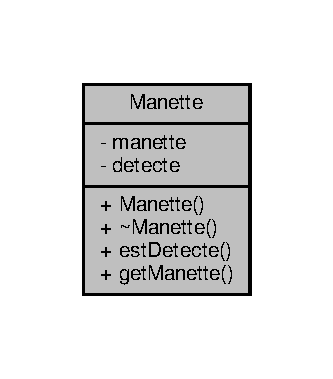
\includegraphics[width=160pt]{class_manette__coll__graph}
\end{center}
\end{figure}
\subsubsection*{Fonctions membres publiques}
\begin{DoxyCompactItemize}
\item 
\hyperlink{class_manette_a9a7b00a30cd6a7eea503c8bcfe5bbcbb}{Manette} (Q\+Object $\ast$parent=nullptr)
\begin{DoxyCompactList}\small\item\em Constructeur de la classe Gestionnaire\+Manette. La connexion entre les évènements de la manette et les méthodes cibles sont réalisées ici. \end{DoxyCompactList}\item 
\hyperlink{class_manette_a86a0cab49599b27d86c2e77f13fa54a2}{$\sim$\+Manette} ()
\item 
bool \hyperlink{class_manette_a035c0a43a11e91889891b3c874f0a58d}{est\+Detecte} () const
\begin{DoxyCompactList}\small\item\em est\+Detecte \end{DoxyCompactList}\item 
Q\+Gamepad $\ast$ \hyperlink{class_manette_a708eccb66e967e0fe575b19e9899ff5a}{get\+Manette} ()
\begin{DoxyCompactList}\small\item\em get\+Manette \end{DoxyCompactList}\end{DoxyCompactItemize}
\subsubsection*{Attributs privés}
\begin{DoxyCompactItemize}
\item 
Q\+Gamepad $\ast$ \hyperlink{class_manette_adc9690756093748bb851d4c1d3ba82ea}{manette}
\begin{DoxyCompactList}\small\item\em Contient la manette actuellement connectée. \end{DoxyCompactList}\item 
bool \hyperlink{class_manette_a2b9c2c380a7bce40d2c6353d534ba6a9}{detecte}
\begin{DoxyCompactList}\small\item\em \hyperlink{class_manette}{Manette} connectée, ou non. \end{DoxyCompactList}\end{DoxyCompactItemize}


\subsubsection{Description détaillée}
\begin{DoxyAuthor}{Auteur}
R\+E\+Y\+N\+I\+ER Jacques \& Nicolas B\+O\+F\+F\+R\+E\+DO
\end{DoxyAuthor}
\begin{DoxyVersion}{Version}
1.\+1
\end{DoxyVersion}
\begin{DoxyDate}{Date}
Jeudi 13 Juin 2019 
\end{DoxyDate}


\subsubsection{Documentation des constructeurs et destructeur}
\mbox{\Hypertarget{class_manette_a9a7b00a30cd6a7eea503c8bcfe5bbcbb}\label{class_manette_a9a7b00a30cd6a7eea503c8bcfe5bbcbb}} 
\index{Manette@{Manette}!Manette@{Manette}}
\index{Manette@{Manette}!Manette@{Manette}}
\paragraph{\texorpdfstring{Manette()}{Manette()}}
{\footnotesize\ttfamily Manette\+::\+Manette (\begin{DoxyParamCaption}\item[{Q\+Object $\ast$}]{parent = {\ttfamily nullptr} }\end{DoxyParamCaption})\hspace{0.3cm}{\ttfamily [explicit]}}


\begin{DoxyParams}{Paramètres}
{\em parent} & \\
\hline
\end{DoxyParams}


Références \hyperlink{class_manette_a2b9c2c380a7bce40d2c6353d534ba6a9}{detecte}, et \hyperlink{class_manette_adc9690756093748bb851d4c1d3ba82ea}{manette}.


\begin{DoxyCode}
00025                                 : QObject(parent), \hyperlink{class_manette_adc9690756093748bb851d4c1d3ba82ea}{manette}(\textcolor{keyword}{nullptr}), 
      \hyperlink{class_manette_a2b9c2c380a7bce40d2c6353d534ba6a9}{detecte}(\textcolor{keyword}{false})
00026 \{
00027 \textcolor{preprocessor}{    #ifndef QT\_NO\_DEBUG\_OUTPUT}
00028     QLoggingCategory::setFilterRules(QStringLiteral(\textcolor{stringliteral}{"qt.gamepad.debug=true"}));
00029 \textcolor{preprocessor}{    #endif}
00030 
00031     \textcolor{keyword}{auto} manettes = QGamepadManager::instance()->connectedGamepads();
00032 
00033     \textcolor{keywordflow}{if} (manettes.isEmpty())
00034     \{
00035         qDebug() << Q\_FUNC\_INFO << \textcolor{stringliteral}{"Aucune manette détectée !"};
00036         \hyperlink{class_manette_a2b9c2c380a7bce40d2c6353d534ba6a9}{detecte} = \textcolor{keyword}{false};
00037     \}
00038     \textcolor{keywordflow}{else}
00039     \{
00040         \hyperlink{class_manette_adc9690756093748bb851d4c1d3ba82ea}{manette} = \textcolor{keyword}{new} QGamepad(*manettes.begin(), \textcolor{keyword}{this});
00041         \hyperlink{class_manette_a2b9c2c380a7bce40d2c6353d534ba6a9}{detecte} = \textcolor{keyword}{true};
00042     \}
00043 \}
\end{DoxyCode}
\mbox{\Hypertarget{class_manette_a86a0cab49599b27d86c2e77f13fa54a2}\label{class_manette_a86a0cab49599b27d86c2e77f13fa54a2}} 
\index{Manette@{Manette}!````~Manette@{$\sim$\+Manette}}
\index{````~Manette@{$\sim$\+Manette}!Manette@{Manette}}
\paragraph{\texorpdfstring{$\sim$\+Manette()}{~Manette()}}
{\footnotesize\ttfamily Manette\+::$\sim$\+Manette (\begin{DoxyParamCaption}{ }\end{DoxyParamCaption})}


\begin{DoxyCode}
00046 \{
00047 
00048 \}
\end{DoxyCode}


\subsubsection{Documentation des fonctions membres}
\mbox{\Hypertarget{class_manette_a035c0a43a11e91889891b3c874f0a58d}\label{class_manette_a035c0a43a11e91889891b3c874f0a58d}} 
\index{Manette@{Manette}!est\+Detecte@{est\+Detecte}}
\index{est\+Detecte@{est\+Detecte}!Manette@{Manette}}
\paragraph{\texorpdfstring{est\+Detecte()}{estDetecte()}}
{\footnotesize\ttfamily bool Manette\+::est\+Detecte (\begin{DoxyParamCaption}{ }\end{DoxyParamCaption}) const}

Renvoie l\textquotesingle{}état de la manette (connectée, ou non).

\begin{DoxyReturn}{Renvoie}
detecte bool Etat de l\textquotesingle{}attribut detecte de l\textquotesingle{}objet.

detecte bool Indique si une manette est connectée ou non. 
\end{DoxyReturn}


Références \hyperlink{class_manette_a2b9c2c380a7bce40d2c6353d534ba6a9}{detecte}.



Référencé par \hyperlink{class_controle_rov_acc4d5fea26770217df978d43df2ad51e}{Controle\+Rov\+::\+Controle\+Rov()}, et \hyperlink{class_controle_rov_a9531520e50479fc2e339cd43f4c87066}{Controle\+Rov\+::est\+Controle\+Rov\+Disponible()}.


\begin{DoxyCode}
00056 \{
00057     \textcolor{keywordflow}{return} \hyperlink{class_manette_a2b9c2c380a7bce40d2c6353d534ba6a9}{detecte};
00058 \}
\end{DoxyCode}
\mbox{\Hypertarget{class_manette_a708eccb66e967e0fe575b19e9899ff5a}\label{class_manette_a708eccb66e967e0fe575b19e9899ff5a}} 
\index{Manette@{Manette}!get\+Manette@{get\+Manette}}
\index{get\+Manette@{get\+Manette}!Manette@{Manette}}
\paragraph{\texorpdfstring{get\+Manette()}{getManette()}}
{\footnotesize\ttfamily Q\+Gamepad $\ast$ Manette\+::get\+Manette (\begin{DoxyParamCaption}{ }\end{DoxyParamCaption})}

Renvoie la manette actuellement connectée.

\begin{DoxyReturn}{Renvoie}
manette Q\+Gamepad \hyperlink{class_manette}{Manette} actuellement connectée.

manette Q\+Gamepad$\ast$ \hyperlink{class_manette}{Manette} connectée. 
\end{DoxyReturn}


Références \hyperlink{class_manette_adc9690756093748bb851d4c1d3ba82ea}{manette}.



Référencé par \hyperlink{class_controle_rov_a400d5766b9acabb45c1af5f8b22bbe47}{Controle\+Rov\+::change\+Connexions()}, et \hyperlink{class_controle_rov_acc4d5fea26770217df978d43df2ad51e}{Controle\+Rov\+::\+Controle\+Rov()}.


\begin{DoxyCode}
00066 \{
00067     \textcolor{keywordflow}{return} \hyperlink{class_manette_adc9690756093748bb851d4c1d3ba82ea}{manette};
00068 \}
\end{DoxyCode}


\subsubsection{Documentation des données membres}
\mbox{\Hypertarget{class_manette_a2b9c2c380a7bce40d2c6353d534ba6a9}\label{class_manette_a2b9c2c380a7bce40d2c6353d534ba6a9}} 
\index{Manette@{Manette}!detecte@{detecte}}
\index{detecte@{detecte}!Manette@{Manette}}
\paragraph{\texorpdfstring{detecte}{detecte}}
{\footnotesize\ttfamily bool Manette\+::detecte\hspace{0.3cm}{\ttfamily [private]}}



Référencé par \hyperlink{class_manette_a035c0a43a11e91889891b3c874f0a58d}{est\+Detecte()}, et \hyperlink{class_manette_a9a7b00a30cd6a7eea503c8bcfe5bbcbb}{Manette()}.

\mbox{\Hypertarget{class_manette_adc9690756093748bb851d4c1d3ba82ea}\label{class_manette_adc9690756093748bb851d4c1d3ba82ea}} 
\index{Manette@{Manette}!manette@{manette}}
\index{manette@{manette}!Manette@{Manette}}
\paragraph{\texorpdfstring{manette}{manette}}
{\footnotesize\ttfamily Q\+Gamepad$\ast$ Manette\+::manette\hspace{0.3cm}{\ttfamily [private]}}



Référencé par \hyperlink{class_manette_a708eccb66e967e0fe575b19e9899ff5a}{get\+Manette()}, et \hyperlink{class_manette_a9a7b00a30cd6a7eea503c8bcfe5bbcbb}{Manette()}.



La documentation de cette classe a été générée à partir des fichiers suivants \+:\begin{DoxyCompactItemize}
\item 
\hyperlink{manette_8h}{manette.\+h}\item 
\hyperlink{manette_8cpp}{manette.\+cpp}\end{DoxyCompactItemize}

\hypertarget{class_mesures}{}\subsection{Référence de la classe Mesures}
\label{class_mesures}\index{Mesures@{Mesures}}


Déclaration de la classe \hyperlink{class_mesures}{Mesures}. Gestion des mesures des capteurs (température, irradiation, et distance).  




{\ttfamily \#include $<$mesures.\+h$>$}



Graphe de collaboration de Mesures\+:
\nopagebreak
\begin{figure}[H]
\begin{center}
\leavevmode
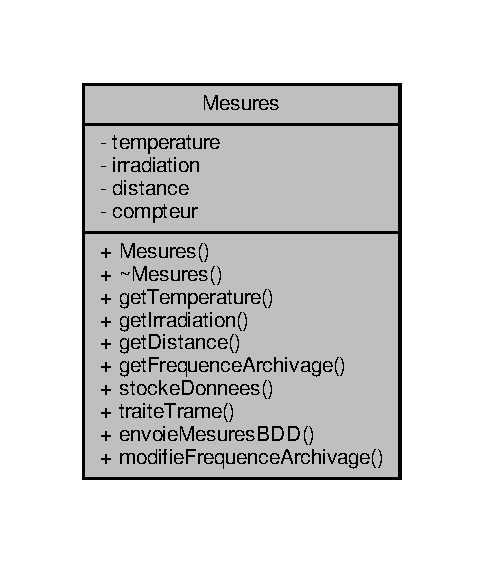
\includegraphics[width=232pt]{class_mesures__coll__graph}
\end{center}
\end{figure}
\subsubsection*{Connecteurs publics}
\begin{DoxyCompactItemize}
\item 
void \hyperlink{class_mesures_a43b121b67418802b3332b195d8541481}{traite\+Trame} (Q\+String trame)
\begin{DoxyCompactList}\small\item\em Vérifie la validité, et découpe la trame reçue. \end{DoxyCompactList}\item 
void \hyperlink{class_mesures_a9eb8d49c9f60b3801110a5c3d0c50149}{envoie\+Mesures\+B\+DD} ()
\begin{DoxyCompactList}\small\item\em Envoie un signal toutes les 30 secondes contenant la température et l\textquotesingle{}irradiation. \end{DoxyCompactList}\item 
void \hyperlink{class_mesures_ac1d2ea97f648264ebd690fba8f7020cc}{modifie\+Frequence\+Archivage} (int)
\begin{DoxyCompactList}\small\item\em Modifie l\textquotesingle{}interval du timer correspondant à l\textquotesingle{}archivage des mesures dans la B\+DD. \end{DoxyCompactList}\end{DoxyCompactItemize}
\subsubsection*{Signaux}
\begin{DoxyCompactItemize}
\item 
void \hyperlink{class_mesures_a8a6e4db8850930d8e4e96c98d5aa95b8}{irradiation\+Actualisee} (double)
\begin{DoxyCompactList}\small\item\em Signal émis lorsqu\textquotesingle{}une nouvelle valeur d\textquotesingle{}irradiation est reçue. \end{DoxyCompactList}\item 
void \hyperlink{class_mesures_ab13d5e64ff21fd869fe347ec1c5a246f}{temperature\+Actualisee} (double)
\begin{DoxyCompactList}\small\item\em Signal émis lorsqu\textquotesingle{}une nouvelle valeur de température est reçue. \end{DoxyCompactList}\item 
void \hyperlink{class_mesures_a6073f147fb08d7c5cc2ce1c9880becbe}{distance\+Actualisee} (double)
\begin{DoxyCompactList}\small\item\em Signal émis lorsqu\textquotesingle{}une nouvelle valeur de distance est reçue. \end{DoxyCompactList}\item 
void \hyperlink{class_mesures_a97d8dbd7742519d1f3ce959661d8aede}{mesures\+B\+D\+D\+Prete} (double \hyperlink{class_mesures_a2688d0da4acf9d91ea0befd6ed0bd140}{temperature}, double \hyperlink{class_mesures_a77cde7672dac5e544b7288364ec7c7b5}{irradiation})
\begin{DoxyCompactList}\small\item\em Signal émis toutes les x secondes visant à stocker les valeurs de température et d\textquotesingle{}irradiation (en argument) dans la B\+DD. \end{DoxyCompactList}\end{DoxyCompactItemize}
\subsubsection*{Fonctions membres publiques}
\begin{DoxyCompactItemize}
\item 
\hyperlink{class_mesures_aa24ed1e055242fab5adab3f8f057c9b1}{Mesures} (Q\+Object $\ast$parent=nullptr)
\begin{DoxyCompactList}\small\item\em Constructeur de la classe \hyperlink{class_mesures}{Mesures}. \end{DoxyCompactList}\item 
\hyperlink{class_mesures_a4bb192b80fbf2c0f9aea5911ce29c652}{$\sim$\+Mesures} ()
\begin{DoxyCompactList}\small\item\em Destructeur de la classe \hyperlink{class_mesures}{Mesures}. \end{DoxyCompactList}\item 
double \hyperlink{class_mesures_a5e5e61c6bbdd2fd891b66ee494183dcd}{get\+Temperature} () const
\begin{DoxyCompactList}\small\item\em Retourne la température stockée dans l\textquotesingle{}objet. \end{DoxyCompactList}\item 
double \hyperlink{class_mesures_af260c8f685e3519681b3ca0086d70b31}{get\+Irradiation} () const
\begin{DoxyCompactList}\small\item\em Retourne le taux d\textquotesingle{}irradiation stocké dans l\textquotesingle{}objet. \end{DoxyCompactList}\item 
double \hyperlink{class_mesures_aa40d78428855bab861cc9a57582c8d42}{get\+Distance} () const
\begin{DoxyCompactList}\small\item\em Renvoie le dernier relevé du capteur de proximité. \end{DoxyCompactList}\item 
int \hyperlink{class_mesures_ae969e38402b8d19fe9b484f368200578}{get\+Frequence\+Archivage} () const
\begin{DoxyCompactList}\small\item\em Renvoie la fréquence d\textquotesingle{}archivage des données. \end{DoxyCompactList}\item 
void \hyperlink{class_mesures_a77652c2332a9234bf08b463d1d389aa5}{stocke\+Donnees} (Q\+String type, Q\+String donnee)
\begin{DoxyCompactList}\small\item\em Stocke la donnee passée en argument. \end{DoxyCompactList}\end{DoxyCompactItemize}
\subsubsection*{Attributs privés}
\begin{DoxyCompactItemize}
\item 
double \hyperlink{class_mesures_a2688d0da4acf9d91ea0befd6ed0bd140}{temperature}
\begin{DoxyCompactList}\small\item\em Dernière température relevée. \end{DoxyCompactList}\item 
double \hyperlink{class_mesures_a77cde7672dac5e544b7288364ec7c7b5}{irradiation}
\begin{DoxyCompactList}\small\item\em Dernier taux d\textquotesingle{}irradiation relevé. \end{DoxyCompactList}\item 
double \hyperlink{class_mesures_a276f71168b1dcecf2051631d19aa8eeb}{distance}
\begin{DoxyCompactList}\small\item\em Dernière mesure du capteur de proximité relevé. \end{DoxyCompactList}\item 
Q\+Timer $\ast$ \hyperlink{class_mesures_a89af5f279d21cf10f5d6bd58bbc33173}{compteur}
\begin{DoxyCompactList}\small\item\em Compteur envoyant toutes les x secondes un signal timeout. \end{DoxyCompactList}\end{DoxyCompactItemize}


\subsubsection{Description détaillée}
\begin{DoxyAuthor}{Auteur}
R\+E\+Y\+N\+I\+ER Jacques \& Nicolas B\+O\+F\+F\+R\+E\+DO
\end{DoxyAuthor}
\begin{DoxyVersion}{Version}
1.\+1
\end{DoxyVersion}
\begin{DoxyDate}{Date}
Jeudi 13 Juin 2019 
\end{DoxyDate}


\subsubsection{Documentation des constructeurs et destructeur}
\mbox{\Hypertarget{class_mesures_aa24ed1e055242fab5adab3f8f057c9b1}\label{class_mesures_aa24ed1e055242fab5adab3f8f057c9b1}} 
\index{Mesures@{Mesures}!Mesures@{Mesures}}
\index{Mesures@{Mesures}!Mesures@{Mesures}}
\paragraph{\texorpdfstring{Mesures()}{Mesures()}}
{\footnotesize\ttfamily Mesures\+::\+Mesures (\begin{DoxyParamCaption}\item[{Q\+Object $\ast$}]{parent = {\ttfamily nullptr} }\end{DoxyParamCaption})\hspace{0.3cm}{\ttfamily [explicit]}}

Crée un compteur émettant un signal toutes les 30 secondes (modifiable par l\textquotesingle{}utilisateur), permettant l\textquotesingle{}envoi des mesures dans la B\+DD.


\begin{DoxyParams}{Paramètres}
{\em parent} & Q\+Object$\ast$ \\
\hline
\end{DoxyParams}


Références \hyperlink{class_mesures_a89af5f279d21cf10f5d6bd58bbc33173}{compteur}, et \hyperlink{class_mesures_a9eb8d49c9f60b3801110a5c3d0c50149}{envoie\+Mesures\+B\+D\+D()}.


\begin{DoxyCode}
00023                                 : QObject(parent), \hyperlink{class_mesures_a2688d0da4acf9d91ea0befd6ed0bd140}{temperature}(-999.0), 
      \hyperlink{class_mesures_a77cde7672dac5e544b7288364ec7c7b5}{irradiation}(-999.0), \hyperlink{class_mesures_a276f71168b1dcecf2051631d19aa8eeb}{distance}(-999.0)
00024 \{
00025     \hyperlink{class_mesures_a89af5f279d21cf10f5d6bd58bbc33173}{compteur} = \textcolor{keyword}{new} QTimer(\textcolor{keyword}{this});
00026     connect(\hyperlink{class_mesures_a89af5f279d21cf10f5d6bd58bbc33173}{compteur}, SIGNAL(timeout()), \textcolor{keyword}{this}, SLOT(\hyperlink{class_mesures_a9eb8d49c9f60b3801110a5c3d0c50149}{envoieMesuresBDD}()));
00027     \hyperlink{class_mesures_a89af5f279d21cf10f5d6bd58bbc33173}{compteur}->start(30000);
00028 \}
\end{DoxyCode}
\mbox{\Hypertarget{class_mesures_a4bb192b80fbf2c0f9aea5911ce29c652}\label{class_mesures_a4bb192b80fbf2c0f9aea5911ce29c652}} 
\index{Mesures@{Mesures}!````~Mesures@{$\sim$\+Mesures}}
\index{````~Mesures@{$\sim$\+Mesures}!Mesures@{Mesures}}
\paragraph{\texorpdfstring{$\sim$\+Mesures()}{~Mesures()}}
{\footnotesize\ttfamily Mesures\+::$\sim$\+Mesures (\begin{DoxyParamCaption}{ }\end{DoxyParamCaption})}


\begin{DoxyCode}
00035 \{
00036 
00037 \}
\end{DoxyCode}


\subsubsection{Documentation des fonctions membres}
\mbox{\Hypertarget{class_mesures_a6073f147fb08d7c5cc2ce1c9880becbe}\label{class_mesures_a6073f147fb08d7c5cc2ce1c9880becbe}} 
\index{Mesures@{Mesures}!distance\+Actualisee@{distance\+Actualisee}}
\index{distance\+Actualisee@{distance\+Actualisee}!Mesures@{Mesures}}
\paragraph{\texorpdfstring{distance\+Actualisee}{distanceActualisee}}
{\footnotesize\ttfamily void Mesures\+::distance\+Actualisee (\begin{DoxyParamCaption}\item[{double}]{ }\end{DoxyParamCaption})\hspace{0.3cm}{\ttfamily [signal]}}



Référencé par \hyperlink{class_mesures_a77652c2332a9234bf08b463d1d389aa5}{stocke\+Donnees()}.

\mbox{\Hypertarget{class_mesures_a9eb8d49c9f60b3801110a5c3d0c50149}\label{class_mesures_a9eb8d49c9f60b3801110a5c3d0c50149}} 
\index{Mesures@{Mesures}!envoie\+Mesures\+B\+DD@{envoie\+Mesures\+B\+DD}}
\index{envoie\+Mesures\+B\+DD@{envoie\+Mesures\+B\+DD}!Mesures@{Mesures}}
\paragraph{\texorpdfstring{envoie\+Mesures\+B\+DD}{envoieMesuresBDD}}
{\footnotesize\ttfamily void Mesures\+::envoie\+Mesures\+B\+DD (\begin{DoxyParamCaption}{ }\end{DoxyParamCaption})\hspace{0.3cm}{\ttfamily [slot]}}

Envoie un signal comprenant les mesures de température et d\textquotesingle{}irradiation à destination de la B\+DD, émis toutes les x secondes (fréquence d\textquotesingle{}archivage). 

Références \hyperlink{class_mesures_a77cde7672dac5e544b7288364ec7c7b5}{irradiation}, \hyperlink{class_mesures_a97d8dbd7742519d1f3ce959661d8aede}{mesures\+B\+D\+D\+Prete()}, et \hyperlink{class_mesures_a2688d0da4acf9d91ea0befd6ed0bd140}{temperature}.



Référencé par \hyperlink{class_mesures_aa24ed1e055242fab5adab3f8f057c9b1}{Mesures()}.


\begin{DoxyCode}
00150 \{
00151     emit \hyperlink{class_mesures_a97d8dbd7742519d1f3ce959661d8aede}{mesuresBDDPrete}(this->\hyperlink{class_mesures_a2688d0da4acf9d91ea0befd6ed0bd140}{temperature}, this->
      \hyperlink{class_mesures_a77cde7672dac5e544b7288364ec7c7b5}{irradiation});
00152 \}
\end{DoxyCode}
\mbox{\Hypertarget{class_mesures_aa40d78428855bab861cc9a57582c8d42}\label{class_mesures_aa40d78428855bab861cc9a57582c8d42}} 
\index{Mesures@{Mesures}!get\+Distance@{get\+Distance}}
\index{get\+Distance@{get\+Distance}!Mesures@{Mesures}}
\paragraph{\texorpdfstring{get\+Distance()}{getDistance()}}
{\footnotesize\ttfamily Mesures\+::get\+Distance (\begin{DoxyParamCaption}{ }\end{DoxyParamCaption}) const}

\begin{DoxyReturn}{Renvoie}
distance double Dernier relevé du capteur de proximité. 
\end{DoxyReturn}


Références \hyperlink{class_mesures_a276f71168b1dcecf2051631d19aa8eeb}{distance}.


\begin{DoxyCode}
00065 \{
00066     \textcolor{keywordflow}{return} this->\hyperlink{class_mesures_a276f71168b1dcecf2051631d19aa8eeb}{distance};
00067 \}
\end{DoxyCode}
\mbox{\Hypertarget{class_mesures_ae969e38402b8d19fe9b484f368200578}\label{class_mesures_ae969e38402b8d19fe9b484f368200578}} 
\index{Mesures@{Mesures}!get\+Frequence\+Archivage@{get\+Frequence\+Archivage}}
\index{get\+Frequence\+Archivage@{get\+Frequence\+Archivage}!Mesures@{Mesures}}
\paragraph{\texorpdfstring{get\+Frequence\+Archivage()}{getFrequenceArchivage()}}
{\footnotesize\ttfamily int Mesures\+::get\+Frequence\+Archivage (\begin{DoxyParamCaption}{ }\end{DoxyParamCaption}) const}

Renvoie la fréquence d\textquotesingle{}archivage des mesures dans la B\+DD en secondes.

\begin{DoxyReturn}{Renvoie}
frequence int Fréquence d\textquotesingle{}archivage en secondes. 
\end{DoxyReturn}


Références \hyperlink{class_mesures_a89af5f279d21cf10f5d6bd58bbc33173}{compteur}.



Référencé par \hyperlink{class_i_h_m_rov_aed451139ac09ef18b7c92637761d80ce}{I\+H\+M\+Rov\+::creer\+Fenetre\+Parametres()}.


\begin{DoxyCode}
00075 \{
00076     \textcolor{keywordflow}{return} (\hyperlink{class_mesures_a89af5f279d21cf10f5d6bd58bbc33173}{compteur}->interval() / 1000);
00077 \}
\end{DoxyCode}
\mbox{\Hypertarget{class_mesures_af260c8f685e3519681b3ca0086d70b31}\label{class_mesures_af260c8f685e3519681b3ca0086d70b31}} 
\index{Mesures@{Mesures}!get\+Irradiation@{get\+Irradiation}}
\index{get\+Irradiation@{get\+Irradiation}!Mesures@{Mesures}}
\paragraph{\texorpdfstring{get\+Irradiation()}{getIrradiation()}}
{\footnotesize\ttfamily Mesures\+::get\+Irradiation (\begin{DoxyParamCaption}{ }\end{DoxyParamCaption}) const}

Renvoie le dernier taux d\textquotesingle{}irradiation reçu.

\begin{DoxyReturn}{Renvoie}
irradiation int Dernier taux d\textquotesingle{}irradiation relevé. 
\end{DoxyReturn}


Références \hyperlink{class_mesures_a77cde7672dac5e544b7288364ec7c7b5}{irradiation}.


\begin{DoxyCode}
00055 \{
00056     \textcolor{keywordflow}{return} this->\hyperlink{class_mesures_a77cde7672dac5e544b7288364ec7c7b5}{irradiation};
00057 \}
\end{DoxyCode}
\mbox{\Hypertarget{class_mesures_a5e5e61c6bbdd2fd891b66ee494183dcd}\label{class_mesures_a5e5e61c6bbdd2fd891b66ee494183dcd}} 
\index{Mesures@{Mesures}!get\+Temperature@{get\+Temperature}}
\index{get\+Temperature@{get\+Temperature}!Mesures@{Mesures}}
\paragraph{\texorpdfstring{get\+Temperature()}{getTemperature()}}
{\footnotesize\ttfamily Mesures\+::get\+Temperature (\begin{DoxyParamCaption}{ }\end{DoxyParamCaption}) const}

Renvoie la dernière température reçue.

\begin{DoxyReturn}{Renvoie}
temperature int Dernière température relevée. 
\end{DoxyReturn}


Références \hyperlink{class_mesures_a2688d0da4acf9d91ea0befd6ed0bd140}{temperature}.


\begin{DoxyCode}
00045 \{
00046     \textcolor{keywordflow}{return} this->\hyperlink{class_mesures_a2688d0da4acf9d91ea0befd6ed0bd140}{temperature};
00047 \}
\end{DoxyCode}
\mbox{\Hypertarget{class_mesures_a8a6e4db8850930d8e4e96c98d5aa95b8}\label{class_mesures_a8a6e4db8850930d8e4e96c98d5aa95b8}} 
\index{Mesures@{Mesures}!irradiation\+Actualisee@{irradiation\+Actualisee}}
\index{irradiation\+Actualisee@{irradiation\+Actualisee}!Mesures@{Mesures}}
\paragraph{\texorpdfstring{irradiation\+Actualisee}{irradiationActualisee}}
{\footnotesize\ttfamily void Mesures\+::irradiation\+Actualisee (\begin{DoxyParamCaption}\item[{double}]{ }\end{DoxyParamCaption})\hspace{0.3cm}{\ttfamily [signal]}}



Référencé par \hyperlink{class_mesures_a77652c2332a9234bf08b463d1d389aa5}{stocke\+Donnees()}.

\mbox{\Hypertarget{class_mesures_a97d8dbd7742519d1f3ce959661d8aede}\label{class_mesures_a97d8dbd7742519d1f3ce959661d8aede}} 
\index{Mesures@{Mesures}!mesures\+B\+D\+D\+Prete@{mesures\+B\+D\+D\+Prete}}
\index{mesures\+B\+D\+D\+Prete@{mesures\+B\+D\+D\+Prete}!Mesures@{Mesures}}
\paragraph{\texorpdfstring{mesures\+B\+D\+D\+Prete}{mesuresBDDPrete}}
{\footnotesize\ttfamily void Mesures\+::mesures\+B\+D\+D\+Prete (\begin{DoxyParamCaption}\item[{double}]{temperature,  }\item[{double}]{irradiation }\end{DoxyParamCaption})\hspace{0.3cm}{\ttfamily [signal]}}



Référencé par \hyperlink{class_mesures_a9eb8d49c9f60b3801110a5c3d0c50149}{envoie\+Mesures\+B\+D\+D()}.

\mbox{\Hypertarget{class_mesures_ac1d2ea97f648264ebd690fba8f7020cc}\label{class_mesures_ac1d2ea97f648264ebd690fba8f7020cc}} 
\index{Mesures@{Mesures}!modifie\+Frequence\+Archivage@{modifie\+Frequence\+Archivage}}
\index{modifie\+Frequence\+Archivage@{modifie\+Frequence\+Archivage}!Mesures@{Mesures}}
\paragraph{\texorpdfstring{modifie\+Frequence\+Archivage}{modifieFrequenceArchivage}}
{\footnotesize\ttfamily void Mesures\+::modifie\+Frequence\+Archivage (\begin{DoxyParamCaption}\item[{int}]{frequence }\end{DoxyParamCaption})\hspace{0.3cm}{\ttfamily [slot]}}

Modifie la fréquence.


\begin{DoxyParams}{Paramètres}
{\em frequence} & \\
\hline
\end{DoxyParams}


Références \hyperlink{class_mesures_a89af5f279d21cf10f5d6bd58bbc33173}{compteur}.



Référencé par \hyperlink{class_i_h_m_rov_aed451139ac09ef18b7c92637761d80ce}{I\+H\+M\+Rov\+::creer\+Fenetre\+Parametres()}.


\begin{DoxyCode}
00160 \{
00161     \hyperlink{class_mesures_a89af5f279d21cf10f5d6bd58bbc33173}{compteur}->setInterval(frequence * 1000);
00162 \}
\end{DoxyCode}
\mbox{\Hypertarget{class_mesures_a77652c2332a9234bf08b463d1d389aa5}\label{class_mesures_a77652c2332a9234bf08b463d1d389aa5}} 
\index{Mesures@{Mesures}!stocke\+Donnees@{stocke\+Donnees}}
\index{stocke\+Donnees@{stocke\+Donnees}!Mesures@{Mesures}}
\paragraph{\texorpdfstring{stocke\+Donnees()}{stockeDonnees()}}
{\footnotesize\ttfamily void Mesures\+::stocke\+Donnees (\begin{DoxyParamCaption}\item[{Q\+String}]{type,  }\item[{Q\+String}]{donnee }\end{DoxyParamCaption})}

Stocke les donnees passés en argument dans l\textquotesingle{}objet mesures.


\begin{DoxyParams}{Paramètres}
{\em type} & Q\+String Type de donnée à stocker. \\
\hline
{\em donnee} & Q\+String Valeur de la donnée à stocker. \\
\hline
\end{DoxyParams}


Références \hyperlink{class_mesures_a276f71168b1dcecf2051631d19aa8eeb}{distance}, \hyperlink{class_mesures_a6073f147fb08d7c5cc2ce1c9880becbe}{distance\+Actualisee()}, \hyperlink{class_mesures_a77cde7672dac5e544b7288364ec7c7b5}{irradiation}, \hyperlink{class_mesures_a8a6e4db8850930d8e4e96c98d5aa95b8}{irradiation\+Actualisee()}, \hyperlink{class_mesures_a2688d0da4acf9d91ea0befd6ed0bd140}{temperature}, et \hyperlink{class_mesures_ab13d5e64ff21fd869fe347ec1c5a246f}{temperature\+Actualisee()}.



Référencé par \hyperlink{class_mesures_a43b121b67418802b3332b195d8541481}{traite\+Trame()}.


\begin{DoxyCode}
00125 \{
00126     \textcolor{keywordflow}{if} (type == \textcolor{stringliteral}{"irradiation"})
00127     \{
00128         this->\hyperlink{class_mesures_a77cde7672dac5e544b7288364ec7c7b5}{irradiation} = donnee.toDouble();
00129         emit \hyperlink{class_mesures_a8a6e4db8850930d8e4e96c98d5aa95b8}{irradiationActualisee}(this->\hyperlink{class_mesures_a77cde7672dac5e544b7288364ec7c7b5}{irradiation});
00130     \}
00131 
00132     \textcolor{keywordflow}{if} (type == \textcolor{stringliteral}{"temperature"})
00133     \{
00134         this->\hyperlink{class_mesures_a2688d0da4acf9d91ea0befd6ed0bd140}{temperature} = donnee.toDouble();
00135         emit \hyperlink{class_mesures_ab13d5e64ff21fd869fe347ec1c5a246f}{temperatureActualisee}(this->\hyperlink{class_mesures_a2688d0da4acf9d91ea0befd6ed0bd140}{temperature});
00136     \}
00137 
00138     \textcolor{keywordflow}{if} (type == \textcolor{stringliteral}{"distance"})
00139     \{
00140         this->\hyperlink{class_mesures_a276f71168b1dcecf2051631d19aa8eeb}{distance} = donnee.toDouble();
00141         emit \hyperlink{class_mesures_a6073f147fb08d7c5cc2ce1c9880becbe}{distanceActualisee}(this->\hyperlink{class_mesures_a276f71168b1dcecf2051631d19aa8eeb}{distance});
00142     \}
00143 \}
\end{DoxyCode}
\mbox{\Hypertarget{class_mesures_ab13d5e64ff21fd869fe347ec1c5a246f}\label{class_mesures_ab13d5e64ff21fd869fe347ec1c5a246f}} 
\index{Mesures@{Mesures}!temperature\+Actualisee@{temperature\+Actualisee}}
\index{temperature\+Actualisee@{temperature\+Actualisee}!Mesures@{Mesures}}
\paragraph{\texorpdfstring{temperature\+Actualisee}{temperatureActualisee}}
{\footnotesize\ttfamily void Mesures\+::temperature\+Actualisee (\begin{DoxyParamCaption}\item[{double}]{ }\end{DoxyParamCaption})\hspace{0.3cm}{\ttfamily [signal]}}



Référencé par \hyperlink{class_mesures_a77652c2332a9234bf08b463d1d389aa5}{stocke\+Donnees()}.

\mbox{\Hypertarget{class_mesures_a43b121b67418802b3332b195d8541481}\label{class_mesures_a43b121b67418802b3332b195d8541481}} 
\index{Mesures@{Mesures}!traite\+Trame@{traite\+Trame}}
\index{traite\+Trame@{traite\+Trame}!Mesures@{Mesures}}
\paragraph{\texorpdfstring{traite\+Trame}{traiteTrame}}
{\footnotesize\ttfamily void Mesures\+::traite\+Trame (\begin{DoxyParamCaption}\item[{Q\+String}]{trame }\end{DoxyParamCaption})\hspace{0.3cm}{\ttfamily [slot]}}


\begin{DoxyParams}{Paramètres}
{\em trame} & Q\+String Trame reçue. \\
\hline
\end{DoxyParams}


Références \hyperlink{class_mesures_a77652c2332a9234bf08b463d1d389aa5}{stocke\+Donnees()}.


\begin{DoxyCode}
00085 \{
00086     \textcolor{keywordtype}{bool} trameValide = \textcolor{keyword}{true};
00087 
00088     \textcolor{keywordflow}{if} (trame.startsWith(\textcolor{stringliteral}{"$"}) && trame.endsWith(\textcolor{stringliteral}{"\(\backslash\)n"}))
00089     \{
00090         trame.remove(QChar(\textcolor{charliteral}{'$'}));
00091         trame.remove(QChar(\textcolor{charliteral}{'\(\backslash\)n'}));
00092 
00093         \textcolor{keywordflow}{for}(\textcolor{keywordtype}{int} i = 1; i < trame.length(); i++)     \textcolor{comment}{// Parcours la trame et vérifie si le contenu après le
       caractère de type est bien un chiffre (filtre les erreurs exemple : "$TX4\(\backslash\)n").}
00094         \{
00095             \textcolor{keywordflow}{if}(!trame[i].isDigit() && trame[i] != \textcolor{stringliteral}{"."} && trame[i] != \textcolor{stringliteral}{"-"})
00096                 trameValide = \textcolor{keyword}{false};
00097         \}
00098     \}
00099     \textcolor{keywordflow}{else}
00100         trameValide = \textcolor{keyword}{false};
00101 
00102     \textcolor{keywordflow}{if}(trameValide)
00103     \{
00104         \textcolor{keywordflow}{if}(trame.startsWith(\textcolor{charliteral}{'T'}))
00105             \hyperlink{class_mesures_a77652c2332a9234bf08b463d1d389aa5}{stockeDonnees}(\textcolor{stringliteral}{"temperature"}, trame.remove(\textcolor{charliteral}{'T'}));
00106         \textcolor{keywordflow}{else} \textcolor{keywordflow}{if}(trame.startsWith(\textcolor{charliteral}{'R'}))
00107             \hyperlink{class_mesures_a77652c2332a9234bf08b463d1d389aa5}{stockeDonnees}(\textcolor{stringliteral}{"irradiation"}, trame.remove(\textcolor{charliteral}{'R'}));
00108         \textcolor{keywordflow}{else} \textcolor{keywordflow}{if}(trame.startsWith(\textcolor{charliteral}{'D'}))
00109             \hyperlink{class_mesures_a77652c2332a9234bf08b463d1d389aa5}{stockeDonnees}(\textcolor{stringliteral}{"distance"}, trame.remove(\textcolor{charliteral}{'D'}));
00110         \textcolor{keywordflow}{else}
00111             trameValide = \textcolor{keyword}{false};
00112     \}
00113 
00114     \textcolor{keywordflow}{if}(!trameValide)
00115         qDebug() << Q\_FUNC\_INFO << \textcolor{stringliteral}{"ERREUR ! Trame invalide"};
00116 \}
\end{DoxyCode}


\subsubsection{Documentation des données membres}
\mbox{\Hypertarget{class_mesures_a89af5f279d21cf10f5d6bd58bbc33173}\label{class_mesures_a89af5f279d21cf10f5d6bd58bbc33173}} 
\index{Mesures@{Mesures}!compteur@{compteur}}
\index{compteur@{compteur}!Mesures@{Mesures}}
\paragraph{\texorpdfstring{compteur}{compteur}}
{\footnotesize\ttfamily Q\+Timer$\ast$ Mesures\+::compteur\hspace{0.3cm}{\ttfamily [private]}}



Référencé par \hyperlink{class_mesures_ae969e38402b8d19fe9b484f368200578}{get\+Frequence\+Archivage()}, \hyperlink{class_mesures_aa24ed1e055242fab5adab3f8f057c9b1}{Mesures()}, et \hyperlink{class_mesures_ac1d2ea97f648264ebd690fba8f7020cc}{modifie\+Frequence\+Archivage()}.

\mbox{\Hypertarget{class_mesures_a276f71168b1dcecf2051631d19aa8eeb}\label{class_mesures_a276f71168b1dcecf2051631d19aa8eeb}} 
\index{Mesures@{Mesures}!distance@{distance}}
\index{distance@{distance}!Mesures@{Mesures}}
\paragraph{\texorpdfstring{distance}{distance}}
{\footnotesize\ttfamily double Mesures\+::distance\hspace{0.3cm}{\ttfamily [private]}}



Référencé par \hyperlink{class_mesures_aa40d78428855bab861cc9a57582c8d42}{get\+Distance()}, et \hyperlink{class_mesures_a77652c2332a9234bf08b463d1d389aa5}{stocke\+Donnees()}.

\mbox{\Hypertarget{class_mesures_a77cde7672dac5e544b7288364ec7c7b5}\label{class_mesures_a77cde7672dac5e544b7288364ec7c7b5}} 
\index{Mesures@{Mesures}!irradiation@{irradiation}}
\index{irradiation@{irradiation}!Mesures@{Mesures}}
\paragraph{\texorpdfstring{irradiation}{irradiation}}
{\footnotesize\ttfamily double Mesures\+::irradiation\hspace{0.3cm}{\ttfamily [private]}}



Référencé par \hyperlink{class_mesures_a9eb8d49c9f60b3801110a5c3d0c50149}{envoie\+Mesures\+B\+D\+D()}, \hyperlink{class_mesures_af260c8f685e3519681b3ca0086d70b31}{get\+Irradiation()}, et \hyperlink{class_mesures_a77652c2332a9234bf08b463d1d389aa5}{stocke\+Donnees()}.

\mbox{\Hypertarget{class_mesures_a2688d0da4acf9d91ea0befd6ed0bd140}\label{class_mesures_a2688d0da4acf9d91ea0befd6ed0bd140}} 
\index{Mesures@{Mesures}!temperature@{temperature}}
\index{temperature@{temperature}!Mesures@{Mesures}}
\paragraph{\texorpdfstring{temperature}{temperature}}
{\footnotesize\ttfamily double Mesures\+::temperature\hspace{0.3cm}{\ttfamily [private]}}



Référencé par \hyperlink{class_mesures_a9eb8d49c9f60b3801110a5c3d0c50149}{envoie\+Mesures\+B\+D\+D()}, \hyperlink{class_mesures_a5e5e61c6bbdd2fd891b66ee494183dcd}{get\+Temperature()}, et \hyperlink{class_mesures_a77652c2332a9234bf08b463d1d389aa5}{stocke\+Donnees()}.



La documentation de cette classe a été générée à partir des fichiers suivants \+:\begin{DoxyCompactItemize}
\item 
\hyperlink{mesures_8h}{mesures.\+h}\item 
\hyperlink{mesures_8cpp}{mesures.\+cpp}\end{DoxyCompactItemize}

\hypertarget{class_rov}{}\subsection{Référence de la classe Rov}
\label{class_rov}\index{Rov@{Rov}}


Déclaration de la classe \hyperlink{class_rov}{Rov}. Gestion des liaisons entre les différentes classes, et paramètres de la campagne et de la B\+DD.  




{\ttfamily \#include $<$rov.\+h$>$}



Graphe de collaboration de Rov\+:
\nopagebreak
\begin{figure}[H]
\begin{center}
\leavevmode
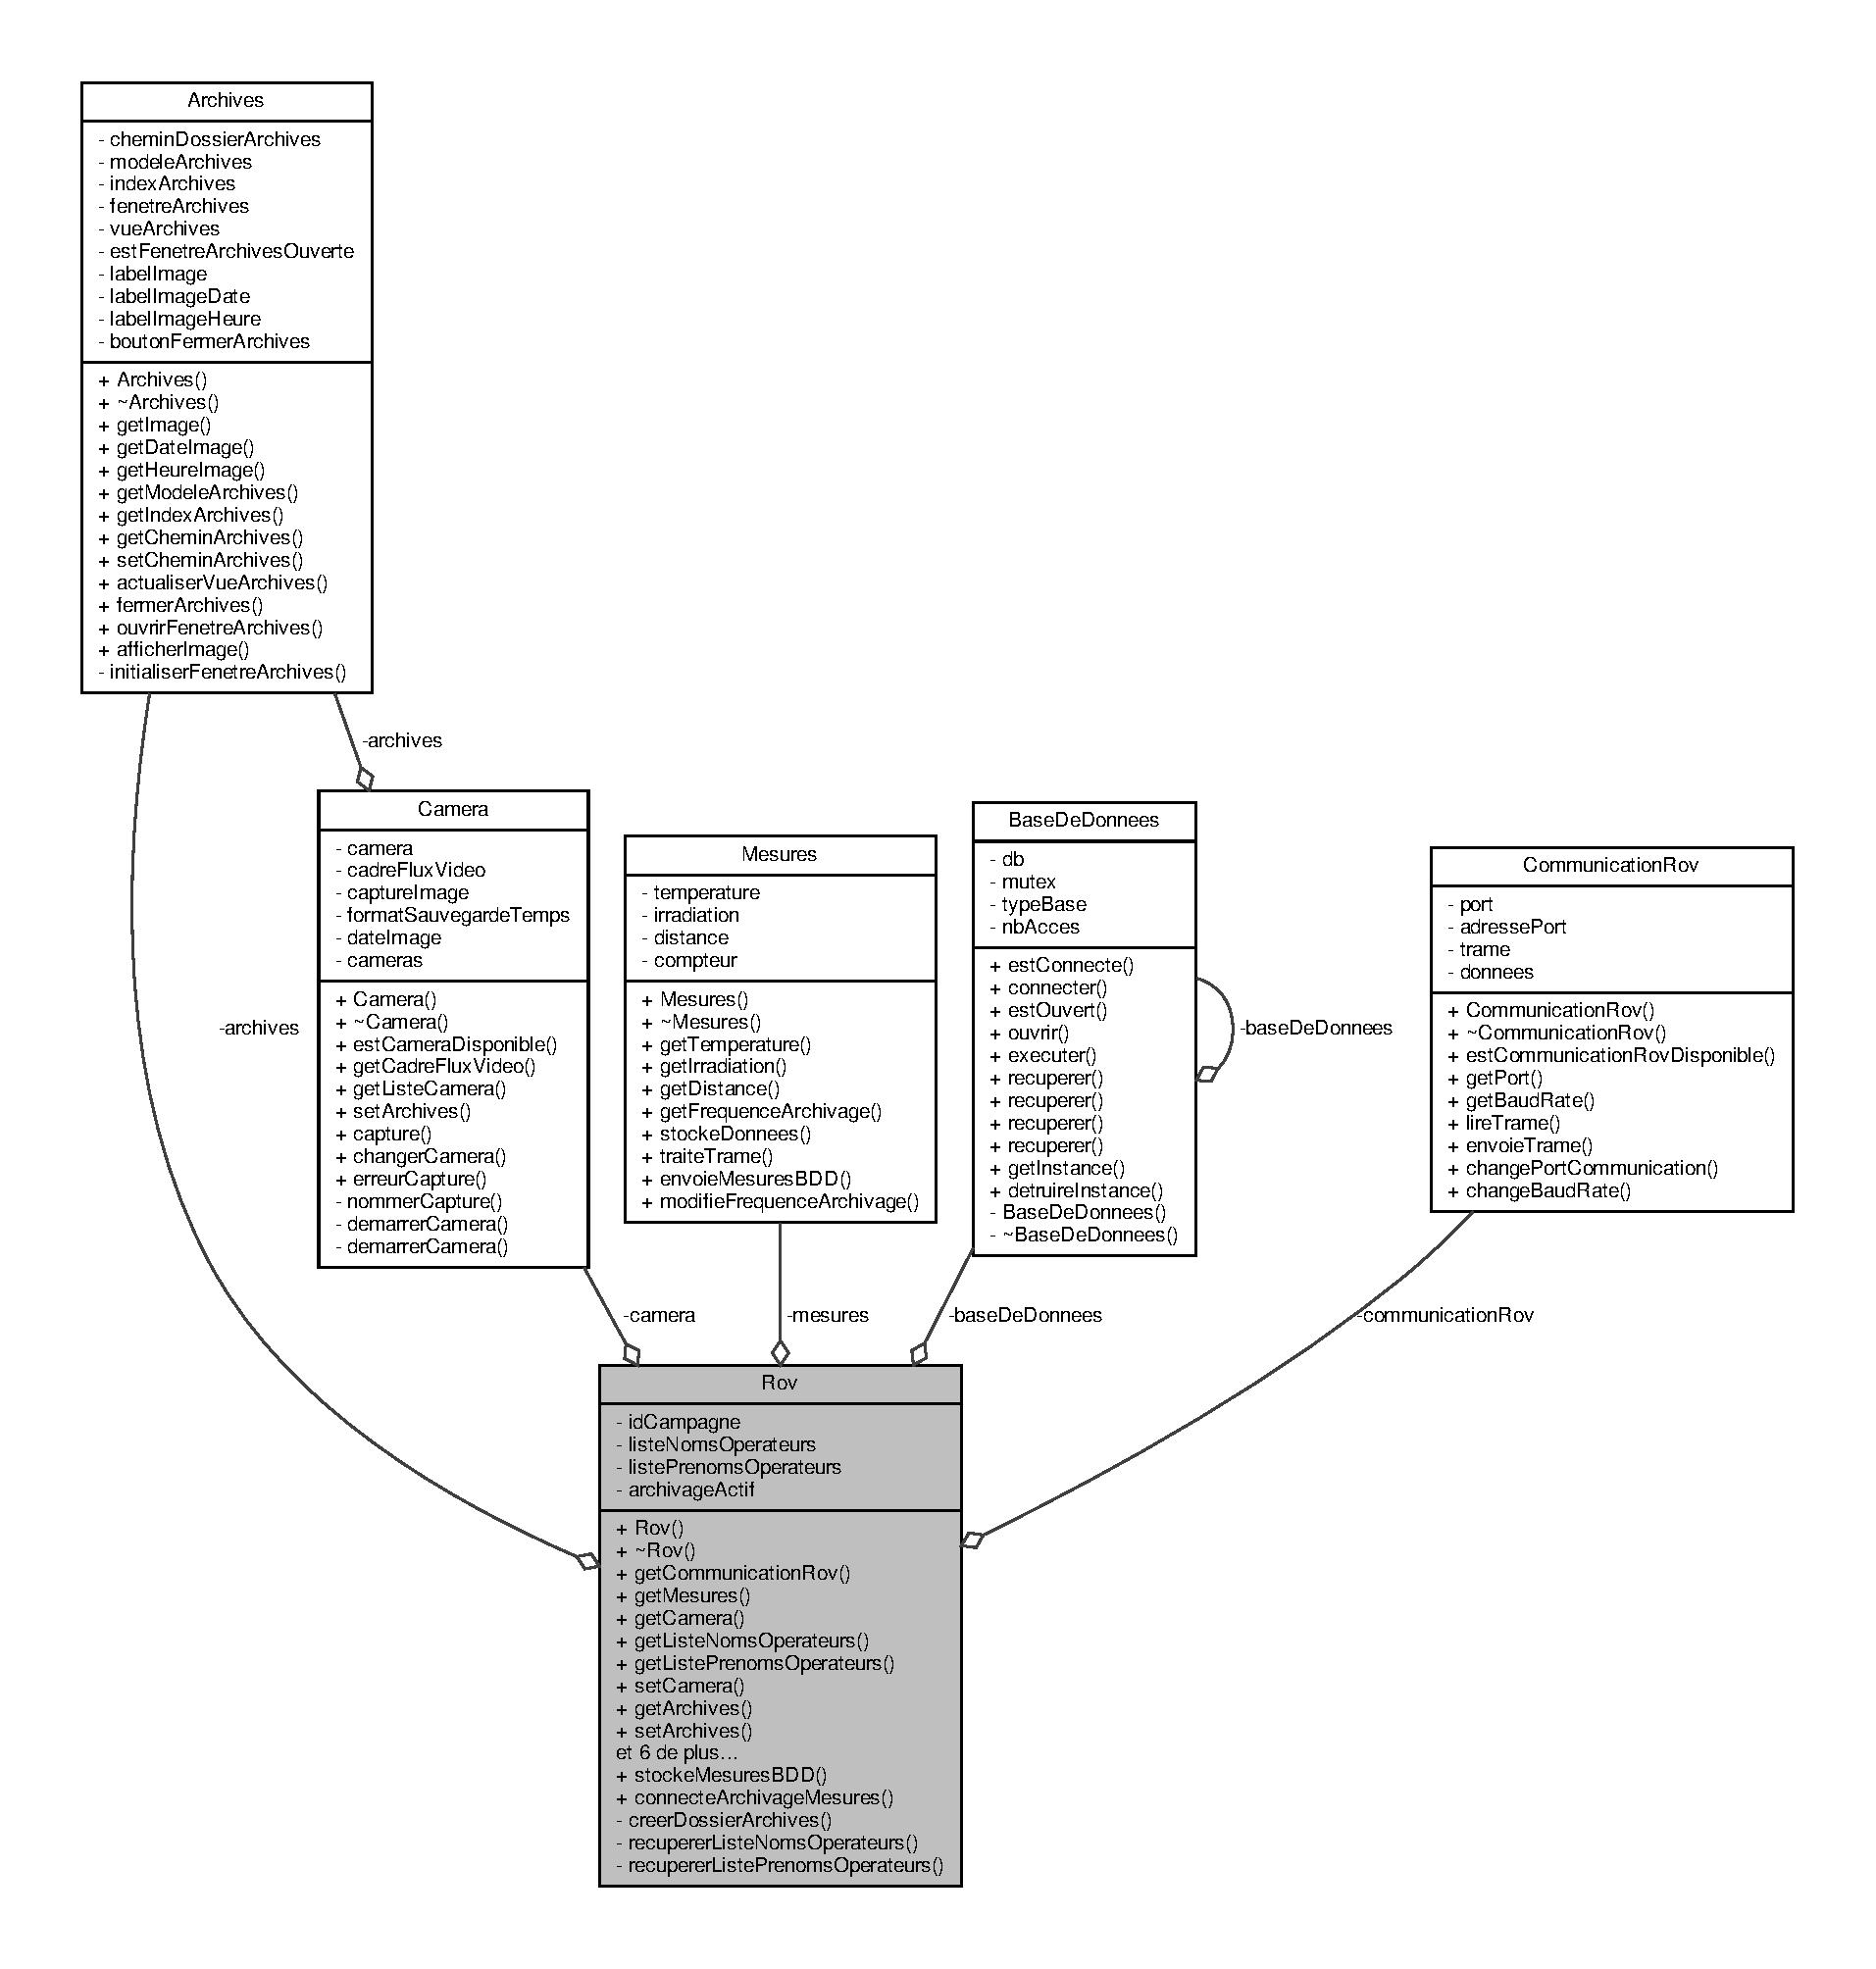
\includegraphics[width=350pt]{class_rov__coll__graph}
\end{center}
\end{figure}
\subsubsection*{Connecteurs publics}
\begin{DoxyCompactItemize}
\item 
void \hyperlink{class_rov_adab08abfde381c2915695489b34da6b4}{stocke\+Mesures\+B\+DD} (double temperature, double irradiation)
\begin{DoxyCompactList}\small\item\em Stocke les mesures dans la table mesures. \end{DoxyCompactList}\item 
void \hyperlink{class_rov_a738965ca84678b506b3d6a326c48e9e3}{connecte\+Archivage\+Mesures} (bool \hyperlink{class_rov_a659da5fe3636356b006a8e08a8433dd3}{archivage\+Actif})
\begin{DoxyCompactList}\small\item\em Active, ou désactive l\textquotesingle{}archivage des mesures dans la B\+DD. \end{DoxyCompactList}\end{DoxyCompactItemize}
\subsubsection*{Fonctions membres publiques}
\begin{DoxyCompactItemize}
\item 
\hyperlink{class_rov_a5dddd3bd156c134848078296087d090c}{Rov} (Q\+Object $\ast$parent=nullptr)
\begin{DoxyCompactList}\small\item\em Constructeur de la classe \hyperlink{class_rov}{Rov}. \end{DoxyCompactList}\item 
\hyperlink{class_rov_a6e41f712195b9af74fd75b781745d1b5}{$\sim$\+Rov} ()
\begin{DoxyCompactList}\small\item\em Destructeur de la classe \hyperlink{class_rov}{Rov}. \end{DoxyCompactList}\item 
\hyperlink{class_communication_rov}{Communication\+Rov} $\ast$ \hyperlink{class_rov_ad30543625f584e28bf785a80c59506dc}{get\+Communication\+Rov} () const
\begin{DoxyCompactList}\small\item\em Renvoie l\textquotesingle{}objet réalisant la connexion entre le rov et le programme. \end{DoxyCompactList}\item 
\hyperlink{class_mesures}{Mesures} $\ast$ \hyperlink{class_rov_a0edd5f7db785bd856b8723fe49ca7848}{get\+Mesures} () const
\begin{DoxyCompactList}\small\item\em Renvoie l\textquotesingle{}objet contenant les mesures et les méthodes affiliées. \end{DoxyCompactList}\item 
\hyperlink{class_camera}{Camera} $\ast$ \hyperlink{class_rov_aae07e8ca2c4b3be6a0a378b6f072c60b}{get\+Camera} () const
\begin{DoxyCompactList}\small\item\em Renvoie l\textquotesingle{}objet \hyperlink{class_camera}{Camera}. \end{DoxyCompactList}\item 
Q\+Vector$<$ Q\+String $>$ \hyperlink{class_rov_ab585cb1f82344ba0a64a28488910b262}{get\+Liste\+Noms\+Operateurs} ()
\begin{DoxyCompactList}\small\item\em Accesseur retournant la liste des noms des opérateurs. \end{DoxyCompactList}\item 
Q\+Vector$<$ Q\+String $>$ \hyperlink{class_rov_a128cae6dc19025017dea26663adde765}{get\+Liste\+Prenoms\+Operateurs} ()
\begin{DoxyCompactList}\small\item\em Accesseur retournant la liste des noms des opérateurs. \end{DoxyCompactList}\item 
void \hyperlink{class_rov_a0eba2119b89406948976ae92781c4629}{set\+Camera} (\hyperlink{class_camera}{Camera} $\ast$\hyperlink{class_rov_ad0461ecece812497ee9b4a962f168c18}{camera})
\begin{DoxyCompactList}\small\item\em Accesseur affectant une instance de la classe \hyperlink{class_camera}{Camera}. \end{DoxyCompactList}\item 
\hyperlink{class_archives}{Archives} $\ast$ \hyperlink{class_rov_af0936fd10d04851d53f28575ecd1da3f}{get\+Archives} () const
\begin{DoxyCompactList}\small\item\em Accesseur retournant une instance de la classe \hyperlink{class_archives}{Archives}. \end{DoxyCompactList}\item 
void \hyperlink{class_rov_acb3ecbb04ace455526206d3c05b712fd}{set\+Archives} (\hyperlink{class_archives}{Archives} $\ast$\hyperlink{class_rov_ad41ed46f169f28da226a979f70c4d8a4}{archives})
\begin{DoxyCompactList}\small\item\em Accesseur affectant une instance de la classe \hyperlink{class_archives}{Archives}. \end{DoxyCompactList}\item 
void \hyperlink{class_rov_a9bbaec4a59dae307440bfeefbc56190b}{set\+Id\+Campagne} (Q\+String \hyperlink{class_rov_aaaed58cd7ee9edbeab5251cd413a1bae}{id\+Campagne})
\begin{DoxyCompactList}\small\item\em Remplace l\textquotesingle{}id\+Campagne. \end{DoxyCompactList}\item 
Q\+String \hyperlink{class_rov_aaf98d93ef9b164a2e1766494d9577b57}{get\+Id\+Campagne} ()
\begin{DoxyCompactList}\small\item\em Renvoie id\+Campagne. \end{DoxyCompactList}\item 
bool \hyperlink{class_rov_ae1306036b067e9ad50a09f9dd607a092}{creer\+Nouvelle\+Campagne} (Q\+String nom, Q\+String description, Q\+String id\+Operateur)
\begin{DoxyCompactList}\small\item\em Crée une nouvelle campagne. \end{DoxyCompactList}\item 
bool \hyperlink{class_rov_a970f36e93f9dbd22734db571b21ceb04}{creer\+Dossiers\+Nouvelle\+Campagne} (Q\+String nom\+Nouvelle\+Campagne)
\begin{DoxyCompactList}\small\item\em Crée un dossier correspondant au nom de la campagne créée. \end{DoxyCompactList}\item 
void \hyperlink{class_rov_abbe2eb87a00b651c8259c0c7abca3edd}{set\+Archivage\+Actif} (bool)
\begin{DoxyCompactList}\small\item\em Modifie la valeur de archivage\+Actif. \end{DoxyCompactList}\item 
bool \hyperlink{class_rov_ac24b94eaac569252bdc0b1919489a761}{get\+Archivage\+Actif} () const
\begin{DoxyCompactList}\small\item\em Retourne l\textquotesingle{}état de archivage\+Actif. \end{DoxyCompactList}\end{DoxyCompactItemize}
\subsubsection*{Fonctions membres privées}
\begin{DoxyCompactItemize}
\item 
bool \hyperlink{class_rov_a53f656be57fa1eb7b93e03095a597439}{creer\+Dossier\+Archives} (Q\+String chemin\+Dossier\+Campagne)
\begin{DoxyCompactList}\small\item\em Crée le dossier des archives correspondant à la campagne créée. \end{DoxyCompactList}\item 
void \hyperlink{class_rov_a490eefb90bf28e83f181d770f0f52446}{recuperer\+Liste\+Noms\+Operateurs} ()
\begin{DoxyCompactList}\small\item\em Méthode permettant de récuperer la liste des noms opérateurs. \end{DoxyCompactList}\item 
void \hyperlink{class_rov_a84dece742f5c4c903ada4f25c869597f}{recuperer\+Liste\+Prenoms\+Operateurs} ()
\begin{DoxyCompactList}\small\item\em Méthode permettant de récuperer la liste des prenoms opérateurs. \end{DoxyCompactList}\end{DoxyCompactItemize}
\subsubsection*{Attributs privés}
\begin{DoxyCompactItemize}
\item 
\hyperlink{class_communication_rov}{Communication\+Rov} $\ast$ \hyperlink{class_rov_a8e7aaa17ee2134f26d57241d11ab2a99}{communication\+Rov}
\begin{DoxyCompactList}\small\item\em Communication via le port série avec le rov. \end{DoxyCompactList}\item 
\hyperlink{class_mesures}{Mesures} $\ast$ \hyperlink{class_rov_af37589b38493e4bd99702587db2d28a8}{mesures}
\begin{DoxyCompactList}\small\item\em Les mesures des capteurs. \end{DoxyCompactList}\item 
\hyperlink{class_camera}{Camera} $\ast$ \hyperlink{class_rov_ad0461ecece812497ee9b4a962f168c18}{camera}
\begin{DoxyCompactList}\small\item\em La caméra. \end{DoxyCompactList}\item 
\hyperlink{class_archives}{Archives} $\ast$ \hyperlink{class_rov_ad41ed46f169f28da226a979f70c4d8a4}{archives}
\begin{DoxyCompactList}\small\item\em Les archives. \end{DoxyCompactList}\item 
\hyperlink{class_base_de_donnees}{Base\+De\+Donnees} $\ast$ \hyperlink{class_rov_a5a9a824cd100947c75d0951eb9e1f90c}{base\+De\+Donnees}
\begin{DoxyCompactList}\small\item\em La base de données. \end{DoxyCompactList}\item 
Q\+String \hyperlink{class_rov_aaaed58cd7ee9edbeab5251cd413a1bae}{id\+Campagne}
\begin{DoxyCompactList}\small\item\em Numéro d\textquotesingle{}id de la campagne en cours. \end{DoxyCompactList}\item 
Q\+Vector$<$ Q\+String $>$ \hyperlink{class_rov_a3d424033e0ff00f480a711358ef4fde6}{liste\+Noms\+Operateurs}
\begin{DoxyCompactList}\small\item\em Liste des noms des opérateurs. \end{DoxyCompactList}\item 
Q\+Vector$<$ Q\+String $>$ \hyperlink{class_rov_a1e059749c13ed4ee9c0ec9168e79a3be}{liste\+Prenoms\+Operateurs}
\begin{DoxyCompactList}\small\item\em Liste des prenoms des opérateurs. \end{DoxyCompactList}\item 
bool \hyperlink{class_rov_a659da5fe3636356b006a8e08a8433dd3}{archivage\+Actif}
\begin{DoxyCompactList}\small\item\em L\textquotesingle{}archivage des mesures est demandé. \end{DoxyCompactList}\end{DoxyCompactItemize}


\subsubsection{Description détaillée}
\begin{DoxyAuthor}{Auteur}
R\+E\+Y\+N\+I\+ER Jacques \& Nicolas B\+O\+F\+F\+R\+E\+DO
\end{DoxyAuthor}
\begin{DoxyVersion}{Version}
1.\+1
\end{DoxyVersion}
\begin{DoxyDate}{Date}
Jeudi 13 Juin 2019 
\end{DoxyDate}


\subsubsection{Documentation des constructeurs et destructeur}
\mbox{\Hypertarget{class_rov_a5dddd3bd156c134848078296087d090c}\label{class_rov_a5dddd3bd156c134848078296087d090c}} 
\index{Rov@{Rov}!Rov@{Rov}}
\index{Rov@{Rov}!Rov@{Rov}}
\paragraph{\texorpdfstring{Rov()}{Rov()}}
{\footnotesize\ttfamily Rov\+::\+Rov (\begin{DoxyParamCaption}\item[{Q\+Object $\ast$}]{parent = {\ttfamily nullptr} }\end{DoxyParamCaption})\hspace{0.3cm}{\ttfamily [explicit]}}

Instancie des objets \hyperlink{class_archives}{Archives}, \hyperlink{class_communication_rov}{Communication\+Rov}, \hyperlink{class_mesures}{Mesures}, et \hyperlink{class_base_de_donnees}{Base\+De\+Donnees}. Se connecte à la B\+DD, et connecte les trames reçues à l\textquotesingle{}objet \hyperlink{class_mesures}{Mesures}.


\begin{DoxyParams}{Paramètres}
{\em parent} & \\
\hline
\end{DoxyParams}


Références \hyperlink{class_rov_a659da5fe3636356b006a8e08a8433dd3}{archivage\+Actif}, \hyperlink{class_rov_ad41ed46f169f28da226a979f70c4d8a4}{archives}, \hyperlink{class_rov_a5a9a824cd100947c75d0951eb9e1f90c}{base\+De\+Donnees}, \hyperlink{class_rov_a8e7aaa17ee2134f26d57241d11ab2a99}{communication\+Rov}, \hyperlink{class_rov_a738965ca84678b506b3d6a326c48e9e3}{connecte\+Archivage\+Mesures()}, \hyperlink{class_base_de_donnees_af9ac332082ffd0dd35e412cefabe5e9c}{Base\+De\+Donnees\+::est\+Ouvert()}, \hyperlink{class_base_de_donnees_a80028aa2b6b4fbf30fb2e36357b7d3d3}{Base\+De\+Donnees\+::get\+Instance()}, \hyperlink{class_rov_af37589b38493e4bd99702587db2d28a8}{mesures}, \hyperlink{class_base_de_donnees_a7f6a5510b08017b0d99115a84252f186}{Base\+De\+Donnees\+::ouvrir()}, \hyperlink{class_rov_a490eefb90bf28e83f181d770f0f52446}{recuperer\+Liste\+Noms\+Operateurs()}, et \hyperlink{class_rov_a84dece742f5c4c903ada4f25c869597f}{recuperer\+Liste\+Prenoms\+Operateurs()}.


\begin{DoxyCode}
00024                         : QObject(parent), \hyperlink{class_rov_a8e7aaa17ee2134f26d57241d11ab2a99}{communicationRov}(\textcolor{keyword}{nullptr}), 
      \hyperlink{class_rov_af37589b38493e4bd99702587db2d28a8}{mesures}(\textcolor{keyword}{nullptr}), \hyperlink{class_rov_ad0461ecece812497ee9b4a962f168c18}{camera}(\textcolor{keyword}{nullptr}), \hyperlink{class_rov_a3d424033e0ff00f480a711358ef4fde6}{listeNomsOperateurs}(0), 
      \hyperlink{class_rov_a1e059749c13ed4ee9c0ec9168e79a3be}{listePrenomsOperateurs}(0), \hyperlink{class_rov_a659da5fe3636356b006a8e08a8433dd3}{archivageActif}(1)
00025 \{
00026     qDebug() << Q\_FUNC\_INFO;
00027     \hyperlink{class_rov_ad41ed46f169f28da226a979f70c4d8a4}{archives} = \textcolor{keyword}{new} \hyperlink{class_archives}{Archives}(\textcolor{keyword}{this});
00028     \hyperlink{class_rov_a8e7aaa17ee2134f26d57241d11ab2a99}{communicationRov} = \textcolor{keyword}{new} \hyperlink{class_communication_rov}{CommunicationRov}(\textcolor{keyword}{this});
00029     \hyperlink{class_rov_af37589b38493e4bd99702587db2d28a8}{mesures} = \textcolor{keyword}{new} \hyperlink{class_mesures}{Mesures}(\textcolor{keyword}{this});
00030     \hyperlink{class_rov_a5a9a824cd100947c75d0951eb9e1f90c}{baseDeDonnees} = \hyperlink{class_base_de_donnees_a80028aa2b6b4fbf30fb2e36357b7d3d3}{BaseDeDonnees::getInstance}(\textcolor{stringliteral}{"QSQLITE"});
00031 
00032     \hyperlink{class_rov_a5a9a824cd100947c75d0951eb9e1f90c}{baseDeDonnees}->\hyperlink{class_base_de_donnees_a7f6a5510b08017b0d99115a84252f186}{ouvrir}(\textcolor{stringliteral}{"rovnet.sqlite"});
00033     \textcolor{keywordflow}{if}(\hyperlink{class_rov_a5a9a824cd100947c75d0951eb9e1f90c}{baseDeDonnees}->\hyperlink{class_base_de_donnees_af9ac332082ffd0dd35e412cefabe5e9c}{estOuvert}())
00034         qDebug() << Q\_FUNC\_INFO << \textcolor{stringliteral}{"ouverture réussie BD"};
00035     \textcolor{keywordflow}{else}
00036         qDebug() << Q\_FUNC\_INFO << \textcolor{stringliteral}{"echec ouverture BD"};
00037 
00038     \textcolor{comment}{// Connexions}
00039     connect(\hyperlink{class_rov_a8e7aaa17ee2134f26d57241d11ab2a99}{communicationRov}, SIGNAL(trameRecue(QString)), 
      \hyperlink{class_rov_af37589b38493e4bd99702587db2d28a8}{mesures}, SLOT(traiteTrame(QString)));
00040 
00041     \hyperlink{class_rov_a738965ca84678b506b3d6a326c48e9e3}{connecteArchivageMesures}(\hyperlink{class_rov_a659da5fe3636356b006a8e08a8433dd3}{archivageActif});
00042 
00043     \hyperlink{class_rov_a490eefb90bf28e83f181d770f0f52446}{recupererListeNomsOperateurs}();
00044     \hyperlink{class_rov_a84dece742f5c4c903ada4f25c869597f}{recupererListePrenomsOperateurs}();
00045 \}
\end{DoxyCode}
\mbox{\Hypertarget{class_rov_a6e41f712195b9af74fd75b781745d1b5}\label{class_rov_a6e41f712195b9af74fd75b781745d1b5}} 
\index{Rov@{Rov}!````~Rov@{$\sim$\+Rov}}
\index{````~Rov@{$\sim$\+Rov}!Rov@{Rov}}
\paragraph{\texorpdfstring{$\sim$\+Rov()}{~Rov()}}
{\footnotesize\ttfamily Rov\+::$\sim$\+Rov (\begin{DoxyParamCaption}{ }\end{DoxyParamCaption})}



Références \hyperlink{class_base_de_donnees_a457401c0816b888c77ce915997545f4e}{Base\+De\+Donnees\+::detruire\+Instance()}.


\begin{DoxyCode}
00052 \{
00053     \hyperlink{class_base_de_donnees_a457401c0816b888c77ce915997545f4e}{BaseDeDonnees::detruireInstance}();
00054     qDebug() << Q\_FUNC\_INFO;
00055 \}
\end{DoxyCode}


\subsubsection{Documentation des fonctions membres}
\mbox{\Hypertarget{class_rov_a738965ca84678b506b3d6a326c48e9e3}\label{class_rov_a738965ca84678b506b3d6a326c48e9e3}} 
\index{Rov@{Rov}!connecte\+Archivage\+Mesures@{connecte\+Archivage\+Mesures}}
\index{connecte\+Archivage\+Mesures@{connecte\+Archivage\+Mesures}!Rov@{Rov}}
\paragraph{\texorpdfstring{connecte\+Archivage\+Mesures}{connecteArchivageMesures}}
{\footnotesize\ttfamily void Rov\+::connecte\+Archivage\+Mesures (\begin{DoxyParamCaption}\item[{bool}]{archivage\+Actif }\end{DoxyParamCaption})\hspace{0.3cm}{\ttfamily [slot]}}

Active ou désactive l\textquotesingle{}archivage des mesures dans la B\+DD.


\begin{DoxyParams}{Paramètres}
{\em archivage\+Actif} & bool nouvel état d\textquotesingle{}activation. \\
\hline
\end{DoxyParams}


Références \hyperlink{class_rov_af37589b38493e4bd99702587db2d28a8}{mesures}, et \hyperlink{class_rov_adab08abfde381c2915695489b34da6b4}{stocke\+Mesures\+B\+D\+D()}.



Référencé par \hyperlink{class_rov_a5dddd3bd156c134848078296087d090c}{Rov()}, et \hyperlink{class_rov_abbe2eb87a00b651c8259c0c7abca3edd}{set\+Archivage\+Actif()}.


\begin{DoxyCode}
00085 \{
00086     \textcolor{keywordflow}{if}(\hyperlink{class_rov_a659da5fe3636356b006a8e08a8433dd3}{archivageActif})
00087         connect(\hyperlink{class_rov_af37589b38493e4bd99702587db2d28a8}{mesures}, SIGNAL(mesuresBDDPrete(\textcolor{keywordtype}{double}, \textcolor{keywordtype}{double})), \textcolor{keyword}{this}, SLOT(
      \hyperlink{class_rov_adab08abfde381c2915695489b34da6b4}{stockeMesuresBDD}(\textcolor{keywordtype}{double}, \textcolor{keywordtype}{double})));
00088     \textcolor{keywordflow}{else}
00089         disconnect(\hyperlink{class_rov_af37589b38493e4bd99702587db2d28a8}{mesures}, SIGNAL(mesuresBDDPrete(\textcolor{keywordtype}{double}, \textcolor{keywordtype}{double})), \textcolor{keyword}{this}, SLOT(
      \hyperlink{class_rov_adab08abfde381c2915695489b34da6b4}{stockeMesuresBDD}(\textcolor{keywordtype}{double}, \textcolor{keywordtype}{double})));
00090 \}
\end{DoxyCode}
\mbox{\Hypertarget{class_rov_a53f656be57fa1eb7b93e03095a597439}\label{class_rov_a53f656be57fa1eb7b93e03095a597439}} 
\index{Rov@{Rov}!creer\+Dossier\+Archives@{creer\+Dossier\+Archives}}
\index{creer\+Dossier\+Archives@{creer\+Dossier\+Archives}!Rov@{Rov}}
\paragraph{\texorpdfstring{creer\+Dossier\+Archives()}{creerDossierArchives()}}
{\footnotesize\ttfamily bool Rov\+::creer\+Dossier\+Archives (\begin{DoxyParamCaption}\item[{Q\+String}]{chemin\+Dossier\+Campagne }\end{DoxyParamCaption})\hspace{0.3cm}{\ttfamily [private]}}



Références \hyperlink{class_rov_ad41ed46f169f28da226a979f70c4d8a4}{archives}, et \hyperlink{class_archives_a899e95a34c2a6f79b9a25355b5bf9cb6}{Archives\+::set\+Chemin\+Archives()}.



Référencé par \hyperlink{class_rov_a970f36e93f9dbd22734db571b21ceb04}{creer\+Dossiers\+Nouvelle\+Campagne()}.


\begin{DoxyCode}
00247 \{
00248     qDebug() << Q\_FUNC\_INFO;
00249     QDir dossierArchives(cheminDossierCampagne);
00250     \textcolor{keywordflow}{if}(dossierArchives.mkdir(\textcolor{stringliteral}{"Archives"}))
00251     \{
00252         QString cheminDossierArchives = cheminDossierCampagne + \textcolor{stringliteral}{"/Archives/"};
00253         qDebug() << Q\_FUNC\_INFO << \hyperlink{class_rov_ad41ed46f169f28da226a979f70c4d8a4}{archives} << cheminDossierArchives;
00254         \hyperlink{class_rov_ad41ed46f169f28da226a979f70c4d8a4}{archives}->\hyperlink{class_archives_a899e95a34c2a6f79b9a25355b5bf9cb6}{setCheminArchives}(cheminDossierArchives);
00255         \textcolor{keywordflow}{return} \textcolor{keyword}{true};
00256     \}
00257     \textcolor{keywordflow}{return} \textcolor{keyword}{false};
00258 \}
\end{DoxyCode}
\mbox{\Hypertarget{class_rov_a970f36e93f9dbd22734db571b21ceb04}\label{class_rov_a970f36e93f9dbd22734db571b21ceb04}} 
\index{Rov@{Rov}!creer\+Dossiers\+Nouvelle\+Campagne@{creer\+Dossiers\+Nouvelle\+Campagne}}
\index{creer\+Dossiers\+Nouvelle\+Campagne@{creer\+Dossiers\+Nouvelle\+Campagne}!Rov@{Rov}}
\paragraph{\texorpdfstring{creer\+Dossiers\+Nouvelle\+Campagne()}{creerDossiersNouvelleCampagne()}}
{\footnotesize\ttfamily bool Rov\+::creer\+Dossiers\+Nouvelle\+Campagne (\begin{DoxyParamCaption}\item[{Q\+String}]{nom\+Nouvelle\+Campagne }\end{DoxyParamCaption})}



Références \hyperlink{class_rov_a53f656be57fa1eb7b93e03095a597439}{creer\+Dossier\+Archives()}.



Référencé par \hyperlink{class_rov_ae1306036b067e9ad50a09f9dd607a092}{creer\+Nouvelle\+Campagne()}.


\begin{DoxyCode}
00231 \{
00232     QDir dossierApplication(QApplication::applicationDirPath());
00233     \textcolor{keywordflow}{if}(dossierApplication.mkdir(nomNouvelleCampagne))
00234     \{
00235         QString cheminDossierCampagne = QApplication::applicationDirPath() + \textcolor{stringliteral}{"/"} + nomNouvelleCampagne;
00236         qDebug() << Q\_FUNC\_INFO << cheminDossierCampagne;
00237         \textcolor{keywordflow}{return} \hyperlink{class_rov_a53f656be57fa1eb7b93e03095a597439}{creerDossierArchives}(cheminDossierCampagne);
00238     \}
00239     \textcolor{keywordflow}{return} \textcolor{keyword}{false};
00240 \}
\end{DoxyCode}
\mbox{\Hypertarget{class_rov_ae1306036b067e9ad50a09f9dd607a092}\label{class_rov_ae1306036b067e9ad50a09f9dd607a092}} 
\index{Rov@{Rov}!creer\+Nouvelle\+Campagne@{creer\+Nouvelle\+Campagne}}
\index{creer\+Nouvelle\+Campagne@{creer\+Nouvelle\+Campagne}!Rov@{Rov}}
\paragraph{\texorpdfstring{creer\+Nouvelle\+Campagne()}{creerNouvelleCampagne()}}
{\footnotesize\ttfamily bool Rov\+::creer\+Nouvelle\+Campagne (\begin{DoxyParamCaption}\item[{Q\+String}]{nom,  }\item[{Q\+String}]{description,  }\item[{Q\+String}]{id\+Operateur }\end{DoxyParamCaption})}


\begin{DoxyParams}{Paramètres}
{\em nom} & Q\+String \\
\hline
{\em description} & Q\+String \\
\hline
{\em id\+Operateur} & Q\+String \\
\hline
\end{DoxyParams}
\begin{DoxyReturn}{Renvoie}
bool 
\end{DoxyReturn}


Références \hyperlink{class_rov_ad41ed46f169f28da226a979f70c4d8a4}{archives}, \hyperlink{class_rov_a5a9a824cd100947c75d0951eb9e1f90c}{base\+De\+Donnees}, \hyperlink{class_rov_a8e7aaa17ee2134f26d57241d11ab2a99}{communication\+Rov}, \hyperlink{class_rov_a970f36e93f9dbd22734db571b21ceb04}{creer\+Dossiers\+Nouvelle\+Campagne()}, \hyperlink{class_communication_rov_a513c26b04745fa2ae31b4533d656dfd4}{Communication\+Rov\+::est\+Communication\+Rov\+Disponible()}, \hyperlink{class_base_de_donnees_aa8de5f8f8bb17edc43f5c0ee33712081}{Base\+De\+Donnees\+::executer()}, \hyperlink{class_archives_a65dfbaba0123e6530b03bfb70e614c90}{Archives\+::get\+Chemin\+Archives()}, \hyperlink{class_rov_aaaed58cd7ee9edbeab5251cd413a1bae}{id\+Campagne}, \hyperlink{class_base_de_donnees_a77539baad389f5acf754cd2cd452403e}{Base\+De\+Donnees\+::recuperer()}, et \hyperlink{class_rov_a9bbaec4a59dae307440bfeefbc56190b}{set\+Id\+Campagne()}.



Référencé par \hyperlink{class_i_h_m_rov_a229194814bfb1fc94ab3cc86d6411921}{I\+H\+M\+Rov\+::enregistrer\+Parametres\+Campagne()}.


\begin{DoxyCode}
00178 \{
00179     \textcolor{keywordflow}{if}(\hyperlink{class_rov_a8e7aaa17ee2134f26d57241d11ab2a99}{communicationRov}->\hyperlink{class_communication_rov_a513c26b04745fa2ae31b4533d656dfd4}{estCommunicationRovDisponible}())
00180     \{
00181         \textcolor{keywordflow}{if}(\hyperlink{class_rov_a970f36e93f9dbd22734db571b21ceb04}{creerDossiersNouvelleCampagne}(nom))
00182         \{
00183             QString cheminArchives = \hyperlink{class_rov_ad41ed46f169f28da226a979f70c4d8a4}{archives}->\hyperlink{class_archives_a65dfbaba0123e6530b03bfb70e614c90}{getCheminArchives}();
00184             QString requete = \textcolor{stringliteral}{"INSERT INTO 'campagnes'(nom, description, date, cheminArchives, idOperateur)
       VALUES ('"} + nom + \textcolor{stringliteral}{"', '"} + description + \textcolor{stringliteral}{"', datetime('now', 'localtime'), '"} + cheminArchives + \textcolor{stringliteral}{"', '"} + 
      idOperateur + \textcolor{stringliteral}{"')"};
00185             \textcolor{keywordtype}{bool} retour = \hyperlink{class_rov_a5a9a824cd100947c75d0951eb9e1f90c}{baseDeDonnees}->\hyperlink{class_base_de_donnees_aa8de5f8f8bb17edc43f5c0ee33712081}{executer}(requete);
00186             \textcolor{keywordflow}{if}(!retour)
00187             \{
00188                 \textcolor{keywordflow}{return} \textcolor{keyword}{false};
00189             \}
00190 
00191             QString \hyperlink{class_rov_aaaed58cd7ee9edbeab5251cd413a1bae}{idCampagne};
00192             \textcolor{keywordtype}{bool} requeteRecupIdCampagne = \hyperlink{class_rov_a5a9a824cd100947c75d0951eb9e1f90c}{baseDeDonnees}->\hyperlink{class_base_de_donnees_a77539baad389f5acf754cd2cd452403e}{recuperer}(\textcolor{stringliteral}{"SELECT idCampagne
       FROM campagnes WHERE cheminArchives = '"} + cheminArchives + \textcolor{stringliteral}{"';"}, idCampagne);
00193             \textcolor{keywordflow}{if}(requeteRecupIdCampagne)
00194             \{
00195                 \hyperlink{class_rov_a9bbaec4a59dae307440bfeefbc56190b}{setIdCampagne}(idCampagne);
00196             \}
00197             \textcolor{keywordflow}{else}
00198             \{
00199                 \textcolor{keywordflow}{return} \textcolor{keyword}{false};
00200             \}
00201             \textcolor{keywordflow}{return} \textcolor{keyword}{true};
00202         \}
00203         \textcolor{keywordflow}{else}
00204             \textcolor{keywordflow}{return} \textcolor{keyword}{false};
00205     \}
00206     \textcolor{keywordflow}{else}
00207         \textcolor{keywordflow}{return} \textcolor{keyword}{false};
00208 \}
\end{DoxyCode}
\mbox{\Hypertarget{class_rov_ac24b94eaac569252bdc0b1919489a761}\label{class_rov_ac24b94eaac569252bdc0b1919489a761}} 
\index{Rov@{Rov}!get\+Archivage\+Actif@{get\+Archivage\+Actif}}
\index{get\+Archivage\+Actif@{get\+Archivage\+Actif}!Rov@{Rov}}
\paragraph{\texorpdfstring{get\+Archivage\+Actif()}{getArchivageActif()}}
{\footnotesize\ttfamily bool Rov\+::get\+Archivage\+Actif (\begin{DoxyParamCaption}{ }\end{DoxyParamCaption}) const}

Indique si l\textquotesingle{}archivage des mesures dans la B\+DD est activé ou non.

\begin{DoxyReturn}{Renvoie}
bool archivage\+Actif état d\textquotesingle{}activation de l\textquotesingle{}archivage des mesures. 
\end{DoxyReturn}


Références \hyperlink{class_rov_a659da5fe3636356b006a8e08a8433dd3}{archivage\+Actif}.


\begin{DoxyCode}
00075 \{
00076     \textcolor{keywordflow}{return} this->\hyperlink{class_rov_a659da5fe3636356b006a8e08a8433dd3}{archivageActif};
00077 \}
\end{DoxyCode}
\mbox{\Hypertarget{class_rov_af0936fd10d04851d53f28575ecd1da3f}\label{class_rov_af0936fd10d04851d53f28575ecd1da3f}} 
\index{Rov@{Rov}!get\+Archives@{get\+Archives}}
\index{get\+Archives@{get\+Archives}!Rov@{Rov}}
\paragraph{\texorpdfstring{get\+Archives()}{getArchives()}}
{\footnotesize\ttfamily \hyperlink{class_archives}{Archives} $\ast$ Rov\+::get\+Archives (\begin{DoxyParamCaption}{ }\end{DoxyParamCaption}) const}

\begin{DoxyReturn}{Renvoie}
une instance de la classe {\itshape \hyperlink{class_archives}{Archives}} 
\end{DoxyReturn}


Références \hyperlink{class_rov_ad41ed46f169f28da226a979f70c4d8a4}{archives}.


\begin{DoxyCode}
00128 \{
00129     \textcolor{keywordflow}{return} \hyperlink{class_rov_ad41ed46f169f28da226a979f70c4d8a4}{archives};
00130 \}
\end{DoxyCode}
\mbox{\Hypertarget{class_rov_aae07e8ca2c4b3be6a0a378b6f072c60b}\label{class_rov_aae07e8ca2c4b3be6a0a378b6f072c60b}} 
\index{Rov@{Rov}!get\+Camera@{get\+Camera}}
\index{get\+Camera@{get\+Camera}!Rov@{Rov}}
\paragraph{\texorpdfstring{get\+Camera()}{getCamera()}}
{\footnotesize\ttfamily \hyperlink{class_camera}{Camera} $\ast$ Rov\+::get\+Camera (\begin{DoxyParamCaption}{ }\end{DoxyParamCaption}) const}

Accesseur retournant une instance de la classe \hyperlink{class_camera}{Camera}.

\begin{DoxyReturn}{Renvoie}
une instance de la classe {\itshape \hyperlink{class_camera}{Camera}} 
\end{DoxyReturn}


Références \hyperlink{class_rov_ad0461ecece812497ee9b4a962f168c18}{camera}.


\begin{DoxyCode}
00118 \{
00119     \textcolor{keywordflow}{return} \hyperlink{class_rov_ad0461ecece812497ee9b4a962f168c18}{camera};
00120 \}
\end{DoxyCode}
\mbox{\Hypertarget{class_rov_ad30543625f584e28bf785a80c59506dc}\label{class_rov_ad30543625f584e28bf785a80c59506dc}} 
\index{Rov@{Rov}!get\+Communication\+Rov@{get\+Communication\+Rov}}
\index{get\+Communication\+Rov@{get\+Communication\+Rov}!Rov@{Rov}}
\paragraph{\texorpdfstring{get\+Communication\+Rov()}{getCommunicationRov()}}
{\footnotesize\ttfamily \hyperlink{class_communication_rov}{Communication\+Rov} $\ast$ Rov\+::get\+Communication\+Rov (\begin{DoxyParamCaption}{ }\end{DoxyParamCaption}) const}

Accesseur retournant une instance de la classe \hyperlink{class_communication_rov}{Communication\+Rov}.

\begin{DoxyReturn}{Renvoie}
une instance de la classe {\itshape \hyperlink{class_communication_rov}{Communication\+Rov}} 
\end{DoxyReturn}


Références \hyperlink{class_rov_a8e7aaa17ee2134f26d57241d11ab2a99}{communication\+Rov}.



Référencé par \hyperlink{class_i_h_m_rov_abbfcdc154a6ae7f941d186f6c90a5a2b}{I\+H\+M\+Rov\+::actualise\+Icones\+Etat()}, \hyperlink{class_controle_rov_acc4d5fea26770217df978d43df2ad51e}{Controle\+Rov\+::\+Controle\+Rov()}, \hyperlink{class_i_h_m_rov_aed451139ac09ef18b7c92637761d80ce}{I\+H\+M\+Rov\+::creer\+Fenetre\+Parametres()}, et \hyperlink{class_i_h_m_rov_a94d31f4e748f3e4549eab42c8bc7e367}{I\+H\+M\+Rov\+::enregistrer\+Parametres()}.


\begin{DoxyCode}
00098 \{
00099     \textcolor{keywordflow}{return} this->\hyperlink{class_rov_a8e7aaa17ee2134f26d57241d11ab2a99}{communicationRov};
00100 \}
\end{DoxyCode}
\mbox{\Hypertarget{class_rov_aaf98d93ef9b164a2e1766494d9577b57}\label{class_rov_aaf98d93ef9b164a2e1766494d9577b57}} 
\index{Rov@{Rov}!get\+Id\+Campagne@{get\+Id\+Campagne}}
\index{get\+Id\+Campagne@{get\+Id\+Campagne}!Rov@{Rov}}
\paragraph{\texorpdfstring{get\+Id\+Campagne()}{getIdCampagne()}}
{\footnotesize\ttfamily Q\+String Rov\+::get\+Id\+Campagne (\begin{DoxyParamCaption}{ }\end{DoxyParamCaption})}

Accesseur retournant l\textquotesingle{}id de la campagne en cours.

\begin{DoxyReturn}{Renvoie}
un {\itshape Q\+String} correspondant à l\textquotesingle{}id de la campagne en cours. 
\end{DoxyReturn}


Références \hyperlink{class_rov_aaaed58cd7ee9edbeab5251cd413a1bae}{id\+Campagne}.


\begin{DoxyCode}
00165 \{
00166     \textcolor{keywordflow}{return} this->\hyperlink{class_rov_aaaed58cd7ee9edbeab5251cd413a1bae}{idCampagne};
00167 \}
\end{DoxyCode}
\mbox{\Hypertarget{class_rov_ab585cb1f82344ba0a64a28488910b262}\label{class_rov_ab585cb1f82344ba0a64a28488910b262}} 
\index{Rov@{Rov}!get\+Liste\+Noms\+Operateurs@{get\+Liste\+Noms\+Operateurs}}
\index{get\+Liste\+Noms\+Operateurs@{get\+Liste\+Noms\+Operateurs}!Rov@{Rov}}
\paragraph{\texorpdfstring{get\+Liste\+Noms\+Operateurs()}{getListeNomsOperateurs()}}
{\footnotesize\ttfamily Q\+Vector$<$ Q\+String $>$ Rov\+::get\+Liste\+Noms\+Operateurs (\begin{DoxyParamCaption}{ }\end{DoxyParamCaption})}

\begin{DoxyReturn}{Renvoie}
un {\itshape Q\+Vector} de {\itshape Q\+String}, la liste des noms des opérateurs 
\end{DoxyReturn}


Références \hyperlink{class_rov_a3d424033e0ff00f480a711358ef4fde6}{liste\+Noms\+Operateurs}.



Référencé par \hyperlink{class_i_h_m_rov_a752a8dc2b3b68d536e94ff8bfb62f46f}{I\+H\+M\+Rov\+::remplir\+Combo\+Box\+Liste\+Operateurs()}.


\begin{DoxyCode}
00283 \{
00284     \textcolor{keywordflow}{return} \hyperlink{class_rov_a3d424033e0ff00f480a711358ef4fde6}{listeNomsOperateurs};
00285 \}
\end{DoxyCode}
\mbox{\Hypertarget{class_rov_a128cae6dc19025017dea26663adde765}\label{class_rov_a128cae6dc19025017dea26663adde765}} 
\index{Rov@{Rov}!get\+Liste\+Prenoms\+Operateurs@{get\+Liste\+Prenoms\+Operateurs}}
\index{get\+Liste\+Prenoms\+Operateurs@{get\+Liste\+Prenoms\+Operateurs}!Rov@{Rov}}
\paragraph{\texorpdfstring{get\+Liste\+Prenoms\+Operateurs()}{getListePrenomsOperateurs()}}
{\footnotesize\ttfamily Q\+Vector$<$ Q\+String $>$ Rov\+::get\+Liste\+Prenoms\+Operateurs (\begin{DoxyParamCaption}{ }\end{DoxyParamCaption})}

\begin{DoxyReturn}{Renvoie}
un {\itshape Q\+Vector} de {\itshape Q\+String}, la liste des noms des opérateurs 
\end{DoxyReturn}


Références \hyperlink{class_rov_a1e059749c13ed4ee9c0ec9168e79a3be}{liste\+Prenoms\+Operateurs}.



Référencé par \hyperlink{class_i_h_m_rov_a752a8dc2b3b68d536e94ff8bfb62f46f}{I\+H\+M\+Rov\+::remplir\+Combo\+Box\+Liste\+Operateurs()}.


\begin{DoxyCode}
00310 \{
00311     \textcolor{keywordflow}{return} \hyperlink{class_rov_a1e059749c13ed4ee9c0ec9168e79a3be}{listePrenomsOperateurs};
00312 \}
\end{DoxyCode}
\mbox{\Hypertarget{class_rov_a0edd5f7db785bd856b8723fe49ca7848}\label{class_rov_a0edd5f7db785bd856b8723fe49ca7848}} 
\index{Rov@{Rov}!get\+Mesures@{get\+Mesures}}
\index{get\+Mesures@{get\+Mesures}!Rov@{Rov}}
\paragraph{\texorpdfstring{get\+Mesures()}{getMesures()}}
{\footnotesize\ttfamily \hyperlink{class_mesures}{Mesures} $\ast$ Rov\+::get\+Mesures (\begin{DoxyParamCaption}{ }\end{DoxyParamCaption}) const}

Accesseur retournant une instance de la classe \hyperlink{class_mesures}{Mesures}.

\begin{DoxyReturn}{Renvoie}
une instance de la classe {\itshape \hyperlink{class_mesures}{Mesures}} 
\end{DoxyReturn}


Références \hyperlink{class_rov_af37589b38493e4bd99702587db2d28a8}{mesures}.



Référencé par \hyperlink{class_i_h_m_rov_aed451139ac09ef18b7c92637761d80ce}{I\+H\+M\+Rov\+::creer\+Fenetre\+Parametres()}, et \hyperlink{class_i_h_m_rov_a5dac1fb4612866cc61f699a415e0ef6b}{I\+H\+M\+Rov\+::\+I\+H\+M\+Rov()}.


\begin{DoxyCode}
00108 \{
00109     \textcolor{keywordflow}{return} \hyperlink{class_rov_af37589b38493e4bd99702587db2d28a8}{mesures};
00110 \}
\end{DoxyCode}
\mbox{\Hypertarget{class_rov_a490eefb90bf28e83f181d770f0f52446}\label{class_rov_a490eefb90bf28e83f181d770f0f52446}} 
\index{Rov@{Rov}!recuperer\+Liste\+Noms\+Operateurs@{recuperer\+Liste\+Noms\+Operateurs}}
\index{recuperer\+Liste\+Noms\+Operateurs@{recuperer\+Liste\+Noms\+Operateurs}!Rov@{Rov}}
\paragraph{\texorpdfstring{recuperer\+Liste\+Noms\+Operateurs()}{recupererListeNomsOperateurs()}}
{\footnotesize\ttfamily void Rov\+::recuperer\+Liste\+Noms\+Operateurs (\begin{DoxyParamCaption}{ }\end{DoxyParamCaption})\hspace{0.3cm}{\ttfamily [private]}}



Références \hyperlink{class_rov_a5a9a824cd100947c75d0951eb9e1f90c}{base\+De\+Donnees}, \hyperlink{class_rov_a3d424033e0ff00f480a711358ef4fde6}{liste\+Noms\+Operateurs}, et \hyperlink{class_base_de_donnees_a77539baad389f5acf754cd2cd452403e}{Base\+De\+Donnees\+::recuperer()}.



Référencé par \hyperlink{class_rov_a5dddd3bd156c134848078296087d090c}{Rov()}.


\begin{DoxyCode}
00265 \{
00266     QString requete = \textcolor{stringliteral}{"SELECT nom FROM operateurs"};
00267     \textcolor{keywordtype}{bool} reussi = \hyperlink{class_rov_a5a9a824cd100947c75d0951eb9e1f90c}{baseDeDonnees}->\hyperlink{class_base_de_donnees_a77539baad389f5acf754cd2cd452403e}{recuperer}(requete, 
      \hyperlink{class_rov_a3d424033e0ff00f480a711358ef4fde6}{listeNomsOperateurs});
00268     qDebug() << requete << \hyperlink{class_rov_a3d424033e0ff00f480a711358ef4fde6}{listeNomsOperateurs};
00269 
00270     \textcolor{keywordflow}{if}(reussi)
00271         qDebug() << Q\_FUNC\_INFO << \hyperlink{class_rov_a3d424033e0ff00f480a711358ef4fde6}{listeNomsOperateurs};
00272 
00273     \textcolor{keywordflow}{else}
00274         qDebug() << Q\_FUNC\_INFO << \textcolor{stringliteral}{"erreur SQL"} << requete;
00275 \}
\end{DoxyCode}
\mbox{\Hypertarget{class_rov_a84dece742f5c4c903ada4f25c869597f}\label{class_rov_a84dece742f5c4c903ada4f25c869597f}} 
\index{Rov@{Rov}!recuperer\+Liste\+Prenoms\+Operateurs@{recuperer\+Liste\+Prenoms\+Operateurs}}
\index{recuperer\+Liste\+Prenoms\+Operateurs@{recuperer\+Liste\+Prenoms\+Operateurs}!Rov@{Rov}}
\paragraph{\texorpdfstring{recuperer\+Liste\+Prenoms\+Operateurs()}{recupererListePrenomsOperateurs()}}
{\footnotesize\ttfamily void Rov\+::recuperer\+Liste\+Prenoms\+Operateurs (\begin{DoxyParamCaption}{ }\end{DoxyParamCaption})\hspace{0.3cm}{\ttfamily [private]}}



Références \hyperlink{class_rov_a5a9a824cd100947c75d0951eb9e1f90c}{base\+De\+Donnees}, \hyperlink{class_rov_a1e059749c13ed4ee9c0ec9168e79a3be}{liste\+Prenoms\+Operateurs}, et \hyperlink{class_base_de_donnees_a77539baad389f5acf754cd2cd452403e}{Base\+De\+Donnees\+::recuperer()}.



Référencé par \hyperlink{class_rov_a5dddd3bd156c134848078296087d090c}{Rov()}.


\begin{DoxyCode}
00292 \{
00293     QString requete = \textcolor{stringliteral}{"SELECT prenom FROM operateurs"};
00294     \textcolor{keywordtype}{bool} reussi = \hyperlink{class_rov_a5a9a824cd100947c75d0951eb9e1f90c}{baseDeDonnees}->\hyperlink{class_base_de_donnees_a77539baad389f5acf754cd2cd452403e}{recuperer}(requete, 
      \hyperlink{class_rov_a1e059749c13ed4ee9c0ec9168e79a3be}{listePrenomsOperateurs});
00295     qDebug() << requete << \hyperlink{class_rov_a1e059749c13ed4ee9c0ec9168e79a3be}{listePrenomsOperateurs};
00296 
00297     \textcolor{keywordflow}{if}(reussi)
00298         qDebug() << Q\_FUNC\_INFO << \hyperlink{class_rov_a1e059749c13ed4ee9c0ec9168e79a3be}{listePrenomsOperateurs};
00299 
00300     \textcolor{keywordflow}{else}
00301         qDebug() << Q\_FUNC\_INFO << \textcolor{stringliteral}{"erreur SQL"} << requete;
00302 \}
\end{DoxyCode}
\mbox{\Hypertarget{class_rov_abbe2eb87a00b651c8259c0c7abca3edd}\label{class_rov_abbe2eb87a00b651c8259c0c7abca3edd}} 
\index{Rov@{Rov}!set\+Archivage\+Actif@{set\+Archivage\+Actif}}
\index{set\+Archivage\+Actif@{set\+Archivage\+Actif}!Rov@{Rov}}
\paragraph{\texorpdfstring{set\+Archivage\+Actif()}{setArchivageActif()}}
{\footnotesize\ttfamily void Rov\+::set\+Archivage\+Actif (\begin{DoxyParamCaption}\item[{bool}]{archivage\+Actif }\end{DoxyParamCaption})}

Rend l\textquotesingle{}archivage des mesures actif, ou non.


\begin{DoxyParams}{Paramètres}
{\em archivage\+Actif} & bool vrai si l\textquotesingle{}archivage des mesures est demandé, sinon faux. \\
\hline
\end{DoxyParams}


Références \hyperlink{class_rov_a659da5fe3636356b006a8e08a8433dd3}{archivage\+Actif}, et \hyperlink{class_rov_a738965ca84678b506b3d6a326c48e9e3}{connecte\+Archivage\+Mesures()}.



Référencé par \hyperlink{class_i_h_m_rov_a94d31f4e748f3e4549eab42c8bc7e367}{I\+H\+M\+Rov\+::enregistrer\+Parametres()}.


\begin{DoxyCode}
00063 \{
00064     qDebug() << Q\_FUNC\_INFO << \hyperlink{class_rov_a659da5fe3636356b006a8e08a8433dd3}{archivageActif};
00065     this->archivageActif = \hyperlink{class_rov_a659da5fe3636356b006a8e08a8433dd3}{archivageActif};
00066     \hyperlink{class_rov_a738965ca84678b506b3d6a326c48e9e3}{connecteArchivageMesures}(archivageActif);
00067 \}
\end{DoxyCode}
\mbox{\Hypertarget{class_rov_acb3ecbb04ace455526206d3c05b712fd}\label{class_rov_acb3ecbb04ace455526206d3c05b712fd}} 
\index{Rov@{Rov}!set\+Archives@{set\+Archives}}
\index{set\+Archives@{set\+Archives}!Rov@{Rov}}
\paragraph{\texorpdfstring{set\+Archives()}{setArchives()}}
{\footnotesize\ttfamily void Rov\+::set\+Archives (\begin{DoxyParamCaption}\item[{\hyperlink{class_archives}{Archives} $\ast$}]{archives }\end{DoxyParamCaption})}



Références \hyperlink{class_rov_ad41ed46f169f28da226a979f70c4d8a4}{archives}.



Référencé par \hyperlink{class_i_h_m_rov_a5dac1fb4612866cc61f699a415e0ef6b}{I\+H\+M\+Rov\+::\+I\+H\+M\+Rov()}.


\begin{DoxyCode}
00146 \{
00147     this->archives = \hyperlink{class_rov_ad41ed46f169f28da226a979f70c4d8a4}{archives};
00148 \}
\end{DoxyCode}
\mbox{\Hypertarget{class_rov_a0eba2119b89406948976ae92781c4629}\label{class_rov_a0eba2119b89406948976ae92781c4629}} 
\index{Rov@{Rov}!set\+Camera@{set\+Camera}}
\index{set\+Camera@{set\+Camera}!Rov@{Rov}}
\paragraph{\texorpdfstring{set\+Camera()}{setCamera()}}
{\footnotesize\ttfamily void Rov\+::set\+Camera (\begin{DoxyParamCaption}\item[{\hyperlink{class_camera}{Camera} $\ast$}]{camera }\end{DoxyParamCaption})}



Références \hyperlink{class_rov_ad0461ecece812497ee9b4a962f168c18}{camera}.



Référencé par \hyperlink{class_i_h_m_rov_a5dac1fb4612866cc61f699a415e0ef6b}{I\+H\+M\+Rov\+::\+I\+H\+M\+Rov()}.


\begin{DoxyCode}
00137 \{
00138     this->camera = \hyperlink{class_rov_ad0461ecece812497ee9b4a962f168c18}{camera};
00139 \}
\end{DoxyCode}
\mbox{\Hypertarget{class_rov_a9bbaec4a59dae307440bfeefbc56190b}\label{class_rov_a9bbaec4a59dae307440bfeefbc56190b}} 
\index{Rov@{Rov}!set\+Id\+Campagne@{set\+Id\+Campagne}}
\index{set\+Id\+Campagne@{set\+Id\+Campagne}!Rov@{Rov}}
\paragraph{\texorpdfstring{set\+Id\+Campagne()}{setIdCampagne()}}
{\footnotesize\ttfamily void Rov\+::set\+Id\+Campagne (\begin{DoxyParamCaption}\item[{Q\+String}]{id\+Campagne }\end{DoxyParamCaption})}

Accesseur affectant l\textquotesingle{}id de la campagne en cours. 

Références \hyperlink{class_rov_aaaed58cd7ee9edbeab5251cd413a1bae}{id\+Campagne}.



Référencé par \hyperlink{class_rov_ae1306036b067e9ad50a09f9dd607a092}{creer\+Nouvelle\+Campagne()}.


\begin{DoxyCode}
00155 \{
00156     this->\hyperlink{class_rov_aaaed58cd7ee9edbeab5251cd413a1bae}{idCampagne} = \hyperlink{class_rov_aaaed58cd7ee9edbeab5251cd413a1bae}{idCampagne};
00157 \}
\end{DoxyCode}
\mbox{\Hypertarget{class_rov_adab08abfde381c2915695489b34da6b4}\label{class_rov_adab08abfde381c2915695489b34da6b4}} 
\index{Rov@{Rov}!stocke\+Mesures\+B\+DD@{stocke\+Mesures\+B\+DD}}
\index{stocke\+Mesures\+B\+DD@{stocke\+Mesures\+B\+DD}!Rov@{Rov}}
\paragraph{\texorpdfstring{stocke\+Mesures\+B\+DD}{stockeMesuresBDD}}
{\footnotesize\ttfamily void Rov\+::stocke\+Mesures\+B\+DD (\begin{DoxyParamCaption}\item[{double}]{temperature,  }\item[{double}]{irradiation }\end{DoxyParamCaption})\hspace{0.3cm}{\ttfamily [slot]}}

Stocke les mesures dans la B\+DD.


\begin{DoxyParams}{Paramètres}
{\em temperature} & double \\
\hline
{\em irradiation} & double \\
\hline
\end{DoxyParams}


Références \hyperlink{class_rov_a5a9a824cd100947c75d0951eb9e1f90c}{base\+De\+Donnees}, \hyperlink{class_base_de_donnees_aa8de5f8f8bb17edc43f5c0ee33712081}{Base\+De\+Donnees\+::executer()}, et \hyperlink{class_rov_aaaed58cd7ee9edbeab5251cd413a1bae}{id\+Campagne}.



Référencé par \hyperlink{class_rov_a738965ca84678b506b3d6a326c48e9e3}{connecte\+Archivage\+Mesures()}.


\begin{DoxyCode}
00217 \{
00218     QString requete = \textcolor{stringliteral}{"INSERT INTO mesures VALUES(datetime('now', 'localtime'), "} + QString::number(
      temperature) + \textcolor{stringliteral}{", "} + QString::number(irradiation) + \textcolor{stringliteral}{", "} + \hyperlink{class_rov_aaaed58cd7ee9edbeab5251cd413a1bae}{idCampagne} + \textcolor{stringliteral}{");"};
00219     \textcolor{keywordtype}{bool} reussi = \hyperlink{class_rov_a5a9a824cd100947c75d0951eb9e1f90c}{baseDeDonnees}->\hyperlink{class_base_de_donnees_aa8de5f8f8bb17edc43f5c0ee33712081}{executer}(requete);
00220     qDebug() << requete;
00221 
00222     \textcolor{keywordflow}{if} (!reussi)
00223         qDebug() << Q\_FUNC\_INFO << \textcolor{stringliteral}{"ERREUR ! Echec de l'envoi des mesures dans la BDD !"};
00224 \}
\end{DoxyCode}


\subsubsection{Documentation des données membres}
\mbox{\Hypertarget{class_rov_a659da5fe3636356b006a8e08a8433dd3}\label{class_rov_a659da5fe3636356b006a8e08a8433dd3}} 
\index{Rov@{Rov}!archivage\+Actif@{archivage\+Actif}}
\index{archivage\+Actif@{archivage\+Actif}!Rov@{Rov}}
\paragraph{\texorpdfstring{archivage\+Actif}{archivageActif}}
{\footnotesize\ttfamily bool Rov\+::archivage\+Actif\hspace{0.3cm}{\ttfamily [private]}}



Référencé par \hyperlink{class_rov_ac24b94eaac569252bdc0b1919489a761}{get\+Archivage\+Actif()}, \hyperlink{class_rov_a5dddd3bd156c134848078296087d090c}{Rov()}, et \hyperlink{class_rov_abbe2eb87a00b651c8259c0c7abca3edd}{set\+Archivage\+Actif()}.

\mbox{\Hypertarget{class_rov_ad41ed46f169f28da226a979f70c4d8a4}\label{class_rov_ad41ed46f169f28da226a979f70c4d8a4}} 
\index{Rov@{Rov}!archives@{archives}}
\index{archives@{archives}!Rov@{Rov}}
\paragraph{\texorpdfstring{archives}{archives}}
{\footnotesize\ttfamily \hyperlink{class_archives}{Archives}$\ast$ Rov\+::archives\hspace{0.3cm}{\ttfamily [private]}}



Référencé par \hyperlink{class_rov_a53f656be57fa1eb7b93e03095a597439}{creer\+Dossier\+Archives()}, \hyperlink{class_rov_ae1306036b067e9ad50a09f9dd607a092}{creer\+Nouvelle\+Campagne()}, \hyperlink{class_rov_af0936fd10d04851d53f28575ecd1da3f}{get\+Archives()}, \hyperlink{class_rov_a5dddd3bd156c134848078296087d090c}{Rov()}, et \hyperlink{class_rov_acb3ecbb04ace455526206d3c05b712fd}{set\+Archives()}.

\mbox{\Hypertarget{class_rov_a5a9a824cd100947c75d0951eb9e1f90c}\label{class_rov_a5a9a824cd100947c75d0951eb9e1f90c}} 
\index{Rov@{Rov}!base\+De\+Donnees@{base\+De\+Donnees}}
\index{base\+De\+Donnees@{base\+De\+Donnees}!Rov@{Rov}}
\paragraph{\texorpdfstring{base\+De\+Donnees}{baseDeDonnees}}
{\footnotesize\ttfamily \hyperlink{class_base_de_donnees}{Base\+De\+Donnees}$\ast$ Rov\+::base\+De\+Donnees\hspace{0.3cm}{\ttfamily [private]}}



Référencé par \hyperlink{class_rov_ae1306036b067e9ad50a09f9dd607a092}{creer\+Nouvelle\+Campagne()}, \hyperlink{class_rov_a490eefb90bf28e83f181d770f0f52446}{recuperer\+Liste\+Noms\+Operateurs()}, \hyperlink{class_rov_a84dece742f5c4c903ada4f25c869597f}{recuperer\+Liste\+Prenoms\+Operateurs()}, \hyperlink{class_rov_a5dddd3bd156c134848078296087d090c}{Rov()}, et \hyperlink{class_rov_adab08abfde381c2915695489b34da6b4}{stocke\+Mesures\+B\+D\+D()}.

\mbox{\Hypertarget{class_rov_ad0461ecece812497ee9b4a962f168c18}\label{class_rov_ad0461ecece812497ee9b4a962f168c18}} 
\index{Rov@{Rov}!camera@{camera}}
\index{camera@{camera}!Rov@{Rov}}
\paragraph{\texorpdfstring{camera}{camera}}
{\footnotesize\ttfamily \hyperlink{class_camera}{Camera}$\ast$ Rov\+::camera\hspace{0.3cm}{\ttfamily [private]}}



Référencé par \hyperlink{class_rov_aae07e8ca2c4b3be6a0a378b6f072c60b}{get\+Camera()}, et \hyperlink{class_rov_a0eba2119b89406948976ae92781c4629}{set\+Camera()}.

\mbox{\Hypertarget{class_rov_a8e7aaa17ee2134f26d57241d11ab2a99}\label{class_rov_a8e7aaa17ee2134f26d57241d11ab2a99}} 
\index{Rov@{Rov}!communication\+Rov@{communication\+Rov}}
\index{communication\+Rov@{communication\+Rov}!Rov@{Rov}}
\paragraph{\texorpdfstring{communication\+Rov}{communicationRov}}
{\footnotesize\ttfamily \hyperlink{class_communication_rov}{Communication\+Rov}$\ast$ Rov\+::communication\+Rov\hspace{0.3cm}{\ttfamily [private]}}



Référencé par \hyperlink{class_rov_ae1306036b067e9ad50a09f9dd607a092}{creer\+Nouvelle\+Campagne()}, \hyperlink{class_rov_ad30543625f584e28bf785a80c59506dc}{get\+Communication\+Rov()}, et \hyperlink{class_rov_a5dddd3bd156c134848078296087d090c}{Rov()}.

\mbox{\Hypertarget{class_rov_aaaed58cd7ee9edbeab5251cd413a1bae}\label{class_rov_aaaed58cd7ee9edbeab5251cd413a1bae}} 
\index{Rov@{Rov}!id\+Campagne@{id\+Campagne}}
\index{id\+Campagne@{id\+Campagne}!Rov@{Rov}}
\paragraph{\texorpdfstring{id\+Campagne}{idCampagne}}
{\footnotesize\ttfamily Q\+String Rov\+::id\+Campagne\hspace{0.3cm}{\ttfamily [private]}}



Référencé par \hyperlink{class_rov_ae1306036b067e9ad50a09f9dd607a092}{creer\+Nouvelle\+Campagne()}, \hyperlink{class_rov_aaf98d93ef9b164a2e1766494d9577b57}{get\+Id\+Campagne()}, \hyperlink{class_rov_a9bbaec4a59dae307440bfeefbc56190b}{set\+Id\+Campagne()}, et \hyperlink{class_rov_adab08abfde381c2915695489b34da6b4}{stocke\+Mesures\+B\+D\+D()}.

\mbox{\Hypertarget{class_rov_a3d424033e0ff00f480a711358ef4fde6}\label{class_rov_a3d424033e0ff00f480a711358ef4fde6}} 
\index{Rov@{Rov}!liste\+Noms\+Operateurs@{liste\+Noms\+Operateurs}}
\index{liste\+Noms\+Operateurs@{liste\+Noms\+Operateurs}!Rov@{Rov}}
\paragraph{\texorpdfstring{liste\+Noms\+Operateurs}{listeNomsOperateurs}}
{\footnotesize\ttfamily Q\+Vector$<$Q\+String$>$ Rov\+::liste\+Noms\+Operateurs\hspace{0.3cm}{\ttfamily [private]}}



Référencé par \hyperlink{class_rov_ab585cb1f82344ba0a64a28488910b262}{get\+Liste\+Noms\+Operateurs()}, et \hyperlink{class_rov_a490eefb90bf28e83f181d770f0f52446}{recuperer\+Liste\+Noms\+Operateurs()}.

\mbox{\Hypertarget{class_rov_a1e059749c13ed4ee9c0ec9168e79a3be}\label{class_rov_a1e059749c13ed4ee9c0ec9168e79a3be}} 
\index{Rov@{Rov}!liste\+Prenoms\+Operateurs@{liste\+Prenoms\+Operateurs}}
\index{liste\+Prenoms\+Operateurs@{liste\+Prenoms\+Operateurs}!Rov@{Rov}}
\paragraph{\texorpdfstring{liste\+Prenoms\+Operateurs}{listePrenomsOperateurs}}
{\footnotesize\ttfamily Q\+Vector$<$Q\+String$>$ Rov\+::liste\+Prenoms\+Operateurs\hspace{0.3cm}{\ttfamily [private]}}



Référencé par \hyperlink{class_rov_a128cae6dc19025017dea26663adde765}{get\+Liste\+Prenoms\+Operateurs()}, et \hyperlink{class_rov_a84dece742f5c4c903ada4f25c869597f}{recuperer\+Liste\+Prenoms\+Operateurs()}.

\mbox{\Hypertarget{class_rov_af37589b38493e4bd99702587db2d28a8}\label{class_rov_af37589b38493e4bd99702587db2d28a8}} 
\index{Rov@{Rov}!mesures@{mesures}}
\index{mesures@{mesures}!Rov@{Rov}}
\paragraph{\texorpdfstring{mesures}{mesures}}
{\footnotesize\ttfamily \hyperlink{class_mesures}{Mesures}$\ast$ Rov\+::mesures\hspace{0.3cm}{\ttfamily [private]}}



Référencé par \hyperlink{class_rov_a738965ca84678b506b3d6a326c48e9e3}{connecte\+Archivage\+Mesures()}, \hyperlink{class_rov_a0edd5f7db785bd856b8723fe49ca7848}{get\+Mesures()}, et \hyperlink{class_rov_a5dddd3bd156c134848078296087d090c}{Rov()}.



La documentation de cette classe a été générée à partir des fichiers suivants \+:\begin{DoxyCompactItemize}
\item 
\hyperlink{rov_8h}{rov.\+h}\item 
\hyperlink{rov_8cpp}{rov.\+cpp}\end{DoxyCompactItemize}

\section{Documentation des fichiers}
\hypertarget{archives_8cpp}{}\subsection{Référence du fichier archives.\+cpp}
\label{archives_8cpp}\index{archives.\+cpp@{archives.\+cpp}}


Définition de la classe \hyperlink{class_archives}{Archives}.  


{\ttfamily \#include \char`\"{}archives.\+h\char`\"{}}\newline
{\ttfamily \#include $<$Q\+Debug$>$}\newline


\subsubsection{Description détaillée}
\begin{DoxyAuthor}{Auteur}
Nicolas B\+O\+F\+F\+R\+E\+DO
\end{DoxyAuthor}
\begin{DoxyVersion}{Version}
1.\+1 
\end{DoxyVersion}

\hypertarget{archives_8h}{}\subsection{Référence du fichier archives.\+h}
\label{archives_8h}\index{archives.\+h@{archives.\+h}}


Déclaration de la classe \hyperlink{class_archives}{Archives}.  


{\ttfamily \#include $<$Q\+Application$>$}\newline
{\ttfamily \#include $<$Q\+Object$>$}\newline
{\ttfamily \#include $<$Q\+Dialog$>$}\newline
{\ttfamily \#include $<$Q\+Dir$>$}\newline
{\ttfamily \#include $<$Qt\+Widgets$>$}\newline
{\ttfamily \#include $<$Q\+List\+View$>$}\newline
{\ttfamily \#include $<$Q\+File\+System\+Model$>$}\newline
\subsubsection*{Classes}
\begin{DoxyCompactItemize}
\item 
class \hyperlink{class_archives}{Archives}
\begin{DoxyCompactList}\small\item\em Déclaration de la classe \hyperlink{class_archives}{Archives}. \end{DoxyCompactList}\end{DoxyCompactItemize}
\subsubsection*{Macros}
\begin{DoxyCompactItemize}
\item 
\#define \hyperlink{archives_8h_a91b2ba83eb56bef256a8a8633464a620}{L\+A\+R\+G\+E\+U\+R\+\_\+\+I\+M\+A\+GE}~640
\item 
\#define \hyperlink{archives_8h_ad4fba93bc733aa578ac9745e0d5020ff}{H\+A\+U\+T\+E\+U\+R\+\_\+\+I\+M\+A\+GE}~480
\item 
\#define \hyperlink{archives_8h_aa94c23cbff6b265835c411d3d5107ea6}{H\+A\+U\+T\+E\+U\+R\+\_\+\+I\+N\+F\+O\+R\+M\+A\+T\+I\+O\+NS}~\hyperlink{archives_8h_ad4fba93bc733aa578ac9745e0d5020ff}{H\+A\+U\+T\+E\+U\+R\+\_\+\+I\+M\+A\+GE}/2
\item 
\#define \hyperlink{archives_8h_a3604fbf2e89fe603190498c5b80063cb}{L\+A\+R\+G\+E\+U\+R\+\_\+\+V\+U\+E\+\_\+\+A\+R\+C\+H\+I\+V\+ES}~\hyperlink{archives_8h_a91b2ba83eb56bef256a8a8633464a620}{L\+A\+R\+G\+E\+U\+R\+\_\+\+I\+M\+A\+GE}/2
\item 
\#define \hyperlink{archives_8h_ae54d583f924fab9162d76d4cf1a17ded}{L\+A\+R\+G\+E\+U\+R\+\_\+\+M\+AX}~\hyperlink{archives_8h_a91b2ba83eb56bef256a8a8633464a620}{L\+A\+R\+G\+E\+U\+R\+\_\+\+I\+M\+A\+GE} + L\+A\+R\+G\+E\+U\+R\+\_\+\+A\+R\+C\+H\+I\+V\+ES
\item 
\#define \hyperlink{archives_8h_af065ba7916b6677fb748e5332def30a3}{H\+A\+U\+T\+E\+U\+R\+\_\+\+M\+AX}~\hyperlink{archives_8h_ad4fba93bc733aa578ac9745e0d5020ff}{H\+A\+U\+T\+E\+U\+R\+\_\+\+I\+M\+A\+GE} + \hyperlink{archives_8h_aa94c23cbff6b265835c411d3d5107ea6}{H\+A\+U\+T\+E\+U\+R\+\_\+\+I\+N\+F\+O\+R\+M\+A\+T\+I\+O\+NS}
\end{DoxyCompactItemize}


\subsubsection{Description détaillée}
\begin{DoxyAuthor}{Auteur}
Nicolas B\+O\+F\+F\+R\+E\+DO
\end{DoxyAuthor}
\begin{DoxyVersion}{Version}
1.\+1
\end{DoxyVersion}
\begin{DoxyDate}{Date}
Mercredi 12 Juin 2019 
\end{DoxyDate}


\subsubsection{Documentation des macros}
\mbox{\Hypertarget{archives_8h_ad4fba93bc733aa578ac9745e0d5020ff}\label{archives_8h_ad4fba93bc733aa578ac9745e0d5020ff}} 
\index{archives.\+h@{archives.\+h}!H\+A\+U\+T\+E\+U\+R\+\_\+\+I\+M\+A\+GE@{H\+A\+U\+T\+E\+U\+R\+\_\+\+I\+M\+A\+GE}}
\index{H\+A\+U\+T\+E\+U\+R\+\_\+\+I\+M\+A\+GE@{H\+A\+U\+T\+E\+U\+R\+\_\+\+I\+M\+A\+GE}!archives.\+h@{archives.\+h}}
\paragraph{\texorpdfstring{H\+A\+U\+T\+E\+U\+R\+\_\+\+I\+M\+A\+GE}{HAUTEUR\_IMAGE}}
{\footnotesize\ttfamily \#define H\+A\+U\+T\+E\+U\+R\+\_\+\+I\+M\+A\+GE~480}

\mbox{\Hypertarget{archives_8h_aa94c23cbff6b265835c411d3d5107ea6}\label{archives_8h_aa94c23cbff6b265835c411d3d5107ea6}} 
\index{archives.\+h@{archives.\+h}!H\+A\+U\+T\+E\+U\+R\+\_\+\+I\+N\+F\+O\+R\+M\+A\+T\+I\+O\+NS@{H\+A\+U\+T\+E\+U\+R\+\_\+\+I\+N\+F\+O\+R\+M\+A\+T\+I\+O\+NS}}
\index{H\+A\+U\+T\+E\+U\+R\+\_\+\+I\+N\+F\+O\+R\+M\+A\+T\+I\+O\+NS@{H\+A\+U\+T\+E\+U\+R\+\_\+\+I\+N\+F\+O\+R\+M\+A\+T\+I\+O\+NS}!archives.\+h@{archives.\+h}}
\paragraph{\texorpdfstring{H\+A\+U\+T\+E\+U\+R\+\_\+\+I\+N\+F\+O\+R\+M\+A\+T\+I\+O\+NS}{HAUTEUR\_INFORMATIONS}}
{\footnotesize\ttfamily \#define H\+A\+U\+T\+E\+U\+R\+\_\+\+I\+N\+F\+O\+R\+M\+A\+T\+I\+O\+NS~\hyperlink{archives_8h_ad4fba93bc733aa578ac9745e0d5020ff}{H\+A\+U\+T\+E\+U\+R\+\_\+\+I\+M\+A\+GE}/2}

\mbox{\Hypertarget{archives_8h_af065ba7916b6677fb748e5332def30a3}\label{archives_8h_af065ba7916b6677fb748e5332def30a3}} 
\index{archives.\+h@{archives.\+h}!H\+A\+U\+T\+E\+U\+R\+\_\+\+M\+AX@{H\+A\+U\+T\+E\+U\+R\+\_\+\+M\+AX}}
\index{H\+A\+U\+T\+E\+U\+R\+\_\+\+M\+AX@{H\+A\+U\+T\+E\+U\+R\+\_\+\+M\+AX}!archives.\+h@{archives.\+h}}
\paragraph{\texorpdfstring{H\+A\+U\+T\+E\+U\+R\+\_\+\+M\+AX}{HAUTEUR\_MAX}}
{\footnotesize\ttfamily \#define H\+A\+U\+T\+E\+U\+R\+\_\+\+M\+AX~\hyperlink{archives_8h_ad4fba93bc733aa578ac9745e0d5020ff}{H\+A\+U\+T\+E\+U\+R\+\_\+\+I\+M\+A\+GE} + \hyperlink{archives_8h_aa94c23cbff6b265835c411d3d5107ea6}{H\+A\+U\+T\+E\+U\+R\+\_\+\+I\+N\+F\+O\+R\+M\+A\+T\+I\+O\+NS}}

\mbox{\Hypertarget{archives_8h_a91b2ba83eb56bef256a8a8633464a620}\label{archives_8h_a91b2ba83eb56bef256a8a8633464a620}} 
\index{archives.\+h@{archives.\+h}!L\+A\+R\+G\+E\+U\+R\+\_\+\+I\+M\+A\+GE@{L\+A\+R\+G\+E\+U\+R\+\_\+\+I\+M\+A\+GE}}
\index{L\+A\+R\+G\+E\+U\+R\+\_\+\+I\+M\+A\+GE@{L\+A\+R\+G\+E\+U\+R\+\_\+\+I\+M\+A\+GE}!archives.\+h@{archives.\+h}}
\paragraph{\texorpdfstring{L\+A\+R\+G\+E\+U\+R\+\_\+\+I\+M\+A\+GE}{LARGEUR\_IMAGE}}
{\footnotesize\ttfamily \#define L\+A\+R\+G\+E\+U\+R\+\_\+\+I\+M\+A\+GE~640}

\mbox{\Hypertarget{archives_8h_ae54d583f924fab9162d76d4cf1a17ded}\label{archives_8h_ae54d583f924fab9162d76d4cf1a17ded}} 
\index{archives.\+h@{archives.\+h}!L\+A\+R\+G\+E\+U\+R\+\_\+\+M\+AX@{L\+A\+R\+G\+E\+U\+R\+\_\+\+M\+AX}}
\index{L\+A\+R\+G\+E\+U\+R\+\_\+\+M\+AX@{L\+A\+R\+G\+E\+U\+R\+\_\+\+M\+AX}!archives.\+h@{archives.\+h}}
\paragraph{\texorpdfstring{L\+A\+R\+G\+E\+U\+R\+\_\+\+M\+AX}{LARGEUR\_MAX}}
{\footnotesize\ttfamily \#define L\+A\+R\+G\+E\+U\+R\+\_\+\+M\+AX~\hyperlink{archives_8h_a91b2ba83eb56bef256a8a8633464a620}{L\+A\+R\+G\+E\+U\+R\+\_\+\+I\+M\+A\+GE} + L\+A\+R\+G\+E\+U\+R\+\_\+\+A\+R\+C\+H\+I\+V\+ES}

\mbox{\Hypertarget{archives_8h_a3604fbf2e89fe603190498c5b80063cb}\label{archives_8h_a3604fbf2e89fe603190498c5b80063cb}} 
\index{archives.\+h@{archives.\+h}!L\+A\+R\+G\+E\+U\+R\+\_\+\+V\+U\+E\+\_\+\+A\+R\+C\+H\+I\+V\+ES@{L\+A\+R\+G\+E\+U\+R\+\_\+\+V\+U\+E\+\_\+\+A\+R\+C\+H\+I\+V\+ES}}
\index{L\+A\+R\+G\+E\+U\+R\+\_\+\+V\+U\+E\+\_\+\+A\+R\+C\+H\+I\+V\+ES@{L\+A\+R\+G\+E\+U\+R\+\_\+\+V\+U\+E\+\_\+\+A\+R\+C\+H\+I\+V\+ES}!archives.\+h@{archives.\+h}}
\paragraph{\texorpdfstring{L\+A\+R\+G\+E\+U\+R\+\_\+\+V\+U\+E\+\_\+\+A\+R\+C\+H\+I\+V\+ES}{LARGEUR\_VUE\_ARCHIVES}}
{\footnotesize\ttfamily \#define L\+A\+R\+G\+E\+U\+R\+\_\+\+V\+U\+E\+\_\+\+A\+R\+C\+H\+I\+V\+ES~\hyperlink{archives_8h_a91b2ba83eb56bef256a8a8633464a620}{L\+A\+R\+G\+E\+U\+R\+\_\+\+I\+M\+A\+GE}/2}


\hypertarget{basededonnees_8cpp}{}\subsection{Référence du fichier basededonnees.\+cpp}
\label{basededonnees_8cpp}\index{basededonnees.\+cpp@{basededonnees.\+cpp}}


Définition de la classe \hyperlink{class_base_de_donnees}{Base\+De\+Donnees}.  


{\ttfamily \#include \char`\"{}basededonnees.\+h\char`\"{}}\newline
{\ttfamily \#include $<$Q\+Debug$>$}\newline
{\ttfamily \#include $<$Q\+Message\+Box$>$}\newline


\subsubsection{Description détaillée}
\begin{DoxyAuthor}{Auteur}
Thierry Vaira
\end{DoxyAuthor}
\begin{DoxyVersion}{Version}
1.\+1 
\end{DoxyVersion}

\hypertarget{basededonnees_8h}{}\subsection{Référence du fichier basededonnees.\+h}
\label{basededonnees_8h}\index{basededonnees.\+h@{basededonnees.\+h}}


Déclaration de la classe \hyperlink{class_base_de_donnees}{Base\+De\+Donnees}.  


{\ttfamily \#include $<$Q\+Object$>$}\newline
{\ttfamily \#include $<$Qt\+Sql/\+Qt\+Sql$>$}\newline
{\ttfamily \#include $<$Q\+Sql\+Database$>$}\newline
{\ttfamily \#include $<$Q\+Mutex$>$}\newline
{\ttfamily \#include $<$Q\+String$>$}\newline
\subsubsection*{Classes}
\begin{DoxyCompactItemize}
\item 
class \hyperlink{class_base_de_donnees}{Base\+De\+Donnees}
\begin{DoxyCompactList}\small\item\em Déclaration de la classe \hyperlink{class_base_de_donnees}{Base\+De\+Donnees}. \end{DoxyCompactList}\end{DoxyCompactItemize}
\subsubsection*{Macros}
\begin{DoxyCompactItemize}
\item 
\#define \hyperlink{basededonnees_8h_a9e9e0719c95bed0f3d5ae4cba0c9f5e4}{D\+E\+B\+U\+G\+\_\+\+B\+A\+S\+E\+D\+E\+D\+O\+N\+N\+E\+ES}
\item 
\#define \hyperlink{basededonnees_8h_af06096ec4ec654090fa78ab359d4a0dd}{B\+D\+D\+\_\+\+H\+O\+S\+T\+N\+A\+ME}~\char`\"{}localhost\char`\"{}
\item 
\#define \hyperlink{basededonnees_8h_a88b5f5b81fa534553c68802384beff2c}{B\+D\+D\+\_\+\+U\+S\+E\+R\+N\+A\+ME}~\char`\"{}root\char`\"{}
\item 
\#define \hyperlink{basededonnees_8h_ae2ded9166ed2553182545e97514c04f7}{B\+D\+D\+\_\+\+P\+A\+S\+S\+W\+O\+RD}~\char`\"{}password\char`\"{}
\end{DoxyCompactItemize}


\subsubsection{Description détaillée}
\begin{DoxyAuthor}{Auteur}
Thierry V\+A\+I\+RA
\end{DoxyAuthor}
\begin{DoxyVersion}{Version}
1.\+1 
\end{DoxyVersion}


\subsubsection{Documentation des macros}
\mbox{\Hypertarget{basededonnees_8h_af06096ec4ec654090fa78ab359d4a0dd}\label{basededonnees_8h_af06096ec4ec654090fa78ab359d4a0dd}} 
\index{basededonnees.\+h@{basededonnees.\+h}!B\+D\+D\+\_\+\+H\+O\+S\+T\+N\+A\+ME@{B\+D\+D\+\_\+\+H\+O\+S\+T\+N\+A\+ME}}
\index{B\+D\+D\+\_\+\+H\+O\+S\+T\+N\+A\+ME@{B\+D\+D\+\_\+\+H\+O\+S\+T\+N\+A\+ME}!basededonnees.\+h@{basededonnees.\+h}}
\paragraph{\texorpdfstring{B\+D\+D\+\_\+\+H\+O\+S\+T\+N\+A\+ME}{BDD\_HOSTNAME}}
{\footnotesize\ttfamily \#define B\+D\+D\+\_\+\+H\+O\+S\+T\+N\+A\+ME~\char`\"{}localhost\char`\"{}}

\mbox{\Hypertarget{basededonnees_8h_ae2ded9166ed2553182545e97514c04f7}\label{basededonnees_8h_ae2ded9166ed2553182545e97514c04f7}} 
\index{basededonnees.\+h@{basededonnees.\+h}!B\+D\+D\+\_\+\+P\+A\+S\+S\+W\+O\+RD@{B\+D\+D\+\_\+\+P\+A\+S\+S\+W\+O\+RD}}
\index{B\+D\+D\+\_\+\+P\+A\+S\+S\+W\+O\+RD@{B\+D\+D\+\_\+\+P\+A\+S\+S\+W\+O\+RD}!basededonnees.\+h@{basededonnees.\+h}}
\paragraph{\texorpdfstring{B\+D\+D\+\_\+\+P\+A\+S\+S\+W\+O\+RD}{BDD\_PASSWORD}}
{\footnotesize\ttfamily \#define B\+D\+D\+\_\+\+P\+A\+S\+S\+W\+O\+RD~\char`\"{}password\char`\"{}}

\mbox{\Hypertarget{basededonnees_8h_a88b5f5b81fa534553c68802384beff2c}\label{basededonnees_8h_a88b5f5b81fa534553c68802384beff2c}} 
\index{basededonnees.\+h@{basededonnees.\+h}!B\+D\+D\+\_\+\+U\+S\+E\+R\+N\+A\+ME@{B\+D\+D\+\_\+\+U\+S\+E\+R\+N\+A\+ME}}
\index{B\+D\+D\+\_\+\+U\+S\+E\+R\+N\+A\+ME@{B\+D\+D\+\_\+\+U\+S\+E\+R\+N\+A\+ME}!basededonnees.\+h@{basededonnees.\+h}}
\paragraph{\texorpdfstring{B\+D\+D\+\_\+\+U\+S\+E\+R\+N\+A\+ME}{BDD\_USERNAME}}
{\footnotesize\ttfamily \#define B\+D\+D\+\_\+\+U\+S\+E\+R\+N\+A\+ME~\char`\"{}root\char`\"{}}

\mbox{\Hypertarget{basededonnees_8h_a9e9e0719c95bed0f3d5ae4cba0c9f5e4}\label{basededonnees_8h_a9e9e0719c95bed0f3d5ae4cba0c9f5e4}} 
\index{basededonnees.\+h@{basededonnees.\+h}!D\+E\+B\+U\+G\+\_\+\+B\+A\+S\+E\+D\+E\+D\+O\+N\+N\+E\+ES@{D\+E\+B\+U\+G\+\_\+\+B\+A\+S\+E\+D\+E\+D\+O\+N\+N\+E\+ES}}
\index{D\+E\+B\+U\+G\+\_\+\+B\+A\+S\+E\+D\+E\+D\+O\+N\+N\+E\+ES@{D\+E\+B\+U\+G\+\_\+\+B\+A\+S\+E\+D\+E\+D\+O\+N\+N\+E\+ES}!basededonnees.\+h@{basededonnees.\+h}}
\paragraph{\texorpdfstring{D\+E\+B\+U\+G\+\_\+\+B\+A\+S\+E\+D\+E\+D\+O\+N\+N\+E\+ES}{DEBUG\_BASEDEDONNEES}}
{\footnotesize\ttfamily \#define D\+E\+B\+U\+G\+\_\+\+B\+A\+S\+E\+D\+E\+D\+O\+N\+N\+E\+ES}


\hypertarget{bras_8cpp}{}\subsection{Référence du fichier bras.\+cpp}
\label{bras_8cpp}\index{bras.\+cpp@{bras.\+cpp}}


Définition de la classe \hyperlink{class_bras}{Bras}.  


{\ttfamily \#include \char`\"{}bras.\+h\char`\"{}}\newline
{\ttfamily \#include $<$cmath$>$}\newline
{\ttfamily \#include $<$Q\+Debug$>$}\newline


\subsubsection{Description détaillée}
\begin{DoxyAuthor}{Auteur}
R\+E\+Y\+N\+I\+ER Jacques
\end{DoxyAuthor}
\begin{DoxyVersion}{Version}
1.\+1
\end{DoxyVersion}
\begin{DoxyDate}{Date}
Jeudi 13 Juin 2019 
\end{DoxyDate}

\hypertarget{bras_8h}{}\subsection{Référence du fichier bras.\+h}
\label{bras_8h}\index{bras.\+h@{bras.\+h}}


Déclaration de la classe \hyperlink{class_bras}{Bras}. Réceptionne les signaux de la manette destiné aux mouvements du bras, et émet les trames correspondantes.  


{\ttfamily \#include $<$Q\+Object$>$}\newline
\subsubsection*{Classes}
\begin{DoxyCompactItemize}
\item 
class \hyperlink{class_bras}{Bras}
\begin{DoxyCompactList}\small\item\em Déclaration de la classe \hyperlink{class_bras}{Bras}. Réceptionne les signaux de la manette destiné aux mouvements du bras, et émet les trames correspondantes. \end{DoxyCompactList}\end{DoxyCompactItemize}


\subsubsection{Description détaillée}
\begin{DoxyAuthor}{Auteur}
R\+E\+Y\+N\+I\+ER Jacques
\end{DoxyAuthor}
\begin{DoxyVersion}{Version}
1.\+1
\end{DoxyVersion}
\begin{DoxyDate}{Date}
Jeudi 13 Juin 2019 
\end{DoxyDate}

\hypertarget{camera_8cpp}{}\subsection{Référence du fichier camera.\+cpp}
\label{camera_8cpp}\index{camera.\+cpp@{camera.\+cpp}}


Définition de la classe \hyperlink{class_camera}{Camera}.  


{\ttfamily \#include \char`\"{}camera.\+h\char`\"{}}\newline
{\ttfamily \#include $<$Q\+Application$>$}\newline
{\ttfamily \#include $<$Q\+Debug$>$}\newline
{\ttfamily \#include $<$Q\+String$>$}\newline
{\ttfamily \#include $<$Q\+Timer$>$}\newline
{\ttfamily \#include $<$Q\+Camera\+Viewfinder$>$}\newline


\subsubsection{Description détaillée}
\begin{DoxyAuthor}{Auteur}
Nicolas B\+O\+F\+F\+R\+E\+DO
\end{DoxyAuthor}
\begin{DoxyVersion}{Version}
1.\+1 
\end{DoxyVersion}

\hypertarget{camera_8h}{}\subsection{Référence du fichier camera.\+h}
\label{camera_8h}\index{camera.\+h@{camera.\+h}}


Déclaration de la classe \hyperlink{class_camera}{Camera}.  


{\ttfamily \#include \char`\"{}archives.\+h\char`\"{}}\newline
{\ttfamily \#include $<$Q\+Object$>$}\newline
{\ttfamily \#include $<$Q\+String$>$}\newline
{\ttfamily \#include $<$Q\+Date\+Time$>$}\newline
{\ttfamily \#include $<$Q\+Camera$>$}\newline
{\ttfamily \#include $<$Q\+Camera\+Info$>$}\newline
{\ttfamily \#include $<$Q\+Camera\+Viewfinder$>$}\newline
{\ttfamily \#include $<$Q\+Camera\+Image\+Capture$>$}\newline
\subsubsection*{Classes}
\begin{DoxyCompactItemize}
\item 
class \hyperlink{class_camera}{Camera}
\begin{DoxyCompactList}\small\item\em Déclaration de la classe \hyperlink{class_camera}{Camera}. \end{DoxyCompactList}\end{DoxyCompactItemize}
\subsubsection*{Macros}
\begin{DoxyCompactItemize}
\item 
\#define \hyperlink{camera_8h_a1cdfce9d11c96526aaac6717f3ba10fc}{L\+A\+R\+G\+E\+U\+R\+\_\+\+R\+E\+S\+O\+L\+U\+T\+I\+O\+N\+\_\+\+I\+M\+A\+GE}~1280
\item 
\#define \hyperlink{camera_8h_ab6598f2bd4db8451b2077f23274656a4}{H\+A\+U\+T\+E\+U\+R\+\_\+\+R\+E\+S\+O\+L\+U\+T\+I\+O\+N\+\_\+\+I\+M\+A\+GE}~720
\end{DoxyCompactItemize}


\subsubsection{Description détaillée}
\begin{DoxyAuthor}{Auteur}
Nicolas B\+O\+F\+F\+R\+E\+DO
\end{DoxyAuthor}
\begin{DoxyVersion}{Version}
1.\+1
\end{DoxyVersion}
\begin{DoxyDate}{Date}
Jeudi 13 Juin 2019 
\end{DoxyDate}


\subsubsection{Documentation des macros}
\mbox{\Hypertarget{camera_8h_ab6598f2bd4db8451b2077f23274656a4}\label{camera_8h_ab6598f2bd4db8451b2077f23274656a4}} 
\index{camera.\+h@{camera.\+h}!H\+A\+U\+T\+E\+U\+R\+\_\+\+R\+E\+S\+O\+L\+U\+T\+I\+O\+N\+\_\+\+I\+M\+A\+GE@{H\+A\+U\+T\+E\+U\+R\+\_\+\+R\+E\+S\+O\+L\+U\+T\+I\+O\+N\+\_\+\+I\+M\+A\+GE}}
\index{H\+A\+U\+T\+E\+U\+R\+\_\+\+R\+E\+S\+O\+L\+U\+T\+I\+O\+N\+\_\+\+I\+M\+A\+GE@{H\+A\+U\+T\+E\+U\+R\+\_\+\+R\+E\+S\+O\+L\+U\+T\+I\+O\+N\+\_\+\+I\+M\+A\+GE}!camera.\+h@{camera.\+h}}
\paragraph{\texorpdfstring{H\+A\+U\+T\+E\+U\+R\+\_\+\+R\+E\+S\+O\+L\+U\+T\+I\+O\+N\+\_\+\+I\+M\+A\+GE}{HAUTEUR\_RESOLUTION\_IMAGE}}
{\footnotesize\ttfamily \#define H\+A\+U\+T\+E\+U\+R\+\_\+\+R\+E\+S\+O\+L\+U\+T\+I\+O\+N\+\_\+\+I\+M\+A\+GE~720}

\mbox{\Hypertarget{camera_8h_a1cdfce9d11c96526aaac6717f3ba10fc}\label{camera_8h_a1cdfce9d11c96526aaac6717f3ba10fc}} 
\index{camera.\+h@{camera.\+h}!L\+A\+R\+G\+E\+U\+R\+\_\+\+R\+E\+S\+O\+L\+U\+T\+I\+O\+N\+\_\+\+I\+M\+A\+GE@{L\+A\+R\+G\+E\+U\+R\+\_\+\+R\+E\+S\+O\+L\+U\+T\+I\+O\+N\+\_\+\+I\+M\+A\+GE}}
\index{L\+A\+R\+G\+E\+U\+R\+\_\+\+R\+E\+S\+O\+L\+U\+T\+I\+O\+N\+\_\+\+I\+M\+A\+GE@{L\+A\+R\+G\+E\+U\+R\+\_\+\+R\+E\+S\+O\+L\+U\+T\+I\+O\+N\+\_\+\+I\+M\+A\+GE}!camera.\+h@{camera.\+h}}
\paragraph{\texorpdfstring{L\+A\+R\+G\+E\+U\+R\+\_\+\+R\+E\+S\+O\+L\+U\+T\+I\+O\+N\+\_\+\+I\+M\+A\+GE}{LARGEUR\_RESOLUTION\_IMAGE}}
{\footnotesize\ttfamily \#define L\+A\+R\+G\+E\+U\+R\+\_\+\+R\+E\+S\+O\+L\+U\+T\+I\+O\+N\+\_\+\+I\+M\+A\+GE~1280}


\hypertarget{_changelog_8md}{}\subsection{Référence du fichier Changelog.\+md}
\label{_changelog_8md}\index{Changelog.\+md@{Changelog.\+md}}

\hypertarget{communicationrov_8cpp}{}\subsection{Référence du fichier communicationrov.\+cpp}
\label{communicationrov_8cpp}\index{communicationrov.\+cpp@{communicationrov.\+cpp}}


Définition de la classe \hyperlink{class_communication_rov}{Communication\+Rov}.  


{\ttfamily \#include \char`\"{}communicationrov.\+h\char`\"{}}\newline
{\ttfamily \#include $<$Q\+Debug$>$}\newline


\subsubsection{Description détaillée}
\begin{DoxyAuthor}{Auteur}
R\+E\+Y\+N\+I\+ER Jacques
\end{DoxyAuthor}
\begin{DoxyVersion}{Version}
1.\+1
\end{DoxyVersion}
\begin{DoxyDate}{Date}
Jeudi 13 Mars 2019 
\end{DoxyDate}

\hypertarget{communicationrov_8h}{}\subsection{Référence du fichier communicationrov.\+h}
\label{communicationrov_8h}\index{communicationrov.\+h@{communicationrov.\+h}}


Déclaration de la classe \hyperlink{class_communication_rov}{Communication\+Rov}. Gère la communication entre le \hyperlink{class_rov}{Rov} et le \hyperlink{class_rov}{Rov}.  


{\ttfamily \#include $<$Q\+Object$>$}\newline
{\ttfamily \#include $<$Qt\+Serial\+Port/\+Q\+Serial\+Port$>$}\newline
\subsubsection*{Classes}
\begin{DoxyCompactItemize}
\item 
class \hyperlink{class_communication_rov}{Communication\+Rov}
\begin{DoxyCompactList}\small\item\em Déclaration de la classe \hyperlink{class_communication_rov}{Communication\+Rov}. Gère la communication entre le \hyperlink{class_rov}{Rov} et le \hyperlink{class_rov}{Rov}. \end{DoxyCompactList}\end{DoxyCompactItemize}


\subsubsection{Description détaillée}
\begin{DoxyAuthor}{Auteur}
R\+E\+Y\+N\+I\+ER Jacques
\end{DoxyAuthor}
\begin{DoxyVersion}{Version}
1.\+1
\end{DoxyVersion}
\begin{DoxyDate}{Date}
Jeudi 13 Juin 2019 
\end{DoxyDate}

\hypertarget{controlecamera_8cpp}{}\subsection{Référence du fichier controlecamera.\+cpp}
\label{controlecamera_8cpp}\index{controlecamera.\+cpp@{controlecamera.\+cpp}}


Définition de la classe \hyperlink{class_controle_camera}{Controle\+Camera}.  


{\ttfamily \#include \char`\"{}controlecamera.\+h\char`\"{}}\newline
{\ttfamily \#include $<$cmath$>$}\newline
{\ttfamily \#include $<$Q\+Debug$>$}\newline


\subsubsection{Description détaillée}
\begin{DoxyAuthor}{Auteur}
Nicolas B\+O\+F\+F\+R\+E\+DO
\end{DoxyAuthor}
\begin{DoxyVersion}{Version}
1.\+1 
\end{DoxyVersion}

\hypertarget{controlecamera_8h}{}\subsection{Référence du fichier controlecamera.\+h}
\label{controlecamera_8h}\index{controlecamera.\+h@{controlecamera.\+h}}


Déclaration de la classe \hyperlink{class_controle_camera}{Controle\+Camera}.  


{\ttfamily \#include $<$Q\+Object$>$}\newline
\subsubsection*{Classes}
\begin{DoxyCompactItemize}
\item 
class \hyperlink{class_controle_camera}{Controle\+Camera}
\begin{DoxyCompactList}\small\item\em Déclaration de la classe \hyperlink{class_controle_camera}{Controle\+Camera}. \end{DoxyCompactList}\end{DoxyCompactItemize}


\subsubsection{Description détaillée}
\begin{DoxyAuthor}{Auteur}
Nicolas B\+O\+F\+F\+R\+E\+DO
\end{DoxyAuthor}
\begin{DoxyVersion}{Version}
1.\+1
\end{DoxyVersion}
\begin{DoxyDate}{Date}
Jeudi 13 Juin 2019 
\end{DoxyDate}

\hypertarget{controlerov_8cpp}{}\subsection{Référence du fichier controlerov.\+cpp}
\label{controlerov_8cpp}\index{controlerov.\+cpp@{controlerov.\+cpp}}


Définition de la classe \hyperlink{class_controle_rov}{Controle\+Rov}.  


{\ttfamily \#include \char`\"{}controlerov.\+h\char`\"{}}\newline
{\ttfamily \#include $<$Q\+Logging\+Category$>$}\newline
{\ttfamily \#include $<$Qt\+Gamepad/\+Q\+Gamepad$>$}\newline
{\ttfamily \#include \char`\"{}deplacement.\+h\char`\"{}}\newline
{\ttfamily \#include \char`\"{}bras.\+h\char`\"{}}\newline
{\ttfamily \#include \char`\"{}controlecamera.\+h\char`\"{}}\newline


\subsubsection{Description détaillée}
\begin{DoxyAuthor}{Auteur}
R\+E\+Y\+N\+I\+ER Jacques
\end{DoxyAuthor}
\begin{DoxyVersion}{Version}
1.\+1
\end{DoxyVersion}
\begin{DoxyDate}{Date}
Jeudi 13 Juin 2019 
\end{DoxyDate}

\hypertarget{controlerov_8h}{}\subsection{Référence du fichier controlerov.\+h}
\label{controlerov_8h}\index{controlerov.\+h@{controlerov.\+h}}


Déclaration de la classe \hyperlink{class_controle_rov}{Controle\+Rov}. Permet le contrôle des éléments du rov, en reliant la manette aux méthodes de déplacement.  


{\ttfamily \#include $<$Q\+Object$>$}\newline
{\ttfamily \#include \char`\"{}manette.\+h\char`\"{}}\newline
{\ttfamily \#include \char`\"{}deplacement.\+h\char`\"{}}\newline
{\ttfamily \#include \char`\"{}bras.\+h\char`\"{}}\newline
{\ttfamily \#include \char`\"{}controlecamera.\+h\char`\"{}}\newline
{\ttfamily \#include \char`\"{}rov.\+h\char`\"{}}\newline
\subsubsection*{Classes}
\begin{DoxyCompactItemize}
\item 
class \hyperlink{class_controle_rov}{Controle\+Rov}
\begin{DoxyCompactList}\small\item\em Déclaration de la classe \hyperlink{class_controle_rov}{Controle\+Rov}. Permet le contrôle des éléments du rov, en reliant la manette aux méthodes de déplacement. \end{DoxyCompactList}\end{DoxyCompactItemize}
\subsubsection*{Macros}
\begin{DoxyCompactItemize}
\item 
\#define \hyperlink{controlerov_8h_a427f99e4fe2f812b0f49a09025623653}{M\+O\+D\+E\+\_\+\+D\+E\+P\+L\+A\+C\+E\+M\+E\+NT}~0
\item 
\#define \hyperlink{controlerov_8h_aa7e25e50c4dd52bfc6abcb3e450686d4}{M\+O\+D\+E\+\_\+\+B\+R\+AS}~1
\end{DoxyCompactItemize}


\subsubsection{Description détaillée}
\begin{DoxyAuthor}{Auteur}
R\+E\+Y\+N\+I\+ER Jacques
\end{DoxyAuthor}
\begin{DoxyVersion}{Version}
1.\+1
\end{DoxyVersion}
\begin{DoxyDate}{Date}
Jeudi 13 Juin 2019 
\end{DoxyDate}


\subsubsection{Documentation des macros}
\mbox{\Hypertarget{controlerov_8h_aa7e25e50c4dd52bfc6abcb3e450686d4}\label{controlerov_8h_aa7e25e50c4dd52bfc6abcb3e450686d4}} 
\index{controlerov.\+h@{controlerov.\+h}!M\+O\+D\+E\+\_\+\+B\+R\+AS@{M\+O\+D\+E\+\_\+\+B\+R\+AS}}
\index{M\+O\+D\+E\+\_\+\+B\+R\+AS@{M\+O\+D\+E\+\_\+\+B\+R\+AS}!controlerov.\+h@{controlerov.\+h}}
\paragraph{\texorpdfstring{M\+O\+D\+E\+\_\+\+B\+R\+AS}{MODE\_BRAS}}
{\footnotesize\ttfamily \#define M\+O\+D\+E\+\_\+\+B\+R\+AS~1}



Référencé par \hyperlink{class_controle_rov_a400d5766b9acabb45c1af5f8b22bbe47}{Controle\+Rov\+::change\+Connexions()}, et \hyperlink{class_controle_rov_a206d52adf49b8510316b2885ea6b98b0}{Controle\+Rov\+::change\+Mode()}.

\mbox{\Hypertarget{controlerov_8h_a427f99e4fe2f812b0f49a09025623653}\label{controlerov_8h_a427f99e4fe2f812b0f49a09025623653}} 
\index{controlerov.\+h@{controlerov.\+h}!M\+O\+D\+E\+\_\+\+D\+E\+P\+L\+A\+C\+E\+M\+E\+NT@{M\+O\+D\+E\+\_\+\+D\+E\+P\+L\+A\+C\+E\+M\+E\+NT}}
\index{M\+O\+D\+E\+\_\+\+D\+E\+P\+L\+A\+C\+E\+M\+E\+NT@{M\+O\+D\+E\+\_\+\+D\+E\+P\+L\+A\+C\+E\+M\+E\+NT}!controlerov.\+h@{controlerov.\+h}}
\paragraph{\texorpdfstring{M\+O\+D\+E\+\_\+\+D\+E\+P\+L\+A\+C\+E\+M\+E\+NT}{MODE\_DEPLACEMENT}}
{\footnotesize\ttfamily \#define M\+O\+D\+E\+\_\+\+D\+E\+P\+L\+A\+C\+E\+M\+E\+NT~0}



Référencé par \hyperlink{class_controle_rov_a400d5766b9acabb45c1af5f8b22bbe47}{Controle\+Rov\+::change\+Connexions()}, et \hyperlink{class_controle_rov_a206d52adf49b8510316b2885ea6b98b0}{Controle\+Rov\+::change\+Mode()}.


\hypertarget{deplacement_8cpp}{}\subsection{Référence du fichier deplacement.\+cpp}
\label{deplacement_8cpp}\index{deplacement.\+cpp@{deplacement.\+cpp}}


Définition de la classe \hyperlink{class_deplacement}{Deplacement}.  


{\ttfamily \#include \char`\"{}deplacement.\+h\char`\"{}}\newline
{\ttfamily \#include $<$cmath$>$}\newline
{\ttfamily \#include $<$Q\+Debug$>$}\newline


\subsubsection{Description détaillée}
\begin{DoxyAuthor}{Auteur}
R\+E\+Y\+N\+I\+ER Jacques
\end{DoxyAuthor}
\begin{DoxyVersion}{Version}
1.\+1
\end{DoxyVersion}
\begin{DoxyDate}{Date}
Jeudi 13 Juin 2019 
\end{DoxyDate}

\hypertarget{deplacement_8h}{}\subsection{Référence du fichier deplacement.\+h}
\label{deplacement_8h}\index{deplacement.\+h@{deplacement.\+h}}


Déclaration de la classe \hyperlink{class_deplacement}{Deplacement}. Réceptionne les signaux de la manette destiné aux déplacements du \hyperlink{class_rov}{Rov}, et émet les trames correspondantes.  


{\ttfamily \#include $<$Q\+Object$>$}\newline
\subsubsection*{Classes}
\begin{DoxyCompactItemize}
\item 
class \hyperlink{class_deplacement}{Deplacement}
\begin{DoxyCompactList}\small\item\em Déclaration de la classe \hyperlink{class_deplacement}{Deplacement}. Réceptionne les signaux de la manette destiné aux déplacements du \hyperlink{class_rov}{Rov}, et émet les trames correspondantes. \end{DoxyCompactList}\end{DoxyCompactItemize}


\subsubsection{Description détaillée}
\begin{DoxyAuthor}{Auteur}
R\+E\+Y\+N\+I\+ER Jacques
\end{DoxyAuthor}
\begin{DoxyVersion}{Version}
1.\+1
\end{DoxyVersion}
\begin{DoxyDate}{Date}
Jeudi 13 Juin 2019 
\end{DoxyDate}

\hypertarget{ihmrov_8cpp}{}\subsection{Référence du fichier ihmrov.\+cpp}
\label{ihmrov_8cpp}\index{ihmrov.\+cpp@{ihmrov.\+cpp}}


Définition de la classe \hyperlink{class_i_h_m_rov}{I\+H\+M\+Rov}.  


{\ttfamily \#include \char`\"{}ihmrov.\+h\char`\"{}}\newline
{\ttfamily \#include \char`\"{}camera.\+h\char`\"{}}\newline
{\ttfamily \#include \char`\"{}controlerov.\+h\char`\"{}}\newline
{\ttfamily \#include \char`\"{}rov.\+h\char`\"{}}\newline
{\ttfamily \#include \char`\"{}basededonnees.\+h\char`\"{}}\newline
{\ttfamily \#include $<$Q\+Message\+Box$>$}\newline


\subsubsection{Description détaillée}
\begin{DoxyAuthor}{Auteur}
Nicolas B\+O\+F\+F\+R\+E\+DO \& Jacques R\+E\+Y\+N\+I\+ER
\end{DoxyAuthor}
\begin{DoxyVersion}{Version}
1.\+1 
\end{DoxyVersion}

\hypertarget{ihmrov_8h}{}\subsection{Référence du fichier ihmrov.\+h}
\label{ihmrov_8h}\index{ihmrov.\+h@{ihmrov.\+h}}


Déclaration de la classe \hyperlink{class_rov}{Rov}.  


{\ttfamily \#include \char`\"{}camera.\+h\char`\"{}}\newline
{\ttfamily \#include \char`\"{}controlerov.\+h\char`\"{}}\newline
{\ttfamily \#include \char`\"{}rov.\+h\char`\"{}}\newline
{\ttfamily \#include $<$Qt\+Widgets$>$}\newline
{\ttfamily \#include $<$Q\+Combo\+Box$>$}\newline
{\ttfamily \#include $<$Q\+Dialog$>$}\newline
{\ttfamily \#include $<$Q\+Timer$>$}\newline
{\ttfamily \#include $<$Q\+Application$>$}\newline
{\ttfamily \#include $<$Q\+List\+View$>$}\newline
{\ttfamily \#include $<$Q\+File\+System\+Model$>$}\newline
{\ttfamily \#include $<$Q\+Stacked\+Widget$>$}\newline
{\ttfamily \#include $<$Q\+Debug$>$}\newline
{\ttfamily \#include $<$Q\+Menu\+Bar$>$}\newline
{\ttfamily \#include $<$Q\+Menu$>$}\newline
{\ttfamily \#include $<$qwt\+\_\+thermo.\+h$>$}\newline
{\ttfamily \#include $<$Q\+Main\+Window$>$}\newline
\subsubsection*{Classes}
\begin{DoxyCompactItemize}
\item 
class \hyperlink{class_i_h_m_rov}{I\+H\+M\+Rov}
\begin{DoxyCompactList}\small\item\em Déclaration de la classe \hyperlink{class_rov}{Rov}. \end{DoxyCompactList}\end{DoxyCompactItemize}
\subsubsection*{Macros}
\begin{DoxyCompactItemize}
\item 
\#define \hyperlink{ihmrov_8h_ab599af93fd63f0c5df05b03aa7448eb9}{A\+P\+P\+L\+I\+C\+A\+T\+I\+O\+N\+\_\+\+T\+I\+T\+RE}~\char`\"{}Projet \hyperlink{class_rov}{Rov}\textquotesingle{}net -\/ B\+TS SN IR 2019 (E6.\+2)\char`\"{}
\item 
\#define \hyperlink{ihmrov_8h_afbc72a1675bd9c5173820a3b874f1fa6}{A\+P\+P\+L\+I\+C\+A\+T\+I\+O\+N\+\_\+\+I\+N\+F\+O\+R\+M\+A\+T\+I\+O\+NS}~\char`\"{}Version \+: 1.\+0 \textbackslash{}n\+Jacques Reynier \& Boffredo Nicolas\char`\"{}
\item 
\#define \hyperlink{ihmrov_8h_ad0750d12e2f5f404ec458d4066a53fa4}{P\+E\+R\+I\+O\+DE}~1000
\item 
\#define \hyperlink{ihmrov_8h_a811ff9a6b410f748f13757277a45d1cd}{W\+I\+D\+G\+E\+T\+\_\+\+C\+A\+M\+E\+R\+A\+\_\+\+I\+N\+D\+I\+S\+P\+O\+N\+I\+B\+LE}~0
\item 
\#define \hyperlink{ihmrov_8h_a01e28fb5361c4789cfefd3682ad1c25b}{W\+I\+D\+G\+E\+T\+\_\+\+C\+A\+M\+E\+R\+A\+\_\+\+D\+I\+S\+P\+O\+N\+I\+B\+LE}~1
\item 
\#define \hyperlink{ihmrov_8h_aa986e54d0a0e08e8e32fc991c2186c09}{D\+I\+S\+T\+A\+N\+C\+E\+\_\+\+L\+O\+IN}~40
\item 
\#define \hyperlink{ihmrov_8h_a90b48491a3e4dbe15f8255efe530e41a}{D\+I\+S\+T\+A\+N\+C\+E\+\_\+\+P\+R\+O\+C\+HE}~25
\end{DoxyCompactItemize}


\subsubsection{Description détaillée}
\begin{DoxyAuthor}{Auteur}
Nicolas B\+O\+F\+F\+R\+E\+DO \& Jacques R\+E\+Y\+N\+I\+ER
\end{DoxyAuthor}
\begin{DoxyVersion}{Version}
1.\+1
\end{DoxyVersion}
\begin{DoxyDate}{Date}
Jeudi 13 Juin 2019 
\end{DoxyDate}


\subsubsection{Documentation des macros}
\mbox{\Hypertarget{ihmrov_8h_afbc72a1675bd9c5173820a3b874f1fa6}\label{ihmrov_8h_afbc72a1675bd9c5173820a3b874f1fa6}} 
\index{ihmrov.\+h@{ihmrov.\+h}!A\+P\+P\+L\+I\+C\+A\+T\+I\+O\+N\+\_\+\+I\+N\+F\+O\+R\+M\+A\+T\+I\+O\+NS@{A\+P\+P\+L\+I\+C\+A\+T\+I\+O\+N\+\_\+\+I\+N\+F\+O\+R\+M\+A\+T\+I\+O\+NS}}
\index{A\+P\+P\+L\+I\+C\+A\+T\+I\+O\+N\+\_\+\+I\+N\+F\+O\+R\+M\+A\+T\+I\+O\+NS@{A\+P\+P\+L\+I\+C\+A\+T\+I\+O\+N\+\_\+\+I\+N\+F\+O\+R\+M\+A\+T\+I\+O\+NS}!ihmrov.\+h@{ihmrov.\+h}}
\paragraph{\texorpdfstring{A\+P\+P\+L\+I\+C\+A\+T\+I\+O\+N\+\_\+\+I\+N\+F\+O\+R\+M\+A\+T\+I\+O\+NS}{APPLICATION\_INFORMATIONS}}
{\footnotesize\ttfamily \#define A\+P\+P\+L\+I\+C\+A\+T\+I\+O\+N\+\_\+\+I\+N\+F\+O\+R\+M\+A\+T\+I\+O\+NS~\char`\"{}Version \+: 1.\+0 \textbackslash{}n\+Jacques Reynier \& Boffredo Nicolas\char`\"{}}



Référencé par \hyperlink{class_i_h_m_rov_a45a10161fde8c6373918ec30f16a8b5e}{I\+H\+M\+Rov\+::ouvrir\+Aide()}.

\mbox{\Hypertarget{ihmrov_8h_ab599af93fd63f0c5df05b03aa7448eb9}\label{ihmrov_8h_ab599af93fd63f0c5df05b03aa7448eb9}} 
\index{ihmrov.\+h@{ihmrov.\+h}!A\+P\+P\+L\+I\+C\+A\+T\+I\+O\+N\+\_\+\+T\+I\+T\+RE@{A\+P\+P\+L\+I\+C\+A\+T\+I\+O\+N\+\_\+\+T\+I\+T\+RE}}
\index{A\+P\+P\+L\+I\+C\+A\+T\+I\+O\+N\+\_\+\+T\+I\+T\+RE@{A\+P\+P\+L\+I\+C\+A\+T\+I\+O\+N\+\_\+\+T\+I\+T\+RE}!ihmrov.\+h@{ihmrov.\+h}}
\paragraph{\texorpdfstring{A\+P\+P\+L\+I\+C\+A\+T\+I\+O\+N\+\_\+\+T\+I\+T\+RE}{APPLICATION\_TITRE}}
{\footnotesize\ttfamily \#define A\+P\+P\+L\+I\+C\+A\+T\+I\+O\+N\+\_\+\+T\+I\+T\+RE~\char`\"{}Projet \hyperlink{class_rov}{Rov}\textquotesingle{}net -\/ B\+TS SN IR 2019 (E6.\+2)\char`\"{}}



Référencé par \hyperlink{class_i_h_m_rov_a94d31f4e748f3e4549eab42c8bc7e367}{I\+H\+M\+Rov\+::enregistrer\+Parametres()}, \hyperlink{class_i_h_m_rov_a229194814bfb1fc94ab3cc86d6411921}{I\+H\+M\+Rov\+::enregistrer\+Parametres\+Campagne()}, \hyperlink{class_i_h_m_rov_a5dac1fb4612866cc61f699a415e0ef6b}{I\+H\+M\+Rov\+::\+I\+H\+M\+Rov()}, et \hyperlink{class_i_h_m_rov_a45a10161fde8c6373918ec30f16a8b5e}{I\+H\+M\+Rov\+::ouvrir\+Aide()}.

\mbox{\Hypertarget{ihmrov_8h_aa986e54d0a0e08e8e32fc991c2186c09}\label{ihmrov_8h_aa986e54d0a0e08e8e32fc991c2186c09}} 
\index{ihmrov.\+h@{ihmrov.\+h}!D\+I\+S\+T\+A\+N\+C\+E\+\_\+\+L\+O\+IN@{D\+I\+S\+T\+A\+N\+C\+E\+\_\+\+L\+O\+IN}}
\index{D\+I\+S\+T\+A\+N\+C\+E\+\_\+\+L\+O\+IN@{D\+I\+S\+T\+A\+N\+C\+E\+\_\+\+L\+O\+IN}!ihmrov.\+h@{ihmrov.\+h}}
\paragraph{\texorpdfstring{D\+I\+S\+T\+A\+N\+C\+E\+\_\+\+L\+O\+IN}{DISTANCE\_LOIN}}
{\footnotesize\ttfamily \#define D\+I\+S\+T\+A\+N\+C\+E\+\_\+\+L\+O\+IN~40}



Référencé par \hyperlink{class_i_h_m_rov_a7e55a10ef08b8a771fa692ec1d150d33}{I\+H\+M\+Rov\+::actualiser\+Indication\+Distance()}.

\mbox{\Hypertarget{ihmrov_8h_a90b48491a3e4dbe15f8255efe530e41a}\label{ihmrov_8h_a90b48491a3e4dbe15f8255efe530e41a}} 
\index{ihmrov.\+h@{ihmrov.\+h}!D\+I\+S\+T\+A\+N\+C\+E\+\_\+\+P\+R\+O\+C\+HE@{D\+I\+S\+T\+A\+N\+C\+E\+\_\+\+P\+R\+O\+C\+HE}}
\index{D\+I\+S\+T\+A\+N\+C\+E\+\_\+\+P\+R\+O\+C\+HE@{D\+I\+S\+T\+A\+N\+C\+E\+\_\+\+P\+R\+O\+C\+HE}!ihmrov.\+h@{ihmrov.\+h}}
\paragraph{\texorpdfstring{D\+I\+S\+T\+A\+N\+C\+E\+\_\+\+P\+R\+O\+C\+HE}{DISTANCE\_PROCHE}}
{\footnotesize\ttfamily \#define D\+I\+S\+T\+A\+N\+C\+E\+\_\+\+P\+R\+O\+C\+HE~25}



Référencé par \hyperlink{class_i_h_m_rov_a7e55a10ef08b8a771fa692ec1d150d33}{I\+H\+M\+Rov\+::actualiser\+Indication\+Distance()}.

\mbox{\Hypertarget{ihmrov_8h_ad0750d12e2f5f404ec458d4066a53fa4}\label{ihmrov_8h_ad0750d12e2f5f404ec458d4066a53fa4}} 
\index{ihmrov.\+h@{ihmrov.\+h}!P\+E\+R\+I\+O\+DE@{P\+E\+R\+I\+O\+DE}}
\index{P\+E\+R\+I\+O\+DE@{P\+E\+R\+I\+O\+DE}!ihmrov.\+h@{ihmrov.\+h}}
\paragraph{\texorpdfstring{P\+E\+R\+I\+O\+DE}{PERIODE}}
{\footnotesize\ttfamily \#define P\+E\+R\+I\+O\+DE~1000}



Référencé par \hyperlink{class_i_h_m_rov_a64002e867300c8aff2ebd4568acc107e}{I\+H\+M\+Rov\+::initialiser\+Chronometre()}.

\mbox{\Hypertarget{ihmrov_8h_a01e28fb5361c4789cfefd3682ad1c25b}\label{ihmrov_8h_a01e28fb5361c4789cfefd3682ad1c25b}} 
\index{ihmrov.\+h@{ihmrov.\+h}!W\+I\+D\+G\+E\+T\+\_\+\+C\+A\+M\+E\+R\+A\+\_\+\+D\+I\+S\+P\+O\+N\+I\+B\+LE@{W\+I\+D\+G\+E\+T\+\_\+\+C\+A\+M\+E\+R\+A\+\_\+\+D\+I\+S\+P\+O\+N\+I\+B\+LE}}
\index{W\+I\+D\+G\+E\+T\+\_\+\+C\+A\+M\+E\+R\+A\+\_\+\+D\+I\+S\+P\+O\+N\+I\+B\+LE@{W\+I\+D\+G\+E\+T\+\_\+\+C\+A\+M\+E\+R\+A\+\_\+\+D\+I\+S\+P\+O\+N\+I\+B\+LE}!ihmrov.\+h@{ihmrov.\+h}}
\paragraph{\texorpdfstring{W\+I\+D\+G\+E\+T\+\_\+\+C\+A\+M\+E\+R\+A\+\_\+\+D\+I\+S\+P\+O\+N\+I\+B\+LE}{WIDGET\_CAMERA\_DISPONIBLE}}
{\footnotesize\ttfamily \#define W\+I\+D\+G\+E\+T\+\_\+\+C\+A\+M\+E\+R\+A\+\_\+\+D\+I\+S\+P\+O\+N\+I\+B\+LE~1}



Référencé par \hyperlink{class_i_h_m_rov_abbfcdc154a6ae7f941d186f6c90a5a2b}{I\+H\+M\+Rov\+::actualise\+Icones\+Etat()}.

\mbox{\Hypertarget{ihmrov_8h_a811ff9a6b410f748f13757277a45d1cd}\label{ihmrov_8h_a811ff9a6b410f748f13757277a45d1cd}} 
\index{ihmrov.\+h@{ihmrov.\+h}!W\+I\+D\+G\+E\+T\+\_\+\+C\+A\+M\+E\+R\+A\+\_\+\+I\+N\+D\+I\+S\+P\+O\+N\+I\+B\+LE@{W\+I\+D\+G\+E\+T\+\_\+\+C\+A\+M\+E\+R\+A\+\_\+\+I\+N\+D\+I\+S\+P\+O\+N\+I\+B\+LE}}
\index{W\+I\+D\+G\+E\+T\+\_\+\+C\+A\+M\+E\+R\+A\+\_\+\+I\+N\+D\+I\+S\+P\+O\+N\+I\+B\+LE@{W\+I\+D\+G\+E\+T\+\_\+\+C\+A\+M\+E\+R\+A\+\_\+\+I\+N\+D\+I\+S\+P\+O\+N\+I\+B\+LE}!ihmrov.\+h@{ihmrov.\+h}}
\paragraph{\texorpdfstring{W\+I\+D\+G\+E\+T\+\_\+\+C\+A\+M\+E\+R\+A\+\_\+\+I\+N\+D\+I\+S\+P\+O\+N\+I\+B\+LE}{WIDGET\_CAMERA\_INDISPONIBLE}}
{\footnotesize\ttfamily \#define W\+I\+D\+G\+E\+T\+\_\+\+C\+A\+M\+E\+R\+A\+\_\+\+I\+N\+D\+I\+S\+P\+O\+N\+I\+B\+LE~0}



Référencé par \hyperlink{class_i_h_m_rov_abbfcdc154a6ae7f941d186f6c90a5a2b}{I\+H\+M\+Rov\+::actualise\+Icones\+Etat()}.


\hypertarget{_i_n_s_t_a_l_l_8md}{}\subsection{Référence du fichier I\+N\+S\+T\+A\+L\+L.\+md}
\label{_i_n_s_t_a_l_l_8md}\index{I\+N\+S\+T\+A\+L\+L.\+md@{I\+N\+S\+T\+A\+L\+L.\+md}}

\hypertarget{main_8cpp}{}\subsection{Référence du fichier main.\+cpp}
\label{main_8cpp}\index{main.\+cpp@{main.\+cpp}}


Programme principal \hyperlink{class_rov}{Rov}\textquotesingle{}net.  


{\ttfamily \#include \char`\"{}ihmrov.\+h\char`\"{}}\newline
{\ttfamily \#include $<$Q\+Application$>$}\newline
\subsubsection*{Fonctions}
\begin{DoxyCompactItemize}
\item 
int \hyperlink{main_8cpp_ae0665038b72011f5c680c660fcb59459}{main} (int argc, char $\ast$argv\mbox{[}$\,$\mbox{]})
\end{DoxyCompactItemize}


\subsubsection{Description détaillée}
Crée et affiche la fenêtre principale de l\textquotesingle{}application \hyperlink{class_rov}{Rov}\textquotesingle{}net

\begin{DoxyAuthor}{Auteur}
Nicolas B\+O\+F\+F\+R\+E\+DO \href{mailto:nboffredo@gmail.com}{\tt nboffredo@gmail.\+com} 

Jacques R\+E\+Y\+N\+I\+ER \href{mailto:reynier.jacques@gmail.com}{\tt reynier.\+jacques@gmail.\+com}
\end{DoxyAuthor}
\begin{DoxyVersion}{Version}
1.\+1 
\end{DoxyVersion}


\subsubsection{Documentation des fonctions}
\mbox{\Hypertarget{main_8cpp_ae0665038b72011f5c680c660fcb59459}\label{main_8cpp_ae0665038b72011f5c680c660fcb59459}} 
\index{main.\+cpp@{main.\+cpp}!main@{main}}
\index{main@{main}!main.\+cpp@{main.\+cpp}}
\paragraph{\texorpdfstring{main()}{main()}}
{\footnotesize\ttfamily main (\begin{DoxyParamCaption}\item[{int}]{argc,  }\item[{char $\ast$}]{argv\mbox{[}$\,$\mbox{]} }\end{DoxyParamCaption})}


\begin{DoxyParams}{Paramètres}
{\em argc} & \\
\hline
{\em argv\mbox{[}$\,$\mbox{]}} & \\
\hline
\end{DoxyParams}
\begin{DoxyReturn}{Renvoie}
int 
\end{DoxyReturn}

\begin{DoxyCode}
00024 \{
00025     QApplication a(argc, argv);
00026 
00027     \hyperlink{class_i_h_m_rov}{IHMRov} ihm;
00028     ihm.show();
00029 
00030     \textcolor{keywordflow}{return} a.exec();
00031 \}
\end{DoxyCode}

\hypertarget{manette_8cpp}{}\subsection{Référence du fichier manette.\+cpp}
\label{manette_8cpp}\index{manette.\+cpp@{manette.\+cpp}}


Définition de la classe \hyperlink{class_manette}{Manette}.  


{\ttfamily \#include \char`\"{}manette.\+h\char`\"{}}\newline
{\ttfamily \#include \char`\"{}deplacement.\+h\char`\"{}}\newline
{\ttfamily \#include \char`\"{}communicationrov.\+h\char`\"{}}\newline
{\ttfamily \#include $<$Q\+Logging\+Category$>$}\newline
{\ttfamily \#include $<$Qt\+Gamepad/\+Q\+Gamepad$>$}\newline
{\ttfamily \#include $<$Q\+Debug$>$}\newline


\subsubsection{Description détaillée}
\begin{DoxyAuthor}{Auteur}
R\+E\+Y\+N\+I\+ER Jacques
\end{DoxyAuthor}
\begin{DoxyVersion}{Version}
1.\+1 
\end{DoxyVersion}

\hypertarget{manette_8h}{}\subsection{Référence du fichier manette.\+h}
\label{manette_8h}\index{manette.\+h@{manette.\+h}}


Déclaration de la classe \hyperlink{class_manette}{Manette}. Liaison avec la manette, permettant d\textquotesingle{}en recevoir les signaux.  


{\ttfamily \#include $<$Qt\+Core/\+Q\+Object$>$}\newline
{\ttfamily \#include $<$Qt\+Core/\+Q\+Timer$>$}\newline
{\ttfamily \#include \char`\"{}rov.\+h\char`\"{}}\newline
{\ttfamily \#include \char`\"{}deplacement.\+h\char`\"{}}\newline
{\ttfamily \#include \char`\"{}bras.\+h\char`\"{}}\newline
\subsubsection*{Classes}
\begin{DoxyCompactItemize}
\item 
class \hyperlink{class_manette}{Manette}
\begin{DoxyCompactList}\small\item\em Déclaration de la classe \hyperlink{class_manette}{Manette}. Liaison avec la manette, permettant d\textquotesingle{}en recevoir les signaux. \end{DoxyCompactList}\end{DoxyCompactItemize}


\subsubsection{Description détaillée}
\begin{DoxyAuthor}{Auteur}
R\+E\+Y\+N\+I\+ER Jacques \& Nicolas B\+O\+F\+F\+R\+E\+DO
\end{DoxyAuthor}
\begin{DoxyVersion}{Version}
1.\+1
\end{DoxyVersion}
\begin{DoxyDate}{Date}
Jeudi 13 Juin 2019 
\end{DoxyDate}

\hypertarget{mesures_8cpp}{}\subsection{Référence du fichier mesures.\+cpp}
\label{mesures_8cpp}\index{mesures.\+cpp@{mesures.\+cpp}}


Définition de la classe \hyperlink{class_mesures}{Mesures}.  


{\ttfamily \#include \char`\"{}mesures.\+h\char`\"{}}\newline
{\ttfamily \#include $<$Q\+Debug$>$}\newline
{\ttfamily \#include $<$Q\+Timer$>$}\newline


\subsubsection{Description détaillée}
\begin{DoxyAuthor}{Auteur}
R\+E\+Y\+N\+I\+ER Jacques \& Nicolas B\+O\+F\+F\+R\+E\+DO
\end{DoxyAuthor}
\begin{DoxyVersion}{Version}
1.\+1 
\end{DoxyVersion}

\hypertarget{mesures_8h}{}\subsection{Référence du fichier mesures.\+h}
\label{mesures_8h}\index{mesures.\+h@{mesures.\+h}}


Déclaration de la classe \hyperlink{class_mesures}{Mesures}. Gestion des mesures des capteurs (température, irradiation, et distance).  


{\ttfamily \#include $<$Q\+Object$>$}\newline
{\ttfamily \#include $<$Q\+Timer$>$}\newline
{\ttfamily \#include \char`\"{}communicationrov.\+h\char`\"{}}\newline
\subsubsection*{Classes}
\begin{DoxyCompactItemize}
\item 
class \hyperlink{class_mesures}{Mesures}
\begin{DoxyCompactList}\small\item\em Déclaration de la classe \hyperlink{class_mesures}{Mesures}. Gestion des mesures des capteurs (température, irradiation, et distance). \end{DoxyCompactList}\end{DoxyCompactItemize}


\subsubsection{Description détaillée}
\begin{DoxyAuthor}{Auteur}
R\+E\+Y\+N\+I\+ER Jacques \& Nicolas B\+O\+F\+F\+R\+E\+DO
\end{DoxyAuthor}
\begin{DoxyVersion}{Version}
1.\+1
\end{DoxyVersion}
\begin{DoxyDate}{Date}
Jeudi 13 Juin 2019 
\end{DoxyDate}

\hypertarget{_r_e_a_d_m_e_8md}{}\subsection{Référence du fichier R\+E\+A\+D\+M\+E.\+md}
\label{_r_e_a_d_m_e_8md}\index{R\+E\+A\+D\+M\+E.\+md@{R\+E\+A\+D\+M\+E.\+md}}

\hypertarget{rov_8cpp}{}\subsection{Référence du fichier rov.\+cpp}
\label{rov_8cpp}\index{rov.\+cpp@{rov.\+cpp}}


Définition de la classe \hyperlink{class_rov}{Rov}. Gestion des liaisons entre les différentes classes, et paramètres de la campagne et de la B\+DD.  


{\ttfamily \#include \char`\"{}rov.\+h\char`\"{}}\newline
{\ttfamily \#include \char`\"{}basededonnees.\+h\char`\"{}}\newline
{\ttfamily \#include $<$Q\+Debug$>$}\newline


\subsubsection{Description détaillée}
\begin{DoxyAuthor}{Auteur}
R\+E\+Y\+N\+I\+ER Jacques \& Nicolas B\+O\+F\+F\+R\+E\+DO
\end{DoxyAuthor}
\begin{DoxyVersion}{Version}
1.\+1 
\end{DoxyVersion}

\hypertarget{rov_8h}{}\subsection{Référence du fichier rov.\+h}
\label{rov_8h}\index{rov.\+h@{rov.\+h}}


Déclaration de la classe \hyperlink{class_rov}{Rov}. Gestion des liaisons entre les différentes classes, et paramètres de la campagne et de la B\+DD.  


{\ttfamily \#include $<$Q\+Object$>$}\newline
{\ttfamily \#include \char`\"{}communicationrov.\+h\char`\"{}}\newline
{\ttfamily \#include \char`\"{}mesures.\+h\char`\"{}}\newline
{\ttfamily \#include \char`\"{}camera.\+h\char`\"{}}\newline
{\ttfamily \#include \char`\"{}archives.\+h\char`\"{}}\newline
\subsubsection*{Classes}
\begin{DoxyCompactItemize}
\item 
class \hyperlink{class_rov}{Rov}
\begin{DoxyCompactList}\small\item\em Déclaration de la classe \hyperlink{class_rov}{Rov}. Gestion des liaisons entre les différentes classes, et paramètres de la campagne et de la B\+DD. \end{DoxyCompactList}\end{DoxyCompactItemize}


\subsubsection{Description détaillée}
\begin{DoxyAuthor}{Auteur}
R\+E\+Y\+N\+I\+ER Jacques \& Nicolas B\+O\+F\+F\+R\+E\+DO
\end{DoxyAuthor}
\begin{DoxyVersion}{Version}
1.\+1
\end{DoxyVersion}
\begin{DoxyDate}{Date}
Jeudi 13 Juin 2019 
\end{DoxyDate}

%--- End generated contents ---

% Index
\newpage
\phantomsection
\clearemptydoublepage
\addcontentsline{toc}{section}{Index}
\printindex

\end{document}
